%*************************************************************************
% A Classic Thesis Style
% An Homage to The Elements of Typographic Style
%
% Copyright (C) 2017 André Miede and Ivo Pletikosić
%
% If you like the style then I would appreciate a postcard. My address
% can be found in the file ClassicThesis.pdf. A collection of the
% postcards I received so far is available online at
% http://postcards.miede.de
%
% License:
% This program is free software; you can redistribute it and/or modify
% it under the terms of the GNU General Public License as published by
% the Free Software Foundation; either version 2 of the License, or
% (at your option) any later version.
%
% This program is distributed in the hope that it will be useful,
% but WITHOUT ANY WARRANTY; without even the implied warranty of
% MERCHANTABILITY or FITNESS FOR A PARTICULAR PURPOSE.  See the
% GNU General Public License for more details.
%
% You should have received a copy of the GNU General Public License
% along with this program; see the file COPYING.  If not, write to
% the Free Software Foundation, Inc., 59 Temple Place - Suite 330,
% Boston, MA 02111-1307, USA.
%
% PLEASE SEE ALSO THE AUTHORS' NOTE REGARDING THIS LICENSE
% IN THE DOCUMENTATION (ClassicThesis.pdf --> Chapter 1 / Chapter01.tex)
%*************************************************************************
\RequirePackage{silence} % :-\
    \WarningFilter{scrreprt}{Usage of package `titlesec'}
    %\WarningFilter{scrreprt}{Activating an ugly workaround}
    \WarningFilter{titlesec}{Non standard sectioning command detected}
\documentclass[ openright,titlepage,numbers=noenddot,headinclude,%twoside, %1headlines,% letterpaper a4paper
                footinclude=true,cleardoublepage=empty,abstractoff, % <--- obsolete, remove (todo)
                BCOR=5mm,paper=a4,fontsize=11pt,%11pt,a4paper,%
                ngerman,american,%
                ]{scrreprt}
\usepackage[utf8]{inputenc}
\usepackage[inline]{trackchanges} %% For correction
%*************************************************************************
% Note: Make all your adjustments in here
%*************************************************************************
% ****************************************************************************************************
% hdathesis-config.tex 
% Use it at the beginning of your thesis.tex, or as a LaTeX Preamble 
% in your thesis.{tex,lyx} with % ****************************************************************************************************
% hdathesis-config.tex 
% Use it at the beginning of your thesis.tex, or as a LaTeX Preamble 
% in your thesis.{tex,lyx} with % ****************************************************************************************************
% hdathesis-config.tex 
% Use it at the beginning of your thesis.tex, or as a LaTeX Preamble 
% in your thesis.{tex,lyx} with \input{hdathesis-config}
% ****************************************************************************************************

% ****************************************************************************************************
% 1. Personal data and user ad-hoc commands
% ****************************************************************************************************
\newcommand{\myTitle}{Besetzung offener Projektpositionen durch ein bilaterales Empfehlungssystem\xspace}
%\newcommand{\mySubtitle}{An Homage to The Elements of Typographic Style\xspace}
%\newcommand{\myDegree}{Bachelor of Science (B.Sc.)\xspace} 
%\newcommand{\myDegree}{Bachelor of Arts (B.A.)\xspace}
\newcommand{\myDegree}{Master of Science (M.Sc.)\xspace}
%\newcommand{\myDegree}{Master of Arts (M.A.)\xspace}
\newcommand{\myName}{Johannes Link\xspace}
\newcommand{\myId}{66354\xspace}
\newcommand{\myProf}{Prof. Dr.-Ing. Andreas P. Schmidt\xspace}
\newcommand{\myOtherProf}{Prof. Dr.-Ing. Jan Stöß\xspace}
\newcommand{\myFaculty}{Fakultät für Informatik und Wirtschaftsinformatik\xspace}
\newcommand{\myUni}{Hochschule Karlsruhe\xspace}
\newcommand{\myLocation}{Karlsruhe\xspace}
\newcommand{\myTime}{30. September 2021\xspace}
\newcommand{\myVersion}{version 4.4\xspace}
\newcommand{\speaker}{\textbf}

% ****************************************************************************************************
% 2. Is it a master thesis?
% ****************************************************************************************************
\PassOptionsToPackage{master}{hdahesis} % uncomment if this is a master thesis 

% ****************************************************************************************************
% 3. Does the thesis have a lock flag?
% ****************************************************************************************************
%\PassOptionsToPackage{lockflag}{hdathesis} % uncomment if this thesis has a lock flag 

% ****************************************************************************************************
% 4. Loading some handy packages
% ****************************************************************************************************
% ****************************************************************************************************
% Packages with options that might require adjustments
% ****************************************************************************************************

%\PassOptionsToPackage{ngerman,american}{babel}   % change this to your language(s)
% Spanish languages need extra options in order to work with this template
%\PassOptionsToPackage{spanish,es-lcroman}{babel}
\usepackage{babel}


% ****************************************************************************************************

% ****************************************************************************************************
% 1. Personal data and user ad-hoc commands
% ****************************************************************************************************
\newcommand{\myTitle}{Besetzung offener Projektpositionen durch ein bilaterales Empfehlungssystem\xspace}
%\newcommand{\mySubtitle}{An Homage to The Elements of Typographic Style\xspace}
%\newcommand{\myDegree}{Bachelor of Science (B.Sc.)\xspace} 
%\newcommand{\myDegree}{Bachelor of Arts (B.A.)\xspace}
\newcommand{\myDegree}{Master of Science (M.Sc.)\xspace}
%\newcommand{\myDegree}{Master of Arts (M.A.)\xspace}
\newcommand{\myName}{Johannes Link\xspace}
\newcommand{\myId}{66354\xspace}
\newcommand{\myProf}{Prof. Dr.-Ing. Andreas P. Schmidt\xspace}
\newcommand{\myOtherProf}{Prof. Dr.-Ing. Jan Stöß\xspace}
\newcommand{\myFaculty}{Fakultät für Informatik und Wirtschaftsinformatik\xspace}
\newcommand{\myUni}{Hochschule Karlsruhe\xspace}
\newcommand{\myLocation}{Karlsruhe\xspace}
\newcommand{\myTime}{30. September 2021\xspace}
\newcommand{\myVersion}{version 4.4\xspace}
\newcommand{\speaker}{\textbf}

% ****************************************************************************************************
% 2. Is it a master thesis?
% ****************************************************************************************************
\PassOptionsToPackage{master}{hdahesis} % uncomment if this is a master thesis 

% ****************************************************************************************************
% 3. Does the thesis have a lock flag?
% ****************************************************************************************************
%\PassOptionsToPackage{lockflag}{hdathesis} % uncomment if this thesis has a lock flag 

% ****************************************************************************************************
% 4. Loading some handy packages
% ****************************************************************************************************
% ****************************************************************************************************
% Packages with options that might require adjustments
% ****************************************************************************************************

%\PassOptionsToPackage{ngerman,american}{babel}   % change this to your language(s)
% Spanish languages need extra options in order to work with this template
%\PassOptionsToPackage{spanish,es-lcroman}{babel}
\usepackage{babel}


% ****************************************************************************************************

% ****************************************************************************************************
% 1. Personal data and user ad-hoc commands
% ****************************************************************************************************
\newcommand{\myTitle}{Besetzung offener Projektpositionen durch ein bilaterales Empfehlungssystem\xspace}
%\newcommand{\mySubtitle}{An Homage to The Elements of Typographic Style\xspace}
%\newcommand{\myDegree}{Bachelor of Science (B.Sc.)\xspace} 
%\newcommand{\myDegree}{Bachelor of Arts (B.A.)\xspace}
\newcommand{\myDegree}{Master of Science (M.Sc.)\xspace}
%\newcommand{\myDegree}{Master of Arts (M.A.)\xspace}
\newcommand{\myName}{Johannes Link\xspace}
\newcommand{\myId}{66354\xspace}
\newcommand{\myProf}{Prof. Dr.-Ing. Andreas P. Schmidt\xspace}
\newcommand{\myOtherProf}{Prof. Dr.-Ing. Jan Stöß\xspace}
\newcommand{\myFaculty}{Fakultät für Informatik und Wirtschaftsinformatik\xspace}
\newcommand{\myUni}{Hochschule Karlsruhe\xspace}
\newcommand{\myLocation}{Karlsruhe\xspace}
\newcommand{\myTime}{30. September 2021\xspace}
\newcommand{\myVersion}{version 4.4\xspace}
\newcommand{\speaker}{\textbf}

% ****************************************************************************************************
% 2. Is it a master thesis?
% ****************************************************************************************************
\PassOptionsToPackage{master}{hdahesis} % uncomment if this is a master thesis 

% ****************************************************************************************************
% 3. Does the thesis have a lock flag?
% ****************************************************************************************************
%\PassOptionsToPackage{lockflag}{hdathesis} % uncomment if this thesis has a lock flag 

% ****************************************************************************************************
% 4. Loading some handy packages
% ****************************************************************************************************
% ****************************************************************************************************
% Packages with options that might require adjustments
% ****************************************************************************************************

%\PassOptionsToPackage{ngerman,american}{babel}   % change this to your language(s)
% Spanish languages need extra options in order to work with this template
%\PassOptionsToPackage{spanish,es-lcroman}{babel}
\usepackage{babel}


% ****************************************************************************************************
% classicthesis-config.tex
% formerly known as loadpackages.sty, classicthesis-ldpkg.sty, and classicthesis-preamble.sty
% Use it at the beginning of your ClassicThesis.tex, or as a LaTeX Preamble
% in your ClassicThesis.{tex,lyx} with % ****************************************************************************************************
% classicthesis-config.tex
% formerly known as loadpackages.sty, classicthesis-ldpkg.sty, and classicthesis-preamble.sty
% Use it at the beginning of your ClassicThesis.tex, or as a LaTeX Preamble
% in your ClassicThesis.{tex,lyx} with % ****************************************************************************************************
% classicthesis-config.tex
% formerly known as loadpackages.sty, classicthesis-ldpkg.sty, and classicthesis-preamble.sty
% Use it at the beginning of your ClassicThesis.tex, or as a LaTeX Preamble
% in your ClassicThesis.{tex,lyx} with \input{classicthesis-config}
% ****************************************************************************************************
% If you like the classicthesis, then I would appreciate a postcard.
% My address can be found in the file ClassicThesis.pdf. A collection
% of the postcards I received so far is available online at
% http://postcards.miede.de
% ****************************************************************************************************


% ****************************************************************************************************
% 0. Set the encoding of your files. UTF-8 is the only sensible encoding nowadays. If you can't read
% äöüßáéçèê∂åëæƒÏ€ then change the encoding setting in your editor, not the line below. If your editor
% does not support utf8 use another editor!
% ****************************************************************************************************
\PassOptionsToPackage{utf8}{inputenc}
  \usepackage{inputenc}

% ****************************************************************************************************
% 1. Configure classicthesis for your needs here, e.g., remove "drafting" below
% in order to deactivate the time-stamp on the pages
% (see ClassicThesis.pdf for more information):
% ****************************************************************************************************
\PassOptionsToPackage{
  drafting=false,   % print version information on the bottom of the pages
  tocaligned=false, % the left column of the toc will be aligned (no indentation)
  dottedtoc=true,   % page numbers in ToC flushed right
  parts=true,       % use part division
  eulerchapternumbers=true, % use AMS Euler for chapter font (otherwise Palatino)
  linedheaders=false,       % chaper headers will have line above and beneath
  floatperchapter=true,     % numbering per chapter for all floats (i.e., Figure 1.1)
  listings=true,    % load listings package and setup LoL
  subfig=true,      % setup for preloaded subfig package
  eulermath=false,  % use awesome Euler fonts for mathematical formulae (only with pdfLaTeX)
  beramono=true,    % toggle a nice monospaced font (w/ bold)
  minionpro=false   % setup for minion pro font; use minion pro small caps as well (only with pdfLaTeX)
}{classicthesis}


% ****************************************************************************************************
% 2. Personal data and user ad-hoc commands
% ****************************************************************************************************
%\newcommand{\myTitle}{A Classic Thesis Style\xspace}
%\newcommand{\mySubtitle}{An Homage to The Elements of Typographic Style\xspace}
%\newcommand{\myDegree}{Doktor-Ingenieur (Dr.-Ing.)\xspace}
%\newcommand{\myName}{André Miede\xspace}
%\newcommand{\myProf}{Put name here\xspace}
%\newcommand{\myOtherProf}{Put name here\xspace}
%\newcommand{\mySupervisor}{Put name here\xspace}
%\newcommand{\myFaculty}{Put data here\xspace}
%\newcommand{\myDepartment}{Put data here\xspace}
%\newcommand{\myUni}{Put data here\xspace}
%\newcommand{\myLocation}{Saarbrücken\xspace}
%\newcommand{\myTime}{October 2017\xspace}
%\newcommand{\myVersion}{version 4.4}

% ********************************************************************
% Setup, finetuning, and useful commands
% ********************************************************************
\newcounter{dummy} % necessary for correct hyperlinks (to index, bib, etc.)
\newlength{\abcd} % for ab..z string length calculation
\providecommand{\mLyX}{L\kern-.1667em\lower.25em\hbox{Y}\kern-.125emX\@}
\newcommand{\ie}{i.\,e.}
\newcommand{\Ie}{I.\,e.}
\newcommand{\eg}{e.\,g.}
\newcommand{\Eg}{E.\,g.}
% ****************************************************************************************************


% ****************************************************************************************************
% 3. Loading some handy packages
% ****************************************************************************************************
% ********************************************************************
% Packages with options that might require adjustments
% ********************************************************************
%\PassOptionsToPackage{ngerman,american}{babel}   % change this to your language(s), main language last
% Spanish languages need extra options in order to work with this template
%\PassOptionsToPackage{spanish,es-lcroman}{babel}
\usepackage{babel}

\usepackage{csquotes}

\PassOptionsToPackage{%
  %backend=biber,bibencoding=utf8, %instead of bibtex
  backend=bibtex8,bibencoding=ascii,%
  language=auto,%
  style=numeric-comp,%
  %style=alphabetic,%
  %style=authoryear-comp, % Author 1999, 2010
  %bibstyle=authoryear,dashed=false, % dashed: substitute rep. author with ---
  sorting=nyt, % name, year, title
  maxbibnames=10, % default: 3, et al.
  firstinits=true,
  %backref=true,%
  natbib=true, % natbib compatibility mode (\citep and \citet still work)
  doi=false,isbn=false,url=false,eprint=false
}{biblatex}
  \usepackage{biblatex}

\PassOptionsToPackage{fleqn}{amsmath}       % math environments and more by the AMS
  \usepackage{amsmath}

\PassOptionsToPackage{doublespacing}{hdathesis}  % options: abbrev exam big wiwi english master
  \usepackage{hdathesis}

% ********************************************************************
% General useful packages
% ********************************************************************
\PassOptionsToPackage{T1}{fontenc} % T2A for cyrillics
  \usepackage{fontenc}
\usepackage{textcomp} % fix warning with missing font shapes
\usepackage{scrhack} % fix warnings when using KOMA with listings package
\usepackage{xspace} % to get the spacing after macros right
\usepackage{mparhack} % get marginpar right
%\usepackage{fixltx2e} % fixes some LaTeX stuff --> since 2015 in the LaTeX kernel (see below)
% \usepackage[latest]{latexrelease} % emulate newer kernel version if older is detected
\PassOptionsToPackage{printonlyused,smaller}{acronym}
  \usepackage{acronym} % nice macros for handling all acronyms in the thesis
  %\renewcommand{\bflabel}[1]{{#1}\hfill} % fix the list of acronyms --> no longer working
  %\renewcommand*{\acsfont}[1]{\textsc{#1}}
  %\renewcommand*{\aclabelfont}[1]{\acsfont{#1}}
  %\def\bflabel#1{{#1\hfill}}
  \def\bflabel#1{{\acsfont{#1}\hfill}}
  \def\aclabelfont#1{\acsfont{#1}}
% ****************************************************************************************************
%\usepackage{pgfplots} % External TikZ/PGF support (thanks to Andreas Nautsch)
%\usetikzlibrary{external}
%\tikzexternalize[mode=list and make, prefix=ext-tikz/]
% ****************************************************************************************************


% ****************************************************************************************************
% 4. Setup floats: tables, (sub)figures, and captions
% ****************************************************************************************************
\usepackage{tabularx} % better tables
  \setlength{\extrarowheight}{3pt} % increase table row height
\newcommand{\tableheadline}[1]{\multicolumn{1}{c}{\spacedlowsmallcaps{#1}}}
\newcommand{\myfloatalign}{\centering} % to be used with each float for alignment
\usepackage{caption}
% Thanks to cgnieder and Claus Lahiri
% http://tex.stackexchange.com/questions/69349/spacedlowsmallcaps-in-caption-label
% [REMOVED DUE TO OTHER PROBLEMS, SEE ISSUE #82]
%\DeclareCaptionLabelFormat{smallcaps}{\bothIfFirst{#1}{~}\MakeTextLowercase{\textsc{#2}}}
%\captionsetup{font=small,labelformat=smallcaps} % format=hang,
\captionsetup{font=small} % format=hang,
\usepackage{subfig}
% ****************************************************************************************************


% ****************************************************************************************************
% 5. Setup code listings
% ****************************************************************************************************
\usepackage{listings}
%\lstset{emph={trueIndex,root},emphstyle=\color{BlueViolet}}%\underbar} % for special keywords
\lstset{language=[LaTeX]Tex,%C++,
  morekeywords={PassOptionsToPackage,selectlanguage},
  keywordstyle=\color{RoyalBlue},%\bfseries,
  basicstyle=\small\ttfamily,
  %identifierstyle=\color{NavyBlue},
  commentstyle=\color{Green}\ttfamily,
  stringstyle=\rmfamily,
  numbers=none,%left,%
  numberstyle=\scriptsize,%\tiny
  stepnumber=5,
  numbersep=8pt,
  showstringspaces=false,
  breaklines=true,
  %frameround=ftff,
  %frame=single,
  belowcaptionskip=.75\baselineskip
  %frame=L
}
% ****************************************************************************************************


% ****************************************************************************************************
% 6. PDFLaTeX, hyperreferences, and citation backreferences
% ****************************************************************************************************
% ********************************************************************
% Using PDFLaTeX
% ********************************************************************
\PassOptionsToPackage{hyperfootnotes=false,pdfpagelabels}{hyperref}
  \usepackage{hyperref}  % backref linktocpage pagebackref
%\ifpdf
%\pdfcompresslevel=9
%\pdfadjustspacing=1
%\fi
%\PassOptionsToPackage{pdftex}{graphicx} %%%IVO: driver will be chosen automatically
  \usepackage{graphicx}


% ********************************************************************
% Hyperreferences
% ********************************************************************
\hypersetup{%
  %draft, % hyperref's draft mode, for printing see below
  colorlinks=true, linktocpage=true, pdfstartpage=1, pdfstartview=FitV,%
  % uncomment the following line if you want to have black links (e.g., for printing)
  %colorlinks=false, linktocpage=false, pdfstartpage=3, pdfstartview=FitV, pdfborder={0 0 0},%
  breaklinks=true, pdfpagemode=UseNone, pageanchor=true, pdfpagemode=UseOutlines,%
  plainpages=false, bookmarksnumbered, bookmarksopen=true, bookmarksopenlevel=1,%
  hypertexnames=true, pdfhighlight=/O,%nesting=true,%frenchlinks,%
  urlcolor=webbrown, linkcolor=RoyalBlue, citecolor=black, %pagecolor=RoyalBlue,%
  %urlcolor=Black, linkcolor=Black, citecolor=Black, %pagecolor=Black,%
  pdftitle={\myTitle},%
  pdfauthor={\textcopyright\ \myName, \myUni, \myFaculty},%
  pdfsubject={},%
  pdfkeywords={},%
  pdfcreator={pdfLaTeX},%
  pdfproducer={LaTeX with hyperref and classicthesis}%
}

% ********************************************************************
% Setup autoreferences
% ********************************************************************
% There are some issues regarding autorefnames
% http://www.ureader.de/msg/136221647.aspx
% http://www.tex.ac.uk/cgi-bin/texfaq2html?label=latexwords
% you have to redefine the makros for the
% language you use, e.g., american, ngerman
% (as chosen when loading babel/AtBeginDocument)
% ********************************************************************
\makeatletter
\@ifpackageloaded{babel}%
  {%
    \addto\extrasamerican{%
      \renewcommand*{\figureautorefname}{Figure}%
      \renewcommand*{\tableautorefname}{Table}%
      \renewcommand*{\partautorefname}{Part}%
      \renewcommand*{\chapterautorefname}{Chapter}%
      \renewcommand*{\sectionautorefname}{Section}%
      \renewcommand*{\subsectionautorefname}{Section}%
      \renewcommand*{\subsubsectionautorefname}{Section}%
    }%
    \addto\extrasngerman{%
      \renewcommand*{\paragraphautorefname}{Absatz}%
      \renewcommand*{\subparagraphautorefname}{Unterabsatz}%
      \renewcommand*{\footnoteautorefname}{Fu\"snote}%
      \renewcommand*{\FancyVerbLineautorefname}{Zeile}%
      \renewcommand*{\theoremautorefname}{Theorem}%
      \renewcommand*{\appendixautorefname}{Anhang}%
      \renewcommand*{\equationautorefname}{Gleichung}%
      \renewcommand*{\itemautorefname}{Punkt}%
    }%
      % Fix to getting autorefs for subfigures right (thanks to Belinda Vogt for changing the definition)
      \providecommand{\subfigureautorefname}{\figureautorefname}%
    }{\relax}
\makeatother


% ****************************************************************************************************
% 7. Last calls before the bar closes
% ****************************************************************************************************
% ********************************************************************
% Development Stuff
% ********************************************************************
\listfiles
%\PassOptionsToPackage{l2tabu,orthodox,abort}{nag}
%  \usepackage{nag}
%\PassOptionsToPackage{warning, all}{onlyamsmath}
%  \usepackage{onlyamsmath}

% ********************************************************************
% Last, but not least...
% ********************************************************************
\usepackage{classicthesis}
% ****************************************************************************************************


% ****************************************************************************************************
% 8. Further adjustments (experimental)
% ****************************************************************************************************
% ********************************************************************
% Changing the text area
% ********************************************************************
%\areaset[current]{312pt}{761pt} % 686 (factor 2.2) + 33 head + 42 head \the\footskip
%\setlength{\marginparwidth}{7em}%
%\setlength{\marginparsep}{2em}%

% ********************************************************************
% Using different fonts
% ********************************************************************
%\usepackage[oldstylenums]{kpfonts} % oldstyle notextcomp
%\usepackage[osf]{libertine}
%\usepackage[light,condensed,math]{iwona}
%\renewcommand{\sfdefault}{iwona}
%\usepackage{lmodern} % <-- no osf support :-(
%\usepackage{cfr-lm} %
%\usepackage[urw-garamond]{mathdesign} <-- no osf support :-(
%\usepackage[default,osfigures]{opensans} % scale=0.95
%\usepackage[sfdefault]{FiraSans}
% ********************************************************************
% \usepackage[largesc,osf]{newpxtext}
% Used to fix these:
% https://bitbucket.org/amiede/classicthesis/issues/139/italics-in-pallatino-capitals-chapter
% https://bitbucket.org/amiede/classicthesis/issues/45/problema-testatine-su-classicthesis-style
% ********************************************************************
%\linespread{1.05} % a bit more for Palatino
% ****************************************************************************************************

% ****************************************************************************************************
% If you like the classicthesis, then I would appreciate a postcard.
% My address can be found in the file ClassicThesis.pdf. A collection
% of the postcards I received so far is available online at
% http://postcards.miede.de
% ****************************************************************************************************


% ****************************************************************************************************
% 0. Set the encoding of your files. UTF-8 is the only sensible encoding nowadays. If you can't read
% äöüßáéçèê∂åëæƒÏ€ then change the encoding setting in your editor, not the line below. If your editor
% does not support utf8 use another editor!
% ****************************************************************************************************
\PassOptionsToPackage{utf8}{inputenc}
  \usepackage{inputenc}

% ****************************************************************************************************
% 1. Configure classicthesis for your needs here, e.g., remove "drafting" below
% in order to deactivate the time-stamp on the pages
% (see ClassicThesis.pdf for more information):
% ****************************************************************************************************
\PassOptionsToPackage{
  drafting=false,   % print version information on the bottom of the pages
  tocaligned=false, % the left column of the toc will be aligned (no indentation)
  dottedtoc=true,   % page numbers in ToC flushed right
  parts=true,       % use part division
  eulerchapternumbers=true, % use AMS Euler for chapter font (otherwise Palatino)
  linedheaders=false,       % chaper headers will have line above and beneath
  floatperchapter=true,     % numbering per chapter for all floats (i.e., Figure 1.1)
  listings=true,    % load listings package and setup LoL
  subfig=true,      % setup for preloaded subfig package
  eulermath=false,  % use awesome Euler fonts for mathematical formulae (only with pdfLaTeX)
  beramono=true,    % toggle a nice monospaced font (w/ bold)
  minionpro=false   % setup for minion pro font; use minion pro small caps as well (only with pdfLaTeX)
}{classicthesis}


% ****************************************************************************************************
% 2. Personal data and user ad-hoc commands
% ****************************************************************************************************
%\newcommand{\myTitle}{A Classic Thesis Style\xspace}
%\newcommand{\mySubtitle}{An Homage to The Elements of Typographic Style\xspace}
%\newcommand{\myDegree}{Doktor-Ingenieur (Dr.-Ing.)\xspace}
%\newcommand{\myName}{André Miede\xspace}
%\newcommand{\myProf}{Put name here\xspace}
%\newcommand{\myOtherProf}{Put name here\xspace}
%\newcommand{\mySupervisor}{Put name here\xspace}
%\newcommand{\myFaculty}{Put data here\xspace}
%\newcommand{\myDepartment}{Put data here\xspace}
%\newcommand{\myUni}{Put data here\xspace}
%\newcommand{\myLocation}{Saarbrücken\xspace}
%\newcommand{\myTime}{October 2017\xspace}
%\newcommand{\myVersion}{version 4.4}

% ********************************************************************
% Setup, finetuning, and useful commands
% ********************************************************************
\newcounter{dummy} % necessary for correct hyperlinks (to index, bib, etc.)
\newlength{\abcd} % for ab..z string length calculation
\providecommand{\mLyX}{L\kern-.1667em\lower.25em\hbox{Y}\kern-.125emX\@}
\newcommand{\ie}{i.\,e.}
\newcommand{\Ie}{I.\,e.}
\newcommand{\eg}{e.\,g.}
\newcommand{\Eg}{E.\,g.}
% ****************************************************************************************************


% ****************************************************************************************************
% 3. Loading some handy packages
% ****************************************************************************************************
% ********************************************************************
% Packages with options that might require adjustments
% ********************************************************************
%\PassOptionsToPackage{ngerman,american}{babel}   % change this to your language(s), main language last
% Spanish languages need extra options in order to work with this template
%\PassOptionsToPackage{spanish,es-lcroman}{babel}
\usepackage{babel}

\usepackage{csquotes}

\PassOptionsToPackage{%
  %backend=biber,bibencoding=utf8, %instead of bibtex
  backend=bibtex8,bibencoding=ascii,%
  language=auto,%
  style=numeric-comp,%
  %style=alphabetic,%
  %style=authoryear-comp, % Author 1999, 2010
  %bibstyle=authoryear,dashed=false, % dashed: substitute rep. author with ---
  sorting=nyt, % name, year, title
  maxbibnames=10, % default: 3, et al.
  firstinits=true,
  %backref=true,%
  natbib=true, % natbib compatibility mode (\citep and \citet still work)
  doi=false,isbn=false,url=false,eprint=false
}{biblatex}
  \usepackage{biblatex}

\PassOptionsToPackage{fleqn}{amsmath}       % math environments and more by the AMS
  \usepackage{amsmath}

\PassOptionsToPackage{doublespacing}{hdathesis}  % options: abbrev exam big wiwi english master
  \usepackage{hdathesis}

% ********************************************************************
% General useful packages
% ********************************************************************
\PassOptionsToPackage{T1}{fontenc} % T2A for cyrillics
  \usepackage{fontenc}
\usepackage{textcomp} % fix warning with missing font shapes
\usepackage{scrhack} % fix warnings when using KOMA with listings package
\usepackage{xspace} % to get the spacing after macros right
\usepackage{mparhack} % get marginpar right
%\usepackage{fixltx2e} % fixes some LaTeX stuff --> since 2015 in the LaTeX kernel (see below)
% \usepackage[latest]{latexrelease} % emulate newer kernel version if older is detected
\PassOptionsToPackage{printonlyused,smaller}{acronym}
  \usepackage{acronym} % nice macros for handling all acronyms in the thesis
  %\renewcommand{\bflabel}[1]{{#1}\hfill} % fix the list of acronyms --> no longer working
  %\renewcommand*{\acsfont}[1]{\textsc{#1}}
  %\renewcommand*{\aclabelfont}[1]{\acsfont{#1}}
  %\def\bflabel#1{{#1\hfill}}
  \def\bflabel#1{{\acsfont{#1}\hfill}}
  \def\aclabelfont#1{\acsfont{#1}}
% ****************************************************************************************************
%\usepackage{pgfplots} % External TikZ/PGF support (thanks to Andreas Nautsch)
%\usetikzlibrary{external}
%\tikzexternalize[mode=list and make, prefix=ext-tikz/]
% ****************************************************************************************************


% ****************************************************************************************************
% 4. Setup floats: tables, (sub)figures, and captions
% ****************************************************************************************************
\usepackage{tabularx} % better tables
  \setlength{\extrarowheight}{3pt} % increase table row height
\newcommand{\tableheadline}[1]{\multicolumn{1}{c}{\spacedlowsmallcaps{#1}}}
\newcommand{\myfloatalign}{\centering} % to be used with each float for alignment
\usepackage{caption}
% Thanks to cgnieder and Claus Lahiri
% http://tex.stackexchange.com/questions/69349/spacedlowsmallcaps-in-caption-label
% [REMOVED DUE TO OTHER PROBLEMS, SEE ISSUE #82]
%\DeclareCaptionLabelFormat{smallcaps}{\bothIfFirst{#1}{~}\MakeTextLowercase{\textsc{#2}}}
%\captionsetup{font=small,labelformat=smallcaps} % format=hang,
\captionsetup{font=small} % format=hang,
\usepackage{subfig}
% ****************************************************************************************************


% ****************************************************************************************************
% 5. Setup code listings
% ****************************************************************************************************
\usepackage{listings}
%\lstset{emph={trueIndex,root},emphstyle=\color{BlueViolet}}%\underbar} % for special keywords
\lstset{language=[LaTeX]Tex,%C++,
  morekeywords={PassOptionsToPackage,selectlanguage},
  keywordstyle=\color{RoyalBlue},%\bfseries,
  basicstyle=\small\ttfamily,
  %identifierstyle=\color{NavyBlue},
  commentstyle=\color{Green}\ttfamily,
  stringstyle=\rmfamily,
  numbers=none,%left,%
  numberstyle=\scriptsize,%\tiny
  stepnumber=5,
  numbersep=8pt,
  showstringspaces=false,
  breaklines=true,
  %frameround=ftff,
  %frame=single,
  belowcaptionskip=.75\baselineskip
  %frame=L
}
% ****************************************************************************************************


% ****************************************************************************************************
% 6. PDFLaTeX, hyperreferences, and citation backreferences
% ****************************************************************************************************
% ********************************************************************
% Using PDFLaTeX
% ********************************************************************
\PassOptionsToPackage{hyperfootnotes=false,pdfpagelabels}{hyperref}
  \usepackage{hyperref}  % backref linktocpage pagebackref
%\ifpdf
%\pdfcompresslevel=9
%\pdfadjustspacing=1
%\fi
%\PassOptionsToPackage{pdftex}{graphicx} %%%IVO: driver will be chosen automatically
  \usepackage{graphicx}


% ********************************************************************
% Hyperreferences
% ********************************************************************
\hypersetup{%
  %draft, % hyperref's draft mode, for printing see below
  colorlinks=true, linktocpage=true, pdfstartpage=1, pdfstartview=FitV,%
  % uncomment the following line if you want to have black links (e.g., for printing)
  %colorlinks=false, linktocpage=false, pdfstartpage=3, pdfstartview=FitV, pdfborder={0 0 0},%
  breaklinks=true, pdfpagemode=UseNone, pageanchor=true, pdfpagemode=UseOutlines,%
  plainpages=false, bookmarksnumbered, bookmarksopen=true, bookmarksopenlevel=1,%
  hypertexnames=true, pdfhighlight=/O,%nesting=true,%frenchlinks,%
  urlcolor=webbrown, linkcolor=RoyalBlue, citecolor=black, %pagecolor=RoyalBlue,%
  %urlcolor=Black, linkcolor=Black, citecolor=Black, %pagecolor=Black,%
  pdftitle={\myTitle},%
  pdfauthor={\textcopyright\ \myName, \myUni, \myFaculty},%
  pdfsubject={},%
  pdfkeywords={},%
  pdfcreator={pdfLaTeX},%
  pdfproducer={LaTeX with hyperref and classicthesis}%
}

% ********************************************************************
% Setup autoreferences
% ********************************************************************
% There are some issues regarding autorefnames
% http://www.ureader.de/msg/136221647.aspx
% http://www.tex.ac.uk/cgi-bin/texfaq2html?label=latexwords
% you have to redefine the makros for the
% language you use, e.g., american, ngerman
% (as chosen when loading babel/AtBeginDocument)
% ********************************************************************
\makeatletter
\@ifpackageloaded{babel}%
  {%
    \addto\extrasamerican{%
      \renewcommand*{\figureautorefname}{Figure}%
      \renewcommand*{\tableautorefname}{Table}%
      \renewcommand*{\partautorefname}{Part}%
      \renewcommand*{\chapterautorefname}{Chapter}%
      \renewcommand*{\sectionautorefname}{Section}%
      \renewcommand*{\subsectionautorefname}{Section}%
      \renewcommand*{\subsubsectionautorefname}{Section}%
    }%
    \addto\extrasngerman{%
      \renewcommand*{\paragraphautorefname}{Absatz}%
      \renewcommand*{\subparagraphautorefname}{Unterabsatz}%
      \renewcommand*{\footnoteautorefname}{Fu\"snote}%
      \renewcommand*{\FancyVerbLineautorefname}{Zeile}%
      \renewcommand*{\theoremautorefname}{Theorem}%
      \renewcommand*{\appendixautorefname}{Anhang}%
      \renewcommand*{\equationautorefname}{Gleichung}%
      \renewcommand*{\itemautorefname}{Punkt}%
    }%
      % Fix to getting autorefs for subfigures right (thanks to Belinda Vogt for changing the definition)
      \providecommand{\subfigureautorefname}{\figureautorefname}%
    }{\relax}
\makeatother


% ****************************************************************************************************
% 7. Last calls before the bar closes
% ****************************************************************************************************
% ********************************************************************
% Development Stuff
% ********************************************************************
\listfiles
%\PassOptionsToPackage{l2tabu,orthodox,abort}{nag}
%  \usepackage{nag}
%\PassOptionsToPackage{warning, all}{onlyamsmath}
%  \usepackage{onlyamsmath}

% ********************************************************************
% Last, but not least...
% ********************************************************************
\usepackage{classicthesis}
% ****************************************************************************************************


% ****************************************************************************************************
% 8. Further adjustments (experimental)
% ****************************************************************************************************
% ********************************************************************
% Changing the text area
% ********************************************************************
%\areaset[current]{312pt}{761pt} % 686 (factor 2.2) + 33 head + 42 head \the\footskip
%\setlength{\marginparwidth}{7em}%
%\setlength{\marginparsep}{2em}%

% ********************************************************************
% Using different fonts
% ********************************************************************
%\usepackage[oldstylenums]{kpfonts} % oldstyle notextcomp
%\usepackage[osf]{libertine}
%\usepackage[light,condensed,math]{iwona}
%\renewcommand{\sfdefault}{iwona}
%\usepackage{lmodern} % <-- no osf support :-(
%\usepackage{cfr-lm} %
%\usepackage[urw-garamond]{mathdesign} <-- no osf support :-(
%\usepackage[default,osfigures]{opensans} % scale=0.95
%\usepackage[sfdefault]{FiraSans}
% ********************************************************************
% \usepackage[largesc,osf]{newpxtext}
% Used to fix these:
% https://bitbucket.org/amiede/classicthesis/issues/139/italics-in-pallatino-capitals-chapter
% https://bitbucket.org/amiede/classicthesis/issues/45/problema-testatine-su-classicthesis-style
% ********************************************************************
%\linespread{1.05} % a bit more for Palatino
% ****************************************************************************************************

% ****************************************************************************************************
% If you like the classicthesis, then I would appreciate a postcard.
% My address can be found in the file ClassicThesis.pdf. A collection
% of the postcards I received so far is available online at
% http://postcards.miede.de
% ****************************************************************************************************


% ****************************************************************************************************
% 0. Set the encoding of your files. UTF-8 is the only sensible encoding nowadays. If you can't read
% äöüßáéçèê∂åëæƒÏ€ then change the encoding setting in your editor, not the line below. If your editor
% does not support utf8 use another editor!
% ****************************************************************************************************
\PassOptionsToPackage{utf8}{inputenc}
  \usepackage{inputenc}

% ****************************************************************************************************
% 1. Configure classicthesis for your needs here, e.g., remove "drafting" below
% in order to deactivate the time-stamp on the pages
% (see ClassicThesis.pdf for more information):
% ****************************************************************************************************
\PassOptionsToPackage{
  drafting=false,   % print version information on the bottom of the pages
  tocaligned=false, % the left column of the toc will be aligned (no indentation)
  dottedtoc=true,   % page numbers in ToC flushed right
  parts=true,       % use part division
  eulerchapternumbers=true, % use AMS Euler for chapter font (otherwise Palatino)
  linedheaders=false,       % chaper headers will have line above and beneath
  floatperchapter=true,     % numbering per chapter for all floats (i.e., Figure 1.1)
  listings=true,    % load listings package and setup LoL
  subfig=true,      % setup for preloaded subfig package
  eulermath=false,  % use awesome Euler fonts for mathematical formulae (only with pdfLaTeX)
  beramono=true,    % toggle a nice monospaced font (w/ bold)
  minionpro=false   % setup for minion pro font; use minion pro small caps as well (only with pdfLaTeX)
}{classicthesis}


% ****************************************************************************************************
% 2. Personal data and user ad-hoc commands
% ****************************************************************************************************
%\newcommand{\myTitle}{A Classic Thesis Style\xspace}
%\newcommand{\mySubtitle}{An Homage to The Elements of Typographic Style\xspace}
%\newcommand{\myDegree}{Doktor-Ingenieur (Dr.-Ing.)\xspace}
%\newcommand{\myName}{André Miede\xspace}
%\newcommand{\myProf}{Put name here\xspace}
%\newcommand{\myOtherProf}{Put name here\xspace}
%\newcommand{\mySupervisor}{Put name here\xspace}
%\newcommand{\myFaculty}{Put data here\xspace}
%\newcommand{\myDepartment}{Put data here\xspace}
%\newcommand{\myUni}{Put data here\xspace}
%\newcommand{\myLocation}{Saarbrücken\xspace}
%\newcommand{\myTime}{October 2017\xspace}
%\newcommand{\myVersion}{version 4.4}

% ********************************************************************
% Setup, finetuning, and useful commands
% ********************************************************************
\newcounter{dummy} % necessary for correct hyperlinks (to index, bib, etc.)
\newlength{\abcd} % for ab..z string length calculation
\providecommand{\mLyX}{L\kern-.1667em\lower.25em\hbox{Y}\kern-.125emX\@}
\newcommand{\ie}{i.\,e.}
\newcommand{\Ie}{I.\,e.}
\newcommand{\eg}{e.\,g.}
\newcommand{\Eg}{E.\,g.}
% ****************************************************************************************************


% ****************************************************************************************************
% 3. Loading some handy packages
% ****************************************************************************************************
% ********************************************************************
% Packages with options that might require adjustments
% ********************************************************************
%\PassOptionsToPackage{ngerman,american}{babel}   % change this to your language(s), main language last
% Spanish languages need extra options in order to work with this template
%\PassOptionsToPackage{spanish,es-lcroman}{babel}
\usepackage{babel}

\usepackage{csquotes}

\PassOptionsToPackage{%
  %backend=biber,bibencoding=utf8, %instead of bibtex
  backend=bibtex8,bibencoding=ascii,%
  language=auto,%
  style=numeric-comp,%
  %style=alphabetic,%
  %style=authoryear-comp, % Author 1999, 2010
  %bibstyle=authoryear,dashed=false, % dashed: substitute rep. author with ---
  sorting=nyt, % name, year, title
  maxbibnames=10, % default: 3, et al.
  firstinits=true,
  %backref=true,%
  natbib=true, % natbib compatibility mode (\citep and \citet still work)
  doi=false,isbn=false,url=false,eprint=false
}{biblatex}
  \usepackage{biblatex}

\PassOptionsToPackage{fleqn}{amsmath}       % math environments and more by the AMS
  \usepackage{amsmath}

\PassOptionsToPackage{doublespacing}{hdathesis}  % options: abbrev exam big wiwi english master
  \usepackage{hdathesis}

% ********************************************************************
% General useful packages
% ********************************************************************
\PassOptionsToPackage{T1}{fontenc} % T2A for cyrillics
  \usepackage{fontenc}
\usepackage{textcomp} % fix warning with missing font shapes
\usepackage{scrhack} % fix warnings when using KOMA with listings package
\usepackage{xspace} % to get the spacing after macros right
\usepackage{mparhack} % get marginpar right
%\usepackage{fixltx2e} % fixes some LaTeX stuff --> since 2015 in the LaTeX kernel (see below)
% \usepackage[latest]{latexrelease} % emulate newer kernel version if older is detected
\PassOptionsToPackage{printonlyused,smaller}{acronym}
  \usepackage{acronym} % nice macros for handling all acronyms in the thesis
  %\renewcommand{\bflabel}[1]{{#1}\hfill} % fix the list of acronyms --> no longer working
  %\renewcommand*{\acsfont}[1]{\textsc{#1}}
  %\renewcommand*{\aclabelfont}[1]{\acsfont{#1}}
  %\def\bflabel#1{{#1\hfill}}
  \def\bflabel#1{{\acsfont{#1}\hfill}}
  \def\aclabelfont#1{\acsfont{#1}}
% ****************************************************************************************************
%\usepackage{pgfplots} % External TikZ/PGF support (thanks to Andreas Nautsch)
%\usetikzlibrary{external}
%\tikzexternalize[mode=list and make, prefix=ext-tikz/]
% ****************************************************************************************************


% ****************************************************************************************************
% 4. Setup floats: tables, (sub)figures, and captions
% ****************************************************************************************************
\usepackage{tabularx} % better tables
  \setlength{\extrarowheight}{3pt} % increase table row height
\newcommand{\tableheadline}[1]{\multicolumn{1}{c}{\spacedlowsmallcaps{#1}}}
\newcommand{\myfloatalign}{\centering} % to be used with each float for alignment
\usepackage{caption}
% Thanks to cgnieder and Claus Lahiri
% http://tex.stackexchange.com/questions/69349/spacedlowsmallcaps-in-caption-label
% [REMOVED DUE TO OTHER PROBLEMS, SEE ISSUE #82]
%\DeclareCaptionLabelFormat{smallcaps}{\bothIfFirst{#1}{~}\MakeTextLowercase{\textsc{#2}}}
%\captionsetup{font=small,labelformat=smallcaps} % format=hang,
\captionsetup{font=small} % format=hang,
\usepackage{subfig}
% ****************************************************************************************************


% ****************************************************************************************************
% 5. Setup code listings
% ****************************************************************************************************
\usepackage{listings}
%\lstset{emph={trueIndex,root},emphstyle=\color{BlueViolet}}%\underbar} % for special keywords
\lstset{language=[LaTeX]Tex,%C++,
  morekeywords={PassOptionsToPackage,selectlanguage},
  keywordstyle=\color{RoyalBlue},%\bfseries,
  basicstyle=\small\ttfamily,
  %identifierstyle=\color{NavyBlue},
  commentstyle=\color{Green}\ttfamily,
  stringstyle=\rmfamily,
  numbers=none,%left,%
  numberstyle=\scriptsize,%\tiny
  stepnumber=5,
  numbersep=8pt,
  showstringspaces=false,
  breaklines=true,
  %frameround=ftff,
  %frame=single,
  belowcaptionskip=.75\baselineskip
  %frame=L
}
% ****************************************************************************************************


% ****************************************************************************************************
% 6. PDFLaTeX, hyperreferences, and citation backreferences
% ****************************************************************************************************
% ********************************************************************
% Using PDFLaTeX
% ********************************************************************
\PassOptionsToPackage{hyperfootnotes=false,pdfpagelabels}{hyperref}
  \usepackage{hyperref}  % backref linktocpage pagebackref
%\ifpdf
%\pdfcompresslevel=9
%\pdfadjustspacing=1
%\fi
%\PassOptionsToPackage{pdftex}{graphicx} %%%IVO: driver will be chosen automatically
  \usepackage{graphicx}


% ********************************************************************
% Hyperreferences
% ********************************************************************
\hypersetup{%
  %draft, % hyperref's draft mode, for printing see below
  colorlinks=true, linktocpage=true, pdfstartpage=1, pdfstartview=FitV,%
  % uncomment the following line if you want to have black links (e.g., for printing)
  %colorlinks=false, linktocpage=false, pdfstartpage=3, pdfstartview=FitV, pdfborder={0 0 0},%
  breaklinks=true, pdfpagemode=UseNone, pageanchor=true, pdfpagemode=UseOutlines,%
  plainpages=false, bookmarksnumbered, bookmarksopen=true, bookmarksopenlevel=1,%
  hypertexnames=true, pdfhighlight=/O,%nesting=true,%frenchlinks,%
  urlcolor=webbrown, linkcolor=RoyalBlue, citecolor=black, %pagecolor=RoyalBlue,%
  %urlcolor=Black, linkcolor=Black, citecolor=Black, %pagecolor=Black,%
  pdftitle={\myTitle},%
  pdfauthor={\textcopyright\ \myName, \myUni, \myFaculty},%
  pdfsubject={},%
  pdfkeywords={},%
  pdfcreator={pdfLaTeX},%
  pdfproducer={LaTeX with hyperref and classicthesis}%
}

% ********************************************************************
% Setup autoreferences
% ********************************************************************
% There are some issues regarding autorefnames
% http://www.ureader.de/msg/136221647.aspx
% http://www.tex.ac.uk/cgi-bin/texfaq2html?label=latexwords
% you have to redefine the makros for the
% language you use, e.g., american, ngerman
% (as chosen when loading babel/AtBeginDocument)
% ********************************************************************
\makeatletter
\@ifpackageloaded{babel}%
  {%
    \addto\extrasamerican{%
      \renewcommand*{\figureautorefname}{Figure}%
      \renewcommand*{\tableautorefname}{Table}%
      \renewcommand*{\partautorefname}{Part}%
      \renewcommand*{\chapterautorefname}{Chapter}%
      \renewcommand*{\sectionautorefname}{Section}%
      \renewcommand*{\subsectionautorefname}{Section}%
      \renewcommand*{\subsubsectionautorefname}{Section}%
    }%
    \addto\extrasngerman{%
      \renewcommand*{\paragraphautorefname}{Absatz}%
      \renewcommand*{\subparagraphautorefname}{Unterabsatz}%
      \renewcommand*{\footnoteautorefname}{Fu\"snote}%
      \renewcommand*{\FancyVerbLineautorefname}{Zeile}%
      \renewcommand*{\theoremautorefname}{Theorem}%
      \renewcommand*{\appendixautorefname}{Anhang}%
      \renewcommand*{\equationautorefname}{Gleichung}%
      \renewcommand*{\itemautorefname}{Punkt}%
    }%
      % Fix to getting autorefs for subfigures right (thanks to Belinda Vogt for changing the definition)
      \providecommand{\subfigureautorefname}{\figureautorefname}%
    }{\relax}
\makeatother


% ****************************************************************************************************
% 7. Last calls before the bar closes
% ****************************************************************************************************
% ********************************************************************
% Development Stuff
% ********************************************************************
\listfiles
%\PassOptionsToPackage{l2tabu,orthodox,abort}{nag}
%  \usepackage{nag}
%\PassOptionsToPackage{warning, all}{onlyamsmath}
%  \usepackage{onlyamsmath}

% ********************************************************************
% Last, but not least...
% ********************************************************************
\usepackage{classicthesis}
% ****************************************************************************************************


% ****************************************************************************************************
% 8. Further adjustments (experimental)
% ****************************************************************************************************
% ********************************************************************
% Changing the text area
% ********************************************************************
%\areaset[current]{312pt}{761pt} % 686 (factor 2.2) + 33 head + 42 head \the\footskip
%\setlength{\marginparwidth}{7em}%
%\setlength{\marginparsep}{2em}%

% ********************************************************************
% Using different fonts
% ********************************************************************
%\usepackage[oldstylenums]{kpfonts} % oldstyle notextcomp
%\usepackage[osf]{libertine}
%\usepackage[light,condensed,math]{iwona}
%\renewcommand{\sfdefault}{iwona}
%\usepackage{lmodern} % <-- no osf support :-(
%\usepackage{cfr-lm} %
%\usepackage[urw-garamond]{mathdesign} <-- no osf support :-(
%\usepackage[default,osfigures]{opensans} % scale=0.95
%\usepackage[sfdefault]{FiraSans}
% ********************************************************************
% \usepackage[largesc,osf]{newpxtext}
% Used to fix these:
% https://bitbucket.org/amiede/classicthesis/issues/139/italics-in-pallatino-capitals-chapter
% https://bitbucket.org/amiede/classicthesis/issues/45/problema-testatine-su-classicthesis-style
% ********************************************************************
%\linespread{1.05} % a bit more for Palatino
% ****************************************************************************************************


%*************************************************************************
% Bibliographies
%*************************************************************************
\DefineBibliographyStrings{ngerman}{
	andothers = {{et\,al\adddot}},
} % et al.
\addbibresource{bibliography.bib}

%*************************************************************************
% Hyphenation
%*************************************************************************
%\hyphenation{put special hyphenation here}

\usepackage[parfill]{parskip} % Clear new Line
\usepackage{tikz} % Graph
\usepackage{rotating} % Rotate Table-Head
\usepackage{color, colortbl} % Table-Color
%\usepackage{pgfplots} % Function-Graph
\setcounter{MaxMatrixCols}{11}
\usepackage{pdfpages}

%*************************************************************************
% GO!GO!GO! MOVE IT!
%*************************************************************************
\begin{document}
\frenchspacing
\raggedbottom
\selectlanguage{ngerman} % ngerman, american
%\renewcommand*{\bibname}{new name}
%\setbibpreamble{}
\pagenumbering{roman}
\pagestyle{plain}
%*************************************************************************
% Frontmatter
%*************************************************************************
\thispagestyle{empty}
\pdfbookmark[0]{Titelblatt}{title}
\begin{titlepage}
  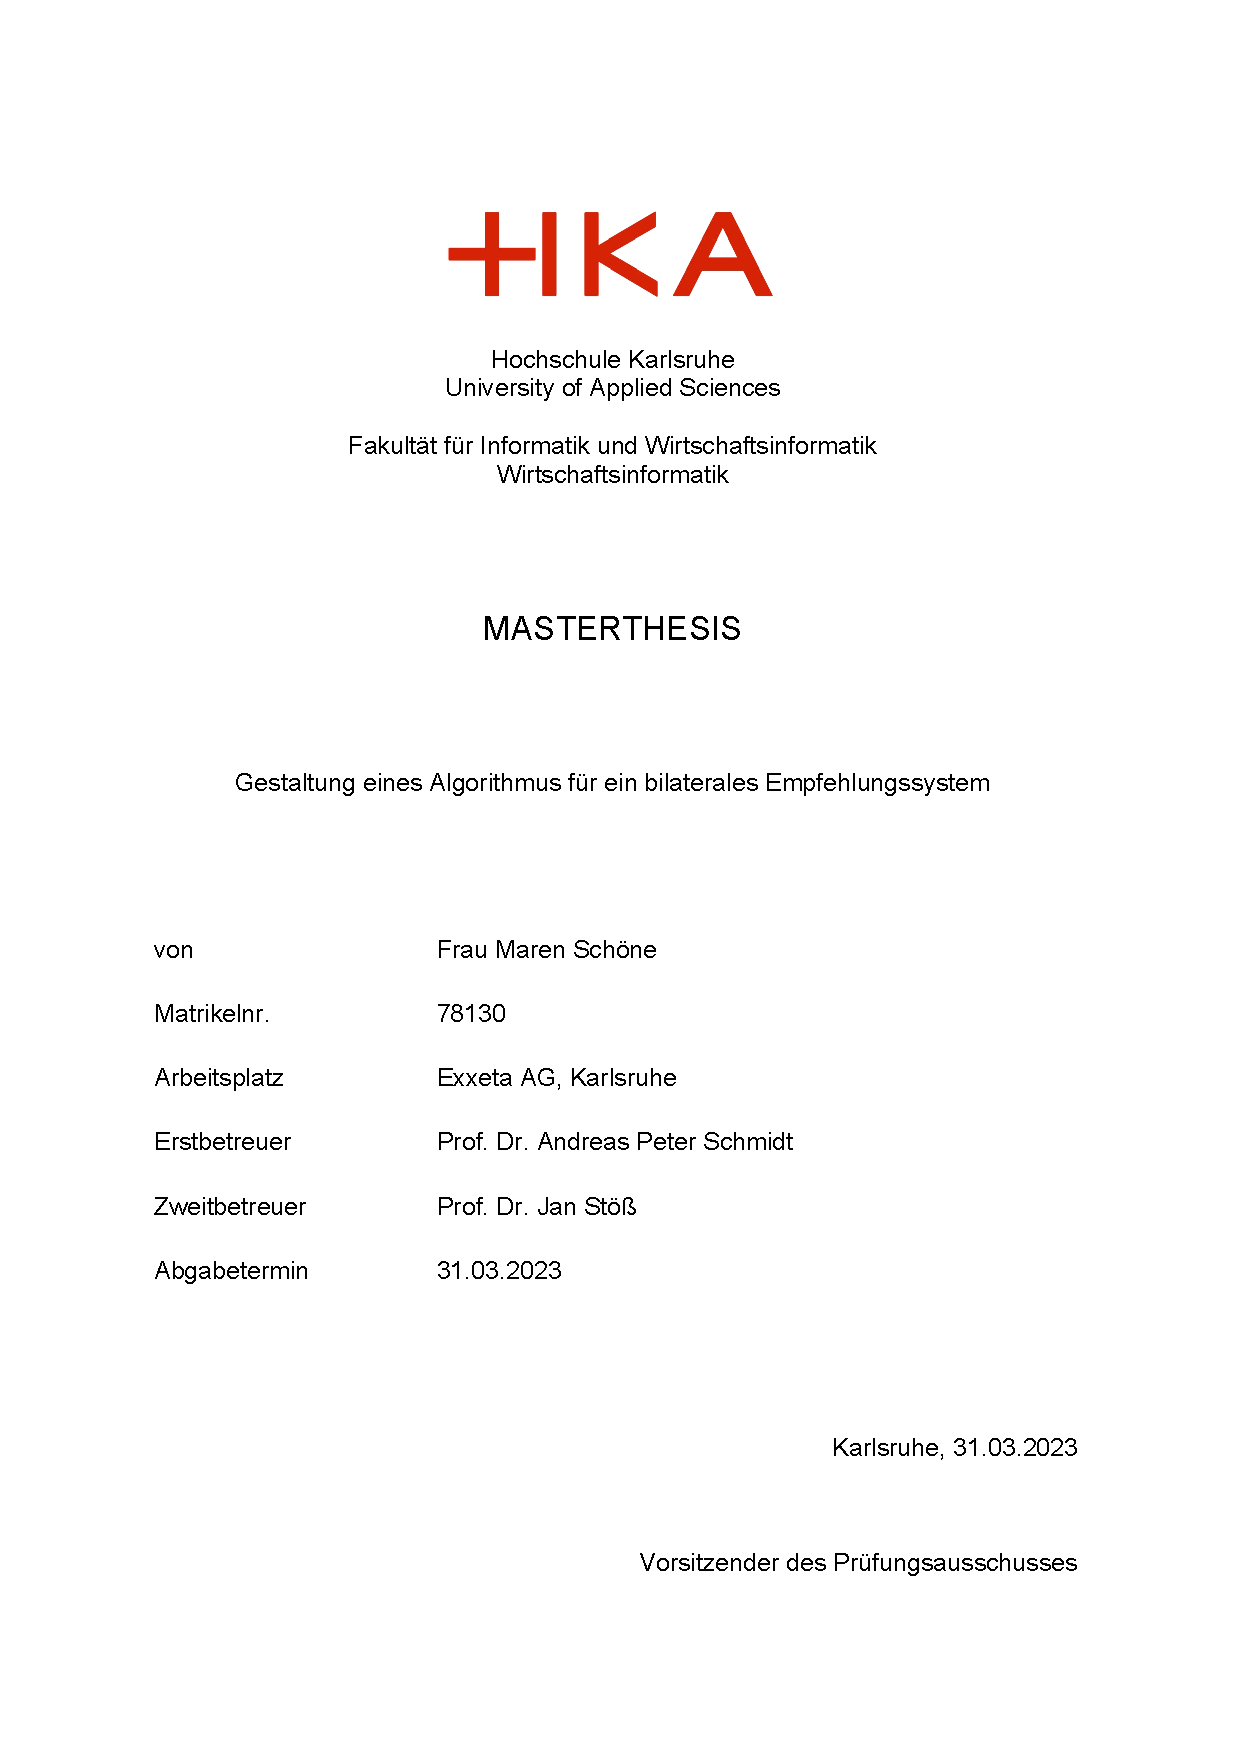
\includepdf[pages=-]{gfx/Deckblatt.pdf}
\end{titlepage}

%%*******************************************************
% Titlepage
%*******************************************************
%%%
%%% title page (german)
%%%
\thispagestyle{empty}
\pdfbookmark[0]{Titelblatt}{title}
\begin{titlepage}

  % If printed on two sides, center the title page
  \condTWOSIDE{\changetext{}{19mm}{}{19mm}{}}

  \vspace{1cm}
  \begin{center}
  	
\includegraphics[width=2.5cm]{gfx/HKA_Logo} \\ 
  \end{center}
  
  \begin{center}
    \huge \textbf{\myUni}\\
    %\huge \textbf{Technik und Wirtschaft}\\
    \vspace{0.4cm}
    \LARGE \myFaculty
  \end{center}

  \vfill
  \vfill

  \begin{center}
    \LARGE \textbf{\myTitle}
  \end{center} 

  \vfill
  \vfill

  \begin{center}
    \Large Abschlussarbeit zur Erlangung des akademischen Grades \textbf{\myDegree}
  \end{center}

  \vfill

  \begin{center}
    \Large vorgelegt von\\
    \vspace{0.3cm}
    \Large \textbf{\myName}\\
    \vspace{0.3cm}
    \normalsize Matrikelnummer: \myId
  \end{center}

  \vfill
  \vfill

  \begin{center}
    \begin{tabular}{lll}
      Referent    & : & \myProf \\
      Korreferent & : & \myOtherProf
    \end{tabular}
  \end{center} 

  % If printed on two sides, center the title page
  \condTWOSIDE{\changetext{}{-19mm}{}{-19mm}{}}

\end{titlepage}

\thispagestyle{empty}

\hfill

\vfill

\noindent\myName: \textit{\myTitle}, \ifdef{\mySubtitle}{\mySubtitle,}{} %\myDegree,
\textcopyright\ \myTime

%\bigskip
%
%\noindent\spacedlowsmallcaps{Supervisors}: \\
%\myProf \\
%\myOtherProf \\
%\mySupervisor
%
%\medskip
%
%\noindent\spacedlowsmallcaps{Location}: \\
%\myLocation
%
%\medskip
%
%\noindent\spacedlowsmallcaps{Time Frame}: \\
%\myTime

%\cleardoublepage\include{frontbackmatter/Dedication}
%\cleardoublepage\include{frontbackmatter/Foreword}
\cleardoublepage%*******************************************************
% Declaration
%*******************************************************
\refstepcounter{dummy}
\pdfbookmark[0]{Declaration}{declaration}
\chapter*{\condENGLISH{Declaration}{Erklärung}}
\thispagestyle{empty}
Ich versichere hiermit, dass ich die vorliegende Arbeit selbständig verfasst und keine anderen als die im Literaturverzeichnis angegebenen Quellen benutzt habe.
\medskip

\noindent
Alle Stellen, die wörtlich oder sinngemäß aus veröffentlichten oder noch nicht veröffentlichten Quellen entnommen sind, sind als solche kenntlich gemacht.
\medskip

\noindent
Die Zeichnungen oder Abbildungen in dieser Arbeit sind von mir selbst erstellt worden oder mit einem entsprechenden Quellennachweis versehen.
\medskip

\noindent
Diese Arbeit ist in gleicher oder ähnlicher Form noch bei keiner anderen Prüfungsbehörde eingereicht worden. 
\bigskip

\noindent\textit{\myLocation, \myTime}

\smallskip

\begin{flushright}
    \begin{tabular}{m{5cm}}
        \\ \hline
        \centering\myName \\
    \end{tabular}
\end{flushright}

%\cleardoublepage%*******************************************************
% Genderhinweis
%*******************************************************
\refstepcounter{dummy}
\pdfbookmark[0]{Declaration}{declaration}
\chapter*{Gleichstellungsklausel}
\thispagestyle{empty}
Für eine bessere Lesbarkeit wird in dieser Arbeit bei Personenbezeichnungen und personenbezogenen Hauptwörtern die männliche Form verwendet. Entsprechende Begriffe gelten gleichermaßen für alle Geschlechter und beinhalten keine Wertung.

%\cleardoublepage%*******************************************************
% Abstract in English
%*******************************************************
\pdfbookmark[1]{Abstract}{Abstract}


\begin{otherlanguage}{american}
	\chapter*{Abstract}
	Short summary of the contents in English. Approximately one page\dots
	\medskip
	
	\noindent
	BTW: A great guide by Kent Beck how to write good abstracts can be found here:
	\begin{center}
		\url{https://plg.uwaterloo.ca/~migod/research/beckOOPSLA.html}
	\end{center}
\end{otherlanguage}
%\cleardoublepage%*******************************************************
% Abstract in German
%*******************************************************
\begin{otherlanguage}{ngerman}
\pdfbookmark[1]{Zusammenfassung}{Zusammenfassung}
\chapter*{Zusammenfassung}
Der Einsatz von Empfehlungssystemen zur Entscheidungsunterstützung hat in den vergangenen Jahren zunehmend an Bedeutung gewonnen.
Während Empfehlungssysteme ursprünglich für die Empfehlung von Gegenständen oder Dokumenten eingesetzt wurden, hat die Empfehlung von Personen durch den Zuwachs an sozialen Netzwerken vermehrt Aufmerksamkeit erlangt.
In Systemen, in denen Personen die Inhalte von Empfehlungen bilden, kann der Erfolg einer Empfehlung von der Erfüllung der Präferenzen beider beteiligter Parteien, das heißt von sowohl Empfehlungsempfänger als auch empfohlener Person, beeinflusst werden.
Solche Systeme werden als wechselseitige oder auch bilaterale Empfehlungssysteme bezeichnet.

In projektgetriebenen Unternehmen können wechselseitige Empfehlungssysteme Entscheidungsträger darin unterstützen, passende Mitarbeiter offenen Projektpositionen zuzuordnen.
% In der Forschung konnte bereits nachgewiesen werden, dass eine beidseitige Berücksichtigung der Bedürfnisse bei der Empfehlungserstellung im Vergleich zu einer unilateralen Berücksichtigung zu einer Verbesserung der Zufriedenheit von Mitarbeitern sowie der erwarteten Arbeitsleistung dieser führen kann.
Nach aktuellem Stand der Forschung blieb bislang unklar, wie die Präferenzen von Entscheidungsträgern und Mitarbeitern in einem bilateralen Empfehlungssystem einfliessen müssten, um die Zufriedenheit der Mitarbeiter und deren erwartete Arbeitsleistung seitens der Entscheidungsträger bei der Zuordnung der Mitarbeiter zu Projektpositionen robust zu verbessern.
Dieser Fragestellung soll im Rahmen der vorliegenden Arbeit nachgegangen werden.

Hierfür wurde ein multi-kriterieller Ansatz für die Berücksichtigung der Präferenzen von Entscheidungsträgern und Mitarbeitern bei der Zuordnung zu Projekten konzipiert.
Innerhalb des Systems wurde ein bilateraler Algorithmus implementiert, der Empfehlungen anhand der gewichteten Summe der Präferenzerfüllung eines Mitarbeiters und der Präferenzerfüllung eines Entscheidungsträgers ermittelt.
Dessen Tauglichkeit wurde im Rahmen eines Experiments mit einem unilateralen Algorithmus verglichen, welcher lediglich die Bedürfnisse der Entscheidunsträger betrachtet.

Insgesamt zeigten die Ergebnisse des Experiments, dass eine Berücksichtigung der beidseitigen Präferenzen bei der Zuordnung von Mitarbeitern zu Projektpositionen grundsätzlich vorteilhaft ist.
Jedoch konnten einzelne Ausreißer in den Ergebnissen festgestellt werden, bei denen unter diesen Bedingungen eine geringere Zufriedenheit bzw. Arbeitsleistung verzeichnet wurde.
Eine Robustheit des entwickelten Ansatzes kann daher nicht uneingeschränkt bestätigt werden.

Als Ursache für diese Beobachtung wird vermutet, dass sowohl die Zufriedenheit von Mitarbeitern als auch deren erwartete Arbeitsleistung seitens der Entscheidungsträger durch weitere Einflussfaktoren bestimmt werden.
Um den eindeutigen Einfluss der bilateralen Präferenzerfüllung auf Zufriedenheit und Arbeitsleistung zu ermitteln, wird empfohlen, diese Faktoren durch das Durchführen von Experteninterviews unter den Managern und Mitarbeitern zu identifizieren.
Die identifizierten Faktoren sollten in weiterführenden Forschungen als zusätzliche Kriterien des multi-kriteriellen Empfehlungssystems berücksichtigt werden.

Bezüglich der Gewichtung der Präferenzen wurde im Rahmen des Experiments deutlich, dass es eine geringfügigere Rolle spielt, wie die Präferenzen von Entscheidungsträgern bzw. Mitarbeitern gewichtet werden.
Um den Effekt der Gewichtung auf Zufriedenheit und Arbeitsleistung genauer zu untersuchen, wird für weiterführende Forschungen empfohlen, die Fälle genauer zu betrachten, in denen die Bedürfnisse der Entscheidungsträger und die Bedürfnisse der Mitarbeiter miteinander konkurrieren.
Darüber hinaus sollte in zukünftigen Studien die optimalen Gewichtung der Präferenzen anhand einer größeren Datenbasis ermittelt werden, um den Algorithmus gegenüber Ausreißer robuster zu gestalten.

\end{otherlanguage}

%\cleardoublepage%*******************************************************
% Publications
%*******************************************************
\pdfbookmark[1]{Publications}{publications}
\chapter*{Publications}\graffito{This is just an early --~and currently ugly~-- test!}
This might come in handy for PhD theses: some ideas and figures have appeared previously in the following publications:

%\noindent Put your publications from the thesis here. The packages \texttt{multibib} or \texttt{bibtopic} etc. can be used to handle multiple different bibliographies in your document.

\begin{refsection}[ownpubs]
    \small
    \nocite{*} % is local to to the enclosing refsection
    \printbibliography[heading=none]
\end{refsection}

\emph{Attention}: This requires a separate run of \texttt{bibtex} for your \texttt{refsection}, \eg, \texttt{ClassicThesis1-blx} for this file. You might also use \texttt{biber} as the backend for \texttt{biblatex}. See also \url{http://tex.stackexchange.com/questions/128196/problem-with-refsection}.

%\cleardoublepage%*******************************************************
% Acknowledgments
%*******************************************************
\pdfbookmark[1]{Acknowledgments}{acknowledgments}

\begin{flushright}{\slshape
    We have seen that computer programming is an art, \\
    because it applies accumulated knowledge to the world, \\
    because it requires skill and ingenuity, and especially \\
    because it produces objects of beauty.} \\ \medskip
    --- \defcitealias{knuth:1974}{Donald E. Knuth}\citetalias{knuth:1974} \citep{knuth:1974}
\end{flushright}



\bigskip

\begingroup
\let\clearpage\relax
\let\cleardoublepage\relax
\let\cleardoublepage\relax
\chapter*{Acknowledgments}
Put your acknowledgments here.

Many thanks to everybody who already sent me a postcard!

Regarding the typography and other help, many thanks go to Marco 
Kuhlmann, Philipp Lehman, Lothar Schlesier, Jim Young, Lorenzo 
Pantieri and Enrico Gregorio\footnote{Members of GuIT (Gruppo 
Italiano Utilizzatori di \TeX\ e \LaTeX )}, J\"org Sommer, 
Joachim K\"ostler, Daniel Gottschlag, Denis Aydin, Paride 
Legovini, Steffen Prochnow, Nicolas Repp, Hinrich Harms, 
Roland Winkler, Jörg Weber, Henri Menke, Claus Lahiri, 
Clemens Niederberger, Stefano Bragaglia, Jörn Hees, 
Scott Lowe, Dave Howcroft, 
and the whole \LaTeX-community for support, ideas and 
some great software.

\bigskip

\noindent\emph{Regarding \mLyX}: The \mLyX\ port was intially done by
\emph{Nicholas Mariette} in March 2009 and continued by
\emph{Ivo Pletikosi\'c} in 2011. Thank you very much for your
work and for the contributions to the original style.


\endgroup




\cleardoublepage%*******************************************************
% Table of Contents
%*******************************************************
\pagestyle{scrheadings}
\refstepcounter{dummy}
\pdfbookmark[1]{\contentsname}{tableofcontents}
\setcounter{tocdepth}{4} % <-- 2 includes up to subsections in the ToC
\setcounter{secnumdepth}{4} % <-- 3 numbers up to subsubsections
\manualmark
\markboth{\spacedlowsmallcaps{\contentsname}}{\spacedlowsmallcaps{\contentsname}}
\tableofcontents

\cleardoublepage
\cleardoublepage%*******************************************************
% List of Figures
%*******************************************************    
\automark[section]{chapter}
\renewcommand{\chaptermark}[1]{\markboth{\spacedlowsmallcaps{#1}}{\spacedlowsmallcaps{#1}}}
\renewcommand{\sectionmark}[1]{\markright{\thesection\enspace\spacedlowsmallcaps{#1}}}
\refstepcounter{dummy}
\pdfbookmark[1]{\listfigurename}{lof}
\listoffigures

\cleardoublepage

\cleardoublepage%*******************************************************
% List of Tables
%*******************************************************
\automark[section]{chapter}
\renewcommand{\chaptermark}[1]{\markboth{\spacedlowsmallcaps{#1}}{\spacedlowsmallcaps{#1}}}
\renewcommand{\sectionmark}[1]{\markright{\thesection\enspace\spacedlowsmallcaps{#1}}}
\refstepcounter{dummy}
\pdfbookmark[1]{\listtablename}{lot}
\listoftables

\cleardoublepage
\cleardoublepage%*******************************************************
% List of Listings
%*******************************************************      
\automark[section]{chapter}
\renewcommand{\chaptermark}[1]{\markboth{\spacedlowsmallcaps{#1}}{\spacedlowsmallcaps{#1}}}
\renewcommand{\sectionmark}[1]{\markright{\thesection\enspace\spacedlowsmallcaps{#1}}}
\refstepcounter{dummy}
\pdfbookmark[1]{\lstlistlistingname}{lol}
\lstlistoflistings

\cleardoublepage
\cleardoublepage%*******************************************************
% Acronyms
%*******************************************************
\automark[section]{chapter}
\renewcommand{\chaptermark}[1]{\markboth{\spacedlowsmallcaps{#1}}{\spacedlowsmallcaps{#1}}}
\renewcommand{\sectionmark}[1]{\markright{\thesection\enspace\spacedlowsmallcaps{#1}}}
\refstepcounter{dummy}
\pdfbookmark[1]{Abk\"{u}rzungsverzeichnis}{abk\"{u}rzungsverzeichnis}
\markboth{\spacedlowsmallcaps{Abk\"{u}rzungsverzeichnis}}{\spacedlowsmallcaps{Abk\"{u}rzungsverzeichnis}}
\chapter*{Abk\"{u}rzungsverzeichnis}

% Insert your acronyms here
\begin{acronym}[AWGN]%[UML]
  \acro{ESCO}[ESCO]{European Skills/Competences, Qualifications and Occupations}
  %\acro{JES}[JES]{Java Enterprise Solutions}
  \acro{JSON}[JSON]{JavaScript Object Notation}
  \acroplural{JSON}[JSONs]{JSONs}
  \acro{KNN}[KNN]{$k$-nächste Nachbarn}
  \acro{NNA}[NNA]{Nächste Nachbar Analyse (Nearest Neighbor Analysis)}
  \acro{ONet}[O*Net]{Occupational Information Network}
  \acro{PEFit}[P-E Fit]{Person-Environment Fit}
  \acroplural{PEFit}[P-E Fits]{Person-Environment Fits}
  \acro{PJFit}[P-J Fit]{Person-Job Fit}
  \acroplural{PJFit}[P-J Fits]{Person-Job Fits}
  \acro{PCA}[PCA]{Principal Component Analysis}
  \acro{REST}[REST]{Representational State Transfer}
\end{acronym}

\cleardoublepage

%*************************************************************************
% Mainmatter
%*************************************************************************
\cleardoublepage
\pagestyle{scrheadings}
\pagenumbering{arabic}
% Alwas use \cleardoublepage before \part{...}.
\cleardoublepage
\part{Thesis}\label{pt:thesis}
\shorthandoff{"}
\chapter{Einführung}
\label{ch:intro}

\section{Motivation}
\label{sec:intro:motivation}
In Unternehmen aller Branchen ist eine Abkehr von großgewachsenen, zentralen und hierarchischen Organisationsstrukturen zu beobachten. Stattdessen setzen Betriebe zunehmend auf kleine, dezentrale und flexible Teams, welche in Projektarbeiten neue Produkte entwickeln und Dienstleistungen erbringen \cite[S. 3]{elanceEconomy:1999}. Besonders stark nimmt dieser Trend seit Mitte der 1990er Jahre zu \cite[S. 8]{whittington:1999}. Ein Hauptgrund für den Wandel ist die fortschreitende Digitalisierung. Diese ermöglicht kurze Kommunikations- und Entscheidungswege und macht damit zentrale und hierarchische Unternehmensstrukturen zunehmend überflüssig \cite[S. 5]{elanceEconomy:1999}.

Aufgrund dieser Entwicklungen wird die Zusammenstellung von Mitarbeitern für neue Projekte voraussichtlich ein immer häufiger stattfindender Prozess in der Wirtschaft sein. Unterstützung können dabei Empfehlungssysteme im Bereich der Personalauswahl bieten. In der Literatur existieren bereits einige Ansätze zur Implementierung solcher Anwendungen. \textcite[S. 1ff.]{malinowski:2006} zu Folge bieten bestehende Empfehlungssysteme jedoch häufig unzureichende Lösungen, da sich diese zumeist einseitig entweder an Personalverantwortliche oder an Stellensuchende richten. Die Wissenschaftler empfehlen stattdessen die Implementierung bilateraler Empfehlungssysteme. Dieses Konzept basiert auf der Theorie des \acp{PEFit} aus der Berufs- und Organisationspsychologie \cite[S. 2]{guan:2021}\cite[S. 3.f]{malinowski:2006}. Es besagt, dass Mitarbeiter und Personalverantwortliche jeweils eine Angebots- und eine Nachfrageperspektive besitzen. Gleichen sich Angebot und Nachfrage beider Parteien aus, führt dies aus Sicht des Unternehmens zu einer hohen Arbeitsleistung und zugleich aus Perspektive des Mitarbeiters zu einer ausgeprägten Zufriedenheit \cite[S. 6]{su:2015}.

Bisher belegte jedoch noch keine Publikation, dass die Theorie des \acp{PEFit} und die damit verbundenen Ergebnisse auf Seiten von Mitarbeitern und Personalverantwortlichen auch durch Empfehlungssysteme erzielt werden können. Somit ist nicht nachgewiesen, dass der höhere Aufwand zur Implementierung bilateraler Anwendungen gegenüber unilateralen Systemen zur Besetzung offener Projektpositionen gerechtfertigt ist. Diese Forschungslücke soll im Rahmen dieser Master-Thesis geschlossen werden.

\newpage
\section{Zielsetzung}
\label{sec:intro:zielsetzung}
Das Ziel der vorliegenden Master-Thesis besteht darin, die folgende Forschungsfrage zu beantworten:

\forschungsfrage

Um diese Frage zu beantworten, wird ein Experiment mit einer anschließenden Fallstudie durchgeführt. Dabei werden Mitarbeiter eines Beratungsunternehmens im IT-Bereich sowohl von einem uni- als auch von einem bilateralen Empfehlungsverfahren für verschiedene Projektpositionen vorgeschlagen. Anschließend wird evaluiert, ob die verantwortlichen Projektmanager von den empfohlenen Angestellten der bilateralen Anwendung eine höhere Arbeitsleistung erwarten, als von den Vorschlägen des unilateralen Systems. Außerdem wird überprüft, ob die Mitarbeiter zufriedener mit ihrer Positionierung in den Vorschlägen der bilateralen Anwendung sind.

\section{Gang der Arbeit}
\label{sec:intro:gangDerArbeit}
Um die Forschungsfrage der vorliegenden Master-Thesis zu beantworten, werden in den Kapiteln \ref{ch:personEnvironmentFit} und \ref{ch:empfehlungssysteme} zunächst die theoretischen Grundlagen bilateraler Empfehlungssysteme erläutert. Hierzu wird in Kapitel \ref{ch:personEnvironmentFit} das psychologische Konzept des \acp{PEFit} erörtert. Das folgende Kapitel \ref{ch:empfehlungssysteme} enthält einen Überblick über Implementierungsansätzen von Empfehlungssystemen. Dabei werden neben modell- und speicherbasierten Methoden auch hybride Verfahren erläutert. Darüber hinaus werden häufig auftretende Probleme bei der Entwicklung von Empfehlungssystemen geschildert und entsprechende Lösungsmöglichkeiten aufgezeigt. Im folgenden Kapitel \ref{ch:verwandteArbeiten} wird der aktuelle Stand der Forschung behandelt. In diesem Kontext werden verwandte Arbeiten diskutiert und hinsichtlich der Forschungsfrage analysiert. Anschließend wird in Kapitel \ref{ch:methodik} die Methodik der Master-Thesis erläutert. In diesem Zusammenhang werden die implementierte Systemarchitektur und die Gestaltung der Fallstudie dargelegt. Die bei Durchführung der Studie gewonnenen Ergebnisse werden in Kapitel \ref{ch:ergebnisse} vorgestellt. Eine Diskussion der Erkenntnisse findet sich im darauffolgenden Kapitel \ref{ch:diskussion}. Dieses endet mit der Beantwortung der Forschungsfrage und daraus abgeleiteten Empfehlungen für zukünftige Arbeiten. Ein abschließendes Fazit folgt in Kapitel \ref{ch:fazit}.
\shorthandon{"}
\shorthandoff{"}
\chapter{Person-Environment Fit}
\label{ch:personEnvironmentFit}

\section{Einführung}
\label{ch:personEnvironmentFit:einfuehrung}
Der \acf{PEFit} ist ein Konzept, welches häufig im Kontext der Berufs- und Organisationspsychologie Anwendung findet \cite[S. 2]{guan:2021}. In manchen Publikationen existiert die Theorie auch unter ähnlichen Bezeichnungen mit derselben Bedeutung wie Person-Environment Korrespondenz \cite[S. 1]{eggerth:2008} oder -Kongruenz \cite[S. 1]{muchinsky:1987}. Es enthält drei zentrale Größen: Person, Umgebung (Environment) und Ergebnis \cite[S. 2]{livingstone:1997}.

\textcite[S. 5]{edwards:2007} stellten fest, dass die Literatur unter der Person ein menschliches Individuum versteht. Umgebung und Ergebnis werden ihren Beobachtungen zu Folge dagegen als breite Terminologien interpretiert und je nach Forschungsdomäne genauer spezifiziert \cite[S. 1ff.]{edwards:2007}. Beispiele für Ergebnisse sind Zufriedenheit \cite[S. 1]{lashani:2021}, Wechselbereitschaft \cite[S. 1]{amarneh:2021}, Kreativität \cite[S. 1]{duan:2019}, Leistung \cite[S. 6ff.]{elfenbein:2007} und  Berufswahl \cite[S. 1]{cable:1996}. Als Umgebung untersuchten verschiedene Publikationen unter anderem Unternehmen \cite[S. 1]{kristof:1996}, Gruppen \cite[S. 1]{werbel:2001} und Arbeitsplätze \cite[S. 1]{lu:2014}.

Die Wissenschaft geht davon aus, dass ein Ergebnis stets vom Zusammenspiel von Person und Umgebung abhängig ist und nicht durch eine der beiden Größen alleine bestimmt wird \cite[S. 1f.]{muchinsky:1987}. Wie in Abbildung \ref{fig:personEnvironmentFit:einfuehrung:abb1} verdeutlicht, ist der Fit somit selbst kein Ergebnis, sondern eine unabhängige Variable, welche zur Vorhersage eines untersuchten Resultates herangezogen wird \cite[S. 11]{caplan:1993}\cite[S.5]{edwards:1991}\cite[S. 1]{edwards:2002}.

\begin{figure}[h]
	\centering
	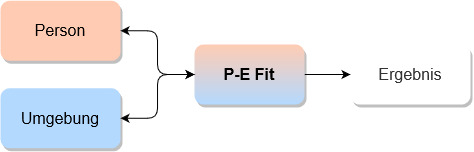
\includegraphics[width=1\textwidth]{gfx/P-E Fit.jpg}
	\caption{Zusammenwirken von Person, Umgebung, \acs{PEFit} und Ergebnis}
	\label{fig:personEnvironmentFit:einfuehrung:abb1}
\end{figure}

Der in Abbildung \ref{fig:personEnvironmentFit:einfuehrung:abb1} dargestellte \ac{PEFit} gibt an, zu welchem Grad sich die untersuchten Werte von Person und Umgebung auf einem Niveau befinden \cite[S. 53]{edwards:2008}. Dabei wird der Fit häufig nicht als Zustand, sondern als wechselseitiger Prozess betrachtet, in dem Person und Umgebung miteinander interagieren und sich dabei gegenseitig verändern \cite[S. 10ff.]{su:2015}. Diese Modifikationen können die Kongruenz sowohl verbessern als auch verschlechtern \cite[S. 4]{caplan:1987}. Aus diesem Grund können Unternehmen auch Maßnahmen ergreifen, welche den \ac{PEFit} gezielt optimieren \cite[S. 16]{cable:2001}.

\textcite[S. 6ff.]{edwards:2007} unterschieden drei Ebenen, auf welchen ein Fit bestimmbar ist. Die oberste bezeichneten sie als globale Ebene. Hier werden Person und Umgebung als Ganzes, ohne weitere Untergliederungen miteinander vergleichen. Von der Domänen-Ebene sprachen \textcite[S. 7f.]{edwards:2007}, wenn eine Einteilung in mehrere sehr breite Bereiche vorgenommen wird, welche stellvertretend für Person und Umgebung miteinander vergleichen werden. Domänen können den Autoren zu Folge beispielsweise Werte, Bildung oder Berufserfahrung sein. Findet die Untersuchung ausschließlich innerhalb einer Domäne statt, bezeichneten \textcite[S. 7f.]{edwards:2007} dies als Facetten-Ebene. Als Beispiel nannten sie die Bestimmung eines \acp{PEFit} hinsichtlich demographischer Ähnlichkeit anhand von Dimensionen wie Alter und Bildung.

Wie die Kongruenz von Person und Umgebung bestimmt wird, ist von der konkreten Art des Fits abhängig. \textcite[S. 1]{muchinsky:1987} unterschieden zwischen ergänzendem und komplementärem Fit.

\section{Ergänzender und komplementärer Fit}
\label{ch:personEnvironmentFit:supplementaryUndComplementary}
Ein ergänzender Fit entsteht, wenn Person und Umgebung gleiche Werte und Interessen aufweisen \cite[S. 2ff.]{muchinsky:1987}. Diese Art der Kongruenz ist laut \textcite[S. 5ff.]{schneider:1987} ein entscheidender Faktor, von welchen Unternehmen sich potentielle Arbeitnehmer angezogen fühlen und welche Bewerber von Betrieben eingestellt werden. \textcite[S. 4, Z. 47f.]{popovich:1982} zu Folge kann der Beitritt einer Person zu einem Unternehmen sogar als ein "sehr konkreter, öffentlicher Ausdruck der Werte"\footnote{"a very concrete, public expression of values" - \textcite[S. 4, Z. 47f.]{popovich:1982}} eines Individuums interpretiert werden.

Verschiedene Autoren diskutierten die Ergebnisse des ergänzenden Fits in der Literatur kontrovers. \textcite[S. 6]{schneider:1987} stellte fest, dass Angestellte mit einer geringen Übereinstimmung ihrer Werte eher dazu tendieren, das Unternehmen zu verlassen. So entsteht dem Autor zu Folge im Betrieb langfristig eine hohe Homogenität innerhalb der Belegschaft. Diese äußert sich einerseits in positiven Ergebnissen wie einer ausgeprägten Arbeitszufriedenheit und einer starken Identifikation mit dem Unternehmen \cite[S. 26]{kristof:1996}. Die mangelnde Diversität führt aber anderseits auch zu negativen Folgen, wie einer geringeren Fähigkeit zu Veränderungen \cite[S. 10]{schneider:1987} und verminderter Kreativität \cite[S. 7]{chatman:1998} und Innovation im Unternehmen \cite[S. 11]{chatman:1989}.

Wenn sich Person und Umgebung nicht ähneln, sondern gegenseitig vervollständigen, sprachen \textcite[S. 4]{muchinsky:1987} vom komplementären Fit. Dabei gleichen Person und Umgebung den Autoren zu Folge Schwächen des anderen durch eigene Stärken aus.

Die komplementäre Kongruenz wird, wie in Abbildung \ref{fig:personEnvironmentFit:supplementaryUndComplementary:abb1} dargestellt, in zwei weitere Fits untergliedert. Bei dieser Betrachtungsweise haben Person und Umgebung je eine Angebots- und eine Nachfrageperspektive. Die Nachfrage der einen Partei wird dabei durch das Angebot der anderen erfüllt. \cite[S. 2ff.]{caplan:1987}\cite[S. 2ff.]{edwards:1991}\cite[S. 2]{copingAndAdaption:1974}\cite[S. 3f.]{kristof:1996}

\begin{figure}[h]
	\centering
	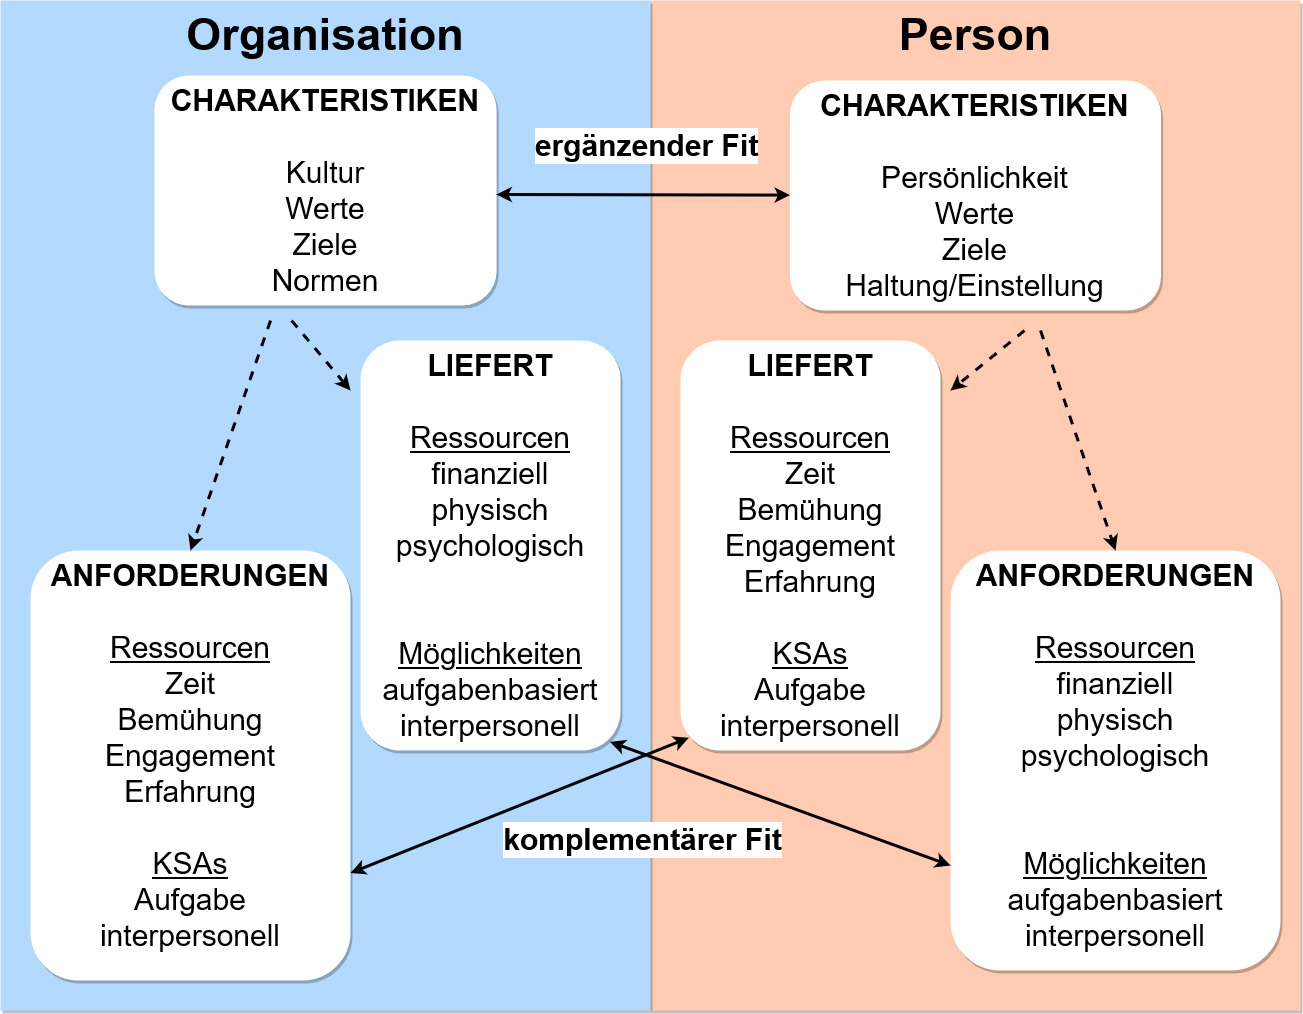
\includegraphics[width=1\textwidth]{gfx/supplementaryComplementaryFit.jpg}
	\caption[Ergänzender und komplementärer \acs{PEFit}]{Ergänzender und komplementärer \acs{PEFit}\\
	(Eigene Darstellung in Anlehnung an \cite[S. 4]{kristof:1996})}
	\label{fig:personEnvironmentFit:supplementaryUndComplementary:abb1}
\end{figure}

Unter der in Abbildung \ref{fig:personEnvironmentFit:supplementaryUndComplementary:abb1} dargestellten Nachfrage der Umgebung werden Anforderungen an die Person zusammengefasst. Hierzu zählen beispielsweise Rollen- und Leistungserwartungen. Das entsprechende Angebot der Person umfasst Fähigkeiten, Fertigkeiten, Wissen, Bildung und Arbeitserfahrung. Gleichen sich Nachfrage der Umgebung und Angebot der Person gegenseitig aus, entsteht der Anforderungen-Fähigkeiten Fit. Dieser resultiert in einer hohen Leistung und Effizienz von Individuum und Umgebung. \cite[S. 3f.]{edwards:1991}\cite[S. 5f.]{edwards:1996}\cite[S. 4]{edwards:2007}\cite[S. 7]{su:2015}

Die Nachfrage der Person in Abbildung \ref{fig:personEnvironmentFit:supplementaryUndComplementary:abb1} entspricht ihren psychologischen Bedürfnissen. Dazu zählen persönliche Präferenzen, Interessen, Motive und Ziele. Die entsprechenden Angebote der Umgebung umfassen Ressourcen und Belohnungen wie Gehalt und Mitbestimmungsrechte, welche die Bedürfnisse des Individuums befriedigen sollen. Sind Nachfrage der Person und Angebot der Umgebung gleich stark ausgeprägt, wird dies in der Literatur als Bedürfnisse-Angebote Fit bezeichnet. Dieser resultiert in einem hohen Wohlbefinden des Mitarbeiters, welches sich beispielsweise in Zufriedenheit und verminderter Wechselbereitschaft äußert. \cite[S. 2]{edwards:2004}\cite[S. 2f.]{edwards:1996}\cite[S. 4]{edwards:2008}\cite[S. 4f.]{edwards:2007}\cite[S. 7]{su:2015}

Laut \textcite[S. 12ff.]{workAdjustment:1964} führen unausgeglichene Nachfragen langfristig zu einem Wechsel des Arbeitsplatzes. Die Autoren betrachteten die aus unzureichend erfüllten Anforderungen des Unternehmens entstehende mangelnde Arbeitsleistung als Ursache für Kündigung oder Versetzung des Mitarbeiters seitens des Arbeitgebers. Die Unzufriedenheit, welche aus unzureichend erfüllten Bedürfnissen des Angestellten resultiert, bezeichneten sie als einen Wechselgrund seitens des Mitarbeiters.

\textcite[S. 1, Z. 2]{edwards:2004} charakterisierten ergänzende und komplementäre Kongruenz als "parallele, aber unterschiedliche Strömungen"\footnote{"parallel but separate streams" - \textcite[S. 1, Z. 2]{edwards:2004}} innerhalb der \ac{PEFit}-Forschung. Doch sie stellten fest, dass beide Fits nicht vollkommen unabhängig voneinander sind. Die Ursache sahen sie in den inneren Werten von Person und Umgebung. Diese sind den Autoren zu Folge einerseits ausschlaggebend für den ergänzenden Fit, beeinflussen aber auch stark die Bedürfnisse der Person und die Angebote der Umgebung \cite[S. 3]{edwards:2004}. Beispielsweise könnte sich ein Individuum mit ausgeprägten familiären Werten aufgrund des ergänzenden Fits stark zu Betrieben mit einer gemeinschaftlichen Unternehmenskultur angezogen fühlen. Gleichzeitig prägt die Person aufgrund ihrer inneren Werte im komplementären Fit das Bedürfnis nach familiären Reizen wie gemeinsamen Veranstaltungen aus. Da das Unternehmen dieselben Eigenschaften besitzt, wird es eher dazu tendieren, seinen Mitarbeitern die Teilnahme an solchen Ereignissen anzubieten.

Dass der Abgleich der Charakteristiken von Person und Umgebung sehr bedeutsam für Zufriedenheit und Produktivität ist, erkannten Psychologen bereits vor über einhundert Jahren \cite[S. 3ff.]{parsons:1909}. Die Wurzeln des \acp{PEFit} reichen zurück bis ins Jahr 1909 \cite[S. 1]{su:2015}.

\section{Historische Entwicklung}
\label{ch:personEnvironmentFit:historisches}
Zu Beginn des 20. Jahrhunderts beschäftigten sich Wissenschaftler und Psychologen in zahlreichen Ländern der westlichen Welt intensiv mit dem Thema der Personalauswahl \cite[S. 1f.]{salgado:2001}. Ein Hauptanliegen der Forscher war es, individuelle Unterschiede zwischen den Menschen anzuerkennen \cite[S. 1ff.]{stern:1900}. Deren Ansichten zu Folge würde die gesamte Gesellschaft effizienter arbeiten, wenn Männer eine zu ihren wissenschaftlich ermittelten Fähigkeiten passende Tätigkeit aufnehmen würden \cite[S. 1f.]{kevles:1968}. Im Zuge dieser Entwicklungen konzipierte der Bostoner Professor Frank Parsons eine Vorgehensweise zur Berufsfindung, welche im Jahr 1909 vorgestellt wurde \cite[S. 3]{porfeli:2009}\cite[S. 1]{su:2015}. \textcite[S. 5ff.]{parsons:1909} erkannte schon zum damaligen Zeitpunkt, dass die Beziehung zwischen eigenen Fähigkeiten und Anforderungen des Berufsumfeldes eine wichtige Ursache für Effizienz, Produktqualität und Bezahlung waren. Aus diesem Grund empfahl er jungen Männern vor der Berufswahl zunächst ihre eigenen Fähigkeiten, die Anforderungen verschiedener Arbeitsplätze und die Beziehung zwischen beiden Seiten zu verstehen. Erst wenn sie diese Punkte unter Beaufsichtigung eines Berufsberaters und durch Verwendung verschiedener wissenschaftlicher Tests erfüllen, können sie sich dem Autor zu Folge für einen passenden Beruf entscheiden \cite[S. 5ff.]{parsons:1909}. Heute gilt Parsons aufgrund dieser Gedanken als "Gründungsvater der Berufsberatung"\footnote{"founding father of vocational guidance" - \textcite[S. 3, Z. 29]{porfeli:2009}} \cite[S. 3, Z. 29]{porfeli:2009} und als wichtiger Vorläufer des \acp{PEFit} \cite[S. 2]{edwards:2008}\cite[S. 1]{su:2015}.

Zum damaligen Zeitpunkt begegnete die Bevölkerung den neuartigen psychologischen Tests zunächst mit Skepsis \cite[S. 2]{kevles:1968}. Das änderte sich insbesondere im Jahr 1917 mit dem Eintritt der Vereinigten Staaten in den Ersten Weltkrieg. Das U.S. Militär stand vor der Herausforderung, innerhalb kürzester Zeit Millionen Männer in die verschiedenen spezialisierten Rollen des technisierten Krieges einzuordnen. Zu diesem Anlass setzten Wissenschaftler erstmals im großen Stil psychologische Tests zur Zuweisung von Personen zu passenden Militärpositionen ein \cite[S. 2ff.]{kevles:1968}. 

Nach dem Ersten Weltkrieg entstanden insbesondere in den 1930er-Jahren durch die Arbeiten von Kurt Lewin und Henry Murray weitere bedeutende Entwicklungen für die Entstehung des \acp{PEFit} \cite[S. 1]{edwards:1990}\cite[S. 5]{caplan:1993}. \textcite[S. 11f.]{lewin:1936} stellte fest, dass das Verhalten eines Menschen nicht nur durch das Individuum selbst, sondern durch das Zusammenspiel von Person und Umgebung zu erklären ist. Ergänzend zu diesen Erkenntnissen erarbeitete Murray sein Need-Press-Modell \cite[S. 2]{edwards:2008}. Der Wissenschaftler ging davon aus, dass jeder Mensch im Laufe seines Lebens verschiedene Bedürfnisse (Needs) unterschiedlich stark ausprägt. Diese treffen je nach Umgebung auf diverse Reize. Murray stellte fest, dass manche Reize mit bestimmten Bedürfnissen kompatibel sind. Trifft ein passendes Bedürfnis-Reiz-Paar aufeinander, entsteht Druck (Press). Personen interpretieren diesen subjektiv als schädliche oder nützliche Situation und zeigen dem Autor zu Folge eine entsprechende Reaktion \cite[S. 38ff.]{murray:1938}. Dieses Zusammenspiel von Bedürfnissen einer Person und Reizen der Umgebung entspricht der späteren Vorstellung des Bedürfnisse-Angebote Fits \cite[S. 8]{edwards:2008}. 

Die Erkenntnisse von Lewin und Murray gelten als wichtiger Grundstein für die Arbeiten verschiedener Forschungsgruppen rund um John R. P. French, Jr. \cite[S. 5]{caplan:1993}. Der Psychologe stellte im Jahr 1963 an der Universität in Michigan ein groß angelegtes Forschungsprogramm vor, in welchem Experten unterschiedlicher Fachrichtungen eng zusammenarbeiteten. Diese machten es sich zum Ziel, die Auswirkungen des sozialen Umfeldes in Industrieunternehmen auf die Gesundheit der Mitarbeiter zu untersuchen \cite[S. 1ff.]{french:1963}. Aus dieser Kollaboration entstanden wesentliche Beiträge zur Entstehung des \acp{PEFit} \cite[S. 4ff.]{caplan:1993}. Hierbei unterschieden die Forscher zunächst zwischen objektivem und subjektivem Fit \cite[S. 4f.]{caplan:1993}\cite[S. 1ff.]{copingAndAdaption:1974}\cite[S. 1ff.]{french:1966}.

\section{Objektiver und subjektiver P-E Fit}
\label{ch:personEnvironmentFit:subjektivObjektiv}
Wie in Abbildung \ref{fig:personEnvironmentFit:subjektivObjektiv:abb1} dargestellt, gingen \textcite[S. 1ff.]{copingAndAdaption:1974} davon aus, dass von Person und Umgebung je eine objektiv messbare und eine vom Individuum subjektiv wahrgenommene Version existieren.

\begin{figure}[h]
	\centering
	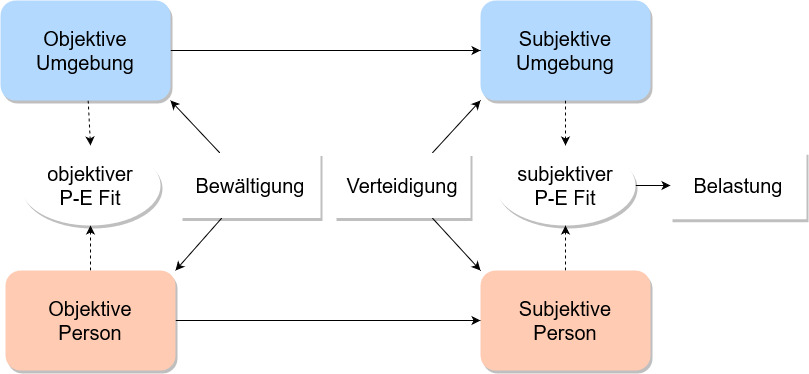
\includegraphics[width=1\textwidth]{gfx/subjektivObjektivPEFit.jpg}
	\caption[Objektiver und subjektiver \acs{PEFit}]{Objektiver und subjektiver \acs{PEFit}\\
	(Eigene Darstellung in Anlehnung an \cite[S. 22]{edwards:2008})}
	\label{fig:personEnvironmentFit:subjektivObjektiv:abb1}
\end{figure}
%TODO: Hier vlt eher Originalquelle

Die Forscher bemerkten, dass insbesondere der in Abbildung \ref{fig:personEnvironmentFit:subjektivObjektiv:abb1} dargestellte subjektive \ac{PEFit} bedeutsam für die Entstehung psychischer Belastungen ist. Die objektive Kongruenz spielt den Autoren zu Folge dagegen eine untergeordnete Rolle \cite[S. 4]{copingAndAdaption:1974}. Auch Publikationen anderer Forscher bestätigten diese Einschätzung \cite[S. 3]{carless:2005}. Dementsprechend wird die subjektive Wahrnehmung des \acp{PEFit} in der Literatur stärker fokussiert \cite[S. 8]{caplan:1987}\cite[S. 9]{caplan:1993}\cite[S. 16]{choi:2004}.

In einer auf den Erkenntnissen von French Jr., Rodergs und Cobb aufbauenden Arbeit kam \textcite[S. 5ff.]{harrison:1978} sogar zu der Einschätzung, dass innerhalb des subjektiven \acp{PEFit} alleine die Bedürfnisse-Angebote Kongruenz Auswirkungen auf die mentale Gesundheit des Mitarbeiters hat. Ein Ungleichgewicht im Anforderungen-Fähigkeiten Fit führt dem Autor zu Folge dagegen nur dann zu psychischer Belastung, wenn diese der Erfüllung des Bedürfnisse-Angebote Fits schadet. Als Beispiel nannte der Forscher eine mit der Erfüllung einer Aufgabe verbundene Gehaltsauszahlung. Reichen die Fähigkeiten des Mitarbeiters nicht aus, die Anforderungen zu erfüllen, könnte dessen Stressgefühl zunehmen. Der Grund für seine psychische Belastung ist laut \textcite[S. 7f.]{harrison:1978} jedoch nicht das unterschiedliche Niveau von Fähigkeiten und Anforderungen als solches. Die Ursache ist dem Wissenschaftler zu Folge die nicht erreichte Gehaltsauszahlung, welche sich der Mitarbeiter wünschte. Somit löste das Ungleichgewicht im Anforderungen-Fähigkeiten Fit nur Stress bei dem Angestellten aus, da die daraus resultierende Nichterfüllung der Aufgabe den Bedürfnisse-Angebote Fit ins Ungleichgewicht brachte.

Ein unausgewogener \ac{PEFit} wird häufig auch als Misfit bezeichnet \cite[S. 2]{edwards:2004}\cite[S. 4]{kristof:1996}. Mögliche Auswirkungen von P-E Misfits wurden in der Literatur in verschiedenen Arbeiten diskutiert \cite[S. 5f.]{caplan:1987}\cite[S. 21ff.]{edwards:2008}\cite[S. 28ff.]{mechanismsOfJobStressAndStrain:1982}\cite[S. 4ff.]{copingAndAdaption:1974}\cite[S. 9ff.]{harrison:1978}.

\section{Auswirkungen von P-E Misfits}
\label{ch:personEnvironmentFit:auswirkungenErhoehterAngebote}
\textcite[S. 4ff.]{copingAndAdaption:1974} stellten fest, dass ein Bedürfnisse-Angebote Misfit in unterschiedlichen Konsequenzen resultieren kann. Diese sind in Abbildung \ref{fig:personEnvironmentFit:auswirkungenErhoehterAngebote:abb1} dargestellt.

\begin{figure}[h]
	\centering
	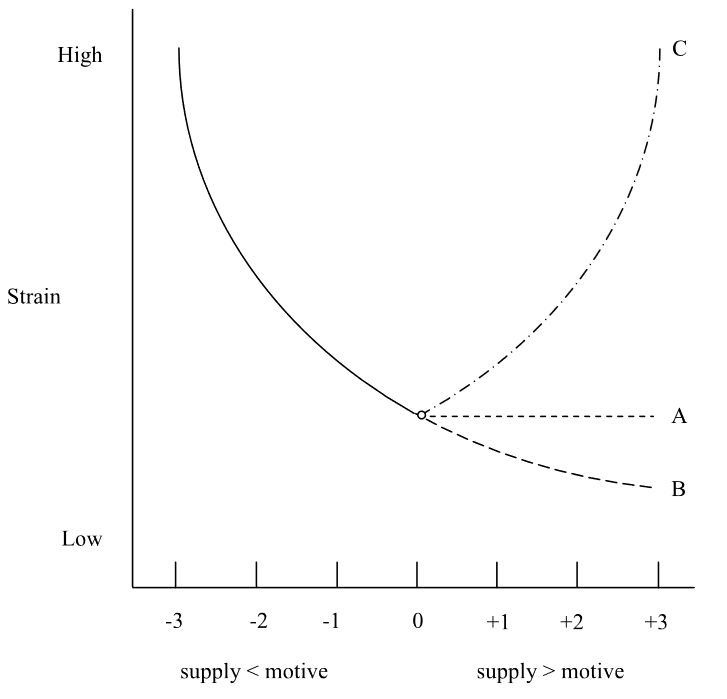
\includegraphics[width=0.75\textwidth]{gfx/ueberschuss_supply_motive.png}
	\caption[Auswirkungen eines Bedürfnisse-Angebote Misfits]{Auswirkungen eines Bedürfnisse-Angebote Misfits\\(Eigene Darstellung in Anlehnung an \cite[S. 23]{edwards:2008})}
	\label{fig:personEnvironmentFit:auswirkungenErhoehterAngebote:abb1}
\end{figure}

Die durchgezogene Linie auf der linken Hälfte von Abbildung \ref{fig:personEnvironmentFit:auswirkungenErhoehterAngebote:abb1} verdeutlicht, dass die mentale Belastung eines Individuums umso stärker zunimmt, je weniger dessen Bedürfnisse erfüllt werden \cite[S. 30]{mechanismsOfJobStressAndStrain:1982}. Der Verlauf dieser Kurve kann über die in Gleichung \ref{fig:personEnvironmentFit:auswirkungenErhoehterAngebote:formel1} dargestellte algebraische Differenzberechnung bestimmt werden \cite[S. 2]{edwards:1993}.
\begin{equation}
	B = P - E
	\label{fig:personEnvironmentFit:auswirkungenErhoehterAngebote:formel1}
\end{equation}
Alternativ bietet sich die Verwendung der quadrierten Differenz aus Gleichung \ref{fig:personEnvironmentFit:auswirkungenErhoehterAngebote:formel3} an \cite[S. 2]{edwards:1993}.
\begin{equation}
	B = (P - E)^2
	\label{fig:personEnvironmentFit:auswirkungenErhoehterAngebote:formel3}
\end{equation}
In den Gleichungen \ref{fig:personEnvironmentFit:auswirkungenErhoehterAngebote:formel1} und \ref{fig:personEnvironmentFit:auswirkungenErhoehterAngebote:formel3} steht $B$ für die mentale Belastung des Mitarbeiters. $P$ stellt die von einer Person gewünschte Menge eines bestimmten Wertes dar. Die vom Mitarbeiter wahrgenommene erhaltene Menge des entsprechenden Wertes seitens der Umgebung wird über Parameter $E$ ausgedrückt \cite[S. 2]{edwards:1993}.

Übersteigen die Angebote der Umgebung die Bedürfnisse der Person, mündet dies in einer der drei gepunkteten Linien A, B oder C in Abbildung \ref{fig:personEnvironmentFit:auswirkungenErhoehterAngebote:abb1} \cite[S. 29ff.]{mechanismsOfJobStressAndStrain:1982}. Kurve A zeigt einen monotonen Verlauf der mentalen Belastung. Dieser entsteht, wenn eine Person die Übererfüllung eines Bedürfnisses entweder für einen späteren Zeitpunkt aufsparen oder in die Befriedigung verwandter Motive investieren kann \cite[S. 30]{mechanismsOfJobStressAndStrain:1982}\cite[S. 11]{harrison:1978}. Dieser Sachverhalt ist laut \textcite[S. 21]{edwards:2008} beispielsweise erfüllt, wenn einer Person mehr Gehalt zusteht, als diese für die Zahlung ihrer Lebenskosten benötigt. Dem Forscher zu Folge könnte das überschüssige Geld entweder für die Zahlung von Lebenshaltungskosten in den Folgemonaten aufgespart oder zusätzlich in das mögliche Bedürfnis nach Luxusgütern investiert werden. Für die Berechnung von Kurve A kann ebenfalls Gleichung \ref{fig:personEnvironmentFit:auswirkungenErhoehterAngebote:formel1} verwendet werden \cite[S. 2]{edwards:1993}.

Linie B hat den Verlauf einer quadratischen Funktion und tritt ein, wenn die Übererfüllung eines Bedürfnisses entweder die Befriedigung dieses oder eines verwandten Motivs hemmt \cite[S. 5]{caplan:1987}. \textcite[S. 12]{harrison:1978} nannte hierfür das Bedürfnis einer Person nach sozialem Austausch als Beispiel, welches bei Übererfüllung das Verlangen nach Privatsphäre verletzt. Der Verlauf von Kurve B kann über Gleichung \ref{fig:personEnvironmentFit:auswirkungenErhoehterAngebote:formel3} oder die in Gleichung \ref{fig:personEnvironmentFit:auswirkungenErhoehterAngebote:formel2} dargestellte absolute Differenzberechnung bestimmt werden \cite[S. 2]{edwards:1993}.
\begin{equation}
	B = |P - E|
	\label{fig:personEnvironmentFit:auswirkungenErhoehterAngebote:formel2}
\end{equation}
Kurve C stellt eine asymptotische Beziehung zur mentalen Belastung dar. Sie tritt ein, wenn weder die Bedingungen von Kurve A noch von Linie B zutreffen. Eine Übererfüllung des Bedürfnisses hat folglich weder positive noch negative Auswirkungen auf die Person \cite[S. 30]{mechanismsOfJobStressAndStrain:1982}. Ein Beispiel für eine solche Beziehung ist ein Überangebot an Parkplätzen beim Arbeitgeber. Da der Mitarbeiter nur ein Fahrzeug besitzt, kann dieser von zusätzlichen Angeboten keinen Gebrauch machen und diese auch nicht für einen späteren Zeitpunkt aufsparen. Die zusätzlichen Parkplätze schaden auch keinem anderen Bedürfnis des Mitarbeiters. Somit entstehen weder positive noch negative Auswirkungen auf dessen Wohlbefinden. Zur Bestimmung von Kurve C wird die Belastung gleich dem Wert null gesetzt. Dieses Vorgehen ist in Gleichung \ref{fig:personEnvironmentFit:auswirkungenErhoehterAngebote:formel4} dargestellt \cite[S. 2]{edwards:1993}.
\begin{equation}
	B = 0
	\label{fig:personEnvironmentFit:auswirkungenErhoehterAngebote:formel4}
\end{equation}
Verschiedene Autoren gehen davon aus, dass die Beziehungen aus Abbildung \ref{fig:personEnvironmentFit:auswirkungenErhoehterAngebote:abb1} auch für den Anforderungen-Fähigkeiten Fit zu erwarten sind. Dies gilt gemäß der Erkenntnisse aus Kapitel \ref{ch:personEnvironmentFit:subjektivObjektiv} nur, wenn das Erfüllen der Anforderungen Auswirkungen auf die inneren Werte des Mitarbeiters hat \cite[S. 12f.]{harrison:1978}. Wie an der durchgezogenen Linie auf der linken Seite von Abbildung \ref{fig:personEnvironmentFit:auswirkungenErhoehterAngebote:abb1} zu erkennen, entsteht in jedem Fall psychische Belastung, wenn die Anforderungen der Umgebung die Kenntnisse des Mitarbeiters übersteigen \cite[S. 5]{schuler:1980}. Sind dagegen die Fähigkeiten des Angestellten stärker ausgeprägt als erforderlich, resultiert dies in einer der Kurven A bis C. Linie A tritt ein, wenn der Mitarbeiter seine gewonnenen Freiräume nutzen kann, um verwandte Bedürfnisse zu erfüllen. Schaden die zu niedrigen Anforderungen einem Bedürfnis des Angestellten, entsteht Kurve B. Haben die zu hohen Fähigkeiten des Mitarbeiters weder positive noch negative Auswirkungen auf dessen Wohlbefinden, resultiert Linie C \cite[S. 22f.]{edwards:2008}.

Unterschiedliche Publikationen stellten fest, dass der Verlauf der Kurven nicht alleine von den Auswirkungen der Misfits auf die Motive des Mitarbeiters abhängig ist. Zusätzlich muss beachtet werden, als wie wichtig der Angestellte die betroffenen Bedürfnisse bewertet \cite[S. 9f.]{edwards:1996}. 

\section{Einbeziehung der Wichtigkeiten von Bedürfnissen}
\label{ch:personEnvironmentFit:wichtigkeiten}
%Bereits  \textcite[S. 7]{copingAndAdaption:1974} empfahlen die Einbeziehung von Wichtigkeitswerten in die Berechnung des \acp{PEFit}. Auf welche Weise diese Werte einbezogen werden sollten, ließen die Autoren zum damaligen Zeitpunkt jedoch unbeantwortet \cite[S. 19]{edwards:2008}.
\textcite[S. 38]{harrison:1985} schlug vor, den \ac{PEFit} für jede untersuchte Variable einzeln zu berechnen und die Ergebnisse jeweils mit einem subjektiven Wichtigkeitswert zu multiplizieren. Diese Einschätzung teilte auch \textcite[S. 18]{locke:1969}\cite[S. 8f.]{locke:1976}. Er gilt als einer der einflussreichsten Wissenschaftler auf dem Gebiet der Arbeitszufriedenheit \cite[S. 12]{edwards:2008}. Diese kann laut \textcite[S. 8]{locke:1969} nur entstehen, wenn Mitarbeiter das Gefühl haben, für sie als wichtig erachtete Werte durch ihre Tätigkeit zu erfüllen. Aus diesem Grund empfahl er zur Berechnung der Arbeitszufriedenheit eines Angestellten zwei Kennzahlen heranzuziehen: Die Differenz aus wahrgenommener und gewünschter Menge eines Wertes und die subjektive Wichtigkeit des Motivs \cite[S. 8]{locke:1976}. \textcite[S. 16]{locke:1969} betonte, dass je nach untersuchtem Wert unterschiedliche Berechnungen wie algebraische oder absolute Differenz angewendet werden können. Ein Beispiel für eine Multiplikation mit algebraischer Differenz ist in folgender Gleichung \ref{fig:personEnvironmentFit:wichtigkeiten:formel1} dargestellt \cite[S. 9]{edwards:1990}.
\begin{equation}
	Y = b * (P - E)
	\label{fig:personEnvironmentFit:wichtigkeiten:formel1}
\end{equation}
In Gleichung \ref{fig:personEnvironmentFit:wichtigkeiten:formel1} steht $Y$ für das untersuchte Ergebnis wie beispielsweise die Arbeitszufriedenheit. $b$ stellt den subjektiven Wichtigkeitswert dar. Dieser wird mit der Differenz aus gewünschter Menge eines Wertes einer Person $P$ und wahrgenommener Menge des Wertes der Umgebung $E$ multipliziert \cite[S. 9f.]{edwards:1990}.
\newpage
Derartige Multiplikationen mit einem Differenzwert haben zur Folge, dass die in Abbildung \ref{fig:personEnvironmentFit:auswirkungenErhoehterAngebote:abb1} dargestellten Kurven mit steigender Wichtigkeit steiler werden \cite[S. 9]{locke:1976}. Abbildung \ref{fig:personEnvironmentFit:wichtigkeiten:abb1} verdeutlicht die entstehenden Stauchungen durch Wichtigkeitswerte.

\begin{figure}[h]
	\centering
	
	\subfloat[Algebraische Differenz]{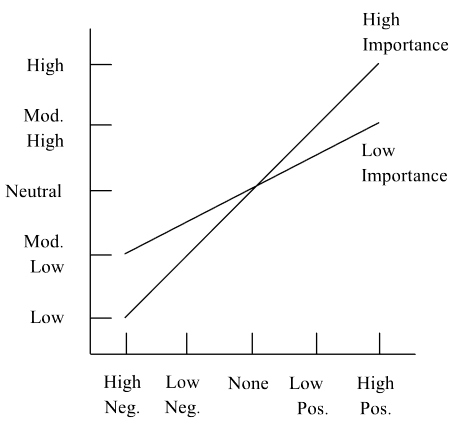
\includegraphics[width = 0.5\textwidth]{gfx/Locke-A.png}}
	\subfloat[Absolute Differenz]{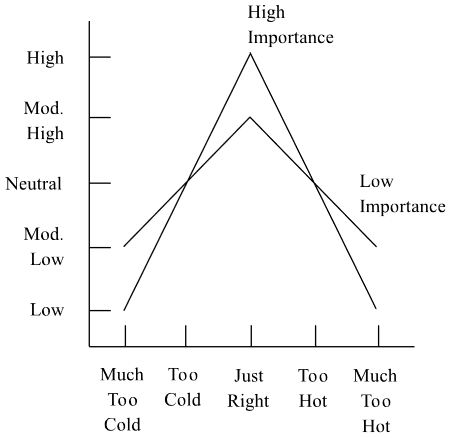
\includegraphics[width = 0.5\textwidth]{gfx/Locke-B.png}}
	
	\caption[Stauchung von Funktionsgraphen durch Wichtigkeiten]{Stauchung von Funktionsgraphen durch Wichtigkeiten\\
	(Eigene Darstellung in Anlehnung an \cite[S. 1305]{locke:1976})}
	%(Aus \cite[S. 13f.]{edwards:2008}, nach \cite[S. 1305]{locke:1976})
	\label{fig:personEnvironmentFit:wichtigkeiten:abb1}
\end{figure}

Im linken Teil (a) von Abbildung \ref{fig:personEnvironmentFit:wichtigkeiten:abb1} ist eine monotone Funktion basierend auf einer algebraischen Differenzberechnung dargestellt. Die rechte Seite der Grafik (b) zeigt den Verlauf einer Berechnung mit absoluter Differenz. In beiden Darstellungen ist zu erkennen, dass die Kurven bei fehlender Wichtigkeit ausschließlich im mittleren Bereich verlaufen. Ist einem Individuum das jeweilige Bedürfnis dagegen wichtig, füllt die Kurve den gesamten verfügbaren Bereich von niedrig bis hoch. Dieses Vorgehen führt zur Stauchung der Funktionsgraphen und damit zu einem stärkeren Ansteigen bzw. Absinken der Belastung des Individuums. 

Derartige Berechnungen kritisierte \textcite[S. 51ff.]{edwards:1991}\cite[S. 9ff.]{edwards:1990}\cite[S. 2ff.]{edwards:1993}\cite[S. 2ff.]{edwards:1993b} in mehreren seiner Arbeiten. Dabei diskutierte er insbesondere die Multiplikation mit dem Differenzwert. Er ist der Auffassung, dass die aus der Differenzberechnung resultierenden zweidimensionalen Grafiken die Komplexität eines \acp{PEFit} nicht vollständig abbilden. Deshalb empfahl er, die Berechnungen mittels Regressionsgleichungen durchzuführen.%TODO: Quelle

\section{Anwendung von Regressionsgleichungen}
\label{ch:personEnvironmentFit:regressionsgleichungen}
\textcite[S. 51ff.]{edwards:1991}\cite[S. 9ff.]{edwards:1990}\cite[S. 2ff.]{edwards:1993}\cite[S. 2ff.]{edwards:1993b} empfahl, die Multiplikationen separat für jeden Wert von Person und Umgebung durchzuführen. Formel \ref{fig:personEnvironmentFit:wichtigkeiten:formel1} könnte hierfür zu folgender Regressionsgleichung \ref{fig:personEnvironmentFit:wichtigkeiten:formel2} umgestellt werden \cite[S. 9f.]{edwards:1990}\cite[S. 2f.]{edwards:1993b}.
\begin{equation}
	Y = b_1 * P - b_2 * E + a
	\label{fig:personEnvironmentFit:wichtigkeiten:formel2}
\end{equation}
Die Koeffizienten $b_1$ und $b_2$ stehen in Gleichung \ref{fig:personEnvironmentFit:wichtigkeiten:formel2} für die separaten Wichtigkeiten von gewünschter ($P$) und wahrgenommener Menge ($E$) eines Wertes. Durch diese Art der Berechnung entstehen aus zweidimensionalen Grafiken dreidimensionale Modelle \cite[S. 2]{edwards:1993}. Solche Darstellungen sind dem Wissenschaftler zu Folge besser geeignet, Ungleichmäßigkeiten in den Oberflächen abzubilden \cite[S. 51ff.]{edwards:1991}. So stellte \textcite[S. 53ff.]{edwards:1991} beispielsweise bei der Datenanalyse einer Studie mit mehreren hundert Teilnehmern die in Abbildung \ref{fig:personEnvironmentFit:wichtigkeiten:abb2} dargestellte dreidimensionale Beziehung von \ac{PEFit} und Zufriedenheit fest.

\begin{figure}[h]
	\centering
	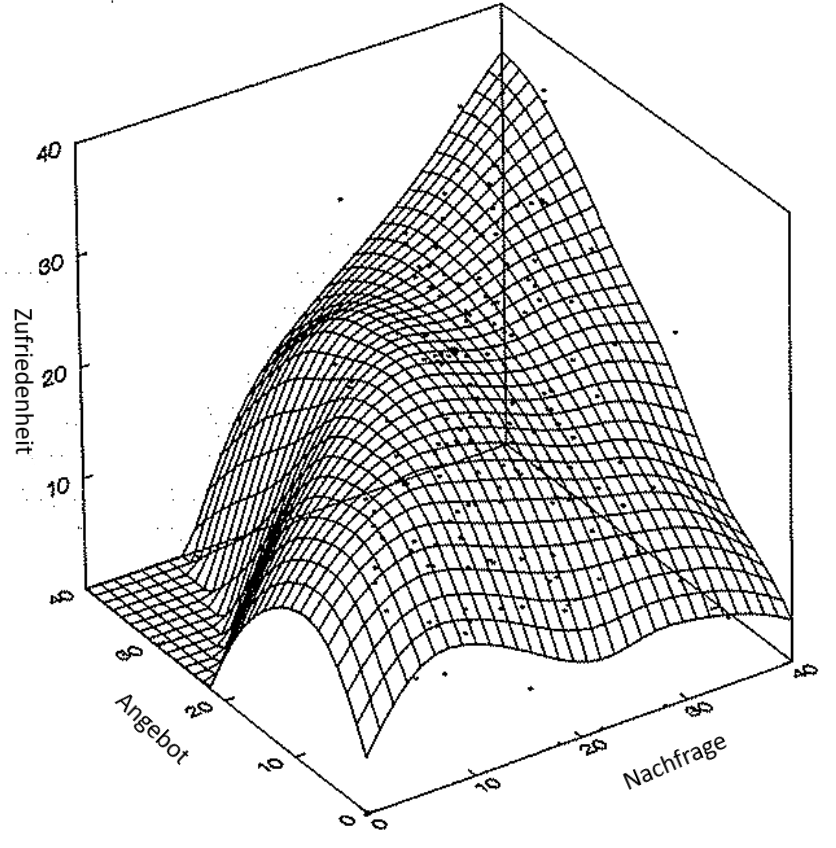
\includegraphics[width=0.8\textwidth]{gfx/drei_d_modell.png}
	\caption[Dreidimensionale Beziehung von P-E Fit und Zufriedenheit]{Dreidimensionale Beziehung von P-E Fit und Zufriedenheit\\
	(Eigene Darstellung in Anlehnung an \cite[S. 57]{edwards:1991})}
	\label{fig:personEnvironmentFit:wichtigkeiten:abb2}
\end{figure}

Um die stärkere Aussagekraft der Regressionsgleichungen zu untermauern, werteten \textcite[S. 18ff.]{edwards:1993b} einen umfangreichen Datensatz von \textcite[S. 9ff.]{mechanismsOfJobStressAndStrain:1982} erneut aus. Dabei gelang es ihnen, durch Anwendung von Regressionsgleichungen im Vergleich zur erstmaligen Untersuchung einen wesentlich höheren Anteil an Varianz zu erklären \cite[S. 8]{su:2015}.
\shorthandon{"}

\definecolor{exxetagray}{gray}{0.75}
\definecolor{itemcolor}{RGB}{179,217,255}
\definecolor{usercolor}{RGB}{255,204,179}

\shorthandoff{"}
\chapter{Empfehlungssysteme}
\label{ch:empfehlungssysteme}

\section{Einführung}
\label{ch:empfehlungssysteme:einfuehrung}
Der Begriff des Empfehlungssystems ist im englischsprachigen Raum auch unter Bezeichnungen wie Recommender System \cite[S. 1]{lu:2015}, Recommender Engine \cite[S. 1]{panigrahi:2016} und Recommendation System \cite[S. 1]{ebesu:2018} verbreitet. Er wurde erstmals im Jahr 1997 von \textcite[S. 1]{resnick:1997} geprägt. Dass der Begriff gerade zu diesem Zeitpunkt entstand, ist auf die zur damaligen Zeit stark wachsende Internetnutzung und die damit verbundenen einfachen Möglichkeiten zur Sammlung und Auswertung großer Mengen an Nutzerdaten zurückzuführen \cite[S. xvii]{recommenderSystems:2016}.

Heutzutage sind insbesondere große IT-Konzerne wie Amazon, Facebook, Google und Netflix bekannt für den Einsatz von Empfehlungssystemen \cite[S. 1]{zarzour:2018}. Diese Unternehmen nutzen Recommender Engines, um ihren Kunden personalisierte Vorschläge zu den Inhalten ihrer Plattformen anzuzeigen \cite[S. 2]{jeckmans:2013}. Häufig entfällt dabei für den Anwender vollständig die Notwendigkeit einer manuellen Suche \cite[S. 1]{comibingCareer:2013}.

Der Einsatz von Empfehlungssystemen wird in der Literatur kritisch diskutiert. Beispielsweise beobachteten \textcite[S. 17f.]{alfano:2020}, dass das Empfehlungssystem der Videostreaming-Plattform YouTube dazu tendiert, neuen Anwendern zur Verlängerung ihrer Nutzungszeit verschwörungstheoretische Inhalte auszuspielen. Eine Untersuchung von Forschern des sozialen Netzwerks Facebook kam zu dem Ergebnis, dass deren Recommender Engine Nutzern verstärkt Inhalte präsentiert, welche konform mit deren Ideologien sind \cite[S. 2]{bakshy:2015}. \textcite[S. 1ff.]{pariser:2012} prägte für diese Art der Personalisierung den Begriff der Filterblase.

Empfehlungssysteme haben aber auch einen bedeutenden Anteil am wirtschaftlichen Erfolg großer Internetplattformen. So führten beispielsweise \textcite[S. 6f.]{sharma:2015} in einer Studie aus den Jahren 2013 und 2014 etwa 30 Prozent der Seitenaufrufe beim Online-Händler Amazon unmittelbar auf den Einsatz von Empfehlungssystemen zurück. \textcite[S. 5]{gomezuribe:2016} stellten bei einer Analyse der Streaming-Plattform Netflix fest, dass ca. 80 Prozent der Nutzungszeit auf Videos entfiel, welche Nutzern ohne vorherige Suche von einer Recommender Engine angezeigt wurden.

Um solche Vorschläge generieren zu können, suchen Empfehlungssysteme relevante Inhalte basierend auf den Präferenzen der Anwender aus \cite[S. 1]{das:2017}. Zu diesem Zweck müssen benötigte Nutzerdaten zunächst erhoben und in einer maschinell auswertbaren Struktur gespeichert werden.

\section{Zugrundeliegende Datenstruktur}
\label{ch:empfehlungssysteme:arbeitsweise}
Empfehlungssysteme können die Präferenzen ihrer Nutzer sowohl über explizite als auch implizite Rückmeldungen erfassen. Explizites Feedback erhalten Plattformen beispielsweise über abgegebene Produktbewertungen oder "Gefällt mir"-Angaben in sozialen Netzwerken. Um implizite Rückmeldungen auszuwerten, werden häufig Verhaltensweisen der Nutzer aufgezeichnet. Hierbei kann es sich beispielsweise um Suchverläufe oder die Wiedergabedauer von Videos handeln \cite[S. 3]{pu:2012}.

Das gesammelte Feedback überführen Analysten in die Struktur von Matrizen \cite[S. 11f.]{recommenderSystems:2016}. Ein Beispiel für eine Matrix mit explizit erfassten Bewertungen der Fähigkeiten von Mitarbeitern ist in Tabelle \ref{tbl:empfehlungssysteme:arbeitsweise:tbl1} dargestellt.

\begin{table}[h]
	\centering
	\begin{tabular}{c|c|c|c|c|c|c}
	 & \textbf{Java} & \textbf{Python} & \textbf{MySQL} & \textbf{MongoDB} & \textbf{HDFS} & \textbf{Spark}\\ 
	\hline
	\textbf{Doe, Jane}     & ? & 4 & 3 & 3 & ? & ?\\
	\textbf{Doe, John}     & 3 & ? & 2 & ? & 1 & ?\\
	\textbf{Muster, Erika} & ? & ? & ? & ? & 5 & 3\\
	\textbf{Muster, Max}   & 2 & 3 & 1 & ? & ? & ?
	\end{tabular}
	\caption{Beispiel für die Matrixdarstellung von Fähigkeiten}
	\label{tbl:empfehlungssysteme:arbeitsweise:tbl1}
\end{table}

In Tabelle \ref{tbl:empfehlungssysteme:arbeitsweise:tbl1} sind in der ersten Spalte die Mitarbeiter eines Unternehmens gespeichert. Diese werden als Nutzer bezeichnet. In den Kopfzeilen der folgenden Spalten sind verschiedene Fähigkeiten eingetragen. Diese werden Elemente genannt. In der Mitte der Tabelle befinden sich die Bewertungen der Fähigkeiten jedes Nutzers \cite[S. 1f.]{strub:2016}. Im Beispiel aus Tabelle \ref{tbl:empfehlungssysteme:arbeitsweise:tbl1} wurden die expliziten Beurteilungen auf einer Skala von eins bis fünf vergeben. Diese bewerteten Matrix-Einträge werden  als beobachtet oder spezifiziert bezeichnet. Unbewertete Elemente sind mit einem Fragezeichen gekennzeichnet und werden unbeobachtet oder fehlend genannt \cite[S. 8]{recommenderSystems:2016}.

Zahlreiche Wissenschaftler in der Literatur sind sich einig, dass für die Empfehlung geeigneter Kandidaten für eine Stelle bzw. Projektposition ein einfacher Abgleich zwischen gesuchten und vorhandenen Fähigkeiten in der Matrix eine unzureichende Lösung darstellt \cite[S. 1]{enhancingERecruitment:2012}\cite[S. 1]{faerber:2003}\cite[S. 2]{prospect:2010} und der Komplexität der Aufgabe nicht gerecht wird \cite[S. 1]{malinowski:2008}. So kritisierten beispielsweise \textcite[S. 1f.]{mitre:2014}, dass bei einem solchen Ansatz Synonyme und verwandte Fähigkeit nicht in die Suche einbezogen werden. Um diesem Problem zu begegnen, existieren in der Literatur unterschiedliche Ansätze, Recommender Engines zu implementieren. Ein verbreitetes Verfahren ist das kollaborative Filtern.

\section{Kollaboratives Filtern}
\label{ch:empfehlungssysteme:cf}
Ein Ziel von Verfahren im Bereich des kollaborativen Filterns ist das Vorhersagen unbewerteter Einträge in Tabelle \ref{tbl:empfehlungssysteme:arbeitsweise:tbl1}. Unbeobachtete Werte eines Zielnutzers werden dabei über Ähnlichkeitsberechnungen aus vergebenen Beurteilungen anderer Anwender geschlussfolgert \cite[S. 1]{su:2009}.

\textcite[S. 3]{breese:1998} unterschieden zwischen speicher- und modellbasierten Algorithmen. Speicherbasierte Verfahren übertragen sämtliche Nutzer und deren Bewertungen bei der Berechnung von Empfehlungen vollständig in den Hauptspeicher des Rechners. Modellbasierte Verfahren nutzen dagegen Algorithmen aus dem Bereich des Data Minings. Diese werden verwendet, um vor dem Einsatz in der Produktivumgebung statistische Vorhersagemodelle zu entwickeln \cite[S. 3]{breese:1998}\cite[S. 11]{schafer:2007}. Im Folgenden werden unterschiedliche Ansätze vorgestellt, speicher- und modellbasierte Verfahren zu implementieren.

\subsection{Speicherbasierte Verfahren}
\label{ch:empfehlungssysteme:cf:speicherbasiert}
Bei der Entwicklung speicherbasierter Verfahren kommen nachbarschaftsbasierte Algorithmen zum Einsatz \cite[S. 29]{recommenderSystems:2016}. Soll beispielsweise die fehlende Java-Bewertung von Jane Doe in Tabelle \ref{tbl:empfehlungssysteme:arbeitsweise:tbl1} vorhergesagt werden, erfolgt dies über paarweise Ähnlichkeitsberechnungen \cite[S. 2f.]{bharti:2019}. Verwenden Algorithmen dabei die Ähnlichkeiten zwischen Mitarbeitern bzw. Tabellenzeilen zur Vorhersage, werden diese als nutzerorientiert bezeichnet. Greifen Verfahren dagegen auf die Gleichartigkeit zwischen Fähigkeiten bzw. Tabellenspalten zurück, werden sie elementorientiert genannt \cite[S. 1f.]{duong:2018}. Laut \textcite[S. 42]{recommenderSystems:2016} liefern elementorientierte Verfahren häufig präzisere, nutzerorientierte Methoden dafür diversere Ergebnisse. Somit erwartet der Autor, dass die Vorschläge der elementorientierten Ansätze für den Nutzer relevanter erscheinen. Jedoch bemängelte er das hohe Risiko bei diesen Verfahren, dass dem Anwender aufgrund der starken Ähnlichkeit der Elemente entweder alle Vorschläge zusagen oder kein einziger.

Bei der Implementierung nachbarschaftsbasierter Verfahren kommen häufig \ac{KNN}-Algorithmen zum Einsatz \cite[S. 1]{nayak:2018}. Um diese zur Vorhersage der Java-Bewertung von Jane Doe anzuwenden, wird bei elementorientierten Verfahren die Ähnlichkeit zwischen Java und jeder anderen Fähigkeit bestimmt, welche Jane Doe beherrscht. Anschließend wird die durchschnittliche Bewertung der k-ähnlichsten Fähigkeiten berechnet und als Java-Beurteilung für Jane Doe eingesetzt \cite[S. 2]{hao:2013} Welcher Wert für k verwendet werden sollte, kann pauschal nicht beantwortet werden. Beispielsweise ist es möglich, Verfahren aus dem Bereich des maschinellen Lernens zu nutzen, um abhängig von den vorhandenen Daten einen geeigneten Wert für k zu ermitteln \cite[S. 2f.]{jiang:2007}.

Bei nutzerorientierten Algorithmen wird die Gleichartigkeit zwischen Jane Doe und allen anderen Mitarbeitern berechnet. Daraufhin wird die durchschnittliche Java-Beurteilung der k-ähnlichsten Mitarbeiter bestimmt und als Java-Bewertung für Jane Doe vorhergesagt \cite[S. 2f.]{hao:2013}.

Zur Ähnlichkeitsberechnung können unterschiedliche Algorithmen wie die Jaccard-Ähnlichkeit \cite[S. 2]{bharti:2019}, die euklidische Distanz \cite[S. 3]{cheng:2013} oder die Kosinus-Ähnlichkeit \cite[S. 2]{duong:2018} verwendet werden. Beispielhaft ist in der folgenden Gleichung \ref{fig:empfehlungssysteme:cf:speicherbasiert:formel1} die Formel zur Berechnung der Kosinus-Ähnlichkeit zwischen zwei Vektoren A und B dargestellt \cite[S. 111]{bharti:2019}.
\begin{equation}
cos(A,B) = \frac{(\vec{A} * \vec{B})}{|\vec{A}| * |\vec{B}|} = \frac{\sum_{i=1}^n A_i * B_i}{\sqrt{\sum_{i=1}^n (A_i)^2} * \sqrt{\sum_{i=1}^n (B_i)^2}}
\label{fig:empfehlungssysteme:cf:speicherbasiert:formel1}
\end{equation}
Anstelle der Vektoren A und B können in Gleichung \ref{fig:empfehlungssysteme:cf:speicherbasiert:formel1} paarweise die Spalten/Fähigkeiten bzw. Zeilen/Mitarbeiter aus Tabelle \ref{tbl:empfehlungssysteme:arbeitsweise:tbl1} eingesetzt werden.

Gleichung \ref{fig:empfehlungssysteme:cf:speicherbasiert:formel2} zeigt die nutzerbasierte Ähnlichkeitsberechnung zwischen Jane Doe und Max Muster anhand der Daten aus Tabelle \ref{tbl:empfehlungssysteme:arbeitsweise:tbl1}. Dort ist zu erkennen, dass ausschließlich Tabellenspalten in die Berechnung einbezogen werden, welche beide Mitarbeiter bewertet haben \cite[S. 2f.]{hao:2013}.
\begin{equation}
	cos(Jane Doe,Max Muster) = \frac{(4*3 + 3*1)}{\sqrt{4^2 + 3^2} * \sqrt{3^2 + 1^2}} \approx \frac{15}{15,811} \approx 0,95
	\label{fig:empfehlungssysteme:cf:speicherbasiert:formel2}
\end{equation}
Wie in der folgenden Gleichung \ref{fig:empfehlungssysteme:cf:speicherbasiert:formel3} dargestellt, kann analog auch die elementbasierte Ähnlichkeit für Java und MySQL aus Tabelle \ref{tbl:empfehlungssysteme:arbeitsweise:tbl1} mittels Kosinus-Distanz berechnet werden.
\begin{equation}
	cos(Java, MySQL) = \frac{(3*2 + 2*1)}{\sqrt{3^2 + 2^2} * \sqrt{2^2 + 1^2}} \approx \frac{8}{8,063} \approx 0,992
	\label{fig:empfehlungssysteme:cf:speicherbasiert:formel3}
\end{equation}
In den Gleichungen \ref{fig:empfehlungssysteme:cf:speicherbasiert:formel2} und \ref{fig:empfehlungssysteme:cf:speicherbasiert:formel3} ist zu erkennen, dass im vorliegenden Beispiel eine Ähnlichkeit zwischen Jane Doe und Max Muster von 95 Prozent und eine Gleichartigkeit von 99,2 Prozent zwischen Java und MySQL besteht.%Um über nutzerbasiertes kollaboratives Filtern die Java-Bewertung von Jane Doe vorherzusagen, müsste zusätzlich die Ähnlichkeit zwischen Jane Doe und allen anderen Nutzern in der Datenbank bestimmt werden. Anschließend könnte das Empfehlungssystem die k ähnlichsten Nutzer zu Jane Doe auswählen und deren durchschnittliche Java-Bewertung als Fähigkeitseinschätzung bei Jane Doe einsetzen. 

\textcite[S. 35ff.]{recommenderSystems:2016} kritisierte an solchen Ähnlichkeitsberechnungen, dass möglicher Bias die Ergebnisse verzerren kann. So könnten einzelne Mitarbeiter ihre Fähigkeiten grundsätzlich schlechter oder besser einschätzen als andere Angestellte. Aus diesem Grund empfahl der Autor, vor den Ähnlichkeitsberechnungen zunächst eine Mittelwert-Zentrierung auszuführen. Hierbei wird in Tabelle \ref{tbl:empfehlungssysteme:arbeitsweise:tbl1} die durchschnittliche Bewertung jedes Nutzers bestimmt und von dessen vorhandenen Beurteilungen abgezogen. Dabei entstehende negative Bewertungen müssen anschließend aus der Tabelle entfernt werden. Dieses Vorgehen ist in der Literatur auch unter der Bezeichnung Pearson Korrelation bekannt \cite[S. 3]{bharti:2019}.

Es gilt zu beachten, dass die bisher vorgestellten Algorithmen im Bereich des speicherbasierten kollaborativen Filterns anfällig für das Sparsity Problem sind \cite[S. 3f.]{grvcar:2006}. Dieses bezeichnet das Phänomen, dass in der Praxis meist für einen Bruchteil aller Spalten sehr viele Bewertungen und für einen Großteil der Elemente nur sehr wenige Beurteilungen vorliegen \cite[S. 8]{recommenderSystems:2016}. So stellten beispielsweise \textcite[S. 3]{mitre:2014} bei der Implementierung ihres Projekt-Empfehlungssystems fest, dass über die Hälfte der ca. 17.000 vergebenen Fähigkeiten von nur je einem Mitarbeiter angegeben wurden.
Für diese Häufigkeitsverteilung prägte \textcite[S. 12]{anderson:2007} den Begriff des langen (Ratten-)Schwanzes (Long Tail). Erkennbar wird dieser, wenn Bewertungen, wie in Abbildung \ref{fig:empfehlungssysteme:cf:speicherbasiert:abb1} dargestellt, in Form eines Diagramms aggregiert werden.

\begin{figure}[h]
	\centering
	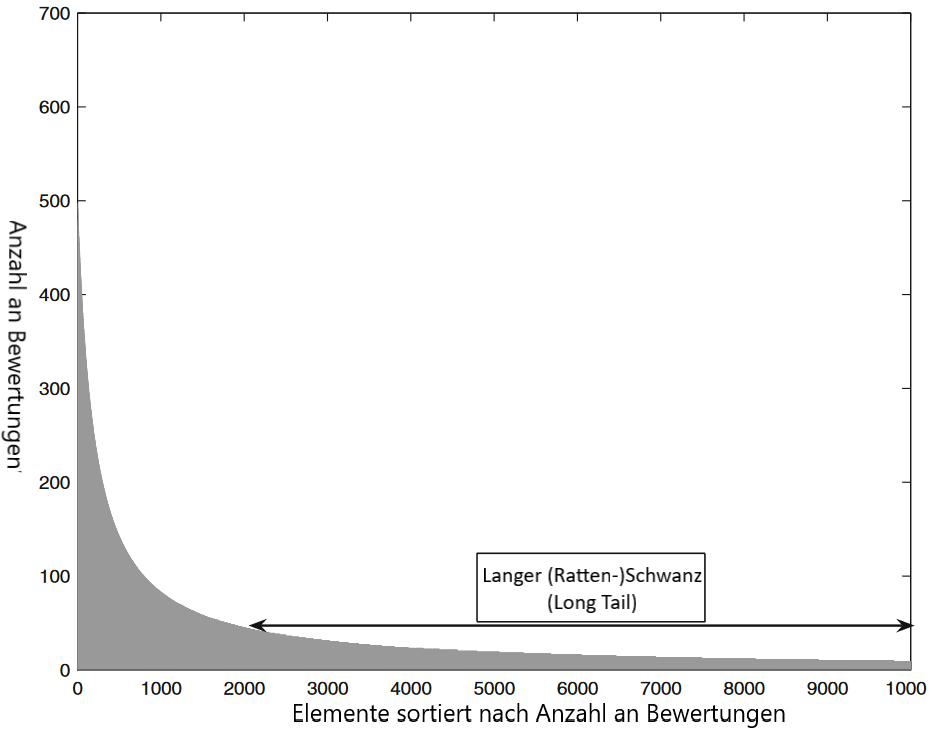
\includegraphics[width=1\textwidth]{gfx/long-tail.png}
	\caption[Darstellung des langen (Ratten-)Schwanzes]{Darstellung des langen (Ratten-)Schwanzes\\
		(Eigene Darstellung in Anlehnung an \cite[S. 33]{recommenderSystems:2016})}
	\label{fig:empfehlungssysteme:cf:speicherbasiert:abb1}
\end{figure}

Die in Abbildung \ref{fig:empfehlungssysteme:cf:speicherbasiert:abb1} dargestellte Häufigkeitsverteilung von abgegebenen Bewertungen spiegelt \textcite[S. 1ff.]{anderson:2007} zu Folge einen allgemeinen Trend wider, welchen er im Zusammenhang mit der Digitalisierung beobachtet. Der Autor stellte fest, dass sich Menschen aufgrund der heute verfügbaren breiten Angebote wesentlich diverser orientieren, als es vor einigen Jahrzehnten der Fall war \cite[S. 1ff.]{anderson:2007}.

Das Sparsity Problem kann auch in Tabelle \ref{tbl:empfehlungssysteme:arbeitsweise:tbl1} beobachtet werden. Dort haben MongoDB und Spark jeweils nur eine Bewertung. Für diese Fähigkeiten ist es über Ähnlichkeitsberechnungen im Bereich des speicherbasierten kollaborativen Filterns somit nicht möglich, für alle Angestellten robuste Vorhersagen zu ermitteln.

Um diesem Problem zu begegnen, kann die bisher verwendete Matrixdarstellung in die Form eines bipartiten Graphen überführt werden \cite[S. 2f.]{huang:2004}. Diese Datenstruktur zeichnet sich durch die Verwendung zwei unterschiedlicher Arten von Knoten zur separaten Speicherung von Nutzern und Elementen aus. Bewertungen werden bei dieser Darstellungsform über gewichtete Kanten im Graphen dargestellt \cite[S. 1f.]{cao:2021}.

Abbildung \ref{fig:empfehlungssysteme:cf:speicherbasiert:abb2} zeigt die Fähigkeitsmatrix aus Tabelle \ref{tbl:empfehlungssysteme:arbeitsweise:tbl1} in der Datenstruktur eines bipartiten Graphen. In der Darstellung sind die Knoten der Mitarbeiter rot und die Knoten der Fähigkeiten blau markiert.

\begin{figure}[h]
	\centering	
	\begin{tikzpicture}[node distance={32mm}, thick, main/.style = {draw, circle}] 
		\node[main, fill=itemcolor] (MongoDB) {$MongoDB$}; 
		\node[main, fill=itemcolor] (Python) [below right of=MongoDB] {$Python$}; 
		\node[main, fill=itemcolor] (MySQL) [above right of=Python] {$MySQL$}; 
		\node[main, fill=itemcolor] (Java) [below right of=MySQL] {$Java$}; 
		\node[main, fill=itemcolor] (HDFS) [above right of=Java] {$HDFS$}; 
		\node[main, fill=itemcolor] (Spark) [below right of=HDFS] {$Spark$};
		
		\node[main, fill=usercolor] (Jane) [above right of=MongoDB] {$Jane D.$}; 
		\node[main, fill=usercolor] (John) [above left of=HDFS] {$John D.$}; 
		\node[main, fill=usercolor] (Max) [below of=MySQL] {$Max M.$};
		\node[main, fill=usercolor] (Erika) [above right of=HDFS] {$Erika M.$}; 
		
		\draw (Jane) -- node[midway, right] {4} (Python);
		\draw (Jane) -- node[midway, above] {3} (MySQL);
		\draw (Jane) -- node[midway, above] {3} (MongoDB);

		\draw (John) -- node[midway, right] {1} (HDFS);		
		\draw (John) -- node[midway, right] {3} (Java);
		\draw (John) -- node[midway, above] {2} (MySQL);
		
		%\path (Erika) edge[bend right=10] node[midway, right] {5} (HDFS); 
		\draw (Erika) -- node[midway, above] {5} (HDFS);
		\draw (Erika) -- node[midway, right] {3} (Spark);
		
		\draw (Max) -- node[midway, above] {2} (Java);
		\draw (Max) -- node[midway, above] {3} (Python);
		\draw (Max) -- node[midway, right] {1} (MySQL);
	\end{tikzpicture}

	\caption{Darstellung der Fähigkeitsmatrix aus Tabelle \ref{tbl:empfehlungssysteme:arbeitsweise:tbl1} in der Datenstruktur eines Graphen}
	\label{fig:empfehlungssysteme:cf:speicherbasiert:abb2}
\end{figure}

\textcite[S. 7ff.]{huang:2004} bemerkten mit Blick auf bipartite Graphen, dass bei klassischen nachbarschaftsbasierten Algorithmen nur Empfehlungen für Knoten bestimmt werden können, welche von einem Zielknoten über drei Kanten zu erreichen sind. Somit könnten in der vorliegenden Abbildung \ref{fig:empfehlungssysteme:cf:speicherbasiert:abb2} über solche Verfahren beispielsweise keine Bewertungsvorhersagen für Jane Doe und Spark oder Erika Muster und MongoDB bestimmt werden.

Um auch in solchen Fällen Empfehlungen zu generieren, ist der Einsatz graphenbasierter Algorithmen empfehlenswert. Diese können über transitive Verbindungen auch weiter entfernte Knoten in die Berechnung mit einbeziehen \cite[S. 60f.]{recommenderSystems:2016}.

Ein in der Literatur häufig angewendeter Graphenalgorithmus ist die Katz-Zentralität \cite[S. 6]{guns:2014}\cite[S. 1f.]{huang:2004}\cite[S. 1ff.]{zhan:2017}. Diese basiert auf einem im Jahr 1953 vorgestellten mathematischen Verfahren von \textcite[S. 1ff.]{katz:1953}, welches dieser zur Bestimmung von Anführern in sozialen Gruppen entwickelte. Heute nutzen graphenbasierte Empfehlungssysteme diesen Algorithmus beispielsweise zur Verbindungsvorhersage. Diese Problemstellung ist unter anderem im Bereich der sozialen Netzwerke verbreitet und verfolgt das Ziel, aus vorhandenen Kanten im Graphen bisher unbekannte Verbindungen vorherzusagen \cite[S. 1ff.]{libenNowell:2007}.

Der Algorithmus von Katz basiert auf folgender Gleichung \ref{frml:empfehlungssysteme:cf:speicherbasiert:formel4} \cite[S. 4]{libenNowell:2007}.
\begin{equation}
	(I - \beta * M)^{-1} - I
	\label{frml:empfehlungssysteme:cf:speicherbasiert:formel4}
\end{equation}
In Gleichung \ref{frml:empfehlungssysteme:cf:speicherbasiert:formel4} steht $\beta$ für eine Zahl im Bereich von \nullWert bis eins \cite[S. 6]{guns:2014}, welche jedoch stets kleiner als $1/\lambda$ sein muss. $\lambda$ entspricht dabei dem größten Eigenwert der Matrix M \cite[S. 6]{zhan:2017}. Je größer der Wert von $\beta$ angesetzt wird, desto stärker werden weit entfernte Beziehungen in der Berechnung gewichtet \cite[S. 6]{guns:2014}.
% TODO: Das nochmal prüfen

Die Variable $I$ steht in Gleichung \ref{frml:empfehlungssysteme:cf:speicherbasiert:formel4} für die Einheitsmatrix. $M$ symbolisiert die Adjazenzmatrix des betrachteten Graphen \cite[S. 4]{libenNowell:2007}. Diese gibt an, wie viele Kanten von einem Startknoten zu jedem anderen Knoten führen \cite[S. 6]{guns:2014}. Der mit Zahlen versehene Bereich von Tabelle \ref{tbl:empfehlungssysteme:arbeitsweise:tbl2} entspricht der Adjazenzmatrix für den Graphen aus Abbildung \ref{fig:empfehlungssysteme:cf:speicherbasiert:abb2}.

\begin{table}[h]
	\centering
	\begin{tabular}{c|c|c|c|c|c|c|c|c|c|c}
		& \begin{sideways}\textbf{Jane D.}\end{sideways} & \begin{sideways}\textbf{John D.}\end{sideways} & \begin{sideways}\textbf{Erika M.}\end{sideways} & \begin{sideways}\textbf{Max M.}\end{sideways} & \begin{sideways}\textbf{Java}\end{sideways} & \begin{sideways}\textbf{Python}\end{sideways} & \begin{sideways}\textbf{MySQL}\end{sideways} & \begin{sideways}\textbf{MongoDB}\end{sideways} & \begin{sideways}\textbf{HDFS}\end{sideways} & \begin{sideways}\textbf{Spark}\end{sideways} \\
		\hline
		\textbf{Jane D.}  & 0 & 0 & 0 & 0 & 0 & 4 & 3 & 3 & 0 & 0\\
		\textbf{John D.}  & 0 & 0 & 0 & 0 & 3 & 0 & 2 & 0 & 1 & 0\\
		\textbf{Erika M.} & 0 & 0 & 0 & 0 & 0 & 0 & 0 & 0 & 5 & 3\\
		\textbf{Max M.}   & 0 & 0 & 0 & 0 & 2 & 3 & 1 & 0 & 0 & 0\\
		\textbf{Java}     & 0 & 3 & 0 & 2 & 0 & 0 & 0 & 0 & 0 & 0\\
		\textbf{Python}   & 4 & 0 & 0 & 3 & 0 & 0 & 0 & 0 & 0 & 0\\
		\textbf{MySQL}    & 3 & 2 & 0 & 1 & 0 & 0 & 0 & 0 & 0 & 0\\
		\textbf{MongoDB}  & 3 & 0 & 0 & 0 & 0 & 0 & 0 & 0 & 0 & 0\\
		\textbf{HDFS}     & 0 & 1 & 5 & 0 & 0 & 0 & 0 & 0 & 0 & 0\\
		\textbf{Spark}    & 0 & 0 & 3 & 0 & 0 & 0 & 0 & 0 & 0 & 0
	\end{tabular}
	\caption{Anzahl an Verbindungen im Graphen aus Abbildung \ref{fig:empfehlungssysteme:cf:speicherbasiert:abb2}}
	\label{tbl:empfehlungssysteme:arbeitsweise:tbl2}
\end{table}

Für Tabelle \ref{tbl:empfehlungssysteme:arbeitsweise:tbl2} ergeben sich mit $\beta = 0.125$ durch Anwendung des Katz-Algorithmus die in Tabelle \ref{tbl:empfehlungssysteme:arbeitsweise:tbl3} dargestellten Werte. Die vollständige Berechnung kann in Appendix \ref{ch:nebenrechnungen:katzZentralitaet} nachvollzogen werden.

\begin{table}[h]
	\centering
	\begin{tabular}{c|c|c|c|c|c|c|c|c|c|c}
		& \begin{sideways}\textbf{Jane D.}\end{sideways} & \begin{sideways}\textbf{John D.}\end{sideways} & \begin{sideways}\textbf{Erika M.}\end{sideways} & \begin{sideways}\textbf{Max M.}\end{sideways} & \begin{sideways}\textbf{Java}\end{sideways} & \begin{sideways}\textbf{Python}\end{sideways} & \begin{sideways}\textbf{MySQL}\end{sideways} & \begin{sideways}\textbf{MongoDB}\end{sideways} & \begin{sideways}\textbf{HDFS}\end{sideways} & \begin{sideways}\textbf{Spark}\end{sideways} \\ 
		\hline
		\textbf{Jane D.}  & 1.66 & 0.47 & 0.08 & 0.87 & 0.39 & 1.66 & 1.22 & 1.00 & 0.11 & 0.03\\
		\textbf{John D.}  & 0.47 & 0.42 & 0.24 & 0.37 & 0.62 & 0.37 & 0.58 & 0.18 & 0.33 & 0.09\\
		\textbf{Erika M.} & 0.08 & 0.24 & 1.17 & 0.06 & 0.10 & 0.06 & 0.10 & 0.03 & 1.39 & 0.81\\
		\textbf{Max M.}   & 0.87 & 0.37 & 0.06 & 0.60 & 0.54 & 1.04 & 0.62 & 0.33 & 0.08 & 0.02\\
		\textbf{Java}     & 0.39 & 0.62 & 0.10 & 0.54 & 0.37 & 0.40 & 0.37 & 0.15 & 0.14 & 0.04\\
		\textbf{Python}   & 1.66 & 0.37 & 0.06 & 1.04 & 0.40 & 1.22 & 0.84 & 0.62 & 0.09 & 0.02\\
		\textbf{MySQL}    & 1.22 & 0.58 & 0.10 & 0.62 & 0.37 & 0.84 & 0.68 & 0.46 & 0.13 & 0.04\\
		\textbf{MongoDB}  & 1.00 & 0.18 & 0.03 & 0.33 & 0.15 & 0.62 & 0.46 & 0.37 & 0.04 & 0.01\\
		\textbf{HDFS}     & 0.11 & 0.33 & 1.39 & 0.08 & 0.14 & 0.09 & 0.13 & 0.04 & 0.91 & 0.52\\
		\textbf{Spark}    & 0.03 & 0.09 & 0.81 & 0.02 & 0.04 & 0.02 & 0.04 & 0.01 & 0.52 & 0.31
	\end{tabular}
	\caption{Berechnete Katz-Zentralität mit $\beta = 0.125$ für Tabelle \ref{tbl:empfehlungssysteme:arbeitsweise:tbl2}}
	\label{tbl:empfehlungssysteme:arbeitsweise:tbl3}
\end{table}

In Tabelle \ref{tbl:empfehlungssysteme:arbeitsweise:tbl3} ist zu erkennen, dass durch Bestimmung der Katz-Zentralität für sämtliche Knoten die Stärke der Verbindung zu allen anderen Knoten vorhergesagt werden konnte. Das Sparsity Problem wurde somit behoben.

An den Werten in Tabelle \ref{tbl:empfehlungssysteme:arbeitsweise:tbl3} ist zu beobachten, dass der Algorithmus von Katz nicht geeignet ist, fehlende Bewertungen von Mitarbeitern vorherzusagen. Die Anwendung des Algorithmus führt jedoch zu einer feingranularen Anpassung und Glättung der Ausgangsbewertung auf einem veränderten Skalenniveau. So beurteilte beispielsweise Jane Doe die Kompetenzen MongoDB und MySQL in Tabelle \ref{tbl:empfehlungssysteme:arbeitsweise:tbl1} ursprünglich mit gleichen Bewertungen. Nach Berechnung des Katz-Algorithmus ist MySQL in Tabelle \ref{tbl:empfehlungssysteme:arbeitsweise:tbl3} feingranular besser bewertet als MongoDB. Dieses Phänomen ist darauf zurückzuführen, dass MySQL von mehreren Kollegen von Jane Doe ebenfalls bewertet wurde. Somit ist es naheliegend, dass sie diese Kompetenz besser beherrscht als MongoDB.

%In Tabelle \ref{tbl:empfehlungssysteme:arbeitsweise:tbl3} ist außerdem festzustellen, dass die Skalierung der Bewertungen verändert wurde. Projekt-Anforderungen, welche auf der in Tabelle \ref{tbl:empfehlungssysteme:arbeitsweise:tbl2} verwendeten Bewertungsskala spezifiziert wurden, könnte ein Algorithmus somit nicht ohne weiteres mit den Ergebnissen aus Tabelle \ref{tbl:empfehlungssysteme:arbeitsweise:tbl3} abgleichen.
%Eine Lösungsmöglichkeit zeigen Algorithmen von Gruppen-Recommender Engines auf. Solche Systeme verfolgen das Ziel, gemeinsame Vorschläge für mehrere Anwender zu generieren \cite[S. 1]{dara:2020}. Ein in diesem Zusammenhang angewendetes Verfahren ist das Erstellen eines Pseudonutzers, welcher die Präferenzen aller Gruppenmitglieder vereint. Der Pseudonutzer wird bei der Empfehlungsberechnung als gewöhnlicher Anwender betrachtet und beispielsweise in Tabelle \ref{tbl:empfehlungssysteme:arbeitsweise:tbl1} in eine neue Zeile eingefügt. Dieses Vorgehen ermöglicht es, die bisher vorgestellten Verfahren im Bereich des kollaborativen Filterns ohne zusätzliche Komplexität auch zur Bestimmung von Vorschlägen für Gruppen anzuwenden \cite[S. 8f.]{oconnor:2001}.
%Ein vergleichbarer Ansatz könnte auch zur Bestimmung der Katz-Zentralität genutzt werden. Hierfür müsste ein Algorithmus zunächst Tabelle \ref{tbl:empfehlungssysteme:arbeitsweise:tbl2} um eine Zeile erweitern, in welcher das zu besetzende Projekt mitsamt den dafür benötigten Fähigkeiten als Pseudomitarbeiter einfügt wird. Nach der anschließenden Bestimmung der Katz-Zentralität würden auch die Fähigkeiten des Pseudomitarbeiters der neuen Skalierung entsprechen. Somit könnten diese neuen Fähigkeitsbewertungen als Ausgangspunkt für die Bestimmung passender Mitarbeiter für das Projekt verwendet werden. Ein vergleichbares Verfahren wendeten auch \textcite[S. 2]{mitre:2014} bei der Implementierung ihres Empfehlungssystems zur Projektbesetzung an. Die Wissenschaftler nutzen jedoch statt Graphenalgorithmen klassische Verfahren zur Ähnlichkeitsberechnung.

Nah verwandt mit dem Verfahren von Katz ist der PageRank-Algorithmus \cite[S. 1]{was:2018}. Dieser nutzt Kanten zur Darstellung von Verlinkungen im Internet. Auf dieser Grundlage bestimmte Google in seiner Anfangszeit die Priorisierung von Webseiten in deren Suchergebnissen \cite[S. 3ff.]{page:1999}.

Unabhängig von der konkreten Art der Implementierung besteht ein großer Nachteil bei speicherbasierten Verfahren darin, dass bei jeder Empfehlungsberechnung sämtliche Nutzer, Elemente und Bewertungen in den Hauptspeicher geladen werden müssen \cite[S. 8]{yang:2016}. Dies kann zu sehr hohen Laufzeiten führen \cite[S. 2]{zhang:2010}. So bemerken beispielsweise \textcite[S. 3]{landherr:2010}, dass alleine die Invertierung der Matrix bei Berechnung des Katz-Algorithmus mit Gleichung \ref{frml:empfehlungssysteme:cf:speicherbasiert:formel4} eine Komplexität von $O(n^3)$ besitzt. Aus diesen Gründen ist die Verwendung speicherbasierter Ansätze bei großen Datensätzen als ungeeignet zu bewertet. Abhilfe bei steigender Datenmenge können modellbasierte Verfahren bieten \cite[S. 8]{yang:2016}.

\subsection{Modellbasierte Verfahren}
\label{ch:empfehlungssysteme:cf:modellbasiert}
Modellbasierte Verfahren verwenden Ansätze aus dem Bereich des Data Minings zur Generierung von Vorschlägen. Hierbei berechnen Wissenschaftler statistische Modelle, bevor sie ihr Empfehlungssystem den Nutzern zur Verfügung stellen \cite[S. 2]{cui:2020}. Dieses Vorgehen hat den Vorteil, dass in der Produktivumgebung keine Berechnungen mehr auf allen Daten ausgeführt werden müssen. Somit ist die Vorschlagsbestimmung insbesondere bei großen Datenmengen effizienter als bei speicherbasierten Verfahren \cite[S. 8]{yang:2016}.

Wie in Tabelle \ref{tbl:empfehlungssysteme:cf:modellbasiert:tbl1} dargestellt, ist es bei modellbasierten Verfahren üblich, den vorhandenen Datensatz in Trainings- (rot) und Testdaten (blau) zu untergliedern \cite[S. 71f.]{recommenderSystems:2016}. Die Einteilung in der Tabelle erfolgte dabei zufällig.

\begin{table}[h]
	\centering
	\begin{tabular}{c|c|c|c|c|c|c}
		& \textbf{Java} & \textbf{Python} & \textbf{MySQL} & \textbf{MongoDB} & \textbf{HDFS} & \textbf{Spark}\\ 
		\hline
		\textbf{Doe, Jane} & ? & \cellcolor{itemcolor}4 & \cellcolor{itemcolor}3 & \cellcolor{usercolor}3 & ? & ?\\
		\textbf{Doe, John} & \cellcolor{itemcolor}3 & ? & \cellcolor{usercolor}2 & ? & \cellcolor{usercolor}1 & ?\\
		\textbf{Muster, Erika} & ? & ? & ? & ? & \cellcolor{itemcolor}5 & \cellcolor{usercolor}3\\
		\textbf{Muster, Max} & \cellcolor{itemcolor}2 & \cellcolor{usercolor}3 & \cellcolor{itemcolor}1 & ? & ? & ?\\
	\end{tabular}
	\caption{Beispielhafte Unterteilung einer Matrix in Trainings- und Testdaten}
	\label{tbl:empfehlungssysteme:cf:modellbasiert:tbl1}
\end{table}

Die Trainingsdaten werden genutzt, um statistische Modelle zur Vorhersage von Bewertungen zu entwickeln \cite[S. 71f.]{recommenderSystems:2016}. Die Testdaten dienen zur anschließenden Evaluierung und Bewertung hinsichtlich der Genauigkeit des erstellten Modells. Hierbei ist es beispielsweise möglich, bekannte Einträge von Testdaten in der Matrix temporär zu entfernen, diese anschließend durch das trainierte Modell vorherzusagen und daraufhin tatsächliche und vorhergesagte Werte zu vergleichen \cite[S. 3ff.]{kang:2016}.
% die Implementierung neuronaler Netze \cite[S. 5ff.]{personJobFit:2018}, die Anwendung des naiven Bayes-Klassifikators \cite[S. 2]{valdividezodiaz:2019}, die Durchführung von Matrix-Faktorisierungsverfahren \cite[S. 2ff.]{ortega:2016} oder die Berechnung von Entscheidungsbäumen \cite[S. 1ff.]{yu:2012} verbreitet.

Wie an den Spalten in Tabelle \ref{tbl:empfehlungssysteme:cf:modellbasiert:tbl1} zu erkennen ist, existieren in der Praxis häufig sehr viele Merkmale bzw. Dimensionen, welche zur Entwicklung von Modellen relevant sein können. Zusätzlich sind Matrizen, wie in Kapitel \ref{ch:empfehlungssysteme:cf:speicherbasiert} beschrieben, in der Praxis aufgrund des Sparsity Problems meist sehr schwach besetzt. \textcite[S. 1]{boratto:2014} stellten fest, dass in solchen Situationen, in welchen viele Dimensionen und gleichzeitig wenige Daten vorliegen, keine statistisch aussagekräftigen Modelle erstellt werden können. \textcite[S. 94, Z. 7]{bellman:1961} prägte für diesen Sachverhalt den Ausdruck "Fluch der Dimensionalität"\footnote{"Curse of Dimensionality" - \textcite[S. 94, Z. 7]{bellman:1961}}. Um in solchen Situationen dennoch Empfehlungen generieren zu können, stellten verschiedene Autoren in der Literatur Verfahren zur Dimensionsreduzierung vor. Verbreitet ist dabei beispielsweise die Hauptkomponentenanalyse, welche im englischsprachigen Raum als \ac{PCA} bezeichnet wird \cite[S. 1ff.]{vaswani:2018}.

\textcite[S. 1f.]{pennock:2000} kritisierten an modellbasierten Verfahren, dass diese stets den Zustand der Daten zum Zeitpunkt des Trainings des Modells abbilden. Werden beispielsweise Fähigkeiten in der Datenbank hinzugefügt bzw. entfernt oder Bewertungen signifikant verändert, muss gegebenenfalls das statistische Modell neu trainiert werden, um diese Anpassungen zu erfassen. Speicherbasierte Verfahren können den Autoren zu Folge solche Änderungen dagegen unmittelbar berücksichtigen \cite[S. 1f.]{pennock:2000}.

Ein Problem, welches weder speicher- noch modellbasierte Verfahren im Bereich des kollaborativen Filterns zuverlässig lösen können, ist der sogenannte Kaltstart. Dieser tritt auf, wenn neue Nutzer oder Fähigkeiten in die Datenbank hinzugefügt werden, welchen noch keine Bewertung zugeordnet ist \cite[S. 5]{huang:2004}. In solchen Fällen ist die gesamte Zeile bzw. Spalte in Tabelle \ref{tbl:empfehlungssysteme:arbeitsweise:tbl1} mit fehlenden Einträgen gekennzeichnet. Im entsprechenden Graphen in Abbildung \ref{fig:empfehlungssysteme:cf:speicherbasiert:abb2} existiert somit keine Kante von der betrachteten Entität zu anderen Knoten. Daher ist es weder über speicherbasierte Ähnlichkeitsberechnungen, noch graphenbasierte Algorithmen oder statistische Modelle möglich, zuverlässige Vorhersagen mittels kollaborativem Filtern zu bestimmen. Eine Lösung für die Problematik des Kaltstarts können Verfahren im Bereich des inhaltsbasierten Filterns bieten. % TODO: Quelle

\section{Inhaltsbasiertes Filtern}
\label{ch:empfehlungssysteme:inhaltsbasiertesFiltern}
Verfahren des inhaltsbasierten Filterns nutzen im Unterschied zum kollaborativen Filtern keine Bewertungen anderer Anwender zur Bestimmung von Vorhersagen. Algorithmen in diesem Bereich fokussieren Beschreibungen von Nutzern und Elementen \cite[S. 139f.]{recommenderSystems:2016}.

Soll analog zum Beispiel aus Kapitel \ref{ch:empfehlungssysteme:cf:speicherbasiert} die Java-Bewertung von Jane Doe vorhergesagt werden, würden beim inhaltsbasierten Filtern somit keine Ähnlichkeitsberechnungen zwischen Java und jeder anderen Fähigkeit bzw. Jane Doe und allen anderen Mitarbeitern durchgeführt werden. Stattdessen könnten beispielsweise Satzbausteine im Lebenslauf von Jane Doe mit Wörtern in entsprechender Fachliteratur zu Java-Technologien verglichen werden. Solche Anwendungen im Bereich des inhaltsbasierten Filterns implementierten beispielsweise \textcite[S. 4ff.]{guo:2016} und \textcite[S. 3ff.]{prospect:2010}.

Auch ist es möglich, graphenbasierte Verfahren im Bereich des inhaltsbasierten Filterns  einzusetzen. Diese bieten die Möglichkeit, vorhandene Daten über Ontologien miteinander zu verbinden. Hierbei kann auf einfache Weise zusätzliches Domänenwissen in den Vorschlagsprozess einbezogen werden. Empfehlungssysteme, welches ein solches Vorgehen verfolgen, werden als wissensbasiert bezeichnet \cite[S. 168f.]{recommenderSystems:2016}.
%Diese entwickelten Empfehlungssysteme zur Stellensuche bzw. -besetzung. In beiden Fällen nutzten die Wissenschaftler Methoden aus der Computerlinguistik, um aus unstrukturierten Stellenausschreibungen und Lebensläufen semantische Merkmale zu extrahieren. Die dabei gewonnenen Daten speicherten sie einer strukturierten Form, welche den Forschern die Anwendung von Ähnlichkeitsberechnungen ermöglichte. Über diese bestimmten \textcite[S. 4ff.]{guo:2016} die Übereinstimmungen im Lebenslauf eines Anwenders mit vorhandenen Stellenbeschreibungen in deren Datenbank. Die als am relevantesten bewerteten Ausschreibungen wurden an den Nutzer zurückgegeben. Ähnlich arbeitete auch das Empfehlungssystem von \textcite[S. 3ff.]{prospect:2010}. Diese bestimmten die Ähnlichkeit zwischen den Lebensläufen von Bewerbern und einer zu besetzenden Stelle, um Personalsachbearbeiter bei der Kandidatenauswahl zu unterstützen.
%Auch \textcite[S. 1ff.]{almalis:2014} entwickelten ein inhaltsbasiertes Empfehlungssystem, welches geeignetes Personal für offene Stellen bestimmte. Hierbei überführten Sie unstrukturierte Stellenanforderungen und Lebensläufe der Kandidaten in die Form einheitlicher Vektoren. Über Ähnlichkeitsberechnungen bestimmten die Wissenschaftler diejenigen Personen, welche die höchste Übereinstimmung mit den gesuchten Anforderungen aufweisen konnten.
% Da auch diese Anwendungen Vorschläge auf Basis der Eigenschaften von Nutzern und Elementen generieren, wird in der Literatur diskutiert, ob es sich bei wissens- und inhaltsbasierten Empfehlungssystemen um separate Gattungen von Recommender Engines handelt.
%So entwickelten beispielsweise \textcite[S. 1ff.]{kumaran:2013} eine Anwendung, welche Bewerbungen und Stellenausschreibungen über Verfahren der Computerlinguistik in einheitliche Ontologien übertrug. Auch hier ermittelten die Wissenschaftler über Ähnlichkeitsberechnungen die geeignetsten Bewerber für offene Stellen. 

\section{Wissensbasierte Empfehlungssysteme}
\label{ch:empfehlungssysteme:wissensbasierteAnsaetze}
Beim Erstellen von wissensbasierten Empfehlungssystemen können Unternehmen auf bereits vorhandene Ontologien zurückgreifen. Beispielsweise stellt die Europäische Kommission mit der \ac{ESCO}-Ontologie explizit zum Zweck der Stellenbesetzung eine mehrsprachige Wissensdatenbank mit vordefinierten Kompetenzen, Fähigkeiten und Qualifikationen bereit \cite[S. 1ff.]{leVrang:2014}. Ein vergleichbares Angebot existiert mit dem \ac{ONet} auch von der Regierung der Vereinigten Staaten von Amerika \cite[S. 2]{aCombinedRepresentation:2018}.

In solchen Wissensdatenbanken können Unternehmen zu Stellen passende Mitarbeiter über semantische Suchen abfragen. Hierbei kann das System über hinterlegte Regeln sowohl Synonyme als auch Beziehungen berücksichtigen \cite[S. 2f.]{singto:2013}. Jedoch werden dabei Mitarbeiter in den Ergebnissen nur ausgegeben, wenn sie die Suchanfrage exakt erfüllen. Aus diesem Grund stellten \textcite[S. 3]{bianchini:2008} bei semantischen Suchen eine hohe Genauigkeit der Resultate fest, bemängelten jedoch die Flexibilität der Verfahren.

Auch ist es möglich, innerhalb der Ontologien über Graphenalgorithmen die Übereinstimmungen zwischen Fähigkeiten zu berechnen \cite[S. 1f.]{balachander:2018}. Bei solchen, auf Ähnlichkeitsberechnungen basierenden Verfahren, beobachteten \textcite[S. 4]{bianchini:2008} eine hohe Flexibilität, kritisierten jedoch die mangelnde Genauigkeit der Verfahren.

Um solche Nachteile einzelner Empfehlungsansätze auszugleichen, ist es auch möglich, mehrere Vorschlagsverfahren innerhalb eines Systems zu kombinieren. Solche Anwendungen werden auch als hybride Empfehlungssysteme \cite[S. 200]{recommenderSystems:2016}.
%Um die Nachteile beider Ansätze auszugleichen, implementierten \textcite[S. 4ff.]{semanticMatchmaking:2009} ein eigenes Empfehlungssystem. Dieses sollte gleichzeitig eine hohe Genauigkeit und Flexibilität gewährleisten. Für dieses Vorhaben entwickelten die Wissenschaftler eine Ontologie, welche die Fähigkeiten der Mitarbeiter sehr feingranular erfasste. Einzelne Kompetenzen mussten dabei über mehrere Einträge spezifiziert werden. Zu Stellen passende Personen wurden anschließend über einen Algorithmus ermittelt, welcher semantische Schlussfolgerungen mit Ähnlichkeitsberechnungen kombinierte. Mit diesem Ansatz erreichten \textcite[S. 11f.]{semanticMatchmaking:2009} ihr Ziel, ein genaues und zugleich flexibles wissensbasiertes Empfehlungssystem zu implementieren. Jedoch muss kritisch angemerkt werden, dass die Pflege der Fähigkeiten in der Ontologie als sehr aufwändig erscheint. Somit muss in Frage gestellt werden, ob Mitarbeiter ein solches System zuverlässig im Unternehmensalltag pflegen würden. Auch \textcite[S. 2]{aCombinedRepresentation:2018} beobachten in anderen Job-Ontologien wie \ac{ONet}, dass Informationen über Fähigkeiten häufig nicht aktuell gehalten werden.
%Die von \textcite[S. 1]{semanticMatchmaking:2009} implementierte Recommener Engine kombinierte semantische Schlussfolgerungen und Ähnlichkeitsberechnungen innerhalb eines Systems. Aus diesem Grund kann deren Anwendung auch als hybrides Empfehlungssystem bezeichnet werden.

\section{Hybride Empfehlungssysteme}
\label{ch:empfehlungssysteme:hybrideEmpfehlungssysteme}
Durch die Verwendung mehrerer unterschiedlicher Empfehlungsansätze ist es durch hybride Systeme möglich, die Vorteile mehrerer Ansätze miteinander verbinden. Auf diese Weise kann die Qualität der Ergebnisse weiter verbessert werden \cite[S. 199f.]{recommenderSystems:2016}\cite[S. 8]{malinowski:2008}.
%Beispielsweise entwickelten \textcite[S. 1ff.]{shalaby:2017} ein hybrides Empfehlungssystem für eine Website zur Stellensuche. Sie bezogen dabei mehrere Datenquellen in den Vorschlagsprozess ein und kombinierten unter anderem graphen- und modellbasierte Methoden. Ihr hybrides System verglichen die Wissenschaftler in einem A/B-Test mit dem auf der Website bisher eingesetzten modellbasierten Verfahren aus dem Bereich des kollaborativen Filterns. Hierbei konnten sie nachweisen, dass die Nutzer höheres Interesse an den Stellen des hybriden Empfehlungssystems aufzeigten.
%Die Art der Evaluation muss jedoch kritisch betrachtet werden. Bei A/B-Tests sollte bei jeder zu testenden Variante nur ein Merkmal verändert werden. Ansonsten ist nicht mit Sicherheit bestimmbar, welche Anpassung des Systems zur Veränderung des Ergebnisses führte \cite[S. 10f.]{stegemann:2020}. \textcite[S. 1ff.]{shalaby:2017} änderten in ihrem System bei der zu testenden Variante jedoch mehrere Merkmale gleichzeitig. So nutzten sie in ihrer neuen Anwendung unter anderem anstelle des bisher eingesetzten kollaborativen Filterns hybride Verfahren. Zusätzlich nutzen sie mehr Datenquellen als die vorherige Variante. Somit kann nicht mit Sicherheit festgestellt werden, dass die verbesserten Ergebnisse auf den Einsatz des hybriden Systems zurückzuführen ist. Auch wäre es denkbar, dass die Einbeziehung der zusätzlichen Datenquellen zum veränderten Nutzerverhalten führte.

Beispielsweise implementierten \textcite[S. 1ff.]{combiningCbAndCFCostSensitiveApproach:2017} ein hybrides Empfehlungssystem zur Stellensuche und kombinierten dabei kollaboratives und inhaltsbasiertes Filtern über modellbasierte Methoden. Hierbei stellten sie fest, dass ihr hybrides Vorgehen zu einer höheren Präzision als der inhaltsbasierte Ansatz führte. \textcite[S. 1ff.]{mohamed:2018} entwickelten ein hybrides Empfehlungssystem zur Personalauswahl und kombinierten dabei wissens- und inhaltsbasierte Verfahren. Bei der Evaluation ihrer Anwendungen kamen sie zum Ergebnis, dass die Ergebnisse ihrer Anwendung vergleichbar mit der manuellen Auswahl von HR-Angestellten waren. Aus diesen Resultaten schlossen sie, dass ihr hybrides Empfehlungssystem ähnlich gute Vorschläge in deutlich geringerer Zeit erzielen konnte wie professionelle Mitarbeiter.
%Auch für die Personalauswahl wurden in der Literatur hybride Empfehlungssysteme entwickelt. Beispielsweise implementierten \textcite[S. 1ff.]{mohamed:2018} eine Anwendung bestehend aus wissens- und inhaltsbasierten Verfahren. Dieses sortierte vorhandene Lebensläufe entsprechend den Anforderungen von Personalsachbearbeiten. Zu diesem Zweck überführten die Wissenschaftler die Lebensläufe der Kandidaten zunächst über Methoden der Computerlinguistik in einheitliche Ontologien. Personalsachbearbeiter konnten über eine Suchmaske Anforderungen spezifizieren. Über Ähnlichkeitsberechnungen zwischen Lebensläufen und Schlüsselworten bestimmten die Wissenschaftler für jeden Kandidaten eine Profilbewertung zur Sortierung. Dabei nutzten die Forscher für gesuchte und vorhandene Fähigkeiten eine einheitliche Ontologie, über welche sie Ähnlichkeiten bestimmten. Zur Evaluation des Systems ließen die Wissenschaftler vorhandene Lebensläufe entsprechend vorgegebener Stellenspezifikationen sowohl von ihrem System als auch von erfahrenen Personalsachbearbeitern sortieren. Hierbei stellten sie fest, dass 

Trotz solcher Ergebnisse kritisierten \textcite[S. 1ff.]{malinowski:2006}, dass auch ein hybrides Empfehlungssystem nicht ausreicht, um geeignete Mitarbeiter für Stellen zu empfehlen. Deren Einschätzung zu Folge ist die Entwicklung bilateraler Empfehlungssysteme notwendig. Solche Systeme beachten die in Kapitel \ref{ch:personEnvironmentFit} vorgestellten Erkenntnisse zum \ac{PEFit} und beziehen daher gleichzeitig die Präferenzen von Stellensuchenden und Personalsachbearbeitern in den Empfehlungsprozess ein.
\shorthandon{"}
\shorthandoff{"}
\chapter{Verwandte Arbeiten}
\label{ch:verwandteArbeiten}
Dieses Kapitel behandelt bilaterale Empfehlungssysteme. Diese Art von Anwendungen kombinieren die in Kapitel \ref{ch:personEnvironmentFit} betrachteten Erkenntnisse zum Konzept des \acp{PEFit} mit denen in Kapitel xyz vorgestellten Implementierungsmethoden von Empfehlungssystemen (Quelle).

\textcite{malinowski:2008}:

S. 1\\
- System zur Auswahl von Individuen für Teams
- Bestehende Systeme betrachten nur Skills - Match zwischen Person und Teammitgliedern wird nicht beachtet
- Entwickeln relationales Empfehlungssystem zur automatisierten Vorauswahl von Kandidaten, die am besten zu zukünftigen Teammitgliedern passen

S. 2\\
- Manche Industrien wie Consulting arbeiten schon länger Projektorientiert

S. 3\\
- Beziehen sich auf den person-environment (P-E) fit
- IS-Unterstützungsansatz benötigt 2 Dimensionen: 1. Person-Job und 2. Person-Team
- Fokus auf internes Team-Staffing

S. 4\\
- Edwards sagt, dass P-J fit aus zwei Klassen besteht: 1. Wünsche und 2. Demand-Abilities
- Einige Autoren sagen P-T ist gut wenn suplementär, andere sagen wenn komplementär --> Werbel und Johnson sagen, dass beide beachtet werden müssen

S. 5\\
- Bestehende HR-Systeme verfügen über eine interne Skill-Datenbank, über welche über Abfragen Kandidaten mit passenden Eigenschaften ermittelt werden können\\
- 3 Nachteile bestehender Systeme: 1. Einfaches Schlüsselwort-Matching; 2. Viele fokussieren ausschließlich auf Demand-Abilities; 3. Keine Beachtung des P-T Fits

S. 6\\
- Setzen hohes Vertrauen zwischen Teammitgliedern voraus --> Wichtiger Indikator für P-T Fit
- setzen auf Kontepte der sozial network analysis (SNA)
- Ziel: Vorhersage von Vertrauen zwischen Personen, die sich nicht kennen
- System benötigt zwei Dimensionen: 1. Unäre Attribute wie Fähigkeiten, um Fit zwischen Person und Task zu bestimmen; 2. Relationale Attribute, um den fit zwischen Individuum und Teammitgliedern zu bestimmen --> in beiden Fällen müssen auch die Needs einbezogen werden --> Daraus ergeben sich die 3 Haupt-funktionalen-Anforderungen: 1. Multilateraler Prozess, sodass Präferezen mehrerer Personen einbezogen werden müssen; 2. Muss Fit zwischen Person und anderen Teammitgliedern beachten; 3. Individuen können nicht in mehreren Teams zur selben Zeit arbeiten
- Entwickeln ein Vertrauens-Berchnungs-Modell, welchen das Vertrauen zwischen zuvor unbekannten Individuen vorhersagt; Beachten außerdem soziales Kapital der Kandidaten in Ergänzung zu deren menschlichem Kapital

S. 7\\
- Annahme: Trust kann als ein Wert ausgedrückt werden
- Vertrauen unterscheidet sich von Person zu Person, deshalb bildet jede Person ihr eigenes "Web of Trust" --> Wichtig, da Vertrauen von einem Kandidaten zu jedem anderen Teammitglied und umgekehrt bestimmt werden müssen --> Mann kann nicht einfach davon ausgehen, dass Person A Person B vertraut, nur weil es umgekehrt der Fall ist
- Vertrauen ist ein Wert zw. 0 und 1 --> 0 = Gar kein Vertrauen, 1 = Vertrauenswürdig
- $t'_{AC} = t_{A->B->C}$ heißt: A vertraut C über den Pfad über B --> Genannt "Vertrauenspfad" --> Pfad muss direkt sein
- Es muss auch möglich sein, Vertrauen zu berechnen, wenn es keine direkte Verbindung gibt --> Wird über Nutzer-Attribute bestimmt (Content)

S. 8\\
- Färber wendeten ein Probailistic Latent Aspect Model (PLSA) an, um Personen für Stellen zu empfehlen --> Gehört zu den modelbased Methoden
- Hier werden die Präferenzen der Nutzer als konvexe Kombination unterliegender latenter Aspekte betrachtet --> Die verschiedenen Aspekte, die einer Bewertung unerliegen können modelliert werden, was zu guten Empfehlungen führt

S. 9\\
- Kollaborative Trust-Vorhersage:
- Über Kollaboratives Filtern sollen Kanten (Vertrauen) vorhergesagt werden --> Voraussetzung: Explizite Vertrauensbewertungen benötigt
- Um Vertrauensbeziehungen zu modellieren wurde ein PLSA Modell in den Kontext der relationalen Empfehlung adaptiert --> Erlaubt es, latente Aspekte zu erfassen, welche einer Vertrauensbewertung von Personen unterliegen
- Modell-Parameter werden durch den Expectation Maximization Algorithmus bestimmt welcher der Standardalgorithmus für Maximum Lielihood Estimation in Latenten Variablen Modellen ist --> Hat 2 Schritte: --> Ergeben, mit welcher Wahrscheinlichkeit Person A Person B zu einem bestimmten Wert vertraut

S. 10\\
- Bestimmten ein Latent Aspect Model, um Jobs für Kandidaten basierend auf vorherigen Bewertungen zu empfehlen --> Modell wurde genutzt, um Ähnlichkeiten zwischen Kandidaten zu bestimmen basierend auf vorherigen Job-Bewertungen
- Sie erstellten Segmente von Kandidaten mit ähnlichen Präferenz-Strukturen basierend auf den Latenten Aspekten, welche sie aus vorherigen Job-Profilen ermittelten
- Ein Nutzer kann auch zu mehreren Segmenten gehören --> Unterschied zu Clustering, wo ein Nutzer immer nur in einem Cluster siein kann

S. 11
- Berechnung der Differenz von Wahrscheinlichkeiten, dass zwei Nutzer zum Selben Segment gehören, welches von latent Variable z gebildet wird --> Differenzen werden aufaddiert für alle Latent Aspekte und durch die Anzahl an Segmenten geteilt --> Gibt es kein gemeinsam Bewertetes Job-Profil, ist der Ähnlichkeitswert 0 --> $t'_{AB}=sim_{AB}$
- Angenommen es gibt die drei Nutzer A, B und C und diese haben sich nicht explizit bewertet, haben aber eine Ähnliche Präferenzstruktur, was die Bewertungen angeht --> Diese Präferenzstrukturen werden genutzt, um einen Ähnlichkeitsbasierte Trust-Werte zu bestimmen

- Oben beschriebene Szenarien werden kombiniert ausgeführt, sodass mehr als ein Trust-Pfad zwischen Individuen existieren kann --> Bestimmten Durchschnitt zur Aggregation
- Grad an Vertrauen wird als höher bewertet, wenn die Anzahl an --> Daher noch Verrechnung mti der allgemein Vertrauenswürdigsten Verbindung des Zielnutzers

S. 12\\
- Über die Pfade wurde dann der durchschnittliche Vertrauenswert von allem Gruppenmitgliedern zum neuen Mitglied und umgekehrt bestimmt --> Wie verrechnet wird nicht gesagt
- System soll nur Vorauswahl treffen --> Finale Entscheidung trifft HR

S. 13\\
- HR-Manager erhielten Liste mit relevanten Kandidaten --> Aus diesen kann HR dann auswählen
- Erstellten eine ROC-Kurve: Sensitivity (hit rate) war die Wahrscheinlihkeit, dass ein relevanter Kandidat empfohlen wurde; 1-Sensitivity (miss rate) war die Wahrscheinlichkeit, dass ein irrelevanter Kandidat empfohlen wurde
- ROC-Kurve plottete die Miss-Rate auf der x-Achse gegen die Hit-Rate auf der y-Achse --> Cut-Off-Value definiert die Suchlänge und bestimmt wie viele der Top-Kandidaten in der Liste aktuell betrachtet werden , wenn die Genauigkeit bewertet wird
- N=21 Studenten von zwei Universitäten
- 1. Phase: Studenten erhalten 100 echte Job-Profile und sollten auf einer Skala von 1 bis 5 bewerten, wie sehr die Profile ihre Präferenzen bzgl. mittel- oder langfristigen Karriereperspektiven erfüllen --> Job-Präferenzdaten wurden als Inputdaten für den Recommender genutzt
- 2. Phase: Studenten fügten Informationen über die Beziehungen zu anderen Teilnehmern hinzu --> Sollten Vertrauen ausdrücken --> 1 bis 5
- Relationales RS wurde mit einem Subset der Daten trainiert --> Trainings- und Testdaten --> Vergleich mit Originaldaten, um Qualität des Systems zu messen

S. 14\\
- Auch ROC-Kurve, um Vertrauen vorherzusagen --> dazu pro Student 10 Verbindungen zufällig entfernt und vorhergesagt

Persönliche Kritik\\
- Sie können nachweisen dass ihr System eine gute Genauigkeit aufweist, was aber fehlt: Wie werden Endergebnisse verrechnet? Ist bilateraler Ansatz tatsächlich besser? Ist Ansatz überhaupt der Richtige, also wie findet HR die Ergebnisse bzw. wie finden Studenten die Ergebnisse?

\textcite{malinowski:2005}:\\
S. 3\\
- bilaterales Prozess --> Beachtet Präferenzen von HR-Experte und Kandidaten bzw. Teammitgliedern / Beachtet Verbindungen zu anderen Personen
- Färber 2003 entwickelten ein Empfehlungssystem zur Empfehlung von Kandidaten --> Dieses Modell wird in dieser Arbeit erweitert

S. 4\\
- Anmerkung: Klingt für mich so, als hätten Färber 2003 das latente Modell entwickelt, um auf Jobs zu matchen, aber die Team-Komponente nicht beachtet

S. 5\\
- Beschreibung des Trust-Modells
- Es gibt explizites Vertrauen: Explizit erfasst zB durch Fragebogen

S. 6\\
- Zwei Möglichkeiten: Multiplikation oder PLSA-Modell (kollaboratives Filtern), um den kollaborativen Trust zu bestimmen --> Ergibt eine Matrix, welche die Wahrscheinlichkeit enthält, dass ein Kandidat einen anderen Kandidaten mit dem Wert v vertraut
- Annahme aus Literatur: Personen tendieren dazu sich mehr zu vertrauen, wenn sie selbe Werte und Verhaltensweisen teilen --> Berechnen Ähnlichkeiten zwischen Personen basierend auf ihren Job-Präferenzen --> Nutzen dafür ein adaptiertes PLSA Modell, um Job-Präferenzen basierend auf zuvor bewerteten Jobs vorherzusagen --> Erstellten Segmenten von Kandidaten mit ähnlihcen Präferenz-Strukturen basierend auf den latenten Aspkten, welche sie von den bewerteten Job-Profilen erhielten --> Ein Nutzer kann zu mehreren Segmenten gehören

S. 7\\
- Eine latente Variable bildet ein Segment und sie berechneten

S. 9\\
- 1. Schritt: PLSA Modell, um Kandidaten für Stellen zu empfehlen, die zur Stelle passen --> Gibt eine Liste mit den Top N passenden Kandidaten zurück, die Input für Schritt 2 sind --> Hier wird der Trust berechnet (Hier kommt System von oben zum Einsatz )--> Danach gibt es dann zwei Listen für PT und PJ --> Verrechnung über eine Formel --> Diese ist laut Forschern noch nicht optimal --> Priorität haben Wünsche der HR-Manager

S. 10\\
- Job-Recommender wie bei Färber

S. 11\\
- 1. Schritt: Modell wird mit vergangenen Bewertungen trainiert
- 2. Schritt: Relationaler Aspekt: Vertrauensberechnung
- Danach Finale Liste

Anmerkung von mir:
- Keine Evaluation

\textcite{keim:2005}:\\
S. 3\\
- System zur personalisierten Suche nach Individuen
- Anforderungen: 1. Kandidat muss Fähigkeiten besitzen (unäre Attribute) und 2. Zusammenarbeit mit anderen Teammitgliedern muss erfolgreich sein (relationale Attribute)
- Den Kandidaten auszuwählen ist eine bilaterale Entscheidung
- Bilateraler Prozess: Präferenzen mehrerer Personen; Es müssen relationale Attribute betrachtet werden; Ein Individuum kann nur einmal ausgewählt werden

S. 4\\
- Zwei Ansätze: CV-Recommender und ein Sozial Network Browser
- CV-Recommender: Empfiehlt CVs, die ähnlich sind zu Lebensläufen, die zuvor vom selben Rekruiter für ein Job-Profil betrachtet wurde --> Basiert auf dem latent aspect Model; Bild: Recruiter und Job-Beschreibung sind Variable X, Präferenz-Faktoren sind Variable Z, Rekruiter bewertet ein Profil mit geeignet oder ungeeignet --> Nicht Person, sondern Summe der Attribute werden bewertet --> Variable V a sind die Content-Elemente des Lebenslaufs des Kandidaten
- Social Network Browser

S. 5\\
- Vertrauen kann in einem einzelnen Wert ausgedrückt werden
- 3 Arten Vertrauen zu berechnen; 1. Multiplikation, 2. Kollaboratives Filtern, 3. Ähnlihckeitsberechnung --> 3. Basierend auf Profilen werden Ähnlichkeiten berechnet --> Ähnichkeiten zwischen Nutzerpaaren --> Basierend auf Distanzen und auf den Chrakteristiken, sagt System vor aus ob Beziehung besteht

S. 7\\
- Planten Validierung über einen Studentenworkshop

\textcite{malinowski:2006}:\\
S. 1:\\
- Match zwischen Job und Kandidat muss Präferenzen von Recruiter und Kandidat berücksichtigen

S. 3\\
- Match zwischen Task und Teammitgliedern

S. 4\\
- CV-Recommender: CVs werden empfohlen, welch ähnlich zu den Lebensläufen sind, welche uvor vom selben Rekruiter für das Job-Profil ausgewählt wurden --> Hybrid: Latent Aspect Model / Variable x: Rekruiter und Job-Beschreibung; z Präferenz-Faktoren; v=qualifiziert oder nicht; a sind Attribute des Kandidaten
- S. 4f.: Job-Recommender: Zweites Empfehlungssystem, das Jobs an Kandidaten basierend auf ihren Präferenz-Profilen empfiehlt, welche auf vorherigen Präferenz-Bewertungen basieren / Implementierung ähnlich zum CV-Recommender; x ist das Ziel-Profil; z sind die latenten Faktoren; v Ziel-Attributwert (trifft meine Präferenzen / trifft meine Präferenzen nicht); y ist Kandidat

S. 5\\
- Evaluation mit N=32 Studenten aus 2 deutschen Unis
- 1. Phase: Studenten bieten ihren Lebenslauf über ein Web-Interface ein --> Liegt strukturiert vor, konnten auch ihren CV als ganzes Dokument hochladen (Falls für HR benötigt)
- 2. Phase: Studenten erhalten 100 echte Job-Profile, welche zufällig aus einem Job-Portal im Internet heruntergeladen wurden; Studenten sollten Job Profile auf einer Skala von 1 bis 5 bewerten

S. 6\\
- Evaluation CV-Recommender: 10 Job-Profile wurden genommen -> Eine Person bewertete das Match zwischen den 32 Studentenprofilen --> Auf Basis von 10 der Kandidaten und 5 der Jobprofile wurde das Modell trainiert --> Modell sagte übrige Profile vorher ...

S. 7\\
- Ähnliche Evaluation für Job-recommender
- Ungelöste Herausforderung: Integration der beiden Systeme

\textcite{faerber:2003}:\\
- Meiner Ansicht nach nicht besonders

\textcite{keim:2007}:
S. 4\\
- Entwickelten ein mehrschichtiges Framework zum Partnermatching und Teamstaffing
- Für erfolgreiches Partner-Matching: 1. Individuen müssen mit Rollen oder Jobs zusammengebracht werden, für welche sie die richtigen Fähigkeiten und Fertigkeiten haben; 2. Individuen müssen mit anderen Individuen, z.B. ihren potentiellen Teammitgliedern oder Arbeitspartnern zusammengeführt werden

S. 5\\
- Entwickelten ein modulares Framework zur Entscheidungsunterstützung
- 3 Ebenen: 1. Speichert unäre und binäre Attribute / 2. Bietet Module, welche als Filter für diese Daten arbeiten --> Zum Filtern für Rekruiter und Kandidaten / 3. Aggregation --> Fügt die Ergebnisse der einzelnen Module zusammen

S. 6\\
- CV-Recommender: Im System von 2003 wurden nur Entscheidungen aus Sicht des Rekruiters unterstützt --> Bild mit x,z,v,a --> Sucht Kandidaten basierend auf vorherigen Entscheidungen des Rekuriters aus
- Job-Recommender: Unterstützt Jobsuchende und Teammitglieder bei der Jobsuche oder beim finden von Rollen in Projekten, die ihre Präferenzen treffen könnten --> Funktioniert ähnlich zu CV-Recommender --> Verweis auf \textcite{malinowski:2006}
- Validierung mit 32 Studenten: ROC-Kurve

S. 7\\
- Deskriptives Trust-Modul: Etablierten eine Trust-Ontology mit Elementen von Network-based or historic und ituational und swift trust --> Modul unterstützt Nutzer dabei qualifizierte Entscheidungen zu treffen, auf welchen vertrauensvolle Beziehungen aufgebaut werden können --> entscheidung bleibt aber beim Nutzer
- Nutzer können angeben, wie sehr sie anderen Personen vertrauen, wie lange die Partnerschaft besteht und andere Angaben
- Entstehendes Netzwerk kann dann durchsucht werden
- wtf

S. 8\\
- Implementierten 3 Ansätze, um den Nutzer bei der Identifikation von 

S. 9\\
- Aggregation wird nicht vorgenommen

\textcite{ding:2016}:\\
S. 1:\\
- Entwickelten ein wechselseitiges Empfehlungssystem zum Recruitment von Absolventen
- Nutzt dafür historische Daten der Universität über Absolventen und frühere Absolventen
- Nutzen CF und CB
- System betrachtet Anforderungen von Absolventen UND Arbeitgebern
- Nutzt historische Informationen der Universität über Absolventen und frühere Absolventen --> Verbessert Genauigkeit
- Anmerkung von mir: Ist zwar wechselseitig, bezieht sich aber nicht auf den P-E Fit

S. 2\\
- Es gibt 2 Arten von Nutzern: Arbeitgeber und aktuelle Absolventen (Jobsuchende)
- Jobsuchende können grundlegende Informationen und Job-Präferenzen in das Recommender System eingeben / Nach Registrierung liest RS automatisch ihre Bildungsinformationen aus dem historischen Daten-Repository
- Arbeitgeber können grundlegende Informationen über Job-Anforderungen eingeben / Nach Registierung liest RS automatisch alle Bildungsinformationen ehemaliger Absolventen, welche in den letzten drei Jahren bei diesem Arbeitgeber angefangen haben
- Danach hilft RRSGR die richtigen Bewerber an den Arbeitgeber zu empfehlen
- Für Absolventen g hilft RRSGR ähnliche ehemalige Absolventen zu finden, welche ähnihce Performance wie g während ihrer Universitätszeit hatten --> Dann kombiniert mit den Jobs aus dem Internet und Jobs von den ehemaligen Absolventen, hilft RRSGR eine Job-Liste für g zu erstellen --> Als letztes priority k-medoids clustering hilft, die meist repräsentativen k jobs auszuwählen und diese auf dem Bildschirm des Nutzers anzuzeigen
- Für Arbeitgeber wird RRSGR helfen die ehemaligen Absolventen zu finden, welche vom Arbeitgeber von dieser Universität in den letzten drei Jahren angestellt wurden --> Dann hilft RRSGR Kandidaten zu finden, welche eine ähnliche Performance mit den angestellten ehemaligen Studenten aufweist --> Als letztes werden die meist repräsentativen k Absolven an den Arbeitgeber empfohlen

S. 3\\
- Jede Entität hat ein Profil; Zwei Entitäten können über korrespondierende Felder in ihren Profilen verglichen werden; Manche wichtigen Felder werden ausgewählt um die Ähnlihckeit zwischen zwei Entitäten zu bestimmen
- Ähnlichkeit zwischen zwei Entitäten kann über die gewichtete Summe der Ähnlichkeit jedes korrespondierenden Feldes bestimmt werden
- Um die Diversität zu erhöhen, wählt RRSGR nicht die top k Entitäten im Sinne der Nachbarschafts-Selektion aus --> Binary Trees helfen, zu alleviate überspezifikation und concentration bias
- Priority k-medoids Clustering: Zur Erhöhung der Diversität bei der Auswahl der k Empfehlungen --> Implementiert über priority cover-tree --> Balance zwischen hohem Rank und Diversität

- Vergleich in Evaluation mit content-based Profile-Similarity (CPS) und CCR und iHR werden mit RRSGR vergleichen / Performance vergleichbar mit iHR --> RRSGR kann aber mehr Diversität bieten

\textcite{wenxing:2015}\\
S. 1\\
- Mobil Reciprocal Job Recommender System, genannt iHR+
- Teilten Features von Job-Suchenden und Jobs in zwei Kategorien, eine zur Selbst-Beschreibung des Job-Suchenden oder einen Job un ddie andere präsentiert die Präferenzen von ihnen
- Bi-Directionale Präferenz basiert auf Cross-Similarity und wurde dann berechnet, um eine reciprocale Empfehlung zu erhalten
- Wechselseitiges Empfehlungssystem erstmals vorgestellt von Pizzato et al

S. 2\\
- Relationen unter Nutzern werden über cross-similarity modelliert, welche indizieren die bi-directionale Präferenz zwischen denen
- Es gibt zwei Sets von Nutzern: Job-Suchende J und Recruiter R; Jeder Nutzer hat eine Selbst-Beschreibung Fs und eine Präferenz Fp, welche beschreibt, was er bevorzugt
- Cross-Similarity: Es gibt einen Jobsuchenden j und einen Recruiter r --> die Präferenz von j zu r (Pjr) ist definiert als die Ähnlichkeit zwischen $F_j^p$ und $F_r^s$; Die Präferenz von r zu j (Prj)ist definiert als die Ähnlichkeit zwischen Präferenz des Recruiters und Selbstbeschreibung es Suchenden / Bidirektionale Präferenz CS zwischen j und r ist definiert als die gewichtete Summe von Pjr und Prj

- Kosinus-Ähnlichkeit
- Zuerst werden die basic Features der Nutzer extrahiert --> Dann Features in Vektoren

S. 3\\
- Dann Ähnlichkeitsberechnung
- Anmerkung von mir: Keine Evaluation und keine Anlehnung an P-E Fit, trifft es aber

\textcite{oezcan:2016}\\
S. 1\\
- Wechselseitiges Empfehlungssystem CCRS --> Es können Job-Angebote veröffentlicht weren; Kandidaten können wechselseitig Feedback erhalten, durch das Nutzerprofil, Interaktion und Präferenz-Information und alles zusammen

S. 2\\
- Kandidatenprofil besteht aus 19 Merkmalen

S. 3\\
- Zusätzlich gibt es 9 weitere Merkmale, Reflektieren die Aktionen der job-Ausschreibenden Unternehmen auf dem CV des Kandidaten (z.B. CV geöffnet, gedruckt, etc.)
- Und es gibt Job-Profil Features (z.B. Ort, Unternehmen, Sektor, etc.)

- Empfehlungserstellung für den Kandidaten: 1. Die 10 Prozent ähnlichsten Kandidaten zum Kandidat werden bestimmt --> Wenn es kein Cod Start ist, wird auch der Kandidat selbst zur Liste hinzugefügt --> Danach werden die vorherigen Job, auf welche die Kandidaten der Kandidatenliste sich beworben haben werden in eine Job-Liset hinzugefügt --> Zusätzlich werden die ersten 1 Prozent der ählichsten Jobs zu den Jobs in der Jobliste zur Jobliste hinzugefügt / Verwendung der Kosinus-Ähnlichkeit

S. 4\\
- Der Rückgabe-Wert der Jobs in der Liste wird über die Interaktionen auf den CVs der Personen bestimmt, welche sich auf einen Job beworben haben --> Dieser Label-Wert wird für jeden Job über Methoden der Klassifikation und die Antwort der Jobs in der Jobliste, die wahrscheinlich gesendet wird, wird über diese Art berechet --> Ziel-Kandidaten-Feedback-Wert der Jobs wird als FB bezeichnet --> So erhält man die Information, ob sie den Zielkandidaten für jeden Job in der Liste bevorzugen werden
- Merke: Man versucht hier vorherzusagen, wie die Unternehmen reagieren werden, wenn sich der Zielkandidat auf den Job bewoibt --> Dazu werden die Interaktionen auf den CVs analysiert, welche sich kürzlich für den Job beworben haben --> Anwort wird über Klassifikation bestimmt --> JoblistFB
- Dann wird noch ein Importance Wert für die Jobs erstellt --> Für jeden Kandidaten wird ein Konfidenzwert berechnet, indem die Bewerbungen im System, welche kürzlich carried out von den Kandidaten wurden --> Konfidenzwert wird über die Ähnlichkeit zu Jobs bestimmt, auf welche sich ein Kandidat beworben hat --> Ist die Ähnlichkeit zwischen den Jobs, auf die sich ein Kandidat beworben hat, sehr hoch, ist der Konfidenzwert für diesen Kandidaten hoch --> Jeder Kandidat bietet seinen Konfidenz-Wert an den Job, an den er sich beworben hat --> Wichtigkeitswert der Jobs wird über die Summe der Kandidaten bestimmt, welche sich auf diesen Job beworben haben --> Diese wichtigkeitswerte werden als Score Wert der Jobs und Namen als SV akzeptiert --> Ein Score Value wird für jeden Job in der JobList (JobListScore) geboten
- FB-Wert und SV-Werte jedes Jobs werden multipliziert und die Jobs werden den Zielkandidaten nach diesen Werten präsentiert

S. 6\\
- CCRS zeigte in der Evaluation eine bessere Performance im Vergeich zu anderen Systemen wie iHR+

\textcite{buettner:2014}:\\
S. 1\\
- Bezug auf Person-Organization Environment fit
- Zeigt, wie Informationen aus Sozialen Netzwerken genutzt werden können, um einen P-OE fit zu bestimmen
- Kritik: Soziale Interaktionen werden von bestehenden Systemen kaum betrachtet
- Betrachtet auch das Match zwischen Persönlichkeit des Bewerbers un der Organisationskultur

S. 2\\
- Maurer und Cook (3): Zeigen, dass P-OE fit eine Schlüsselrolle bei der Qualität von Bewerbungen spielt

S. 3\\
- Diese Arbeit beachtet beim P-J Fit nur demands-abilities

S. 6\\
- In Ergänzung zu Malinowski betrachtet dieser Autor auch den Culture-Fit --> Malinowski richtete sich nur an Unternehmensinternes Staffing
- Kombiniert CB mit CF für Online Soziale Netzwerke Recruiting / Content Based
- System erhält als Input einen Kandidaten und eine Stelle und gibt eine echte Zahl zurück --> Wird in drei Sub-Funktionen unterteilt: P-O, P-G, P-J und einer Aggregierungsfunktion A --> Kombiniert diese sub-Funktionen über die aggregation der relativen Wichtigkeit placed on the sub-fits

S. 7\\
- Aggregation-Funktion A stellt ein Multi Criteria Decision Making (MCDM) Problem da --> Problem: Ein sehr niedriger Wert kann durch einen sehr hohen Wert ausgeglichen werden
- Gutes Bild zum Ansatz
- Anmerkung von mir: Hat System nicht implementiert

\textcite{hong:2013}\\
S. 1:\\
- Entwickelten iHR (oben ging es um iHR+)

\newpage
So entwickelten \textcite[S. 1ff.]{applyingDataMining:2014} ein bilaterales Empfehlungssystem auf Basis von Data Mining-Technologien. Sie verstanden dabei unter den Wünschen des Nutzers dessen Präferenzen für ein bestimmtes Gehalt oder die Bekanntheit eines potenziellen Arbeitgebers. \textcite[S. 4ff.]{malinowski:2006} interpretierten die Wünsche des Nutzers dagegen als dessen Präferenz für bestimmte Stellenprofile.\\
Allgemein ist festzustellen, dass zu bilateralen Empfehlungssystemen bislang nur sehr wenig Literatur existiert \cite[S. 2f.]{jobRecommenderSystemsASurvey:2012}.\\

% Dieses System berücksichtigt Präferenzen von Kandidaten und Arbeitgebern
% Hybrid, da Profilähnlichkeit (Contentbased) und Kollaboratives Filtern
\textcite[S. 1ff.]{lu:2013} kombinierten Methoden des inhaltsbasierten Filterns und Nutzerinteraktionen innerhalb eines hybriden graphenbasierten Empfehlungssystems. Die Wissenschaftler erstellten ein Jobportal, in welchem Stellensuchende, Arbeitgeber und Jobausschreibungen in Form von Knoten existierten. Jede dieser Entitäten verfügte über entsprechende textuelle Profilbeschreibungen. Kanten wurden im Graphen hinzugefügt, wenn eine hohe Ähnlichkeit zwischen zwei Profilen bestand. Zusätzlich legte deren System für sämtliche Interaktionen zwischen den Entitäten, wie dem Besuch eines Profils oder dem Bewerben auf eine Stelle, Kanten an. Ein auf dem PageRank basierender Algorithmus unterstützte Stellensuchende und Arbeitgeber auf Grundlage des Graphen bei der Auswahl geeigneter Ausschreibungen bzw. Kandidaten.
\shorthandon{"}

\shorthandoff{"}
\chapter{Methodik}
\label{ch:methodik}

\section{Art der Forschung}
\label{ch:methodik:art}
Um die Forschungsfrage dieser Master-Thesis zu untersuchen, wird eine quantitative Forschungsarbeit in Form eines Experiments durchgeführt. In diesem Kontext werden für einen A/B-Test zwei Versionen eines Empfehlungssystems zur Besetzung offener Projektpositionen entwickelt. Eine der beiden Anwendungen soll einen unilateralen, die andere einen bilateralen Ansatz verfolgen. Beide Empfehlungssysteme erhalten als Eingabe dieselben offenen Projektpositionen. Für diese Stellen sortieren die Anwendungen die vorhandenen Mitarbeiter eines Betriebs und geben diese in Form einer Liste zurück.

Die Ausgaben beider Systeme werden Projektmanagern des Unternehmens vorgelegt. Diese bewerten auf einer vordefinierten Skala, welche Arbeitsleistung sie von denen in der vorliegenden Reihenfolge dargestellten Mitarbeitern erwarten.

Die Angestellten erhalten die Beschreibungen der offenen Projektpositionen und bewerten ebenfalls auf einer vordefinierten Skala, wie zufrieden sie voraussichtlich mit der Tätigkeit auf den vorliegenden Projektpositionen sein werden. Hierbei wird für beide Empfehlungssysteme überprüft, ob eine hohe erwartete Zufriedenheit der Angestellten mit einer hohen Positionierung in den Ergebnislisten korreliert.

Abschließend werden die Bewertungen von Projektmanagern und Angestellten hinsichtlich der Ergebnisse der beiden Empfehlungssysteme verglichen. Hierbei wird bestimmt, ob die Resultate der bilateralen Recommender Engine im direkten Vergleich mit dem unilateralen Ansatz sowohl auf Seiten der Projektmanager eine höhere erwartete Leistung als auch aus Perspektive der Mitarbeiter für eine höhere erwartete Zufriedenheit sorgt.

\section{Versuchsaufbau}
\label{ch:methodik:versuchsaufbau}
Durchgeführt wird das Experiment mit Projektmanagern und Mitarbeitern der EXXETA AG mit Hauptsitz in Karlsruhe. Das Unternehmen ist spezialisiert auf IT-Beratungsleistungen und arbeitet vorrangig projektbasiert. Passende Angestellte zu offenen Projektpositionen zuzuordnen ist in diesem Betrieb dementsprechend eine häufig auftretende Aufgabe. Daher liegen Informationen über die Kompetenzen der Mitarbeiter bereits in einer strukturieren Form vor.

Die Mitarbeiter der EXXETA AG pflegen ihre Kompetenzen in einem Intranet. Dort steht eine Liste mit 551 Fähigkeiten wie beispielsweise "Java", "DSGVO" und "Digitale Transformation" zur Verfügung. Diese können die Angestellten über die in Abbildung \ref{fig:methodik:versuchsaufbau:daten:abb1} dargestellte Skala bewerten.

\begin{figure}[h]
	\centering
	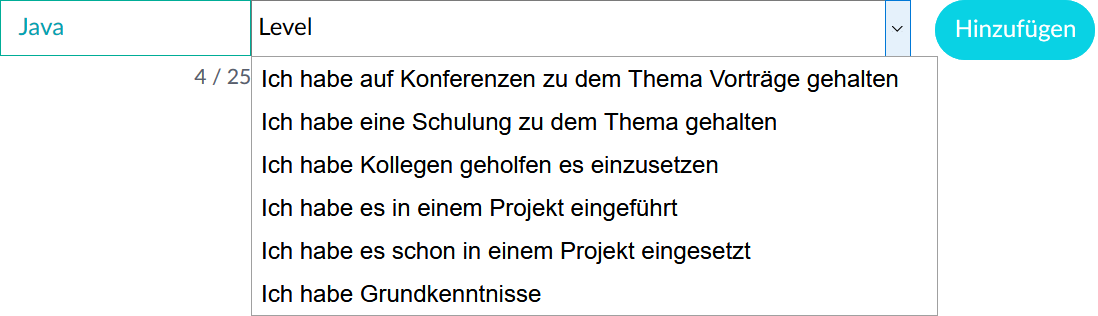
\includegraphics[width=1\textwidth]{gfx/skill-level.png}
	\caption{Hinzufügen einer Fähigkeit mit Angabe des entsprechenden Kenntnisniveaus im EXXETA-Intranet}
	\label{fig:methodik:versuchsaufbau:daten:abb1}
\end{figure}

Die in Abbildung \ref{fig:methodik:versuchsaufbau:daten:abb1} dargestellten Abstufungen werden beim Speichern in ganzzahlige Werte von null ("Ich habe Grundkenntnisse") bis sechs ("Ich habe auf Konferenzen zu dem Thema Vorträge gehalten") übertragen.

Aufgrund dieser klaren Beschreibungen der einzelnen Stufen in Abbildung \ref{fig:methodik:versuchsaufbau:daten:abb1} kann Bias bei der Selbsteinschätzung weitgehend ausgeschlossen werden. Außerdem ist es in der vorliegenden Problemstellung gut möglich, dass einzelne Mitarbeiter ihre Kompetenzen grundsätzlich besser oder schlechter einschätzen als andere Kollegen. Dieser Sachverhalt kann insbesondere auf längere Berufserfahrung zurückgeführt werden. Daher wird bei der Empfehlungsbestimmung auf eine Mittelwert-Zentrierung verzichtet.

Die Kompetenzen der Mitarbeiter und die zugehörigen Bewertungen dienen im Experiment als Eingabe für das unilaterale Empfehlungssystem.

\subsection{Unilaterales Empfehlungssystem}
\label{ch:methodik:versuchsaufbau:unilateral}
Um im unilateralen Empfehlungssystem Mitarbeiter für offene Projektpositionen vorzuschlagen, wird die Katz-Zentralität angewendet. Dieser speicherbasierte Graphenalgorithmus wurde in Kapitel \ref{ch:empfehlungssysteme:cf:speicherbasiert} vorgestellt. Ein Nutzen dieses Ansatzes ist die zuverlässige Lösung des Sparsity Problems. Vorteilhaft gegenüber modellbasierten Methoden ist außerdem die Langlebigkeit des Verfahrens. Sollten sich nach Durchführung des Experiments Daten im Unternehmen signifikant verändern oder neue Kompetenzen im Intranet hinzugefügt werden, ist der speicherbasierte Ansatz weiterhin unverändert anwendbar. Die dabei zu erwartende hohe Komplexität ist in der vorliegenden Problemstellung tolerierbar, da sich zum Zeitpunkt des Experiments unter 1.000 Mitarbeiter im Unternehmen befinden.

Um neben dem Sparsity Problem auch den Kaltstart zu beheben, werden zusätzlich zu den Fähigkeiten der Mitarbeiter auch deren Teamzuordnungen in Form eines hybriden Ansatzes beachtet. Bei der EXXETA AG arbeiten stets Mitarbeiter in einem Team, welche ähnliche Kompetenzen beherrschen. Der Leiter des Teams ist eine fachliche Führungskraft, dessen Fähigkeiten in der Regel repräsentativ für sein Team sind. Seine Kompetenzen sind jedoch stärker ausgeprägt. Um Rechenleistung einzusparen, werden die Teams nicht als zusätzliche Knoten in den Graphen eingefügt. Die Beziehungen werden stattdessen über direkte Kanten zwischen Kollegen dargestellt. Das Kantengewicht von Teammitglieder zu Teammitglied beträgt eins und das Gewicht von Teammitglied zu seinem Manager zwei. Über diesen Ansatz sind alle Teammitglieder schwach miteinander verbunden, sodass auch für Mitarbeiter ohne vergebene Bewertungen aussagekräftige Beurteilungen bestimmt werden können. Außerdem erhalten die Teammanager durch das höhere Kantengewicht eine stärkere Zentralität im Graphen.  Daher profitieren sämtliche Teammitglieder transitiv von den hinterlegten Fähigkeiten ihres Managers.

Die Fähigkeitsbewertungen und Teamzuordnungen können für alle Mitarbeiter der EXXETA AG über eine \acsu{REST}-Schnittstelle in Form von \acsu{JSON} aus dem Intranet abgefragt werden. Quellcode \ref{qc:methodik:versuchsaufbau:daten:qc1} zeigt beispielhaft einen Auszug aus den zurückgegebenen Daten von John Doe aus Tabelle \ref{tbl:empfehlungssysteme:arbeitsweise:tbl1}.

%\begin{minipage}{\linewidth}
	\lstinputlisting[
	language=json,
	caption=Beispiel für ein Mitarbeiter-\acsu{JSON} der \acsu{REST}-Schnittstelle des Intranets der EXXETA AG (Auszug),
	captionpos=b,
	label=qc:methodik:versuchsaufbau:daten:qc1
	]{gfx/john.json}
%\end{minipage}

In Quellcode \ref{qc:methodik:versuchsaufbau:daten:qc1} ist zu erkennen, dass eine Bewertung von eins in Tabelle \ref{tbl:empfehlungssysteme:arbeitsweise:tbl1} einer Beurteilung von null im zurückgegebenen \ac{JSON} entspricht. Damit ein Kantengewicht von null ausschließlich nicht vergebene Kompetenz-Einschätzungen symbolisiert, werden die Bewertungen vor Berechnung der Katz-Zentralität um eins erhöht.

Abbildung \ref{fig:methodik:versuchsaufbau:unilateral:abb1} zeigt die Darstellung der Kompetenzen und Teamzuordnungen der Mitarbeiter aus Tabelle \ref{tbl:empfehlungssysteme:arbeitsweise:tbl1} in der Form eines bipartiten Graphen. In der Grafik wird Jane Doe als Teammanager betrachtet.

\begin{figure}[h]
	\centering	
	\begin{tikzpicture}[node distance={32mm}, thick, main/.style = {draw, circle}] 
		\node[main, fill=itemcolor] (MongoDB) {$MongoDB$}; 
		\node[main, fill=itemcolor] (Python) [below right of=MongoDB] {$Python$}; 
		\node[main, fill=itemcolor] (MySQL) [above right of=Python] {$MySQL$}; 
		\node[main, fill=itemcolor] (Java) [below right of=MySQL] {$Java$}; 
		\node[main, fill=itemcolor] (HDFS) [above right of=Java] {$HDFS$}; 
		\node[main, fill=itemcolor] (Spark) [below right of=HDFS] {$Spark$};
		
		\node[main, fill=usercolor] (Jane) [above right of=MongoDB] {$Jane D.$}; 
		\node[main, fill=usercolor] (John) [above left of=HDFS] {$John D.$}; 
		\node[main, fill=usercolor] (Max) [below of=MySQL] {$Max M.$};
		\node[main, fill=usercolor] (Erika) [above right of=HDFS] {$Erika M.$}; 
		
		\draw (Jane) -- node[midway, right] {4} (Python);
		\draw (Jane) -- node[midway, above] {3} (MySQL);
		\draw (Jane) -- node[midway, above] {3} (MongoDB);
		
		\draw (John) -- node[midway, right] {1} (HDFS);		
		\draw (John) -- node[midway, right] {3} (Java);
		\draw (John) -- node[midway, above] {2} (MySQL);
		
		\draw (Erika) -- node[midway, above] {5} (HDFS);
		\draw (Erika) -- node[midway, left] {3} (Spark);
		
		\draw (Max) -- node[midway, above] {2} (Java);
		\draw (Max) -- node[midway, above] {3} (Python);
		\draw (Max) -- node[midway, right] {1} (MySQL);
		
		\draw (Jane) -- node[midway, above] {2} (John);
		\draw (Jane) -- node[midway, left] {2} (Max);
		\path (Jane) edge[bend left=25] node[midway, above] {2} (Erika);
		
		\draw (John) -- node[midway, right] {1} (Max);
		\draw (John) -- node[midway, above] {1} (Erika);
		
		\path (Max) edge[bend right=40] node[midway, below] {1} (Erika);
	\end{tikzpicture}
	
	\caption{Graph aus Abbildung \ref{fig:empfehlungssysteme:cf:speicherbasiert:abb2} mit zusätzlicher Teamzuordnung}
	\label{fig:methodik:versuchsaufbau:unilateral:abb1}
\end{figure}

Zur Anwendung des unilateralen Empfehlungssystems gibt ein Projektmanager die für eine offene Projektposition relevanten Fähigkeiten mitsamt des benötigten Kompetenzniveaus in das System ein. Diese Daten werden wie in Kapitel \ref{ch:empfehlungssysteme:cf:speicherbasiert} im Kontext der Gruppen-Recommender Engines beschrieben, in Form eines Pseudo-Mitarbeiters ebenfalls in den bipartiten Graphen aus Abbildung \ref{fig:methodik:versuchsaufbau:unilateral:abb1} eingefügt. Anhand dieser Daten folgt die Bestimmung der Katz-Zentralität. Anschließend wird für jede vom Projektmanager geforderte Kompetenz die absolute Differenz zwischen Pseudomitarbeiter und allen anderen Angestellten bestimmt. Im letzten Schritt werden die Mitarbeiter nach geringster Abweichung sortiert und an den Projektmanager zurückgegeben.

\subsection{Bilaterales Empfehlungssystem}
\label{ch:methodik:versuchsaufbau:bilateral}

\newpage
Zu erhebende Daten:\\
- Für jeden Mitarbeiter erheben: Wichtigkeit (true/false) --> Auch für Dinge, die man noch nicht kann\\
- Für jeden Mitarbeiter erheben: Welche Auswirkung hat es, wenn im Projekt nicht ausgelastet (Kurve A bis C) --> Alle drei Antwortmöglichkeiten positiv formulieren --> z.B. Freiräume nutzen

Erstellen des Graphen:\\
- Aus Skills (kollaboratives Filtern) und Teamzuordnung (Inhaltsbasiertes Filtern) einen tripartiten Graphen erstellen\\

Eingabe der offenen Projektposition:\\
- Benötigt: Fähigkeiten und Wichtigkeit (Boolean)

Algorithmus:\\
- Berechnung der Katz-Zentralität\\
- Für jeden relevanten Mitarbeiter auf Basis von Abbildung \ref{fig:methodik:abb2} den finalen Wert bestimmen --> Hierbei je nach Wichtigkeit die Kurve stauchen --> Wenn für Projektmanger wichtig, die durchgezogene Linie doppelt so steil; Wenn für Mitarbeiter wichtig, rechte Seite doppelt so steil; Auswahl der Kurve anhand der Information des Mitarbeiters\\
- Summe für alle Fähigkeiten eines Projektes für jeden Mitarbeiter berechnen

\begin{figure}[h]
	\centering
	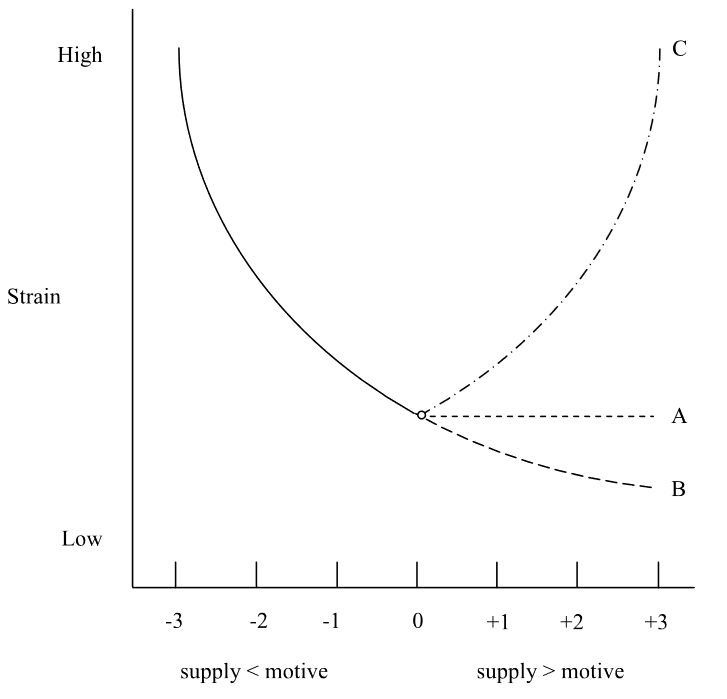
\includegraphics[width=0.75\textwidth]{gfx/ueberschuss_supply_motive.png}
	\caption{Auswirkungen eines Bedürfnisse-Angebote Misfits \cite[S. 23]{edwards:2008}\\(Bearbeitet von \myName)}
	\label{fig:methodik:abb2}
\end{figure}

- Algorithmus einmal durchführen mit Wichtigkeiten und einmal ohne (bilateral vs. unilateral)\\
- Ausgabe der sortierten Liste (mit allen Mitarbeitern (zB 25))\\
- Eingabe der Projektposition und Algorithmus für jede Projektposition wiederholen

\section{Geplante Evaluation}
\label{ch:methodik:evaluation}
Evaluation für Projektmanager:\\
- Erhält für jedes Projekt beide Listen und gibt auf einer Skala von 1 bis 5 an, wie hoch der die Leistung der empfohlenen Mitarbeiter in diesem Projekt einschätzen würde

Evaluation für Mitarbeiter:\\
- Jeder Mitarbeiter muss für jedes Projekt auf einer Skala von 1 bis 5 bewerten, wie zufrieden er wäre, wenn er darin arbeiten würde\\
- Ergebnisliste wird in Intervalle geteilt --> z.B. Zufriedenheit 5 bedeutet bei 25 Teilnehmern, dass der Nutzer im ersten Intervall sein muss --> Abweichung bestimmen --> Je weniger Abweichung, desto besser --> Durchschnittliche Abweichung von unilateral und bilateral vergleichen

Frage:\\
- Sollte Manager überhaupt Wichtigkeiten angeben?\\
	- Fähigkeiten sind Angebote und Wichtigkeiten Nachfrage\\
- Ist das Vergleichs-Vorgehen unilateral?\\
- Welche Daten müssen in den Anhang der Thesis?
\shorthandon{"}

%\shorthandoff{"}
\chapter{Forschungsergebnisse}
\label{ch:ergebnisse}

\section{Analyse von Fähigkeiten und Präferenzen}
\label{ch:ergebnisse:analyse}

\subsection{Fähigkeiten der Mitarbeiter aus dem Intranet}
\label{ch:ergebnisse:analyse:faehigkeiten}
An der Umfrage unter den Projektmitarbeitern haben N=23 Personen aus dem Fachbereich \acl{JES} der EXXETA AG teilgenommen. Diese Angestellten haben insgesamt 643 Kompetenzbewertungen im Intranet des Unternehmens abgegeben. Dies entspricht ca. 28 vergebenen Beurteilungen pro Person. Die Bewertungen verteilen sich auf 212 der \anzFaehigkeiten unterschiedlichen, im Intranet gespeicherten Fähigkeiten. Java ist mit 16 Beurteilungen die meist beherrschte Kompetenz.

Abbildung \ref{fig:ergebnisse:analyse:abb1} zeigt die im Intranet bewerteten Fähigkeiten sortiert nach Anzahl an Beurteilungen. Dabei ist der in Kapitel \ref{ch:empfehlungssysteme:cf:speicherbasiert} vorgestellte lange (Ratten-)Schwanz gut erkennbar. Dieser ist jedoch weniger stark ausgeprägt, als in der Referenzdarstellung aus Abbildung \ref{fig:empfehlungssysteme:cf:speicherbasiert:abb1}.

\begin{figure}[h]
	\centering
	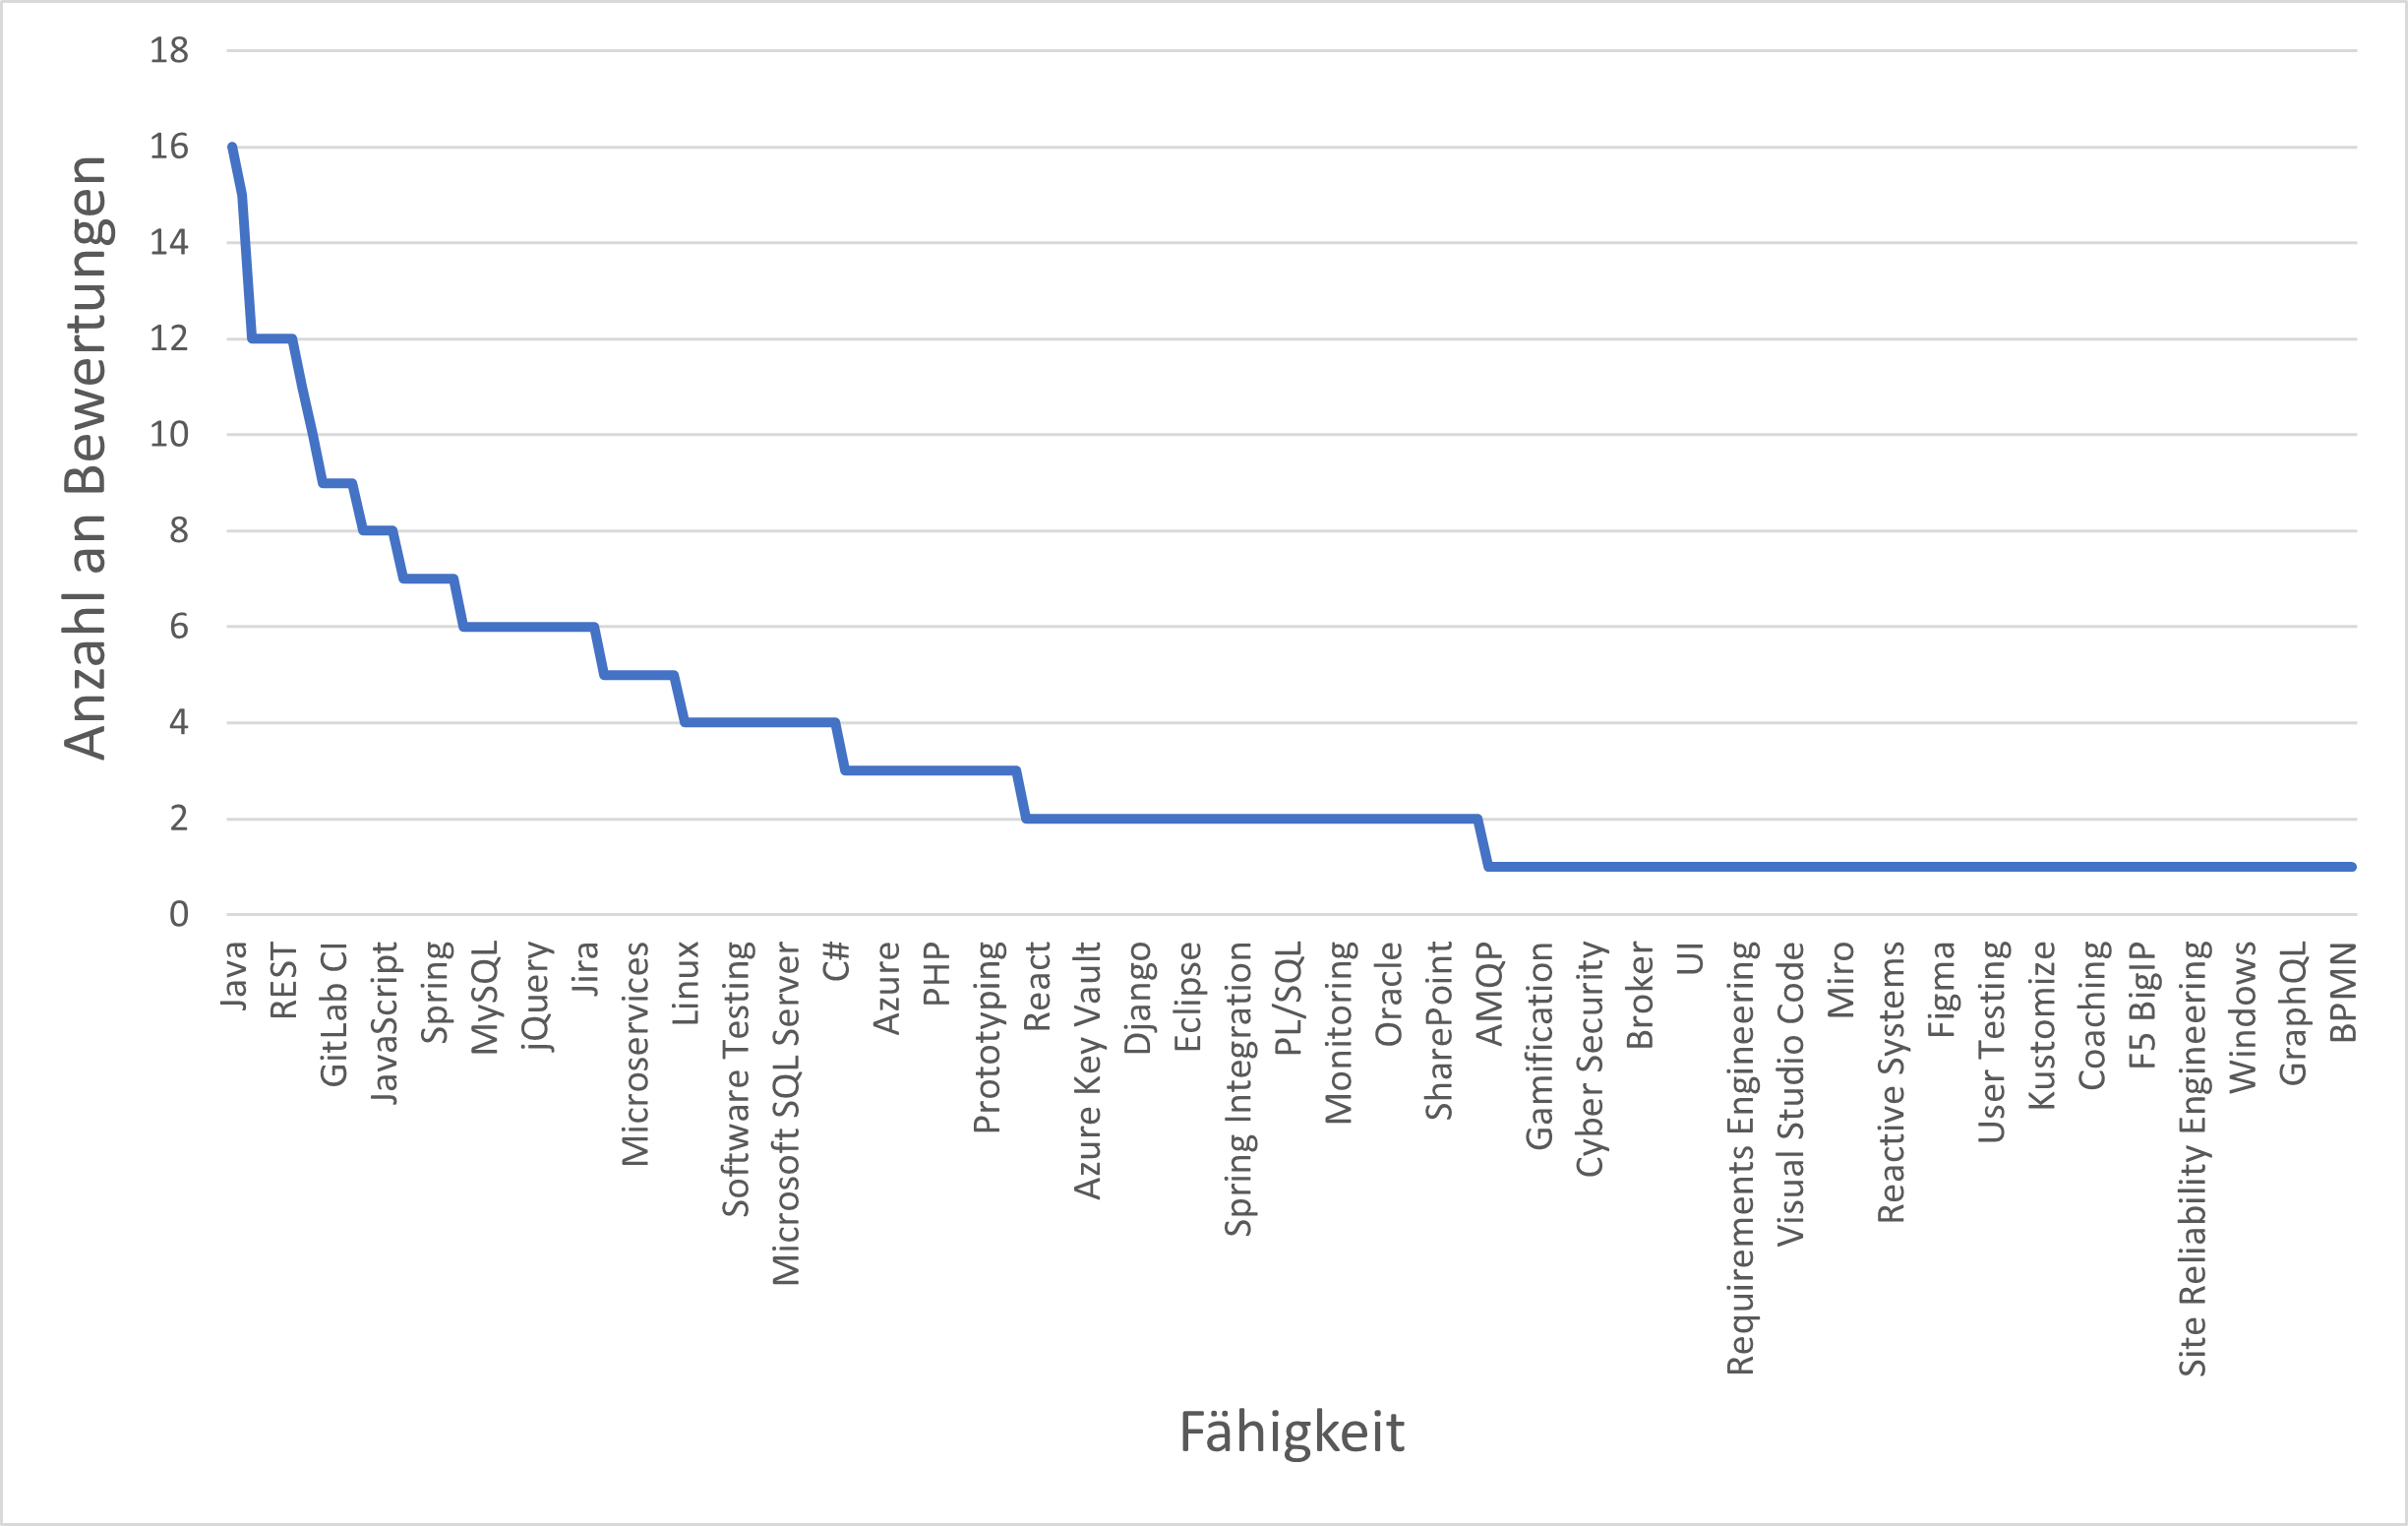
\includegraphics[width=1\textwidth]{gfx/long-tail-intranet.png}
	\caption{Langer (Ratten-)Schwanz bei den Fähigkeitsbewertungen im EXXETA-Intranet}
	\label{fig:ergebnisse:analyse:abb1}
\end{figure}

In Abbildung \ref{fig:ergebnisse:analyse:abb1} ist bezüglich des langen (Ratten-)Schwanzes festzustellen, dass neun bzw. etwa 4.3 Prozent aller Fähigkeiten über zehn oder mehr Bewertungen verfügen. Dagegen haben 151 bzw. etwa 71.2 Prozent aller Kompetenzen drei oder weniger Beurteilungen.

In den vorliegenden Daten des Intranets ist darüber hinaus zu beobachten, dass vier bzw. etwa 17.4 Prozent der Mitarbeiter keine einzige Fähigkeit bewertet haben. Diese Angestellten sind seit Einführung des Kompetenz-Bewertungssystems durchgehend in einem Projekt tätig und daher von ihrer Führungskraft noch nicht zur Pflege ihrer Fähigkeiten aufgefordert worden.

\subsection{Präferenzen der Mitarbeiter aus der Umfrage}
\label{ch:ergebnisse:analyse:praeferenzen}
Bei der Umfrage zu den Präferenzen haben die Mitarbeiter insgesamt 1408 Bewertungen abgegeben, welche sich auf 370 einzelne Kompetenzen verteilen. Dies entspricht knapp über 61 abgegebenen Wünschen pro Mitarbeiter. Git ist mit 18 Beurteilungen die meist präferierte Fähigkeit. Wie in Abbildung \ref{fig:ergebnisse:analyse:abb2} zu erkennen, deutet sich auch hinsichtlich der Wünsche ein langer (Ratten-)Schwanz an, wenn die Fähigkeiten nach Anzahl an Beurteilungen sortiert dargestellt werden.
 
\begin{figure}[h]
	\centering
	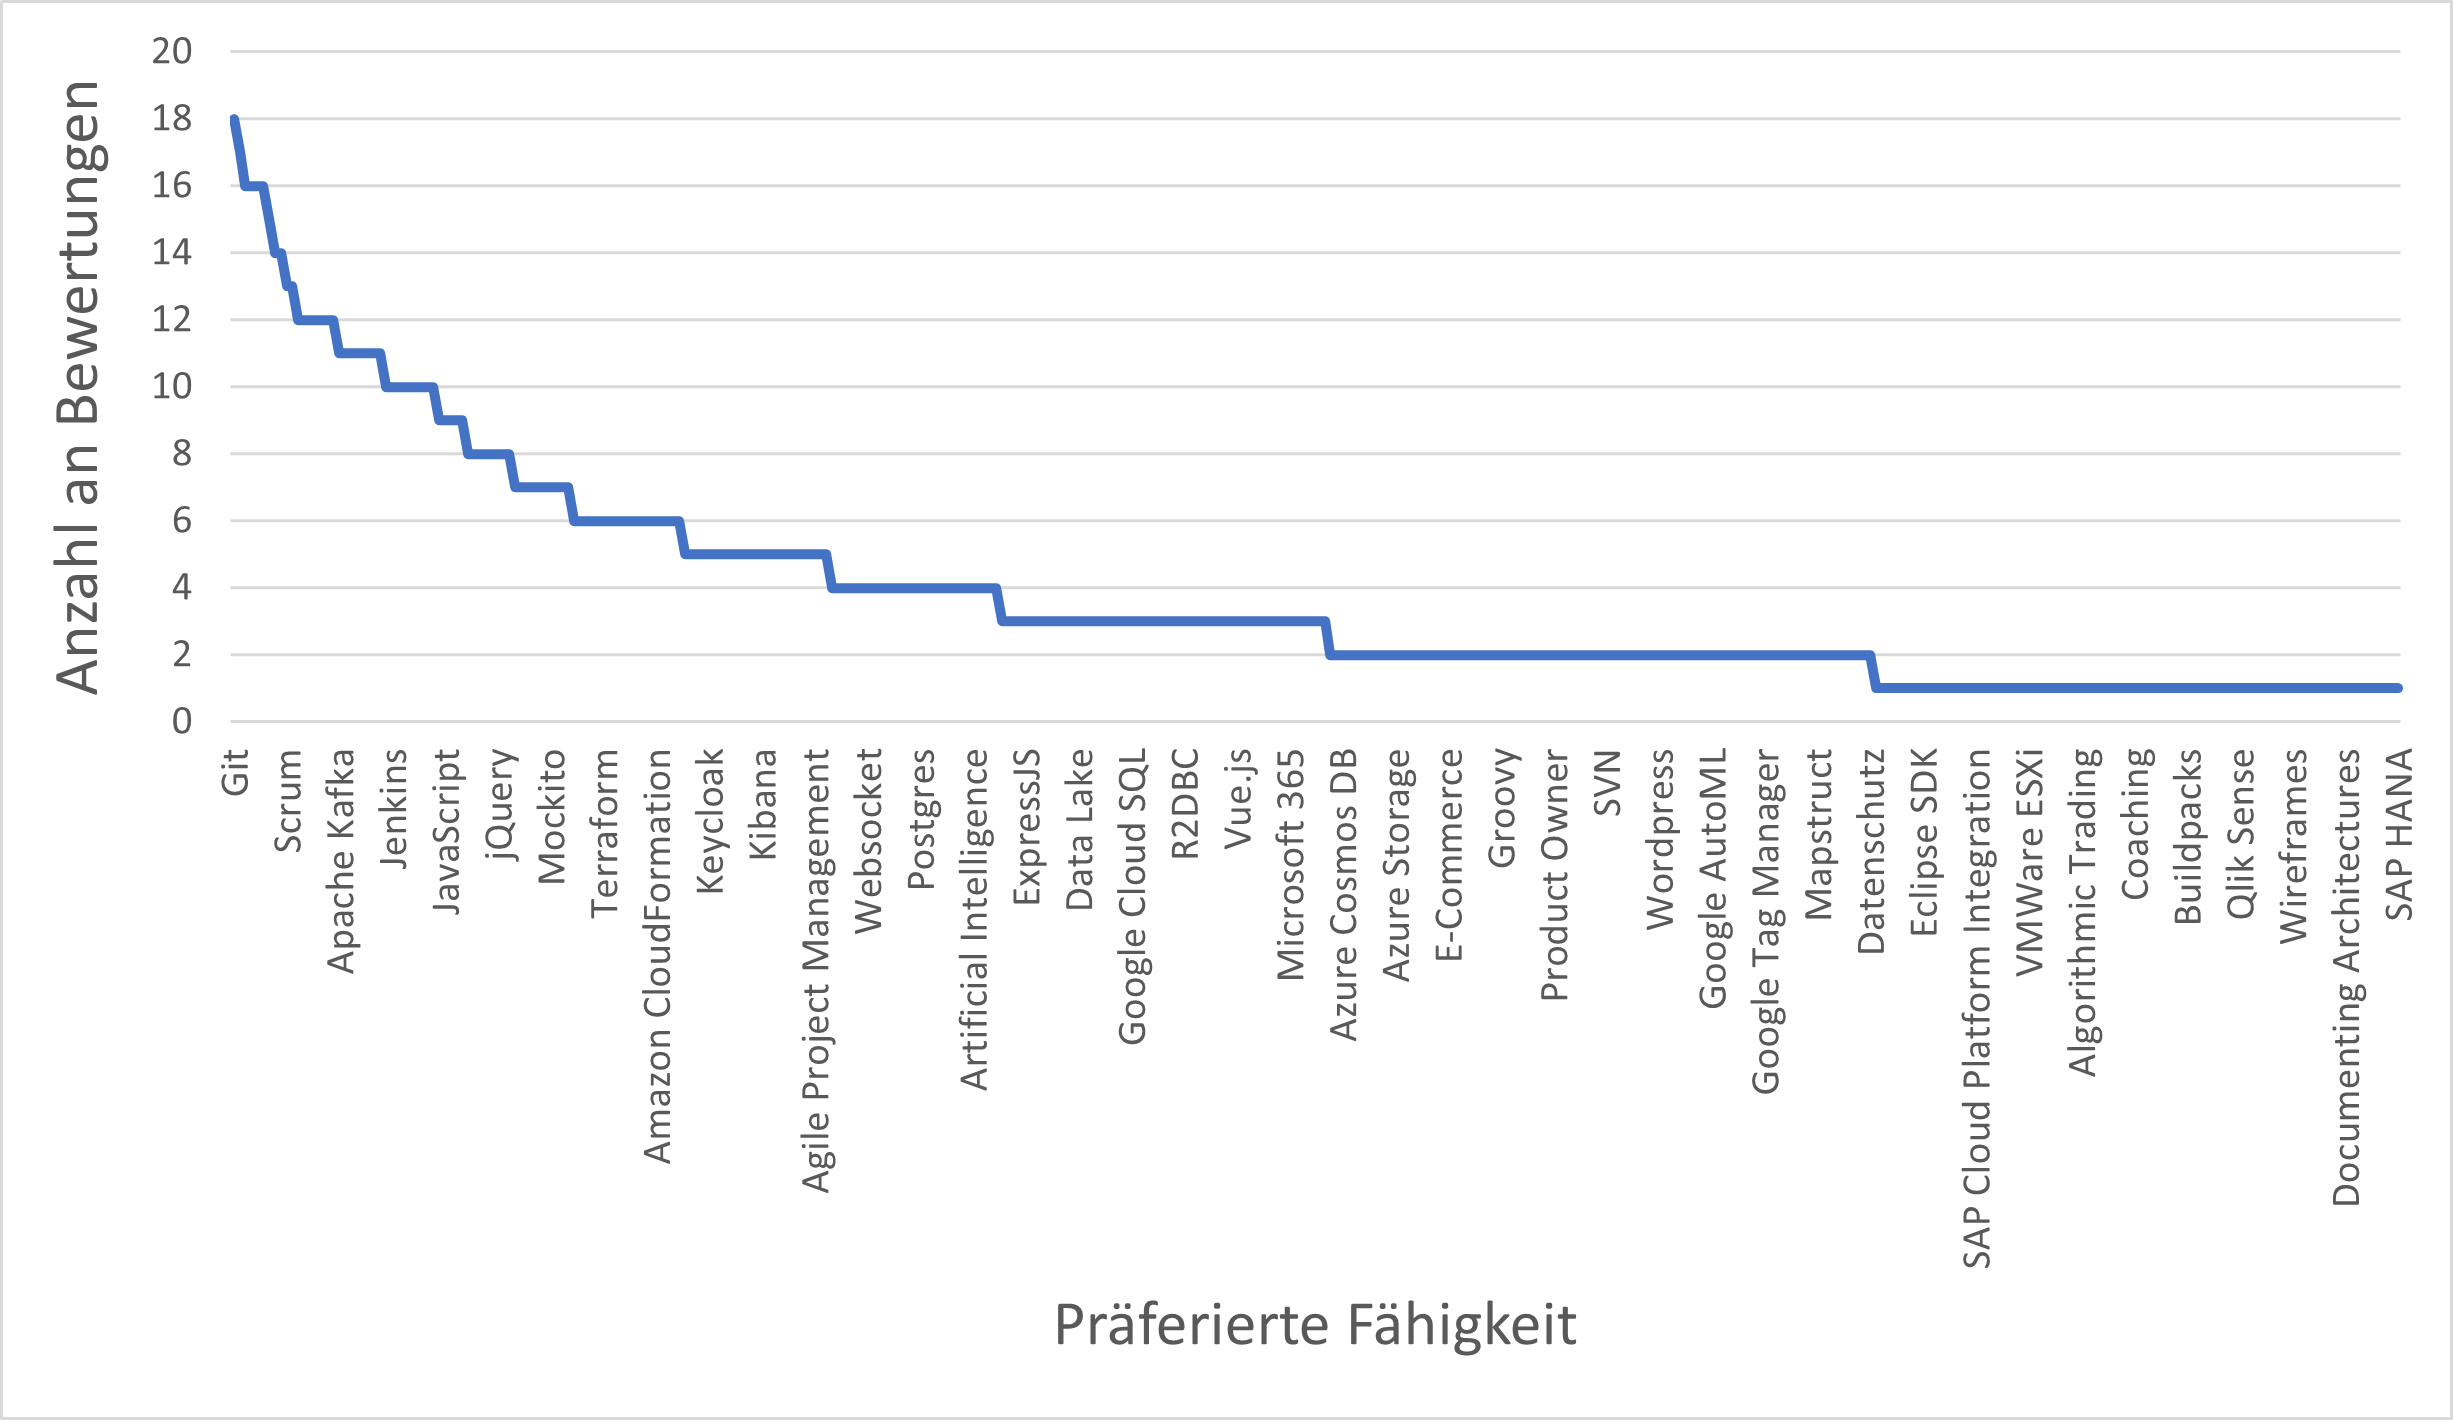
\includegraphics[width=1\textwidth]{gfx/long-tail-praeferenzen.png}
	\caption{Langer (Ratten-)Schwanz bei den präferierten Fähigkeiten der Mitarbeiter}
	\label{fig:ergebnisse:analyse:abb2}
\end{figure}

Zu Abbildung \ref{fig:ergebnisse:analyse:abb2} ist festzustellen, dass 18 bzw. etwa 4.9 Prozent aller Fähigkeiten von zwölf oder mehr Mitarbeitern präferiert werden. Dem gegenüber stehen 268 bzw. etwa 72.4 Prozent aller Kompetenzen, welche vier oder weniger Angestellte als Wunsch angegeben haben. Bei der Umfrage gab es keinen Mitarbeiter, welcher keine einzige Fähigkeit als Präferenz ausgewählte.

\subsection{Gemeinsame Betrachtung beherrschter und präferierter Fähigkeiten}
\label{ch:ergebnisse:analyse:gemeinsam}
Bei der gemeinsamen Betrachtung von Kompetenzen und Wünschen ist auf Mitarbeiterebene festzustellen, dass ein durchschnittlicher Angestellter etwa 74.7 Fähigkeiten beherrscht und/oder präferiert. Abbildung \ref{fig:ergebnisse:analyse:abb3} zeigt, wie viele dieser Kompetenzen der durchschnittliche Mitarbeiter beherrscht und wie viele er davon präferiert.

\begin{figure}[h]
	\centering
	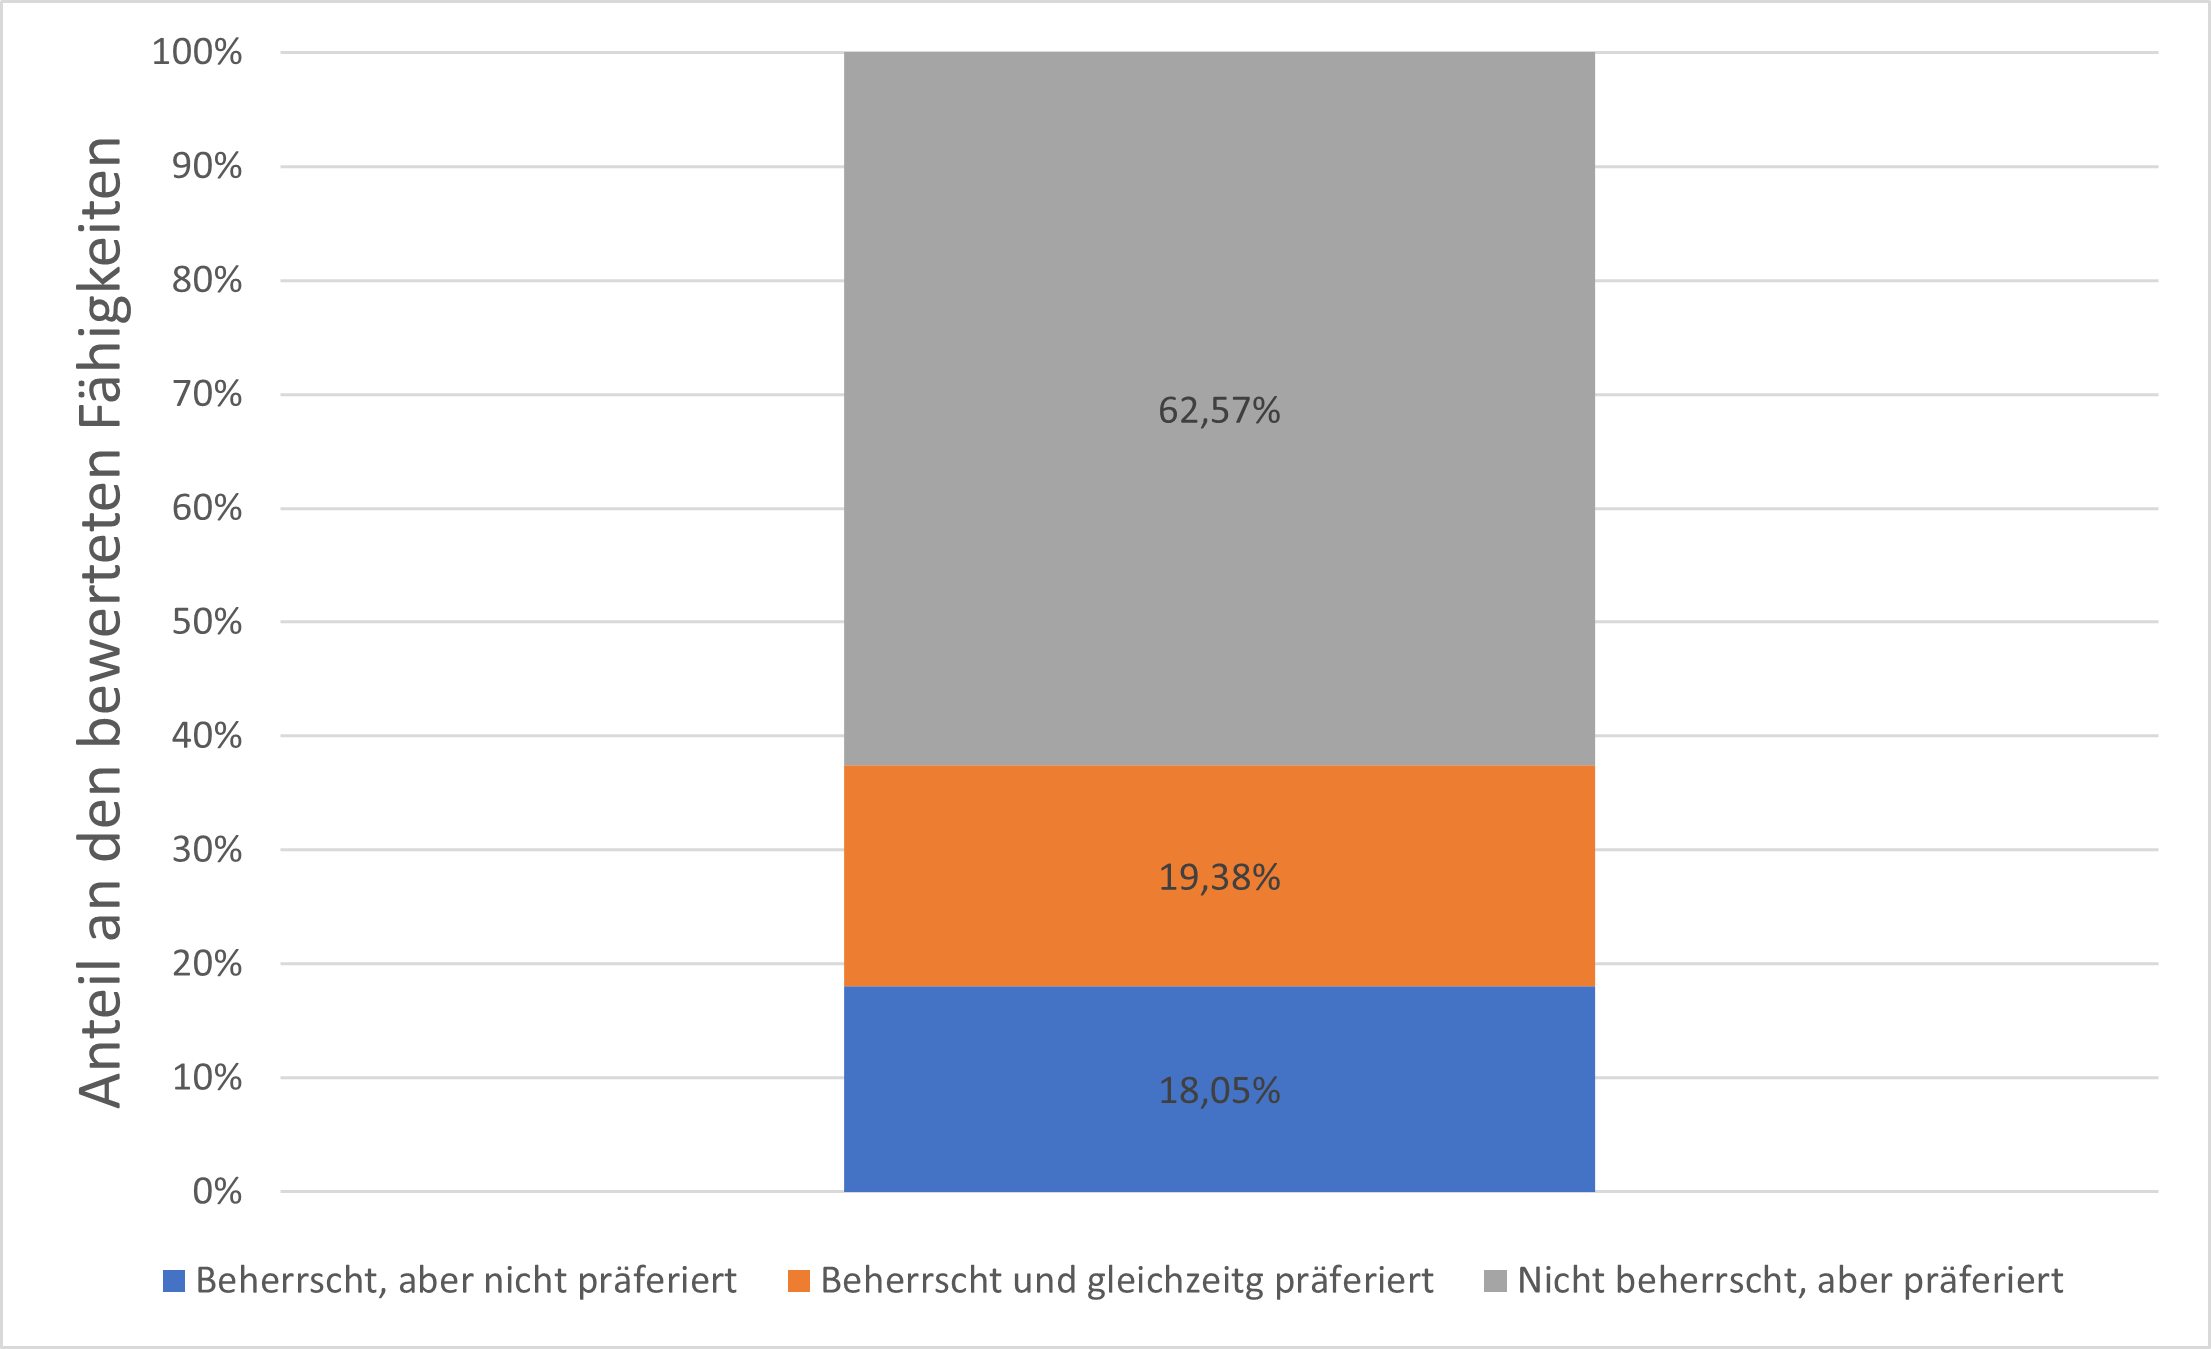
\includegraphics[width=1\textwidth]{gfx/auswertung-anteil-an-faehigkeiten.png}
	\caption{Anteil beherrschter und präferierter Fähigkeiten bei einem durchschnittlichen Mitarbeiter}
	\label{fig:ergebnisse:analyse:abb3}
\end{figure}

In Abbildung \ref{fig:ergebnisse:analyse:abb3} ist zu erkennen, dass ein durchschnittlicher Angestellter etwa 28 bzw. ca. 37.4 Prozent seiner insgesamt beurteilten Kompetenzen gleichzeitig beherrscht (orangene und blaue Farbe). Von diesen Fähigkeiten präferiert er jedoch nur ca. 14.5, also knapp über die Hälfte (orangene Farbe). Demgegenüber stehen ca. 46.7 bzw. etwa 62.6 Prozent an Fähigkeiten, welche der Angestellte zwar präferiert, aber noch nicht beherrscht (graue Farbe).

%Bei Betrachtung der beherrschten Fähigkeiten ist festzustellen, dass kaum Unterschiede zwischen präferierten und nicht gewünschten Kompetenzen ausgemacht werden können. So verfügt die durchschnittliche beherrschte, aber nicht gewünschte Fähigkeit (blaue Farbe in Abbildung \ref{fig:ergebnisse:analyse:abb3}) über eine Bewertung von 2.9 im Intranet. Die durchschnittliche vorhandene und gleichzeitig präferierte Kompetenz (orangene Farbe in Abbildung \ref{fig:ergebnisse:analyse:abb3}) verfügt über eine Bewertung von 3.1. Wie in Abbildung \ref{fig:ergebnisse:analyse:abb4} zu erkennen, sind auch bei Betrachtung der Fähigkeiten auf ihren jeweiligen Kompetenzniveaus kaum Differenzen auszumachen.
%\begin{figure}[h]
%	\centering
%	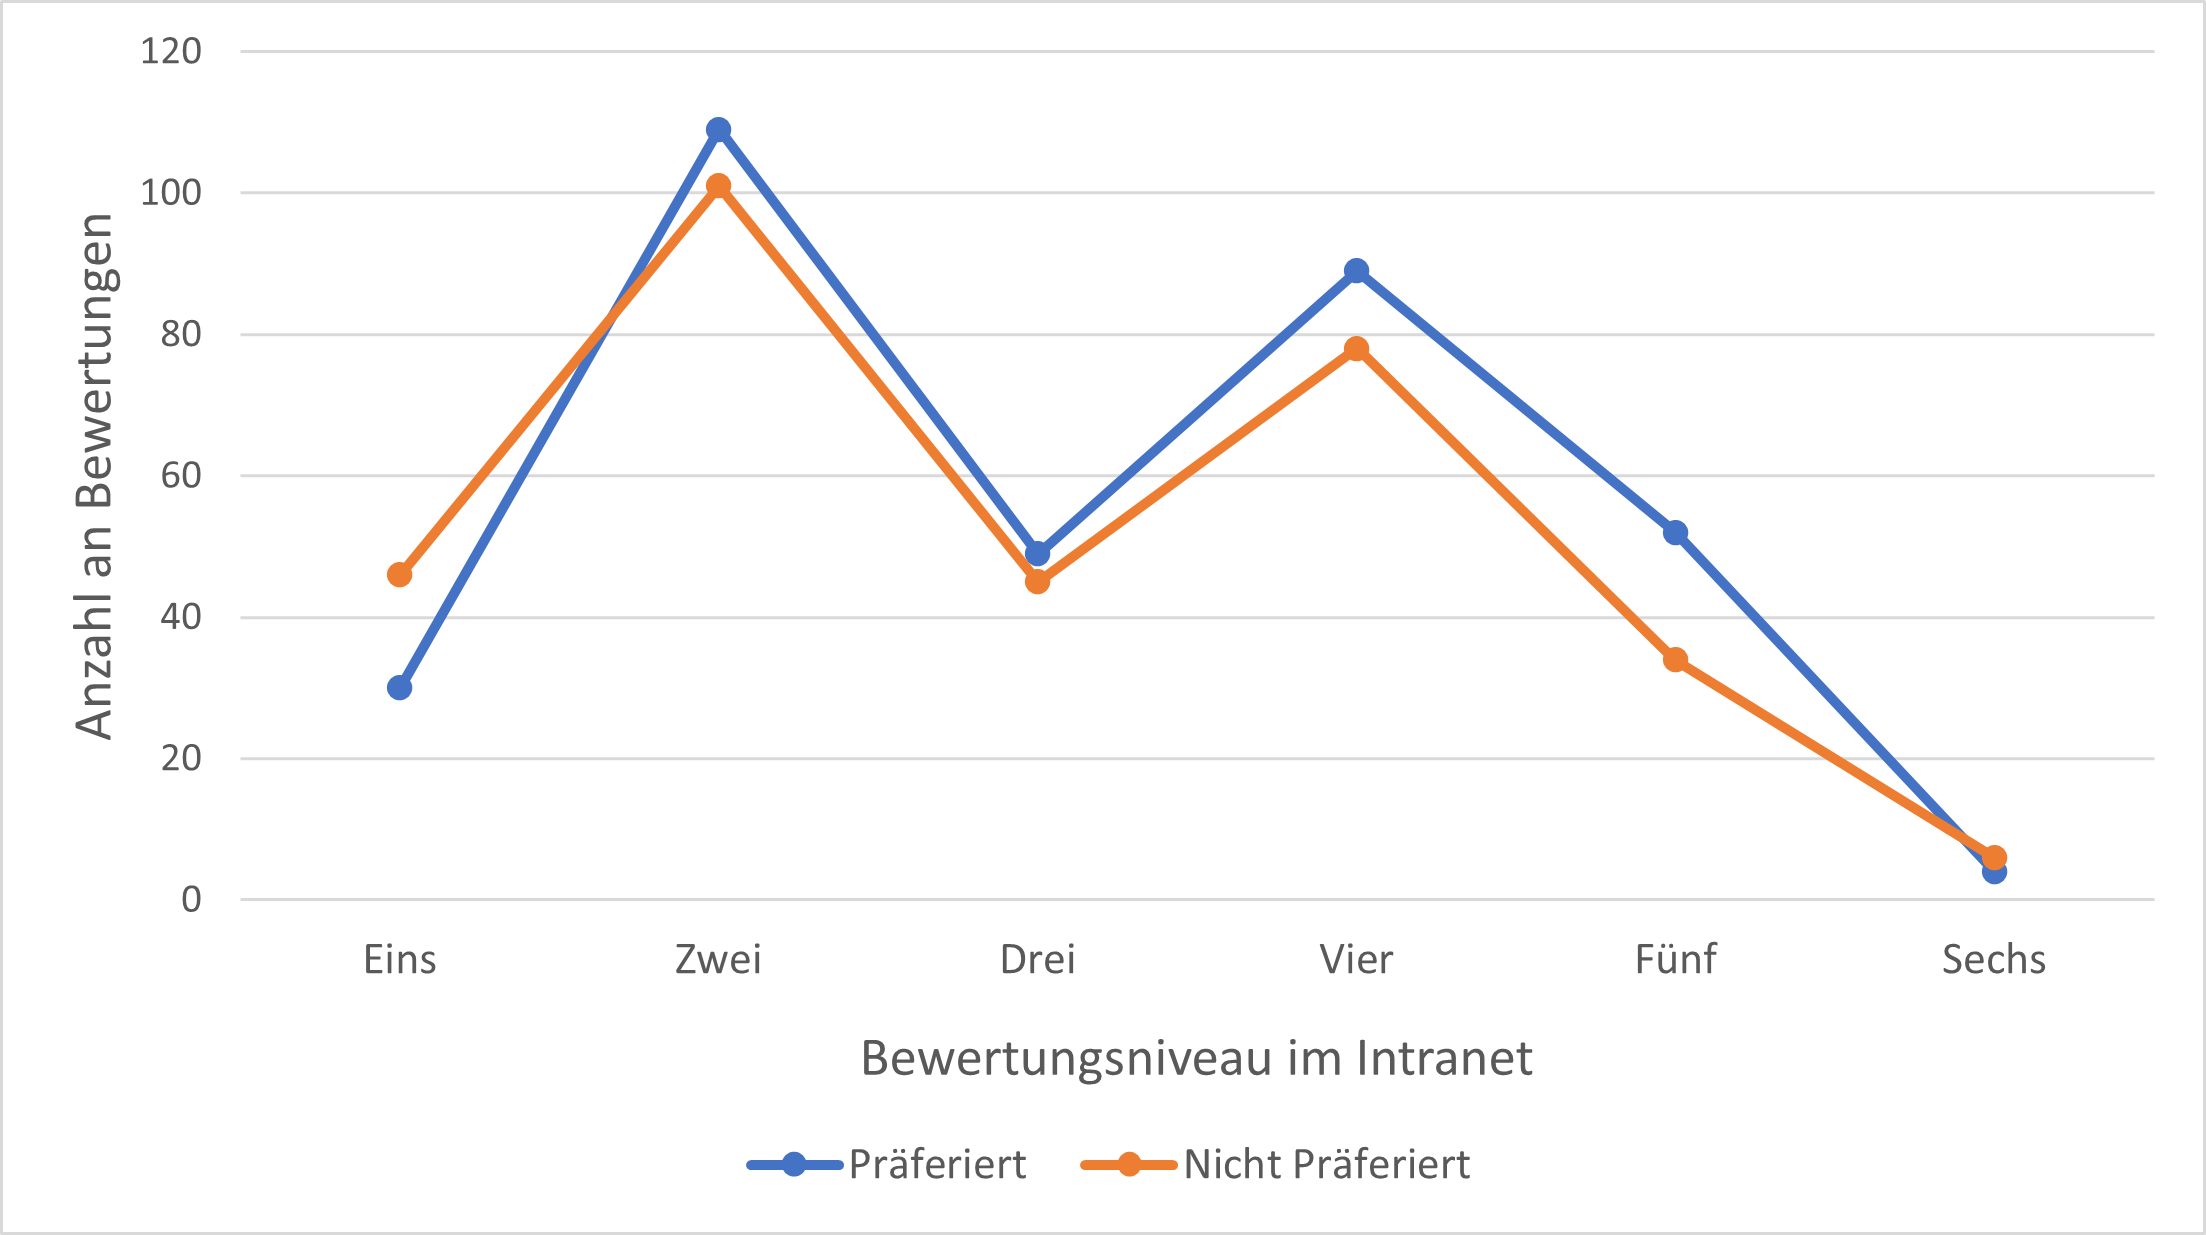
\includegraphics[width=0.8\textwidth]{gfx/bewertungen-je-bewertungsniveau.png}
%	\caption{Anzahl beherrschter und präferierter Fähigkeiten je Bewertungsniveau}
%	\label{fig:ergebnisse:analyse:abb4}
%\end{figure}
%Bei Analyse der präferierten Fähigkeiten (graue Farbe in Abbildung \ref{fig:ergebnisse:analyse:abb3}) ist zu beobachten, dass es sich bei den meist gewünschten Kompetenzen hauptsächlich um moderne Produkte aus dem Web- und Cloud-Umfeld handelt. So zählen neben Git und Java beispielsweise Kotlin, Kubernetes, Docker, Spring Boot und AWS zu den meist präferierten Fähigkeiten.

\subsection{Gesuchte und vorhandene Fähigkeiten und Präferenzen}
\label{ch:ergebnisse:umfrageMitarbeiter:projekte}
Zur Beantwortung der Forschungsfrage wurden im Rahmen der vorliegenden Master-Thesis fünf beispielhafte Projektpositionen definiert und in Kapitel \ref{ch:methodik:evaluation} vorgestellt. Abbildung \ref{fig:ergebnisse:analyse:abb5} zeigt für jede dieser Projektpositionen, wie viele der befragten Mitarbeiter im Durchschnitt die gesuchten Fähigkeiten beherrschen bzw. präferieren.

\begin{figure}[h]
	\centering
	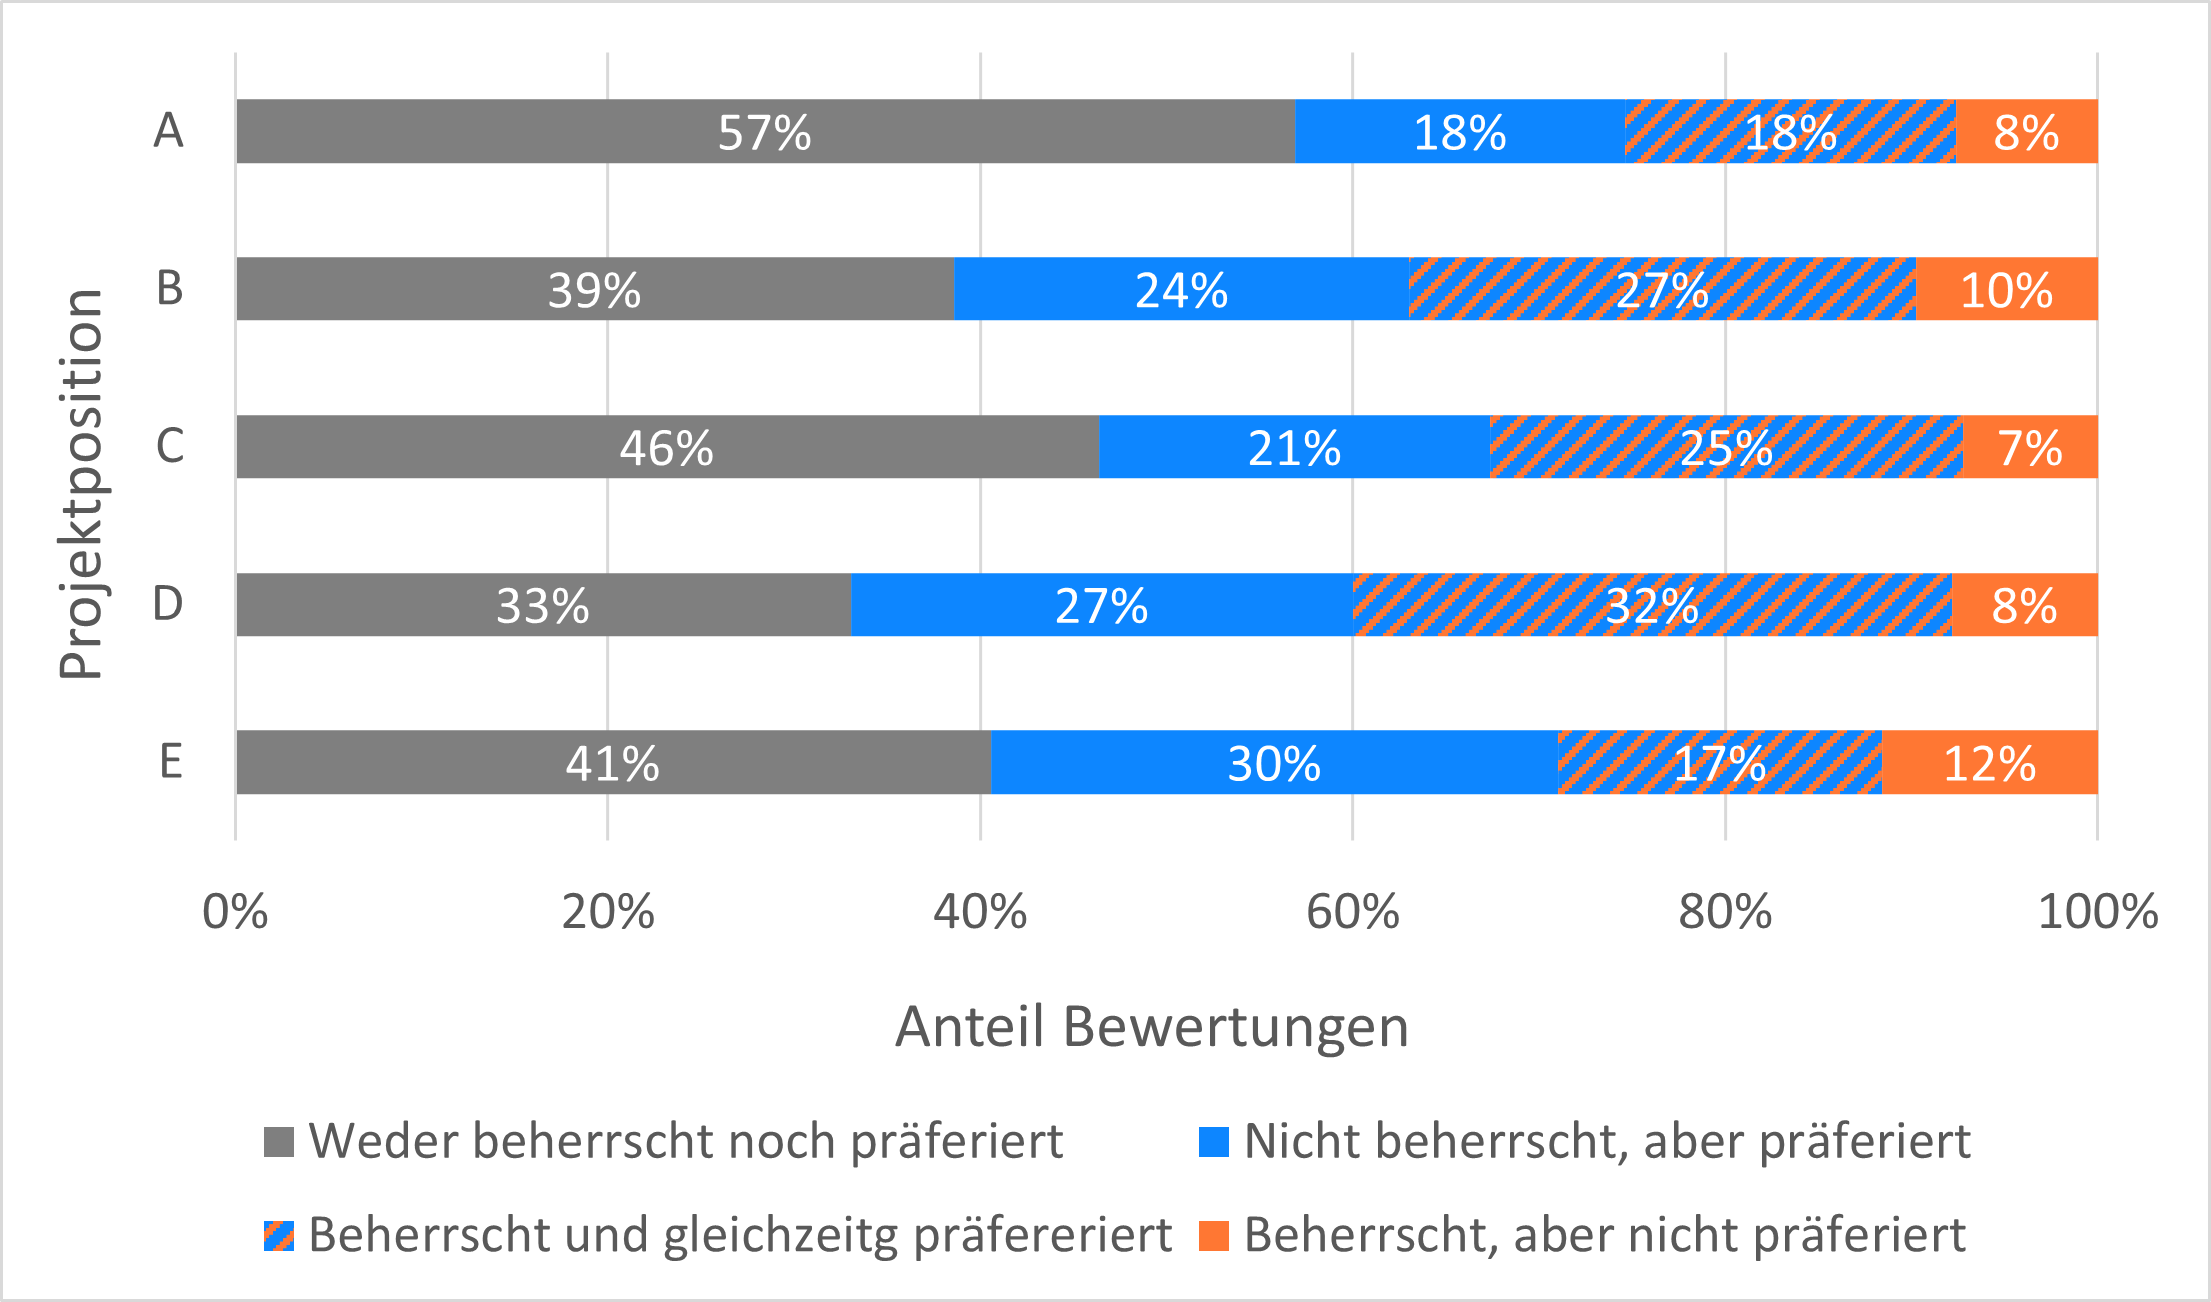
\includegraphics[width=1\textwidth]{gfx/anteil-bewertungen-je-projektposition.png}
	\caption{Anteil an Mitarbeitern, welche die in den Beispielprojektpositionen gesuchten Fähigkeiten im Durchschnitt beherrschen bzw. präferieren}
	\label{fig:ergebnisse:analyse:abb5}
\end{figure}

In Abbildung \ref{fig:ergebnisse:analyse:abb5} ist zu erkennen, dass durchschnittlich 33 Prozent aller Mitarbeiter bereits über die für die Projektpositionen benötigten Fähigkeiten verfügen. Dementsprechend beherrschen 67 Prozent aller Mitarbeiter die durchschnittlich gesuchte Kompetenz noch nicht. Es ist ebenfalls du beobachten, dass 60 Prozent aller Angestellten, welche die durchschnittlich gesuchte Kompetenz beherrschen, diese gleichzeitig präferieren. Auch ist zu erkennen, dass die Anteile an Mitarbeitern, welche die durchschnittlich gesuchte Fähigkeit beherrschen und gleichzeitig präferieren und Angestellten, welche die im Durchschnitt benötigte Kompetenz noch nicht beherrschen und dennoch präferieren mit je 24 Prozent gleich groß sind.

Bei Betrachtung jeder einzelnen in den Beispielprojektpositionen gesuchten Fähigkeit ergibt sich die Darstellung aus Abbildung \ref{fig:ergebnisse:analyse:abb6}.

\begin{figure}[h]
	\centering
	
	\subfloat[Projektposition A]{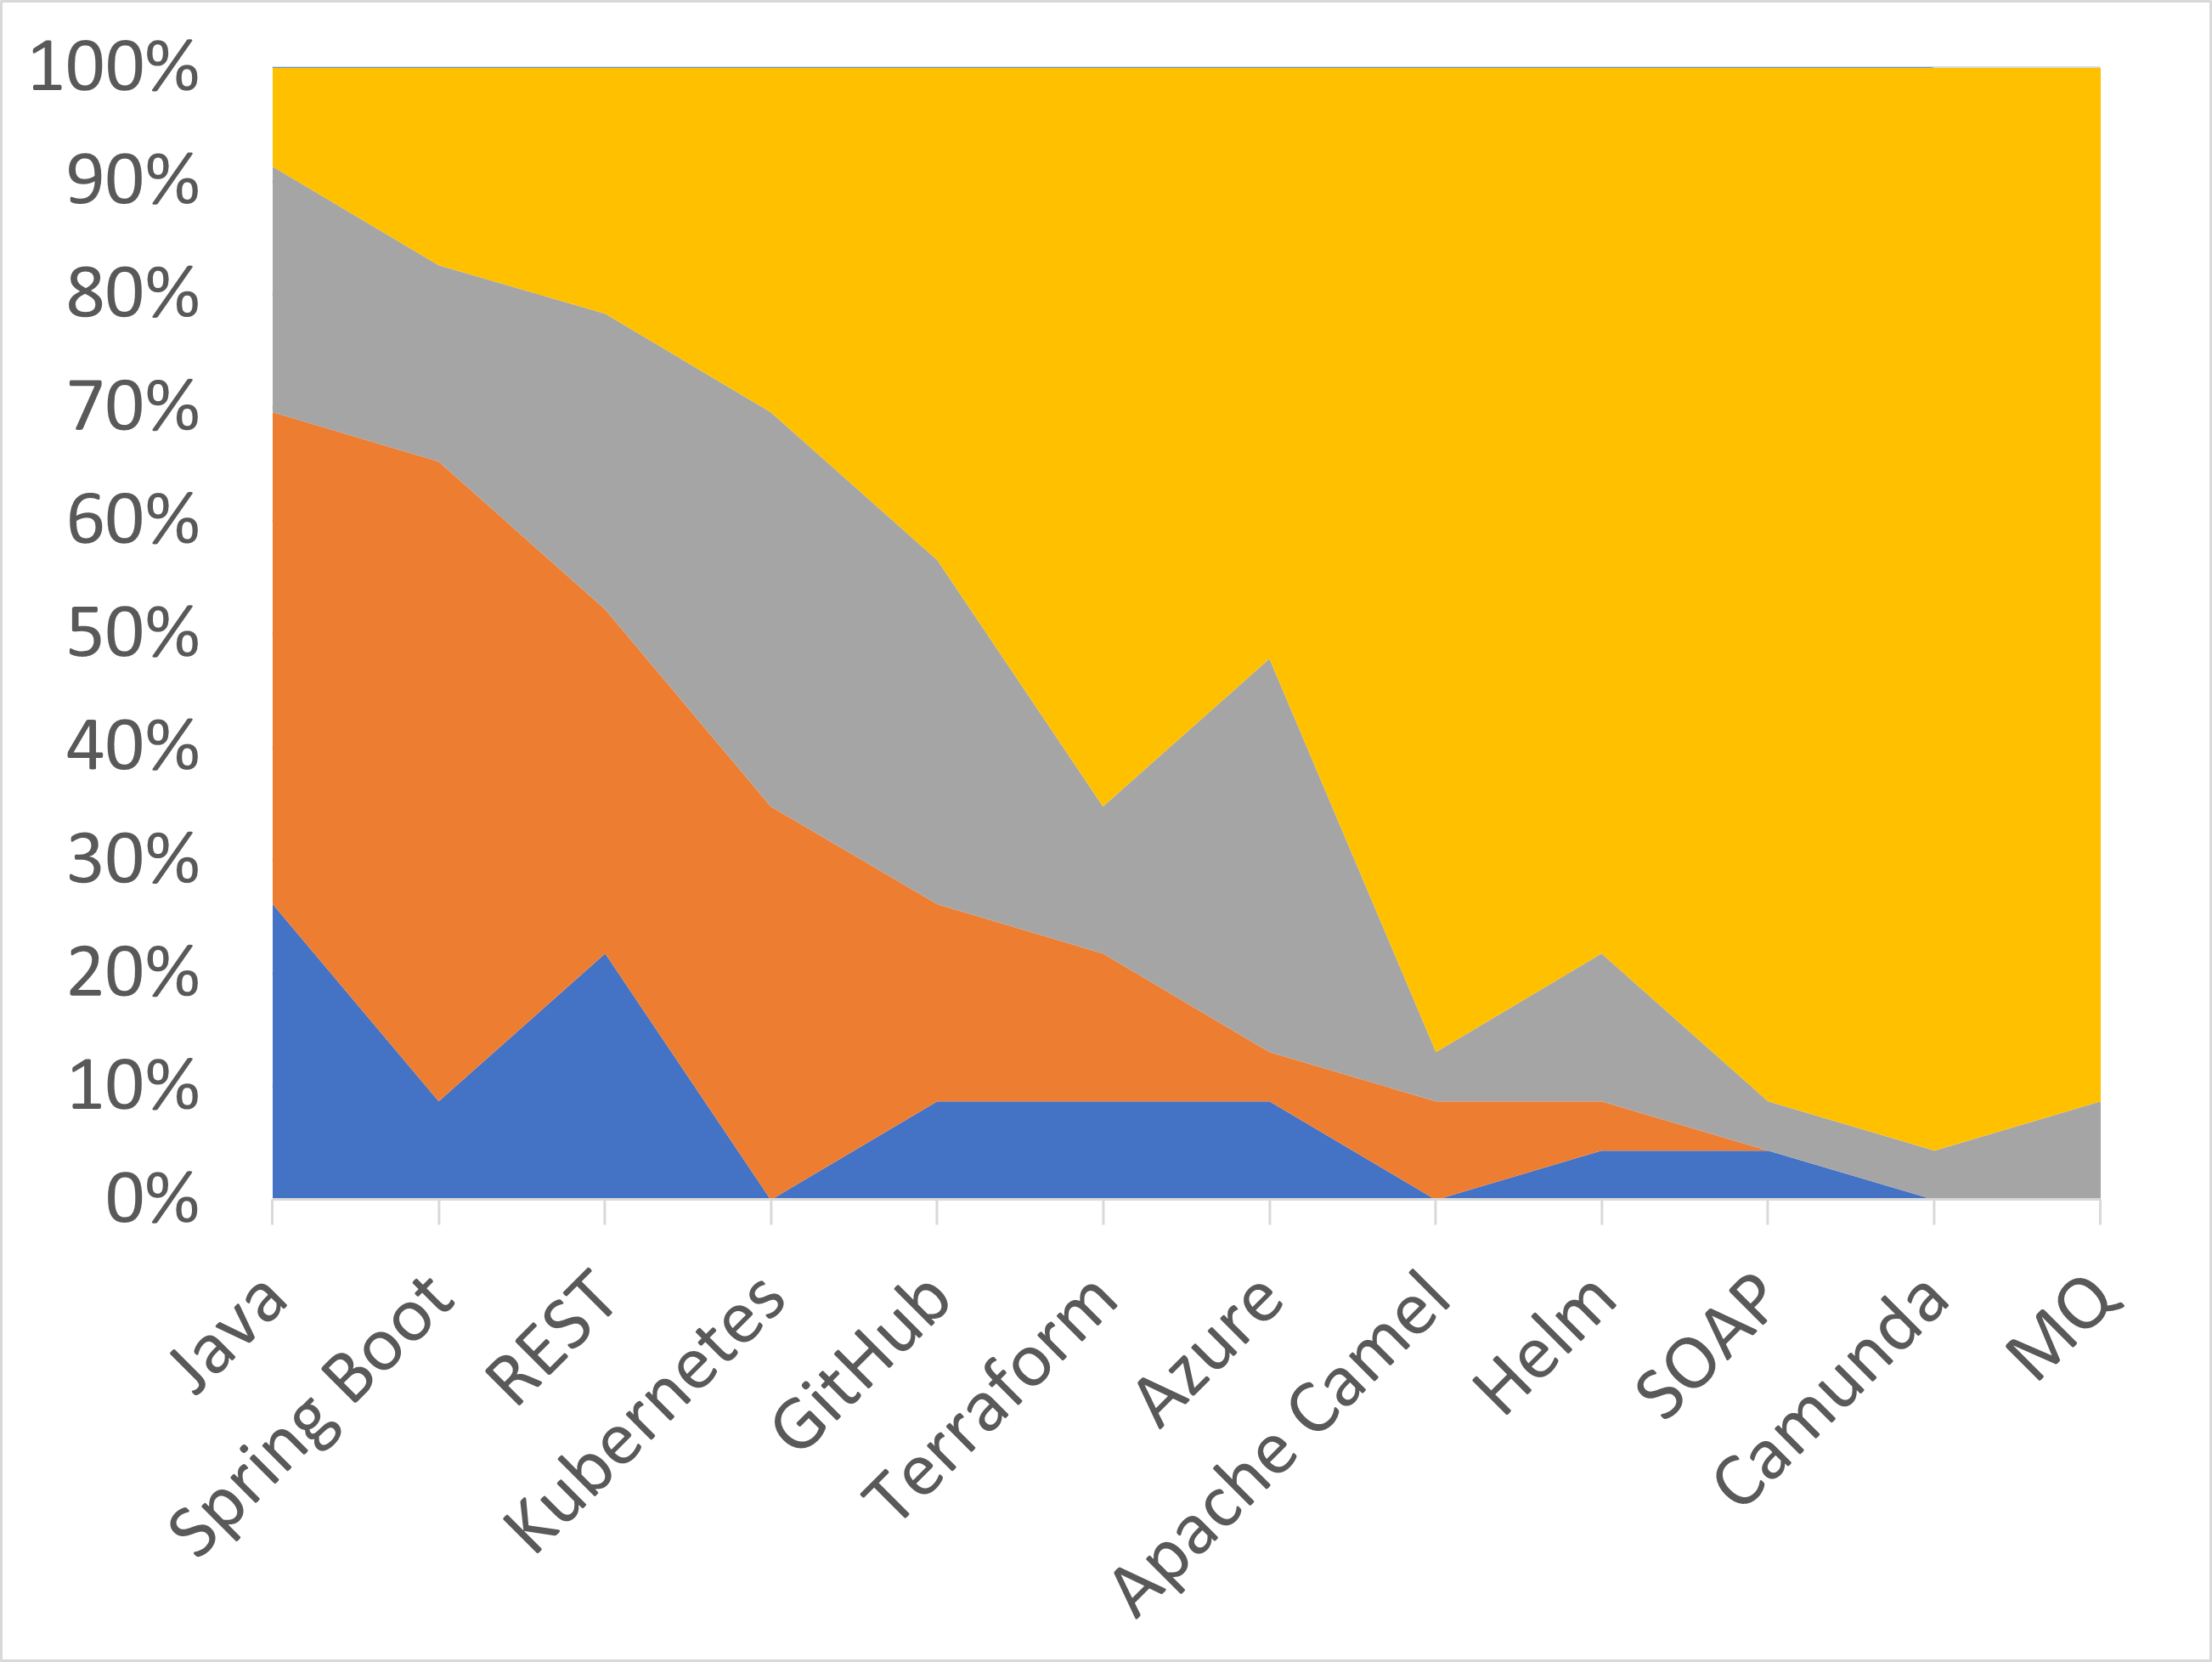
\includegraphics[width = 0.4\textwidth]{gfx/projekt-detail-a.png}}
	\subfloat[Projektposition B]{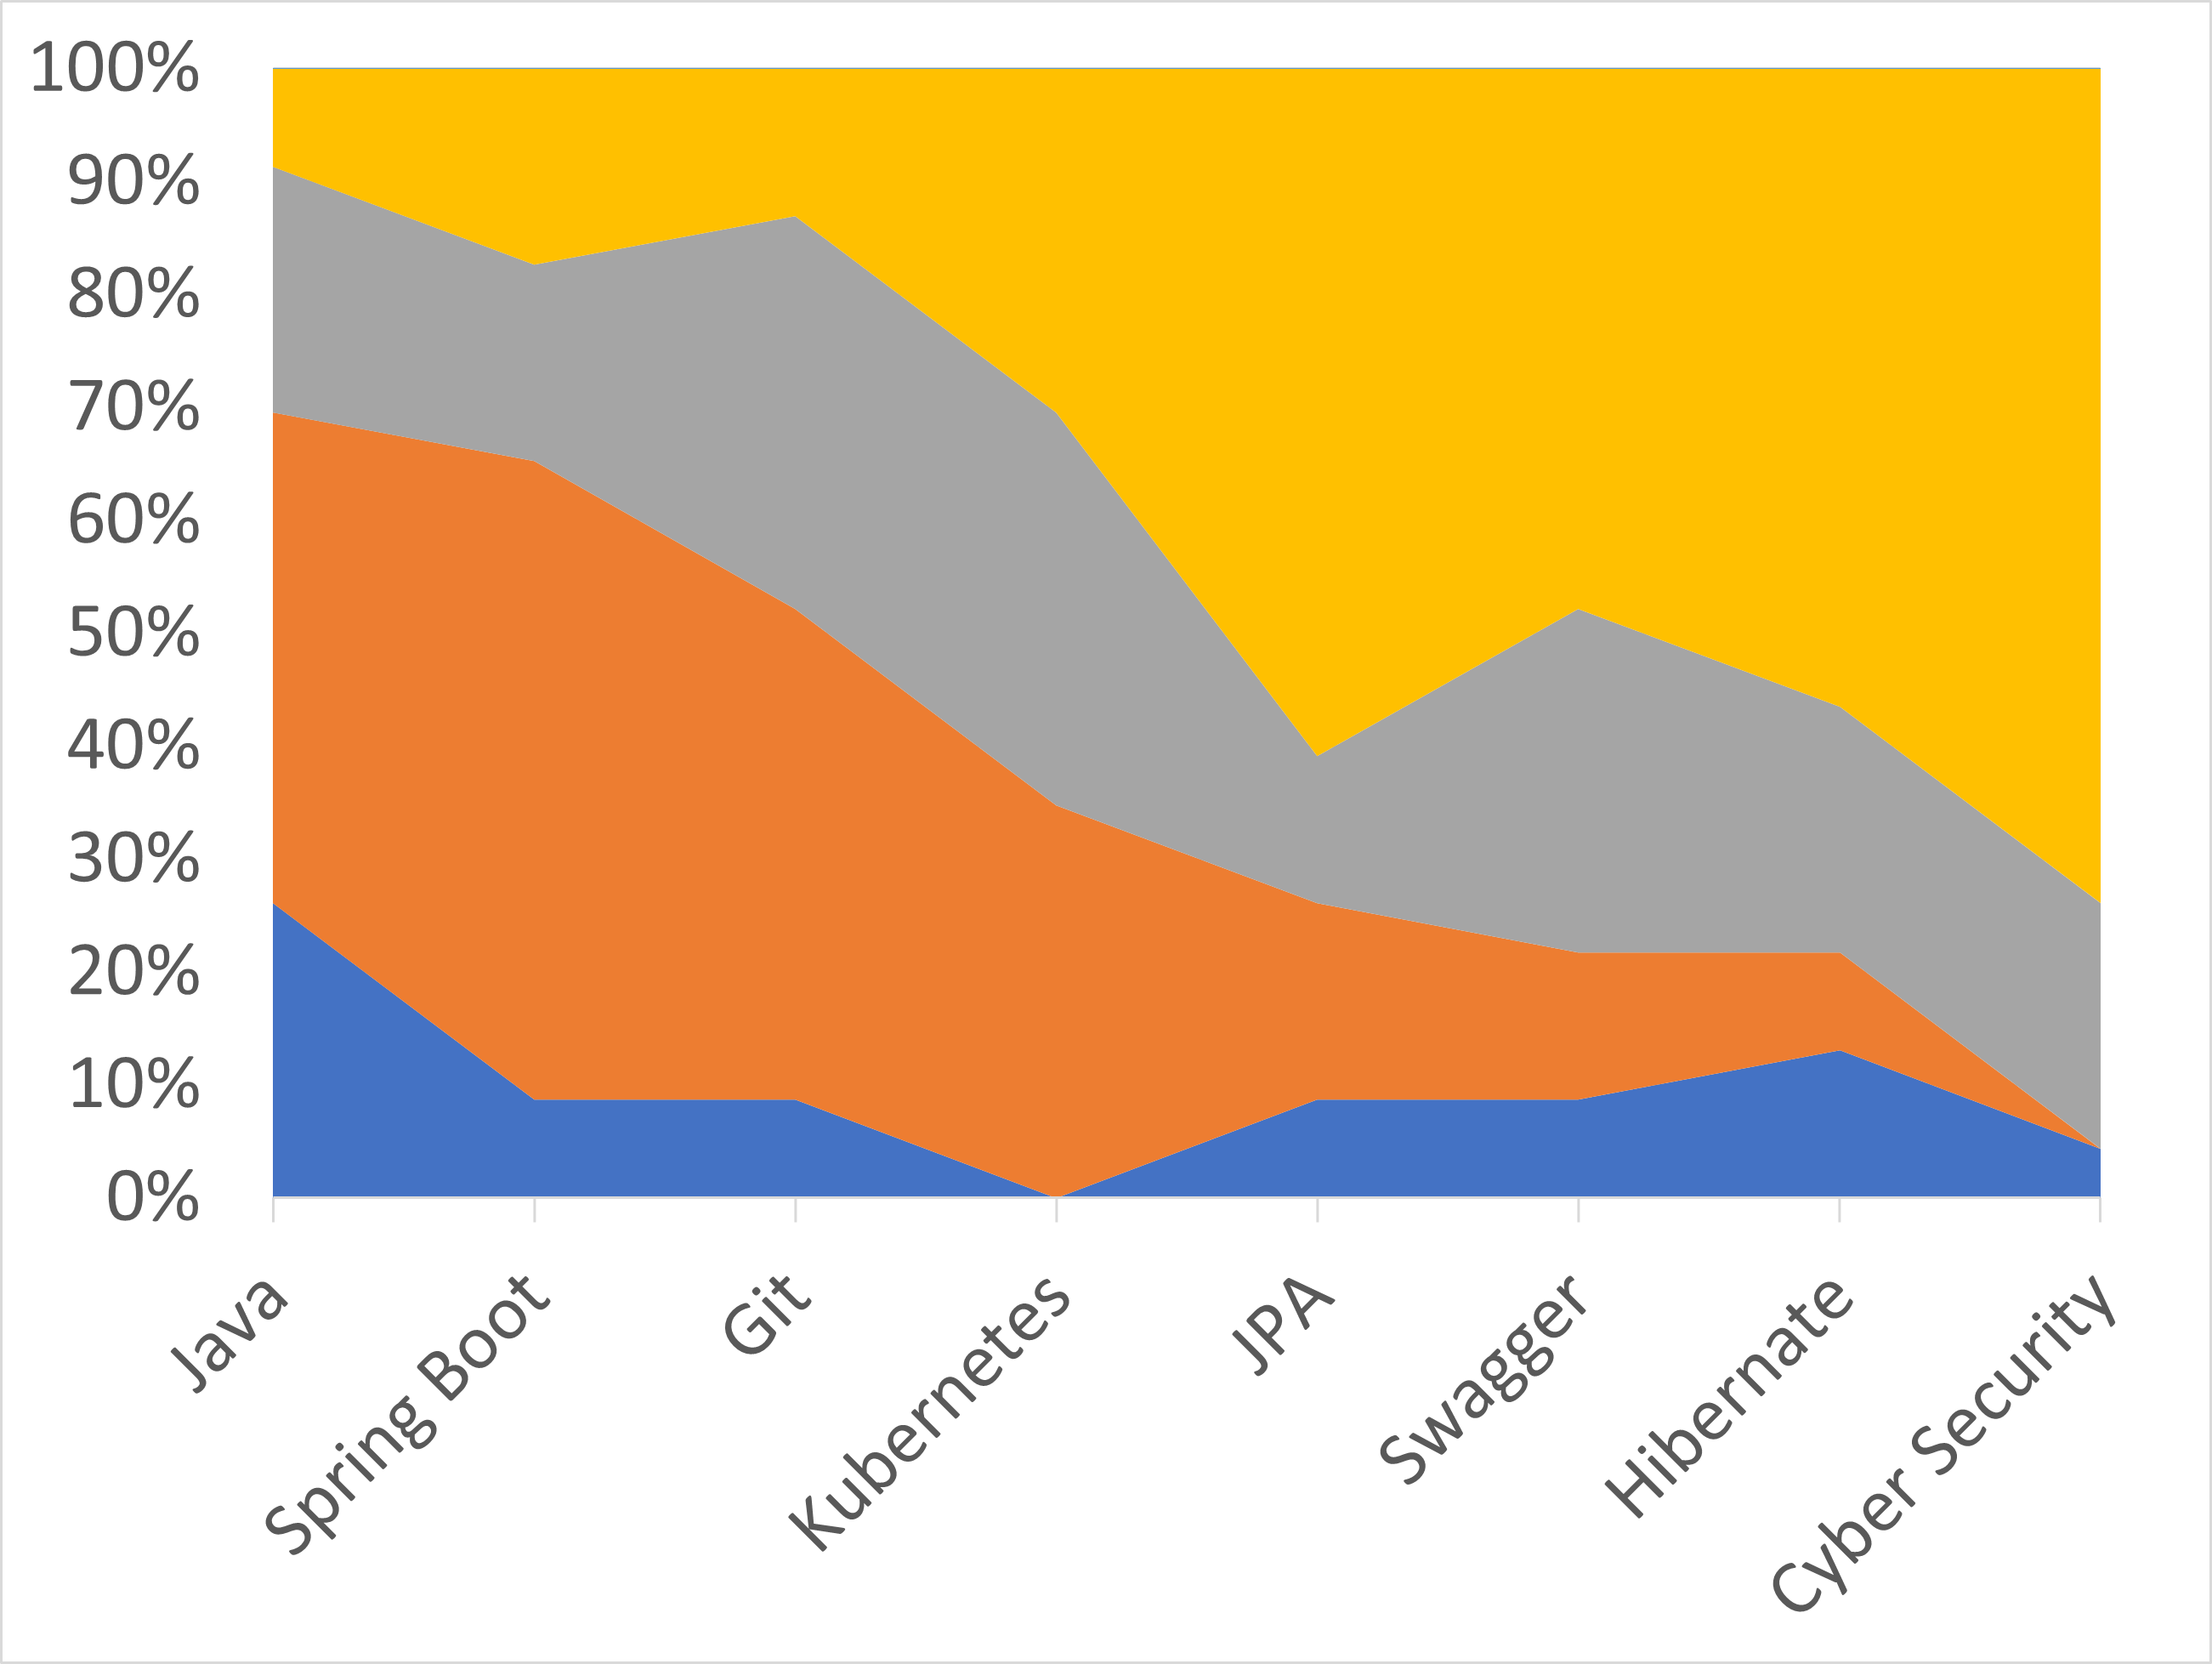
\includegraphics[width = 0.4\textwidth]{gfx/projekt-detail-b.png}}
	
\end{figure}
\begin{figure}[h]
	\centering
	\ContinuedFloat
	
	\subfloat[Projektposition C]{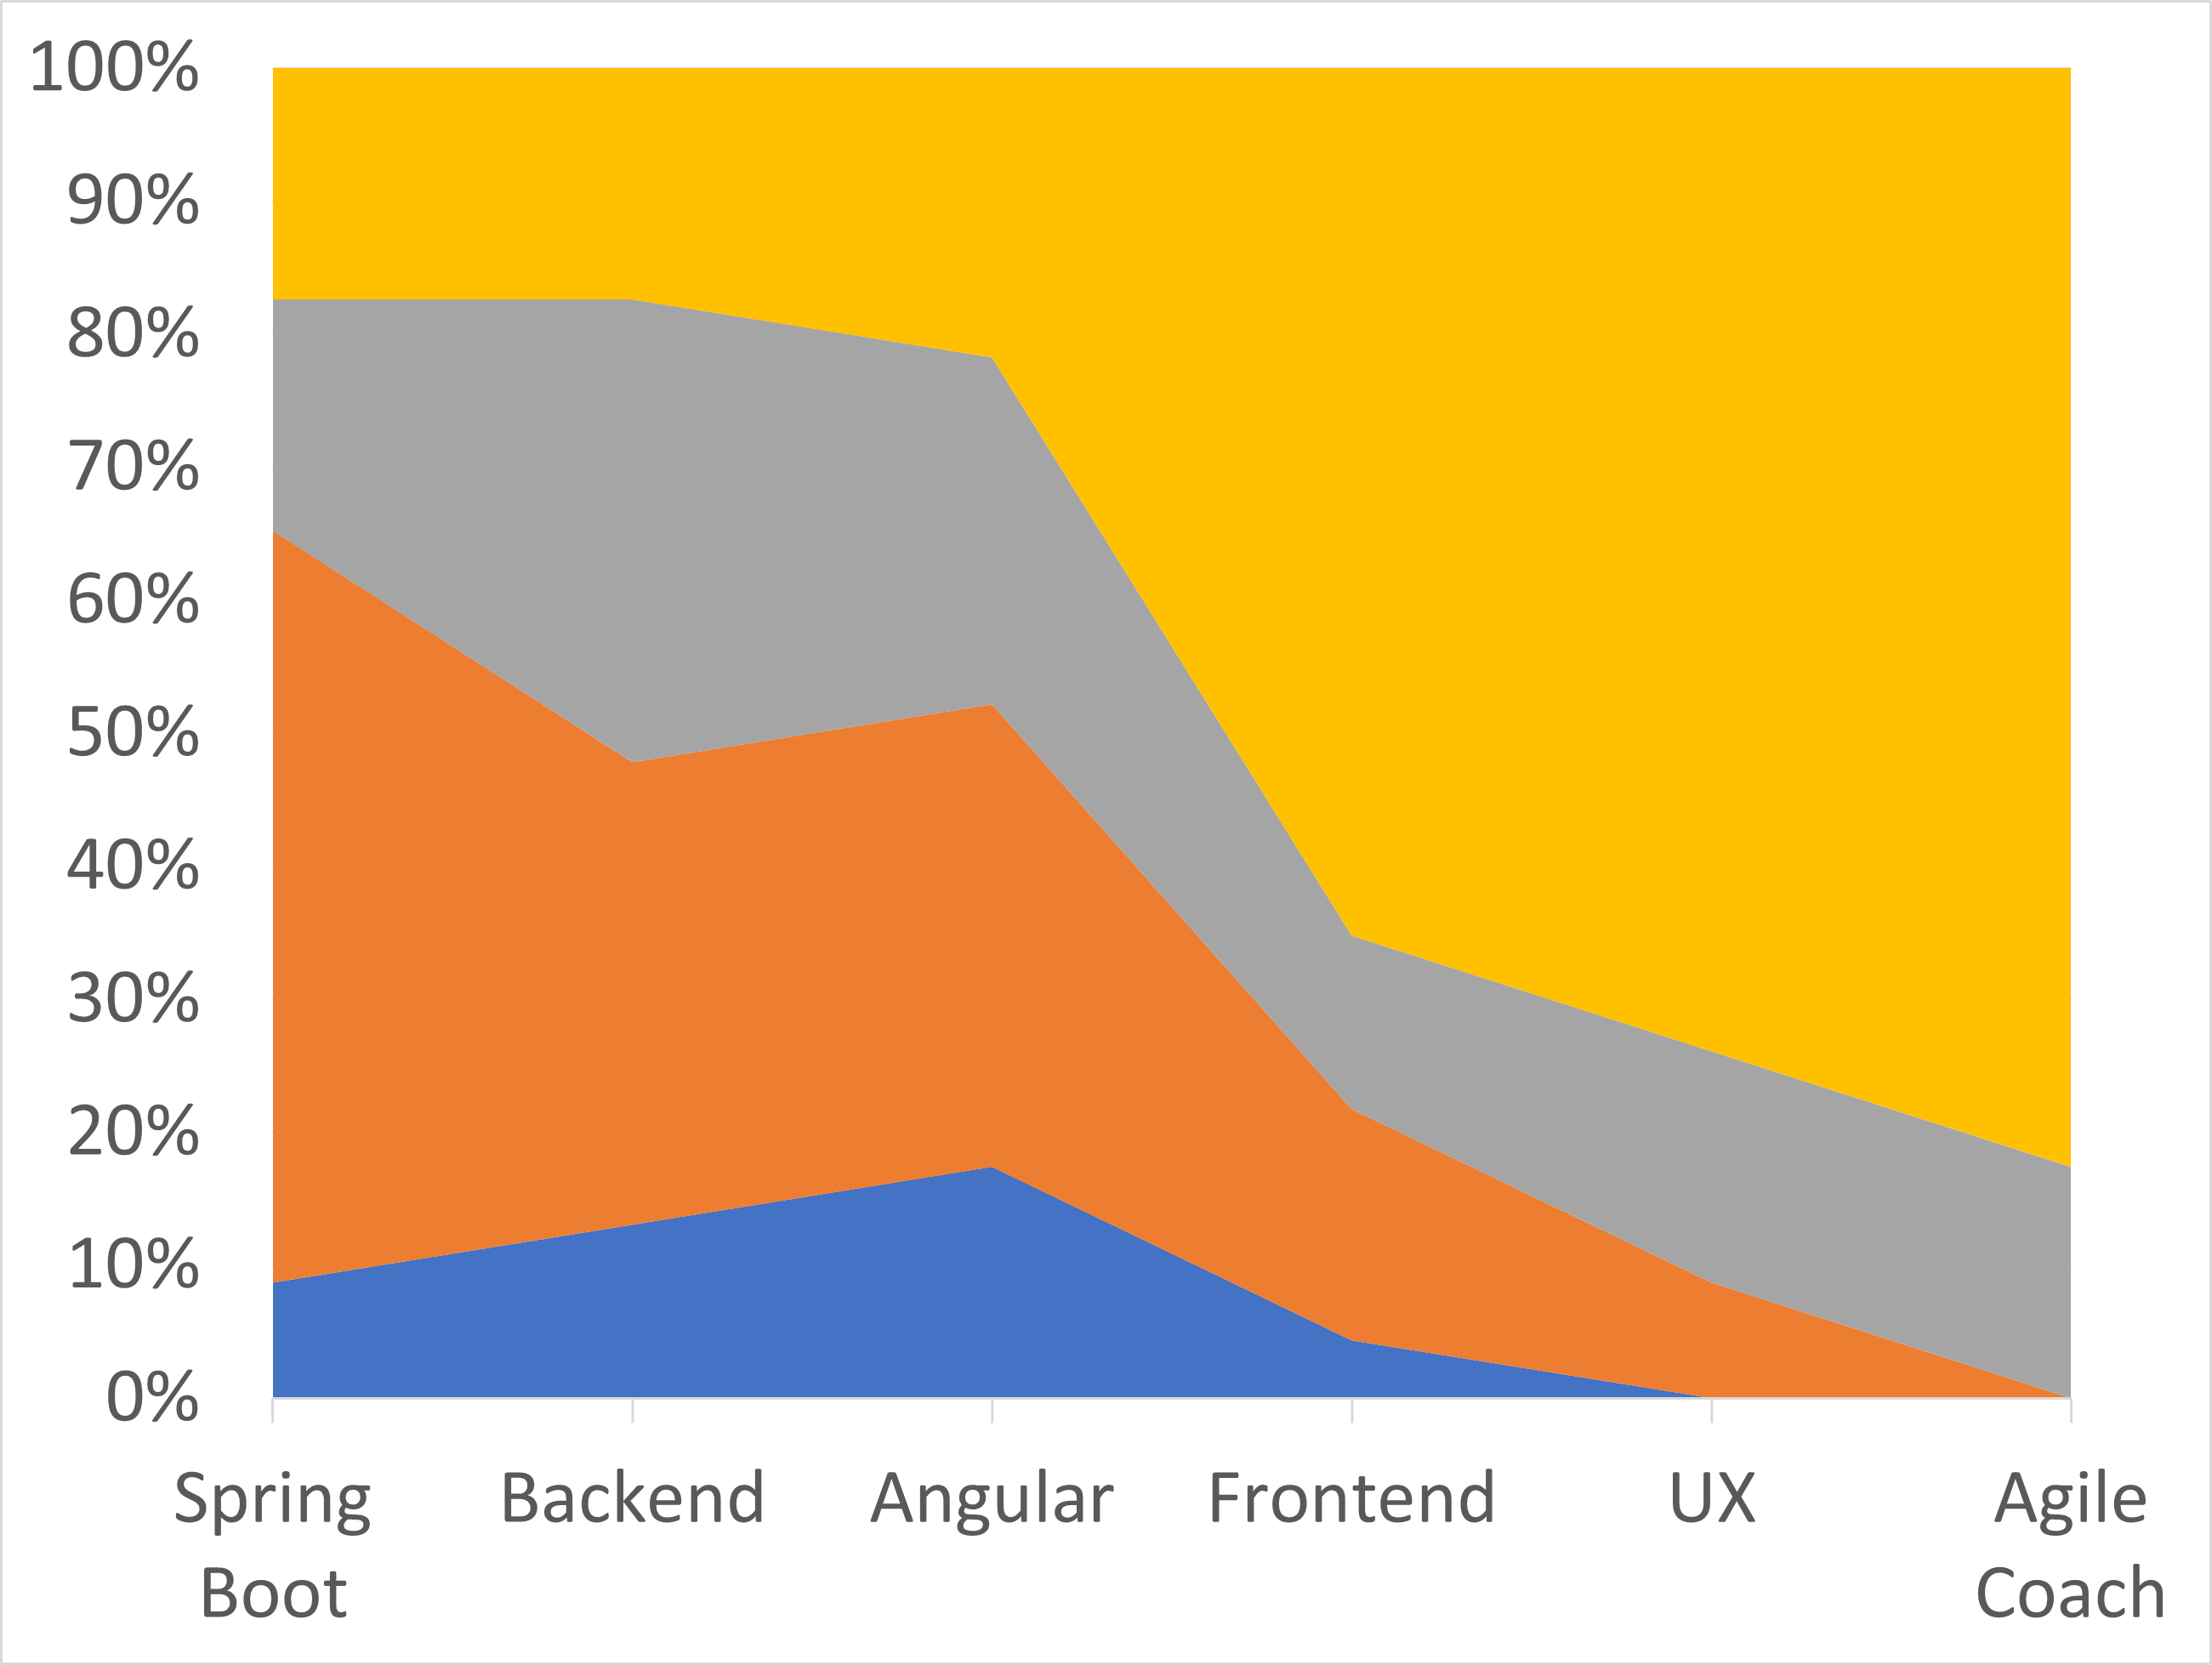
\includegraphics[width = 0.4\textwidth]{gfx/projekt-detail-c.png}}
	\subfloat[Projektposition D]{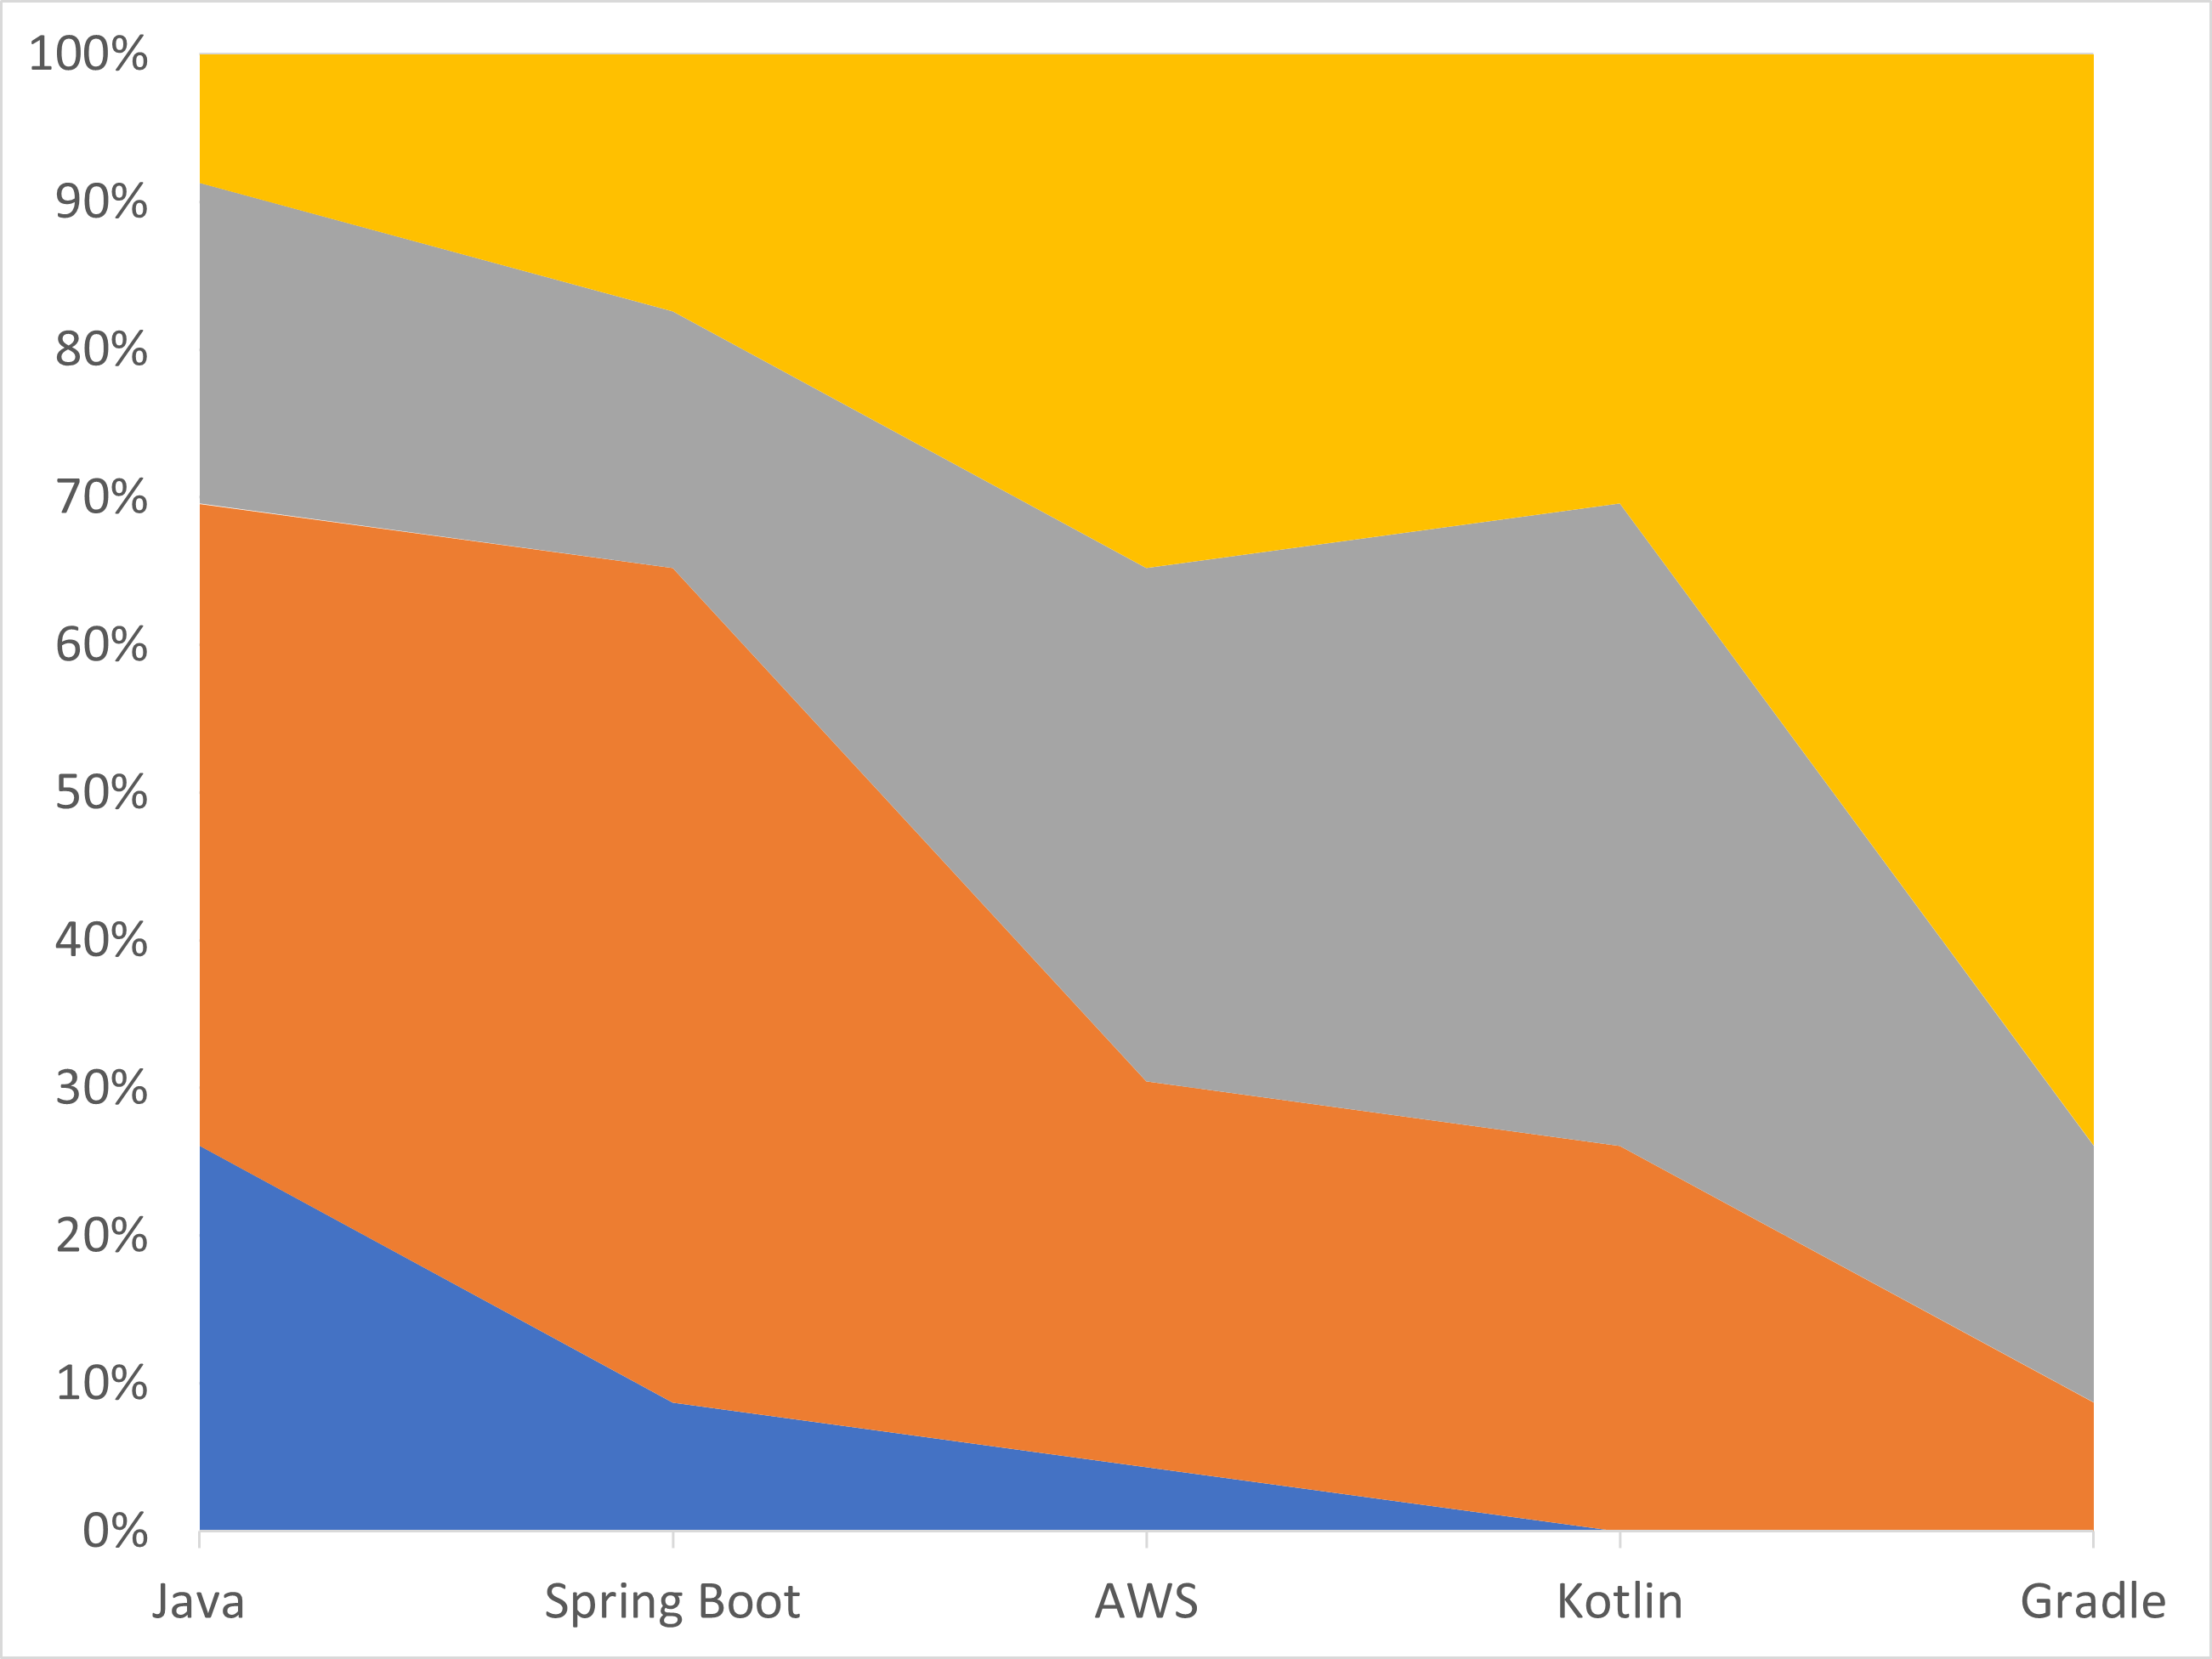
\includegraphics[width = 0.4\textwidth]{gfx/projekt-detail-d.png}}
	
\end{figure}
\begin{figure}[h]
	\centering
	\ContinuedFloat
	
	\subfloat[Projektposition E]{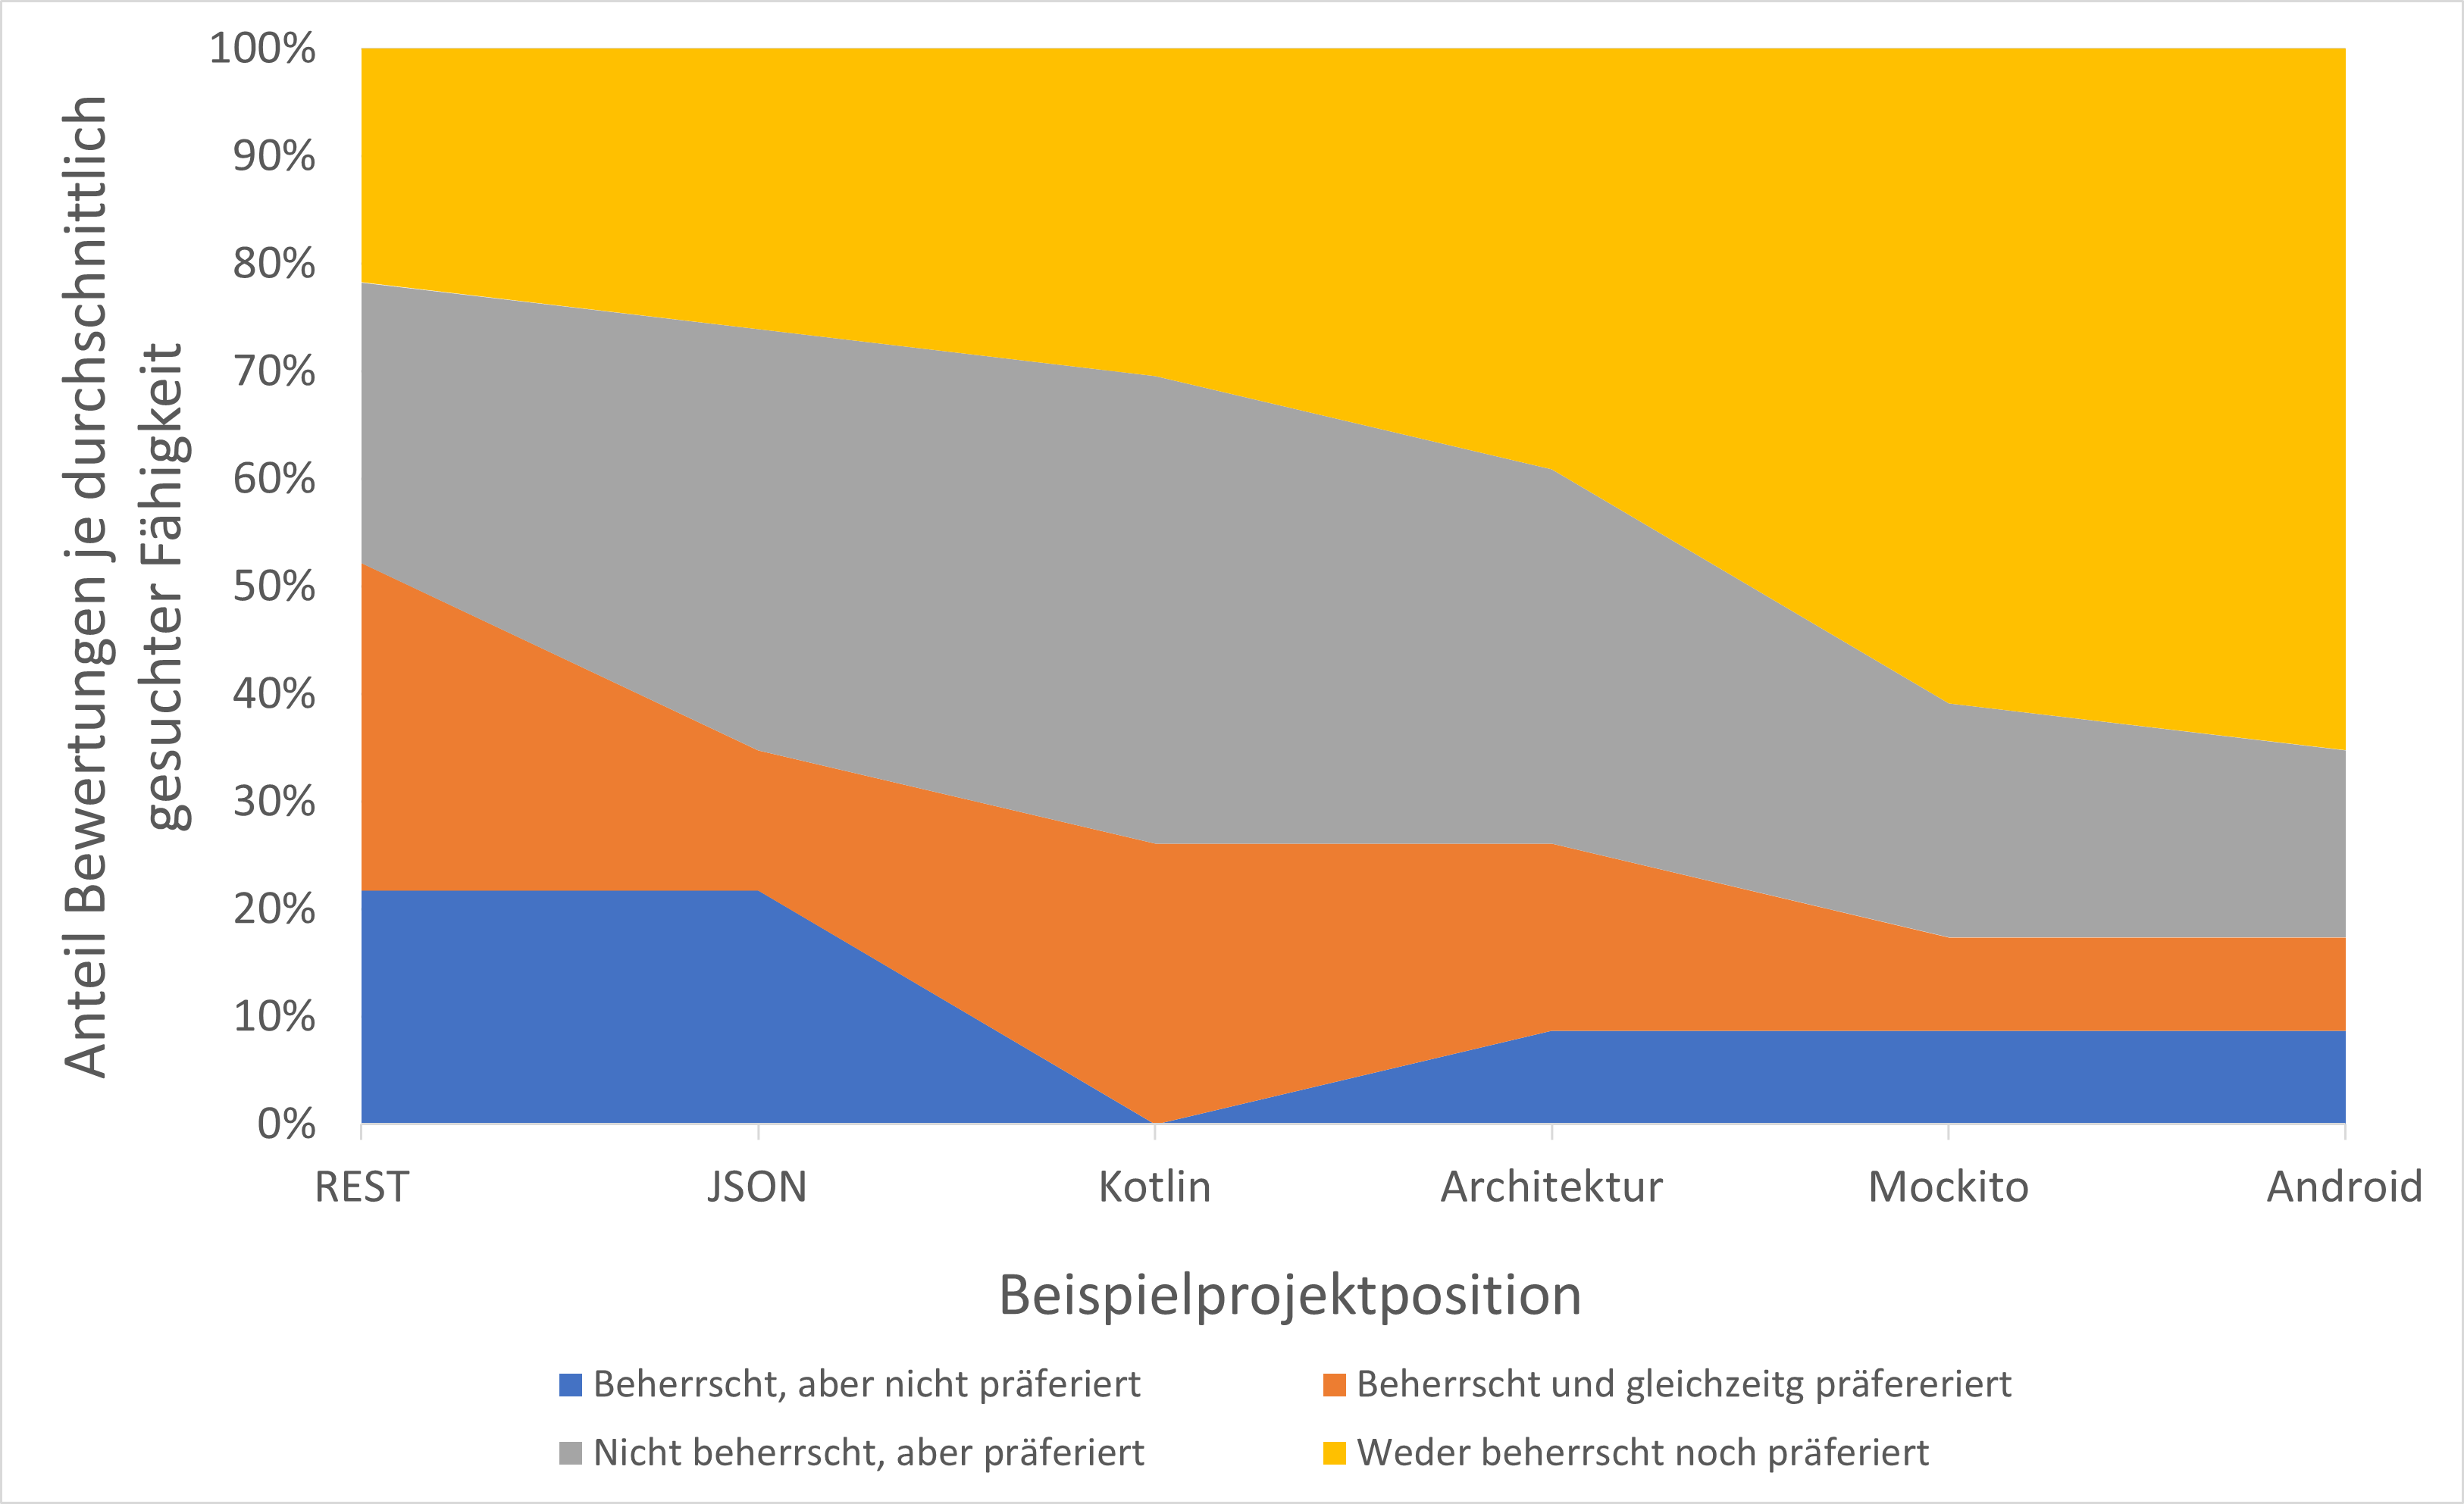
\includegraphics[width = 0.4\textwidth]{gfx/projekt-detail-e.png}}
	\subfloat[Legende]{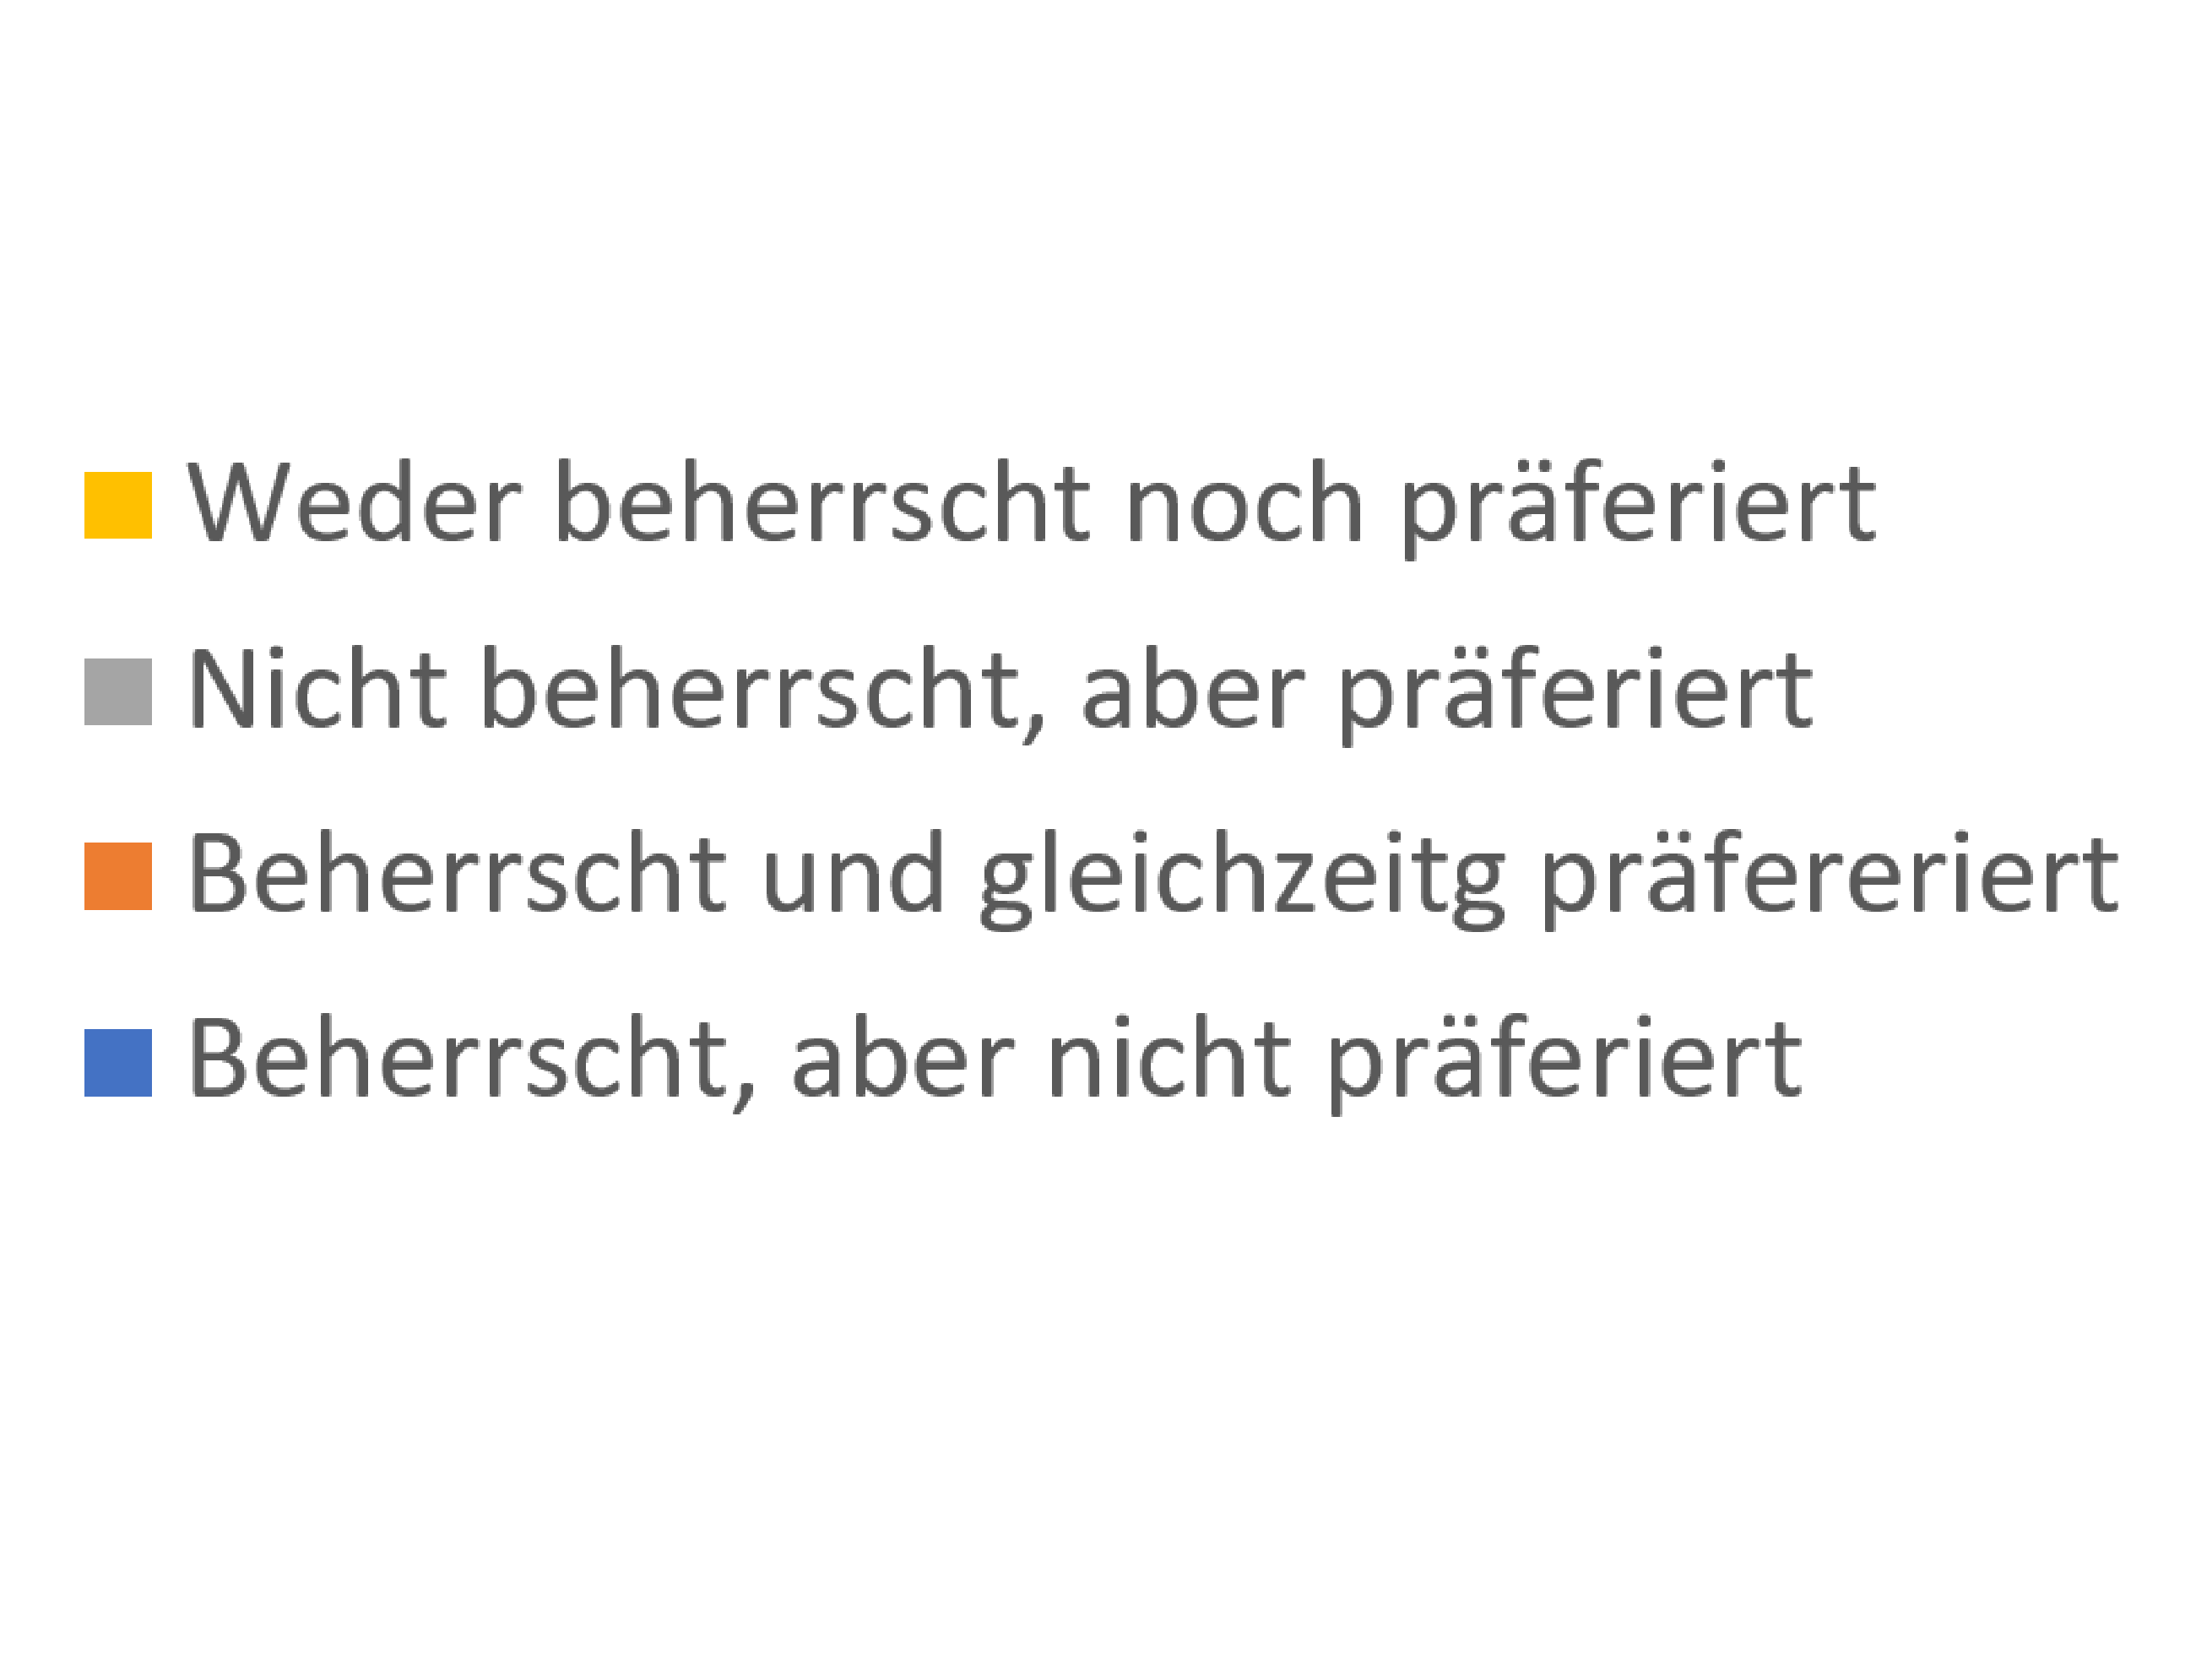
\includegraphics[width = 0.4\textwidth]{gfx/projekt-detail-legende.png}}
	
	\caption{Anteil an Mitarbeitern, welche die in den jeweiligen Beispielprojektpositionen gesuchten Fähigkeiten beherrschen bzw. präferieren}
\label{fig:ergebnisse:analyse:abb6}
\end{figure}

In Abbildung \ref{fig:ergebnisse:analyse:abb6} ist zu erkennen, dass im Durchschnitt 31 Prozent der gesuchten Fähigkeiten jedes Projekts von mindestens der Hälfte aller Mitarbeiter beherrscht werden. Für die übrigen 69 Prozent der Kompetenzen ist anschließend ein zumeist lineares Absinken der Angestellten zu beobachten, welche über diese Fähigkeiten verfügen. Wie stark die Abnahme ist, unterscheidet sich zwischen den einzelnen Projektpositionen stark. So beherrschen bei Projektposition E 17 Prozent aller Mitarbeiter mindestens eine Fähigkeit. Bei den Projektpositionen A und C werden dagegen 17 Prozent der gesuchten Fähigkeiten von keinem einzigen Angestellten beherrscht. In den Grafiken aus Abbildung \ref{fig:ergebnisse:analyse:abb6} ist außerdem zu beobachten, dass keine Kompetenz gesucht wird, welche kein einziger Angestellter in der Umfrage als Präferenz angegebene hat.

\section{Ergebnisse der Fallstudie}
\label{ch:ergebnisse:fallstudie}

\subsection{Erwartete Zufriedenheit der Projektmitarbeiter}
\label{ch:ergebnisse:fallstudie:umfrageMitarbeiter}
In der in Kapitel \ref{ch:methodik:evaluation} vorgestellten Umfrage wurde erhoben, welche Zufriedenheit die Mitarbeiter der EXXETA AG mit Tätigkeiten auf den Projektpositionen aus Abbildung \ref{fig:methodik:evaluation:abb2} prognostizieren. Die Ergebnisse sind in Tabelle \ref{tbl:ergebnisse:umfrageMitarbeiter:zufriedenheit:tbl1} dargestellt.%Dort sind unter "zufrieden" die Antwortmöglichkeiten "voll und ganz zufrieden" und "eher zufrieden" und unter "unzufrieden" die Optionen "weniger zufrieden" und "gar nicht zufrieden" zusammengefasst.

\begin{table}[h]
	\centering
	\begin{tabularx}{\textwidth}{X|X|X|X|X}
		\textbf{Projekt-position} & \textbf{Gar nicht zufrieden} & \textbf{Weniger zufrieden} & \textbf{Eher zufrieden} & \textbf{Voll und ganz zufrieden}\\ 
		\hline
		A & 4  & 4  & 10 & 5\\
		B & 3  & 6  & 7  & 7\\
		C & 10 & 7  & 4  & 2\\
		D & 5  & 7  & 7  & 4\\
		E & 5  & 10 & 4  & 4
	\end{tabularx}
	\caption{Anzahl an Mitarbeitern, welche zufrieden bzw. unzufrieden mit der Tätigkeit auf den jeweiligen Beispielprojektpositionen wären}
	\label{tbl:ergebnisse:umfrageMitarbeiter:zufriedenheit:tbl1}
\end{table}

In Tabelle \ref{tbl:ergebnisse:umfrageMitarbeiter:zufriedenheit:tbl1} ist zu erkennen, dass die Mitarbeiter überwiegend eine hohe Zufriedenheit mit den Projektpositionen A und B prognostizieren. Mit einer Tätigkeit auf den Projektpositionen C und E zeigen sich die Angestellten eher unzufrieden. Projektposition D stehen die Mitarbeiter gespalten gegenüber, sodass etwa die Hälfte der Befragten zufrieden und die andere Hälfte unzufrieden mit dieser Tätigkeit wäre.

Abbildung \ref{fig:ergebnisse:analyse:abb7} zeigt, für wie viele der 23 befragten Mitarbeiter der bilaterale Empfehlungsansatz gegenüber dem unilateralen Vorgehen für eine höhere Zufriedenheit seitens der Mitarbeiter sorgte. Wie in Kapitel \ref{ch:methodik:evaluation} beschrieben, entsteht eine höhere Zufriedenheit mit den Projekttätigkeiten, wenn das bilaterale System die Angestellten bei einer prognostizierten Zufriedenheit höher und bei einer erwarteten Unzufriedenheit niedriger positioniert als die unilaterale Anwendung.

\begin{figure}[h]
	\centering
	
	\subfloat[Projektposition A]{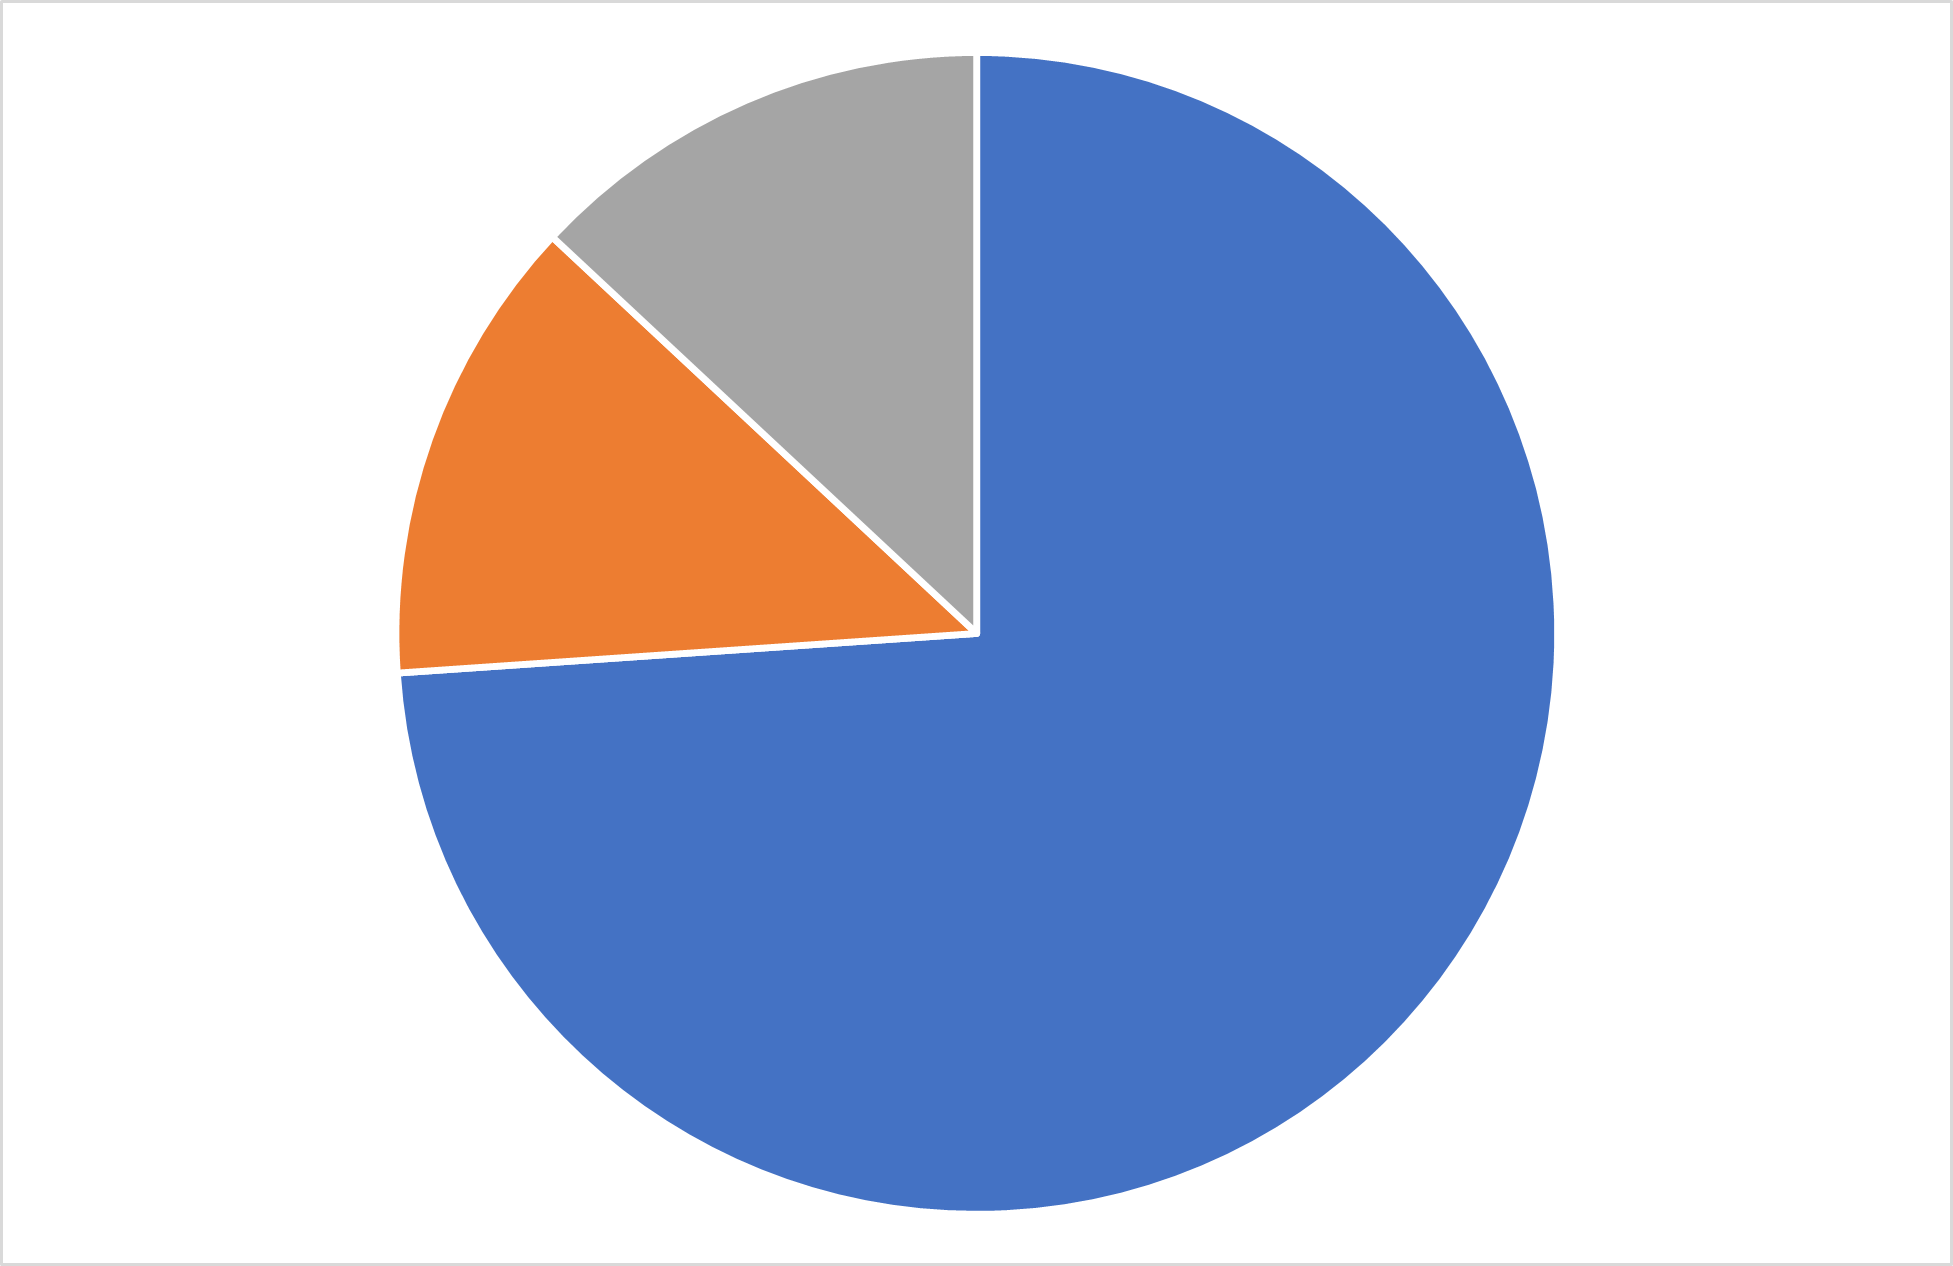
\includegraphics[width = 0.4\textwidth]{gfx/zufriedenheit-projekt-a.png}}
	\subfloat[Projektposition B]{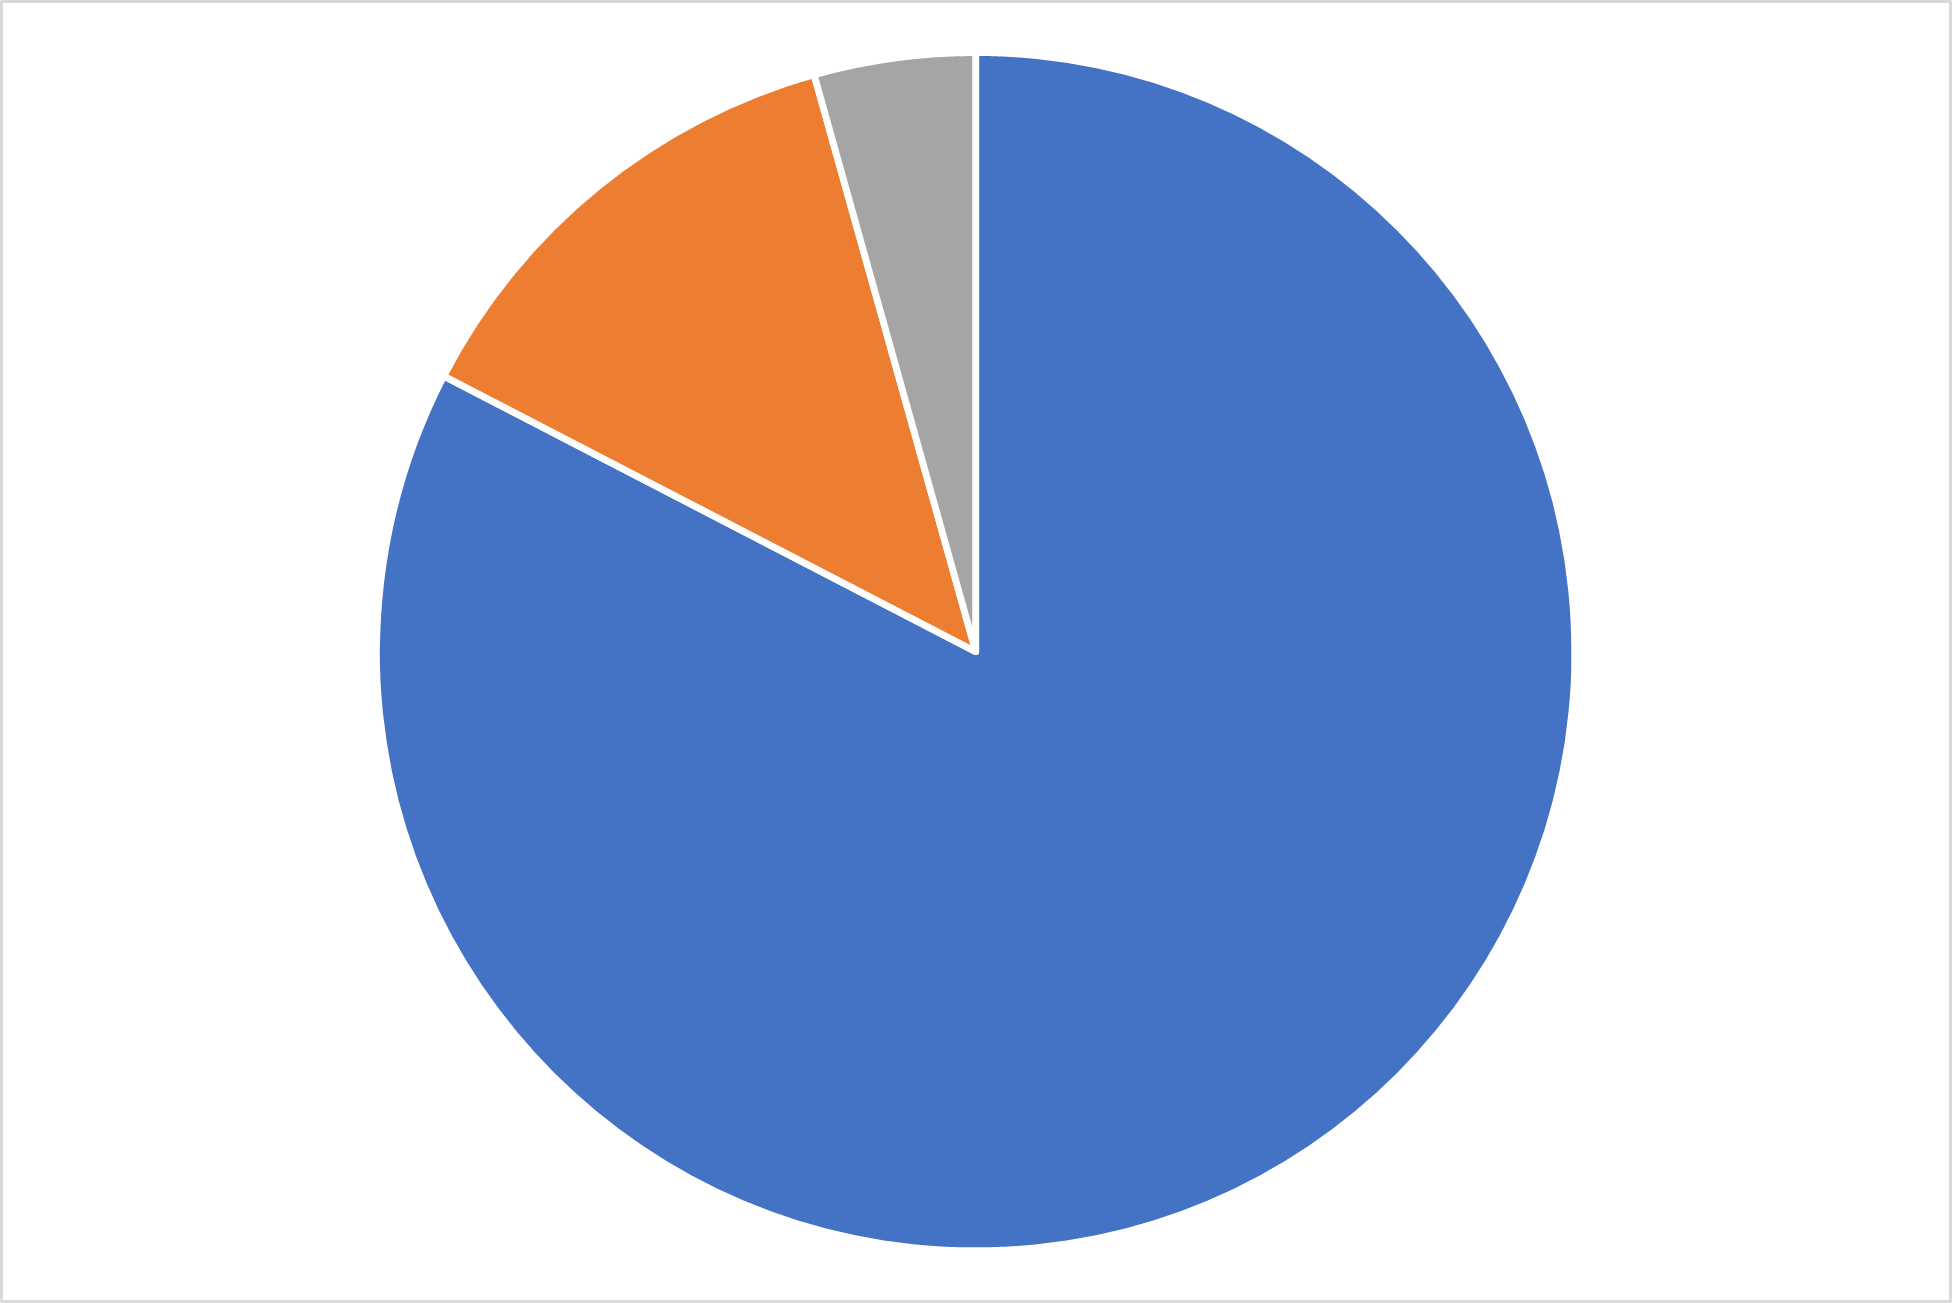
\includegraphics[width = 0.4\textwidth]{gfx/zufriedenheit-projekt-b.png}}
	\newline
	\subfloat[Projektposition C]{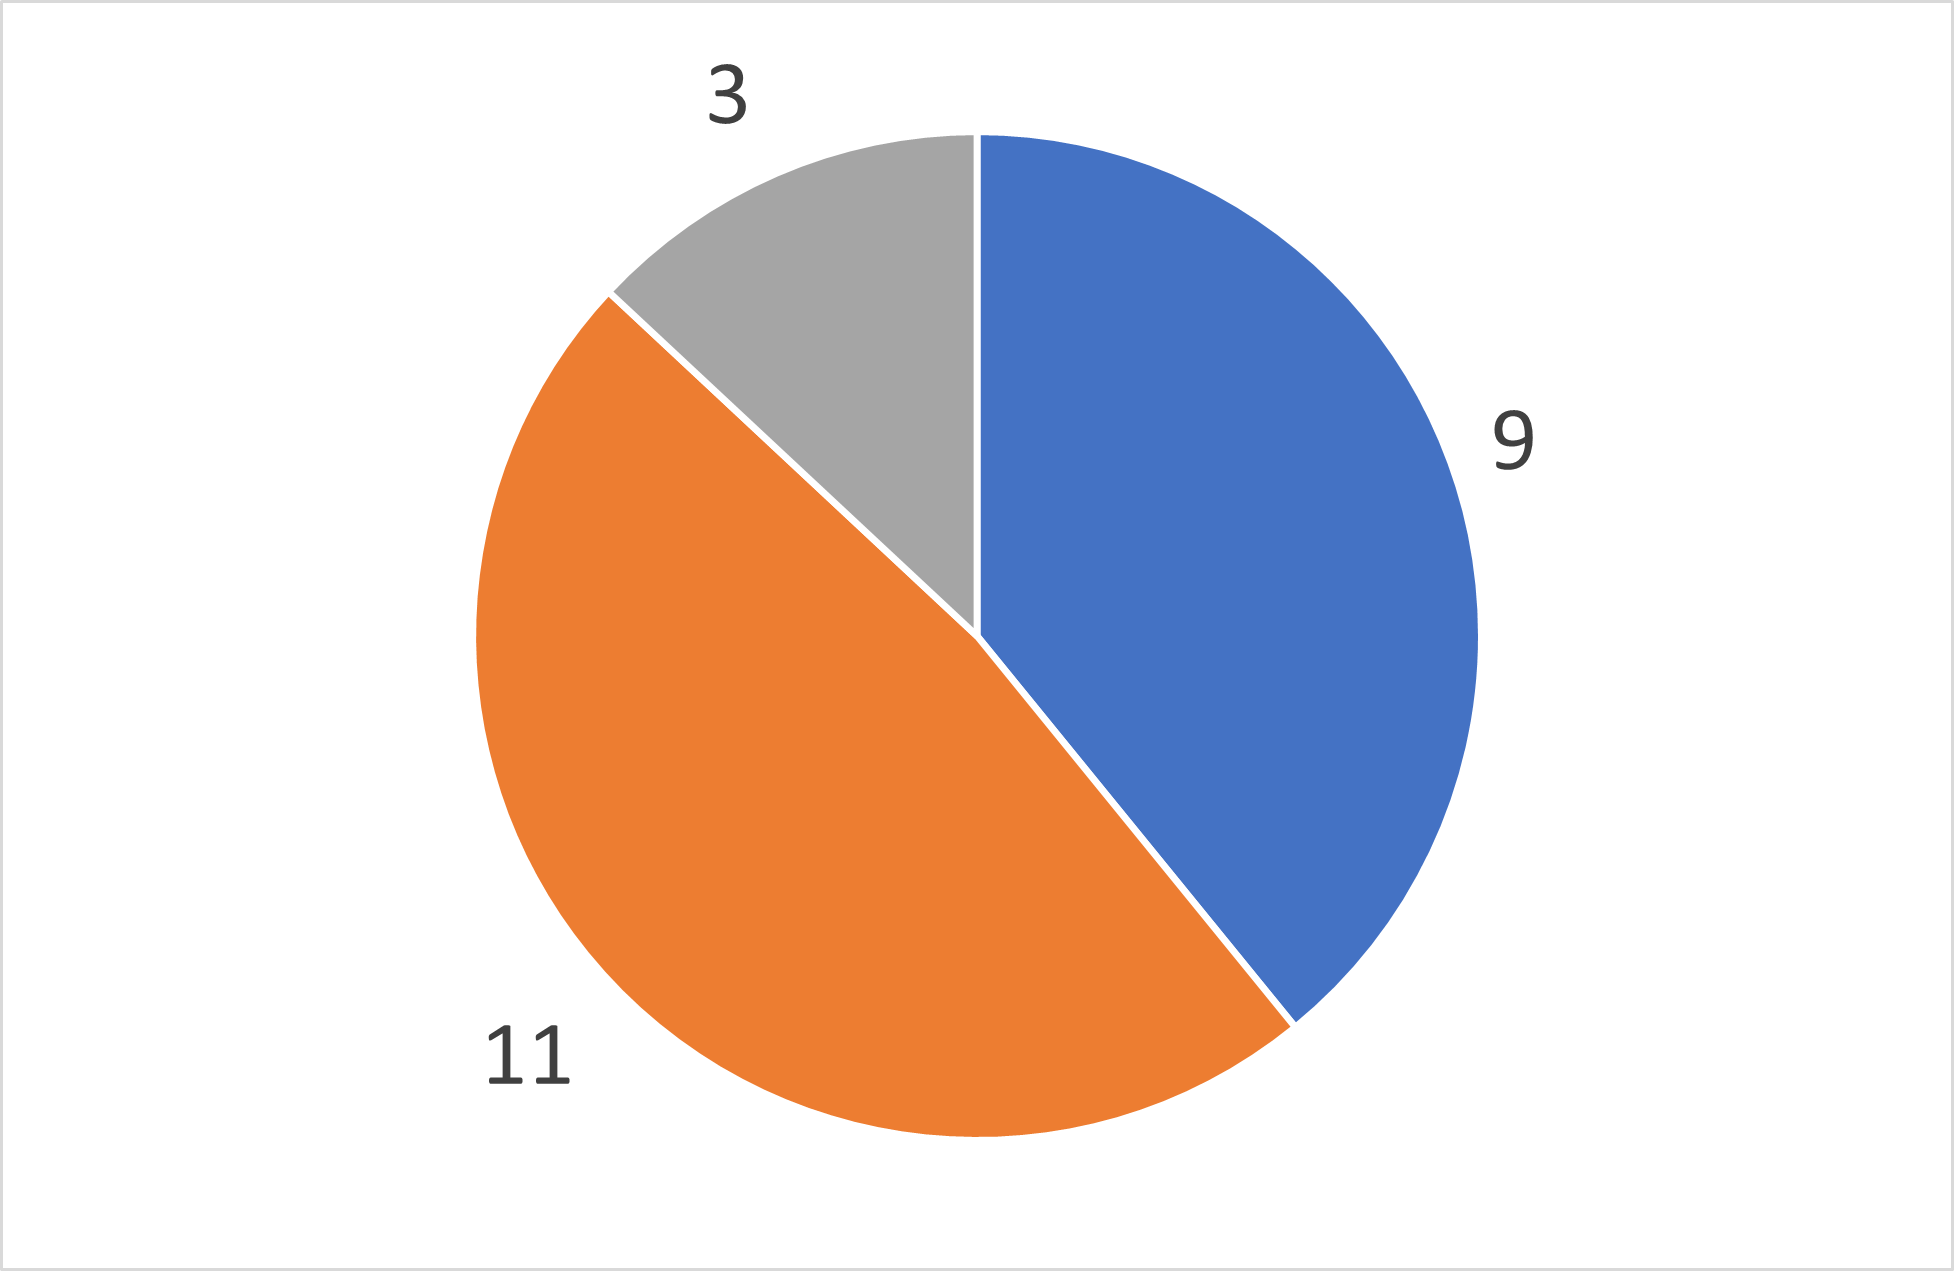
\includegraphics[width = 0.4\textwidth]{gfx/zufriedenheit-projekt-c.png}}
	\subfloat[Projektposition D]{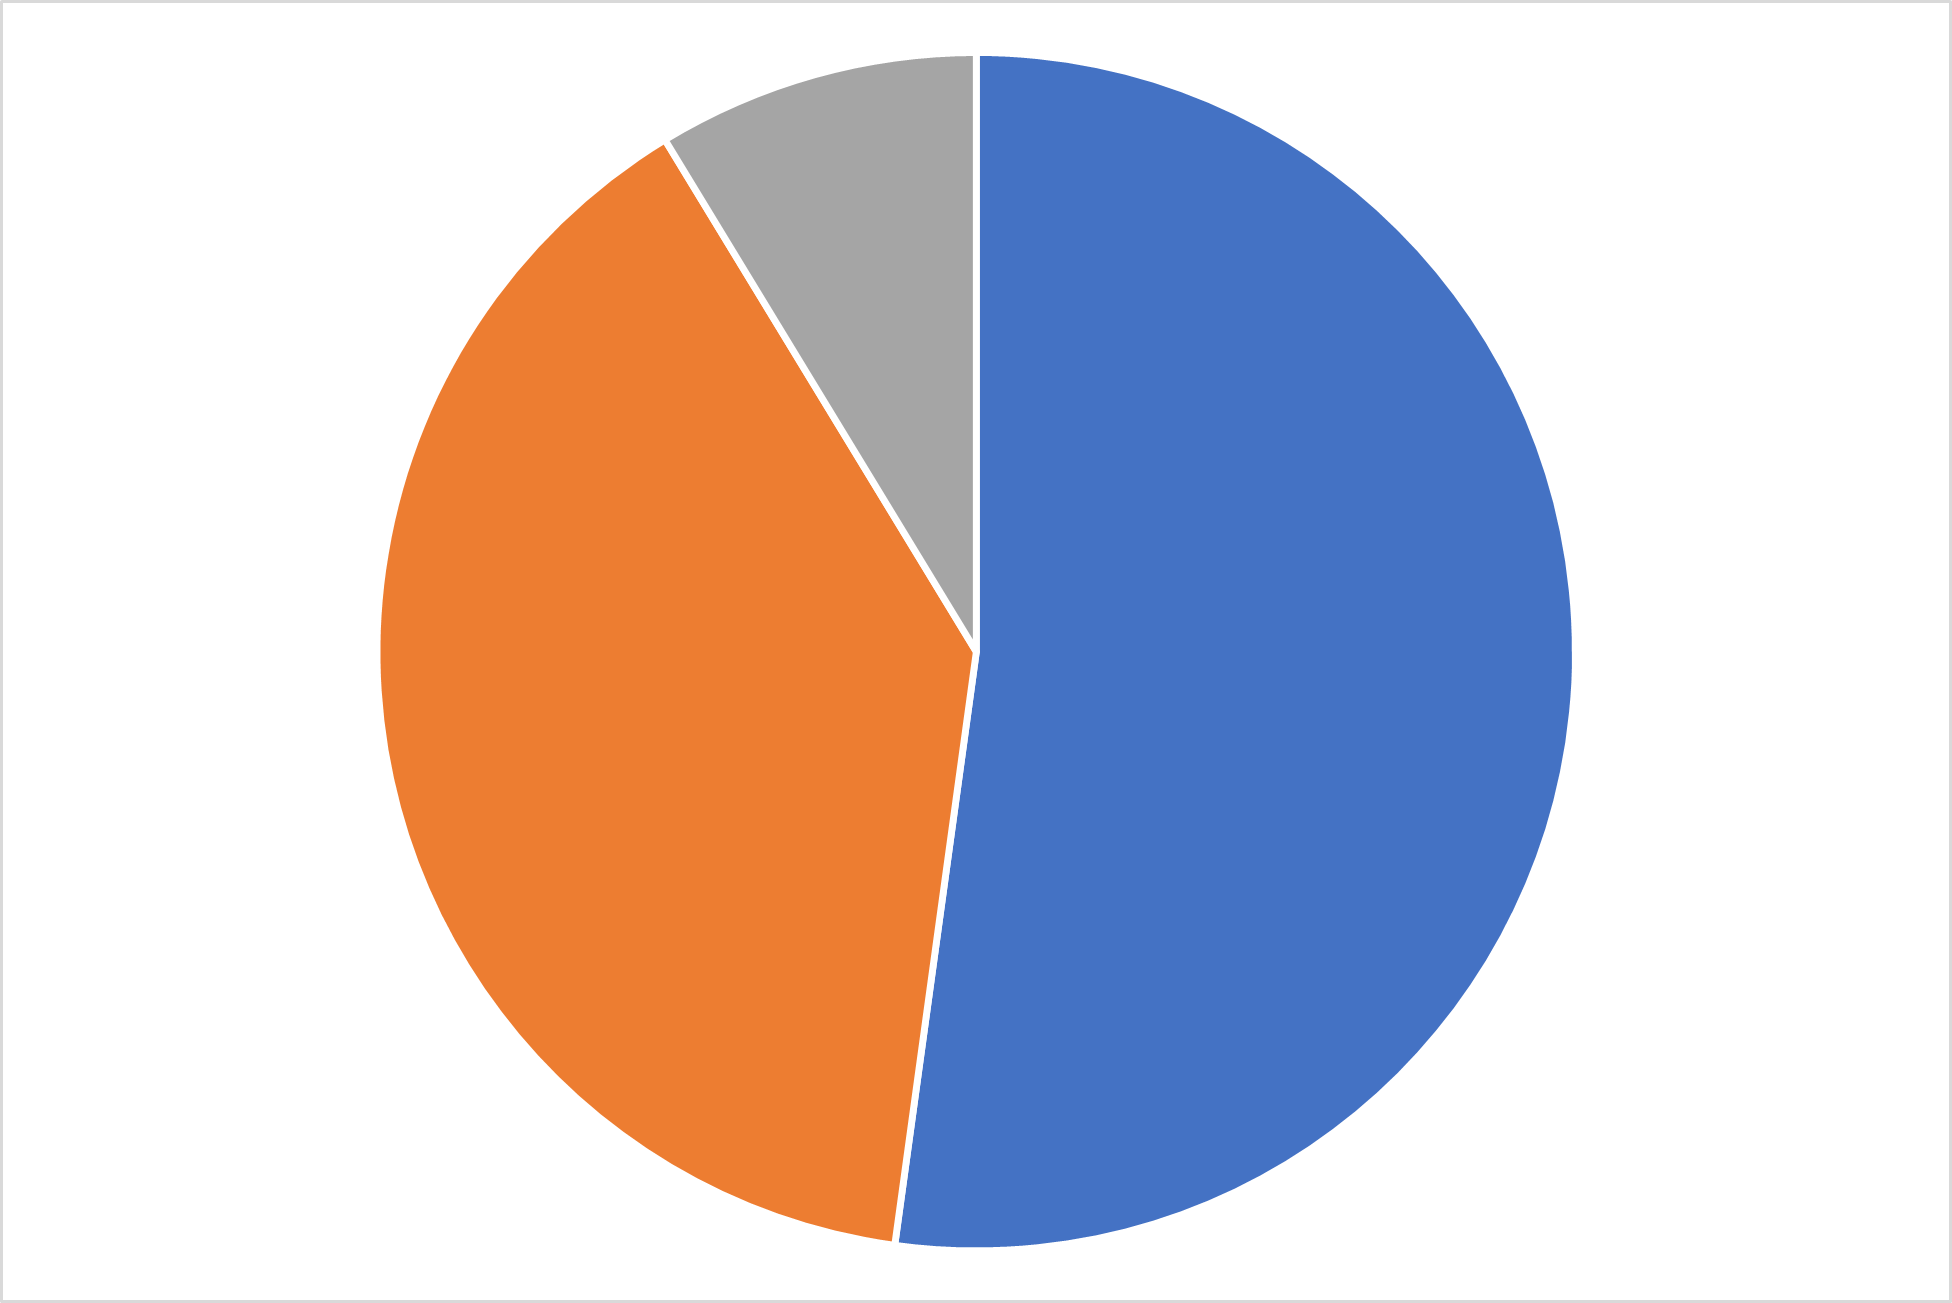
\includegraphics[width = 0.4\textwidth]{gfx/zufriedenheit-projekt-d.png}}
	\newline
	\subfloat[Projektposition E]{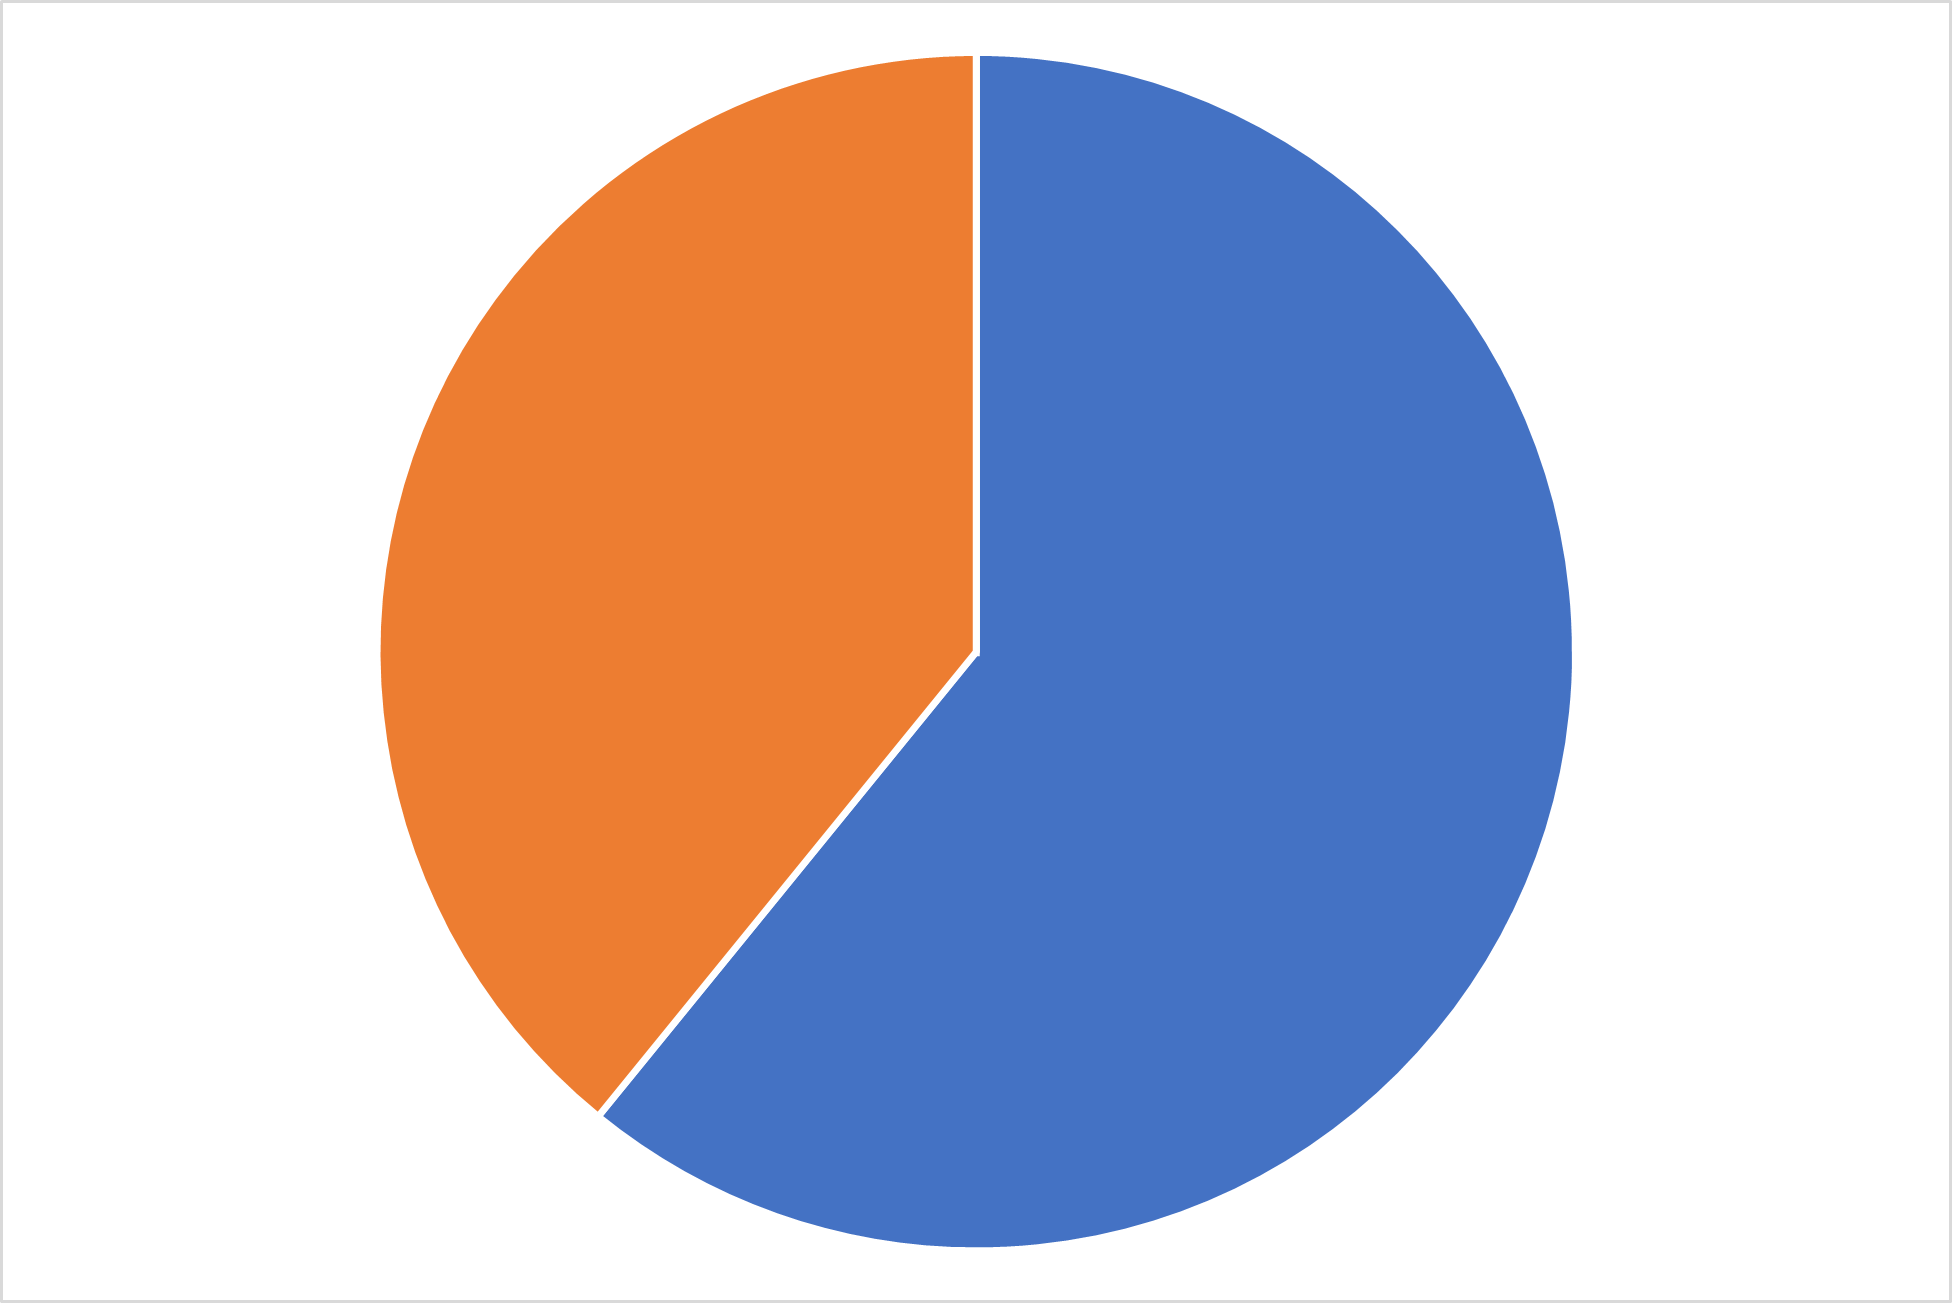
\includegraphics[width = 0.4\textwidth]{gfx/zufriedenheit-projekt-e.png}}
	\subfloat[Legende]{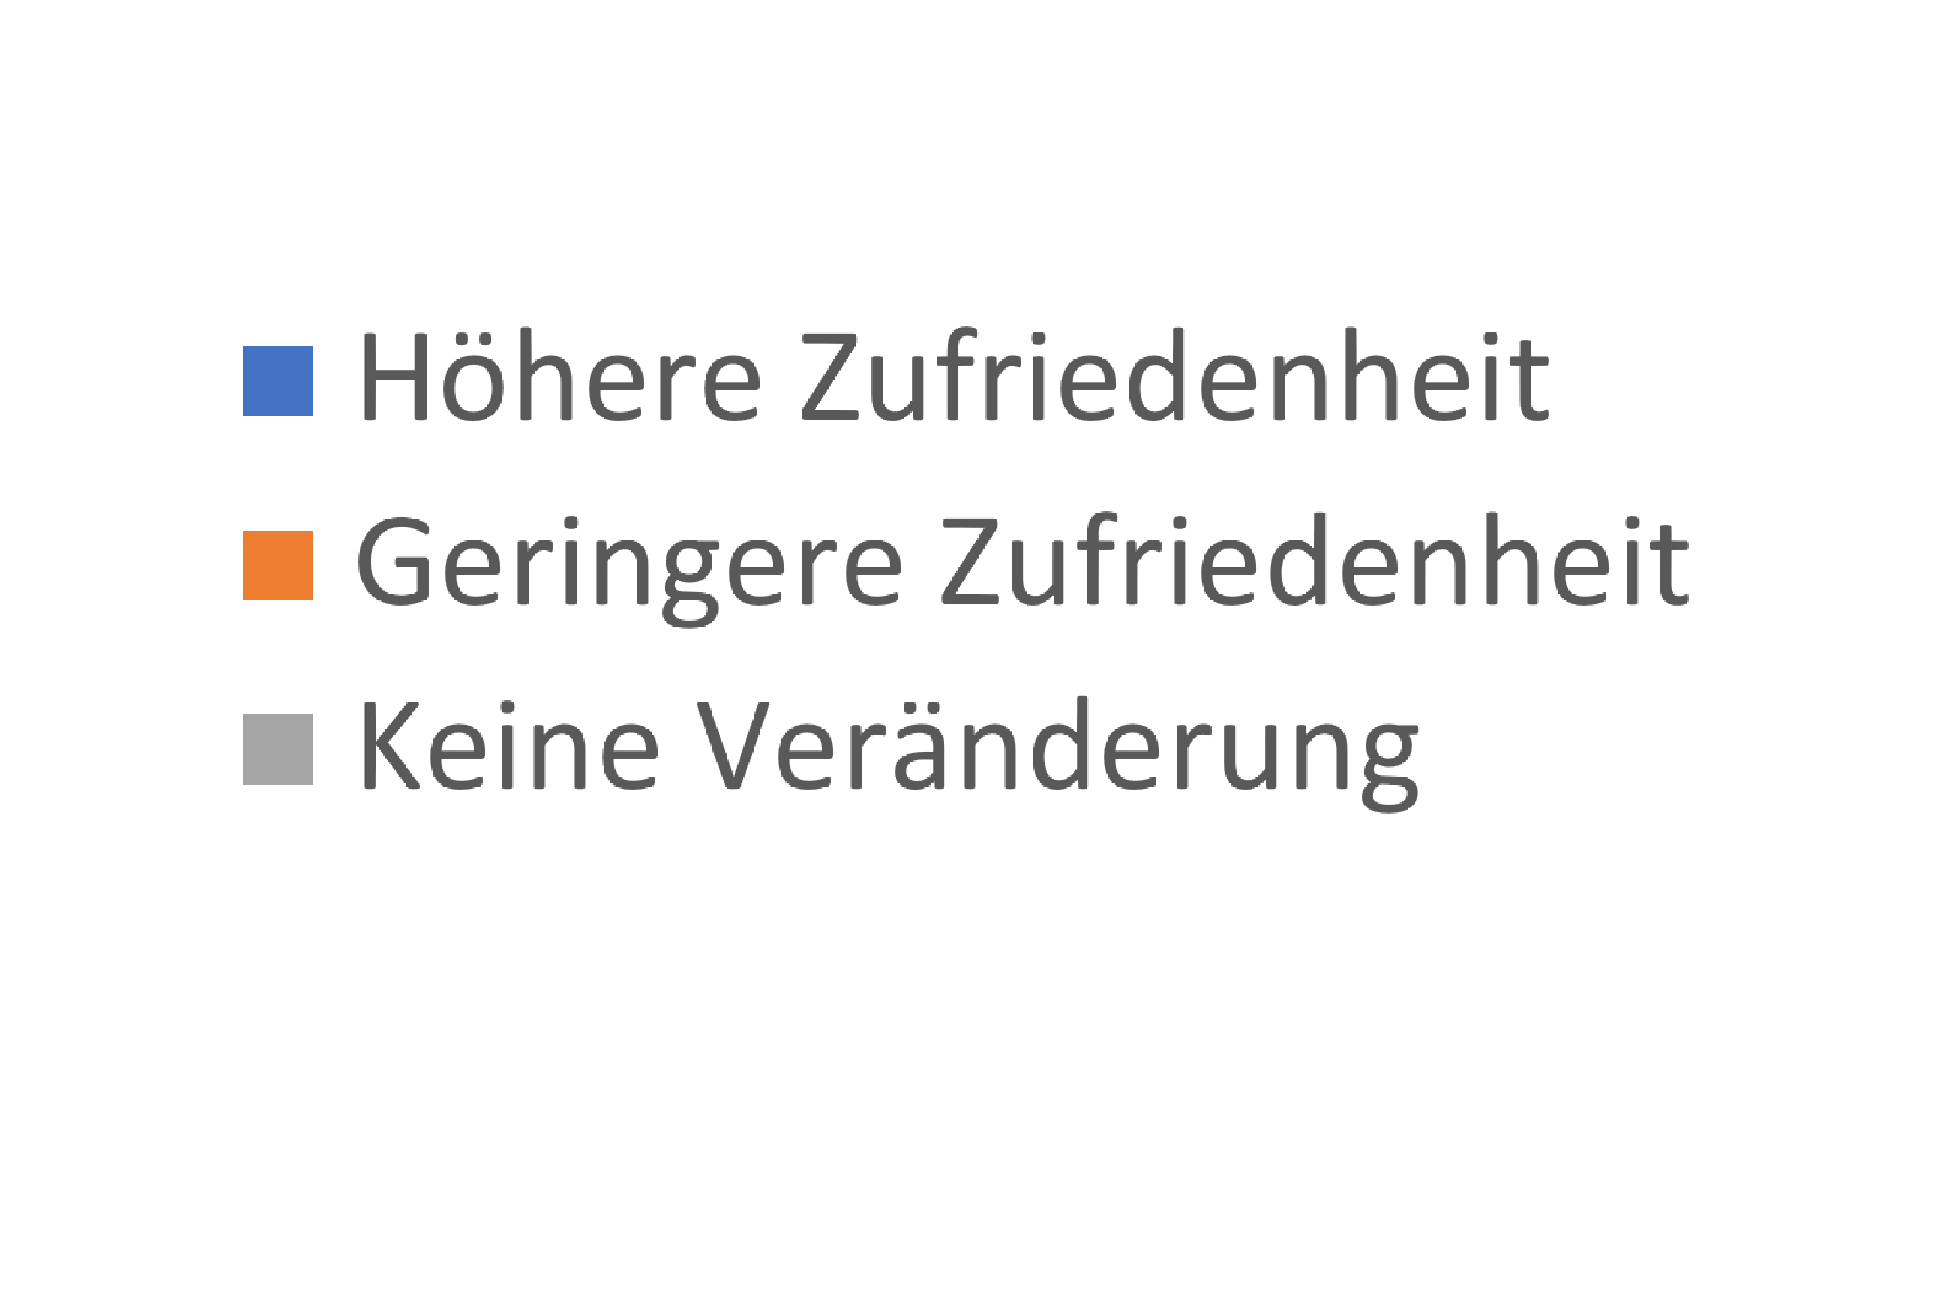
\includegraphics[width = 0.4\textwidth]{gfx/zufriedenheit-projekt-legende.png}}
	
	\caption{Ergebnisse des bilateralen Empfehlungsansatzes im Vergleich zum unilateralen Vorgehen hinsichtlich der Mitarbeiterzufriedenheit}
	\label{fig:ergebnisse:analyse:abb7}
\end{figure}

In Abbildung \ref{fig:ergebnisse:analyse:abb7} ist zu erkennen, dass der bilaterale Empfehlungsansatz einen Großteil der Angestellten für die Projektpositionen A und B zugunsten einer höheren Zufriedenheit positionierte. Bei den Projektpositionen D und E sind erreiche das bilaterale Vorschlagsverfahren für knapp über die Hälfte der Mitarbeiter eine höhere Zufriedenheit. Bei Projektposition C konnte dagegen der unilaterale Empfehlungsansatz für den Großteil der Angestellten eine höhere Zufriedenheit erzielen.

\subsection{Prognostizierte Arbeitsleistung der Projektmanager}
\label{ch:ergebnisse:fallstudie:arbeitsleistung}
\shorthandon{"}

\shorthandoff{"}
\chapter{Diskussion}
\label{ch:diskussion}

\section{Zusammenfassung der Forschungsergebnisse}
\label{ch:diskussion:zusammenfassung}
Im Rahmen der vorliegenden Master-Thesis wurde eine Fallstudie unter Projektmanagern und Mitarbeitern des IT-Beratungsunternehmens \mbox{EXXETA AG} durchgeführt. Dabei wurden die Vorschläge zur Besetzung offener Projektpositionen eines uni- und eines bilateralen Empfehlungsansatzes miteinander verglichen. Das bilaterale Vorschlagsverfahren konnte bei vier der fünf evaluierten Stellen eine höhere Zufriedenheit bei den Angestellten erzielen. Bei einer Projektposition sorgte dagegen der unilaterale Empfehlungsansatz für eine höhere Zufriedenheit. Vergleichbar fielen auch die Ergebnisse auf Seiten der Projektmanager aus. Hier prognostizierten die Verantwortlichen für drei der fünf Projektpositionen eine höhere Arbeitsleistung von den vorgeschlagenen Mitarbeitern des bilateralen Verfahrens. Bei zwei Stellen bewerten die Projektmanager dagegen die Arbeitsleistungen der vorgeschlagenen Angestellten der unilateralen Variante als höher.

Bei grafischer Darstellung von Präferenzen und beherrschten Fähigkeiten der befragten Mitarbeiter zeigte sich der sogenannte lange (Ratten-)Schwanz. Zudem hatten 17 Prozent der befragten Angestellten keine einzige Kompetenzbewertung im Intranet der EXXETA AG vorgenommen. Darüber hinaus konnte festgestellt werden, dass die Mitarbeiter einen Großteil ihrer präferierten Fähigkeiten nicht beherrschen. Weitere Analysen ergaben, dass etwa 28 Prozent der befragten Angestellten die durchschnittlich für eine offene Projektposition gesuchte Fähigkeit nicht als Präferenz angaben, obwohl sie diese beherrschen. 

Abschließend wurde evaluiert, wie Mitarbeiter und Projektmanager mit möglicher Unterforderung bei der Projektarbeit umgehen. Diesbezüglich konnte im Rahmen der Befragung festgestellt werden, dass sowohl Angestellte als auch Projektverantwortliche mehrheitlich eine Unterforderung vermeiden möchten.
\newpage
\section{Interpretation der Forschungsergebnisse}
\label{ch:diskussion:interpretation}
In Kapitel \ref{ch:personEnvironmentFit:auswirkungenErhoehterAngebote} wurde beschrieben, dass ein P-E Misfit in drei möglichen Konsequenzen mit entsprechenden Gleichungen zur Berechnung resultieren kann. Im Rahmen der vorliegenden Master-Thesis wurde angenommen, dass sowohl Projektmitarbeiter als auch -manager eine Unterforderung bei der Besetzung offener Projektpositionen vermeiden möchten. Dementsprechend wurde Kurve B aus Abbildung \ref{fig:personEnvironmentFit:auswirkungenErhoehterAngebote:abb1} in Form der quadrierten Differenzberechnung implementiert. Die im Rahmen der Fallstudie erhobenen Daten bestätigen diese Annahme sowohl aus Perspektive der Mitarbeiter als auch aus dem Blickwinkel der Projektverantwortlichen. 

Bei Implementierung der beiden Empfehlungsansätze wurde aufgrund der Erkenntnisse aus Kapitel \ref{ch:empfehlungssysteme} erwartet, dass sowohl der Kaltstart als auch der lange (Ratten-)Schwanz und das damit verbundene Sparsity Problem die Vorschlagserstellung beeinträchtigen würden. Daher lag den Empfehlungsmethoden ein hybrider und graphenbasierter Ansatz zugrunde, welcher über die Einbeziehung von Fähigkeitsbewertungen und Teamzuordnungen beide Probleme löste. Dieses Vorgehen ist mit Blick auf die Auswertung von beherrschten und präferierten Kompetenzen der Mitarbeiter als sinnvoll zu bewerten. Einerseits konnte in Abbildung \ref{fig:ergebnisse:analyse:abb1} der lange (Ratten-)Schwanz identifiziert werden und andererseits hatten 17 Prozent der befragten Mitarbeiter im Intranet keine einzige Fähigkeit bewertet.%Folglich wären diese Angestellten ohne Einbeziehung der Teamzuordnungen von einem Kaltstart betroffen.

Hinsichtlich der Kompetenzen konnte außerdem beobachtet werden, dass die Mitarbeiter einen Großteil ihrer präferierten Fähigkeiten nicht beherrschen. Aus diesem Sachverhalt lässt sich schließen, dass die Angestellten bereit sind, in Zukunft weitere Fähigkeiten zu erlernen und diese bei der Projektarbeit anzuwenden. Auf Unternehmensseite könnte dementsprechend der Einsatz zusätzlicher Weiterbildungsangebote evaluiert werden, bei welchen die Mitarbeiter nicht nur bestehende Kompetenzen vertiefen, sondern auch neue Fähigkeiten erlernen können.

Des weiteren zeigte die Auswertung der Mitarbeiterkompetenzen, dass das Beherrschen einer Fähigkeit keinen Rückschluss auf eine entsprechende Präferenz zulässt. Ein unilateraler Empfehlungsansatz würde dennoch sämtliche beherrschten Kompetenzen gleich behandeln. Somit ist davon auszugehen, dass die Angestellten bei Einsatz eines unilateralen Empfehlungssystems für Projektpositionen vorgeschlagen werden, deren gesuchte Fähigkeiten diese zumindest teilweise nicht anwenden möchten. Ein bilaterales System unterscheidet dagegen zwischen präferierten und nicht gewünschten Kompetenzen. Da dieser Ansatz präferierte Fähigkeiten stärker gewichtet, wird sich ein vorgeschlagener Mitarbeiter mit höherer Wahrscheinlichkeit die Anwendung der geforderten Kompetenzen wünschen. Dementsprechend ist eine höhere Zufriedenheit und Motivation bei der Stellenbesetzung zu erwarten. Diese Annahme spiegelt sich auch in den Ergebnissen der Umfragen unter den Mitarbeitern und Projektmanagern der EXXETA AG wider. Zur Verdeutlichung dieses Sachverhalts zeigt Abbildung \ref{fig:diskussion:interpretation:abb1} erneut die prognostizierte Zufriedenheit der Mitarbeiter mit den fünf vordefinierten Projektpositionen aus Kapitel \ref{ch:ergebnisse:fallstudie:umfrageMitarbeiter}.

\begin{figure}[h]
	\centering
	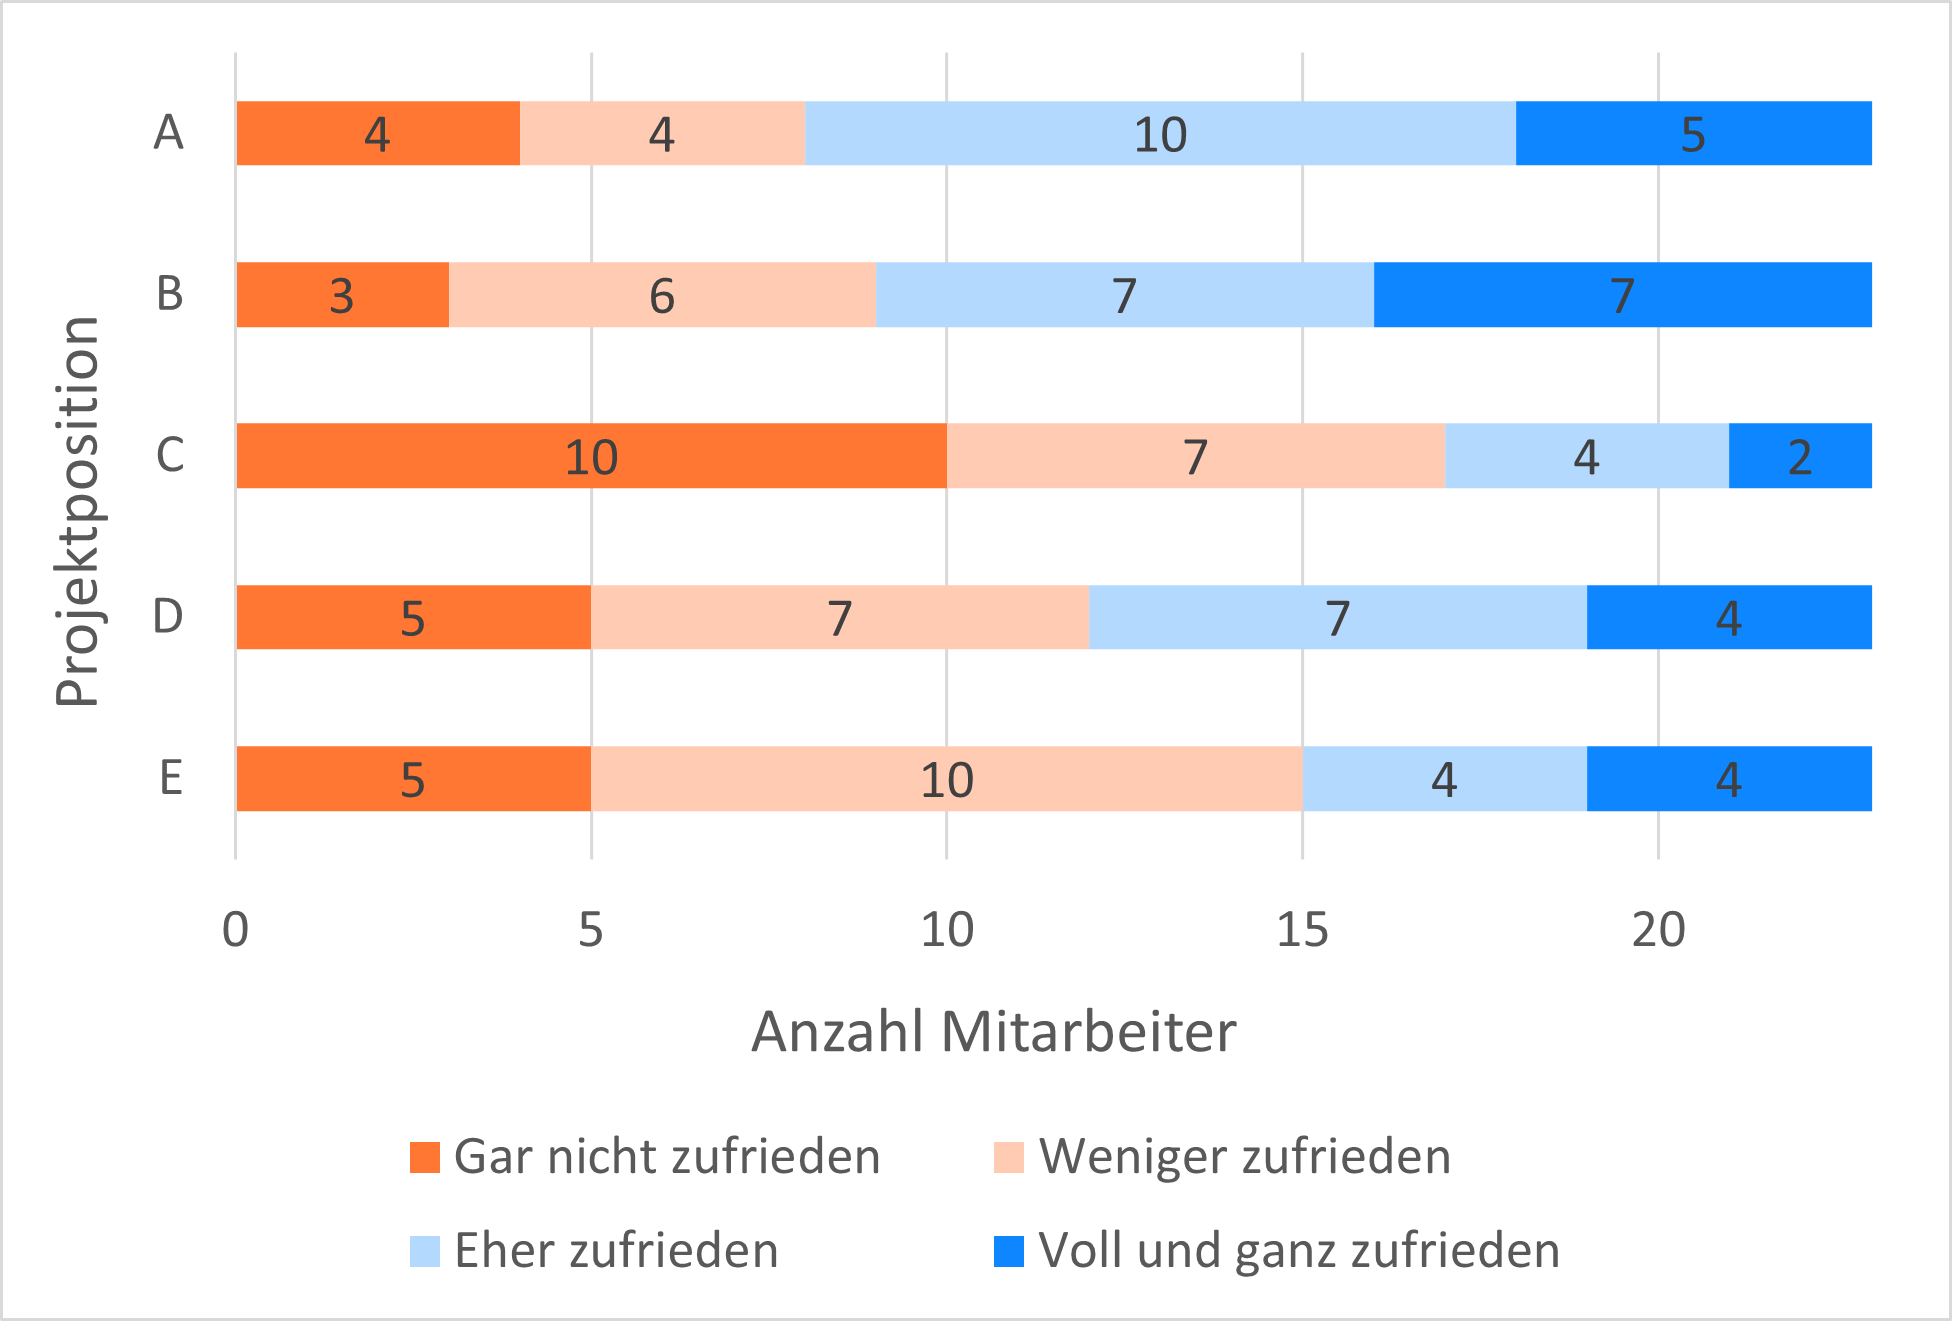
\includegraphics[width=0.925\textwidth]{gfx/mitarbeiter-zufriedenheit-umfrage.png}
	\caption{Anzahl an Mitarbeitern, welche zufrieden bzw. unzufrieden mit der Tätigkeit auf den jeweiligen vordefinierten Projektpositionen wären}
	\label{fig:diskussion:interpretation:abb1}
\end{figure}

Abbildung \ref{fig:diskussion:interpretation:abb3} veranschaulicht zusätzlich die Ergebnisse der uni- und bilateralen Empfehlungsansätze hinsichtlich der Mitarbeiterzufriedenheit. 

\begin{figure}[h]
	\centering
	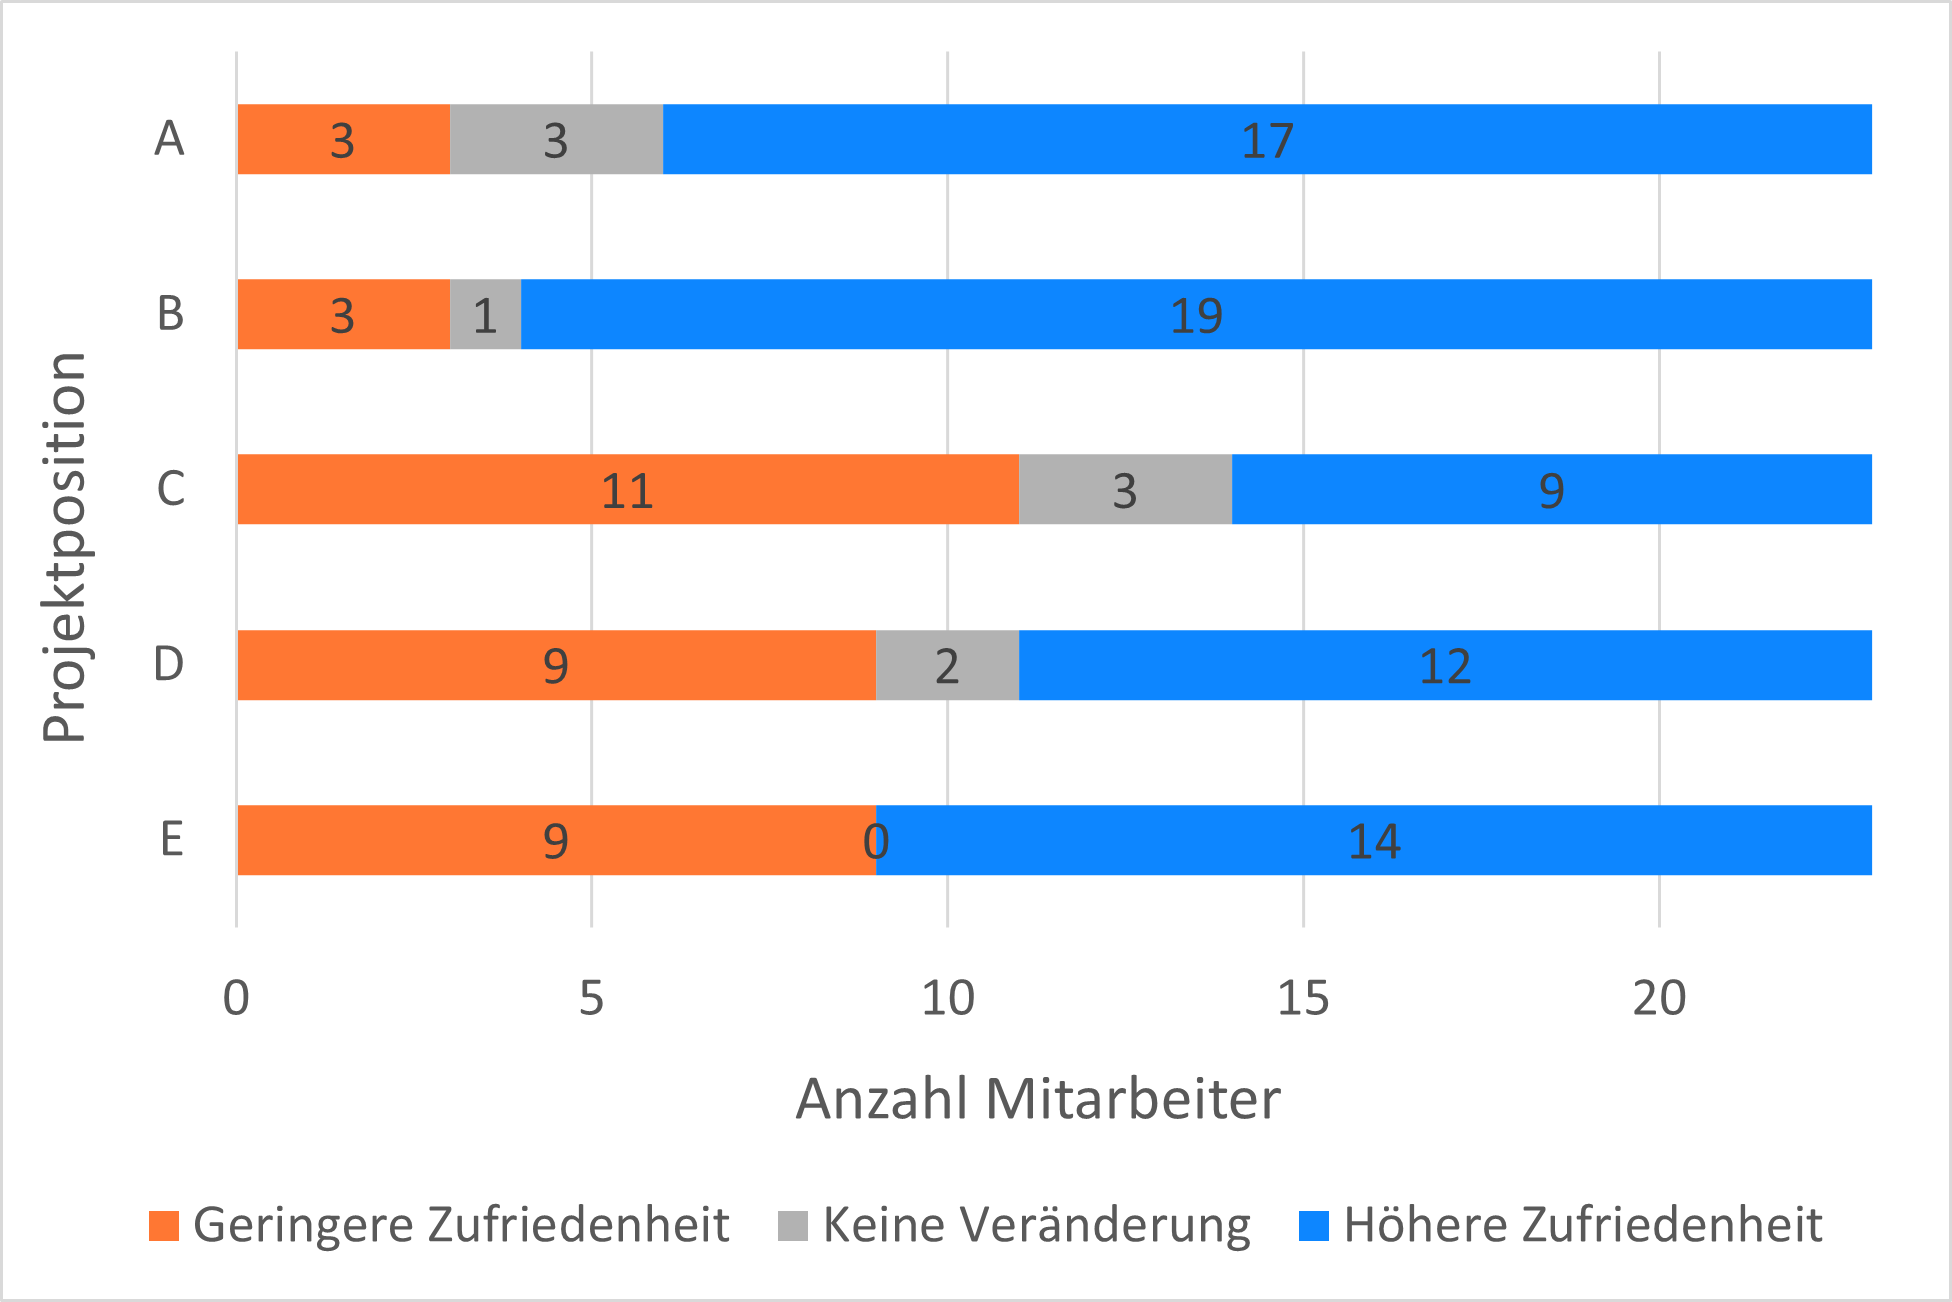
\includegraphics[width=0.925\textwidth]{gfx/zufriedenheit-projekte.png}	
	\caption{Ergebnisse des bilateralen Empfehlungsansatzes im Vergleich zum unilateralen Vorgehen hinsichtlich der Mitarbeiterzufriedenheit}
	\label{fig:diskussion:interpretation:abb3}
\end{figure}

In den Abbildungen \ref{fig:diskussion:interpretation:abb1} und \ref{fig:diskussion:interpretation:abb3} ist zu erkennen, dass die Mitarbeiter durch den bilateralen Empfehlungsansatz stärker zu deren Zufriedenheit positioniert werden, wenn sie eine hohe Akzeptanz mit der Stelle prognostizieren. Dieser Sachverhalt ist insbesondere bei den Projektpositionen A und B zu beobachten, für welche über die Hälfte der Mitarbeiter in Abbildung \ref{fig:diskussion:interpretation:abb1} eine hohe Präferenz angaben. Hier ordnete der bilaterale Empfehlungsansatz in Darstellung \ref{fig:diskussion:interpretation:abb3} etwa dreiviertel aller Angestellten gegenüber der unilateralen Variante stärker zu deren Zufriedenheit an. Zeigen dagegen weniger Mitarbeiter Gefallen an einer betrachteten Stelle, nimmt auch die Qualität des bilateralen Empfehlungsansatzes hinsichtlich der Mitarbeiterzufriedenheit ab. Besonders gut ist diese Begebenheit bei Projektposition C zu erkennen, mit welcher sich die Mitarbeiter in Abbildung \ref{fig:diskussion:interpretation:abb1} mehrheitlich unzufrieden zeigen. Hier erzielte der bilaterale Empfehlungsansatz in Grafik \ref{fig:diskussion:interpretation:abb3} im Vergleich zur unilateralen Variante sogar Ergebnisse, welche zu einer geringeren Akzeptanz bei den Mitarbeitern führen.

Ähnliche Ergebnisse können auch für die Perspektive der Projektmanager abgeleitet werden. Abbildung \ref{fig:diskussion:interpretation:abb4} zeigt die Resultate der Umfrage unter den Projektverantwortlichen hinsichtlich der erwarteten Arbeitsleistung der Angestellten.

\begin{figure}[h]
	\centering
	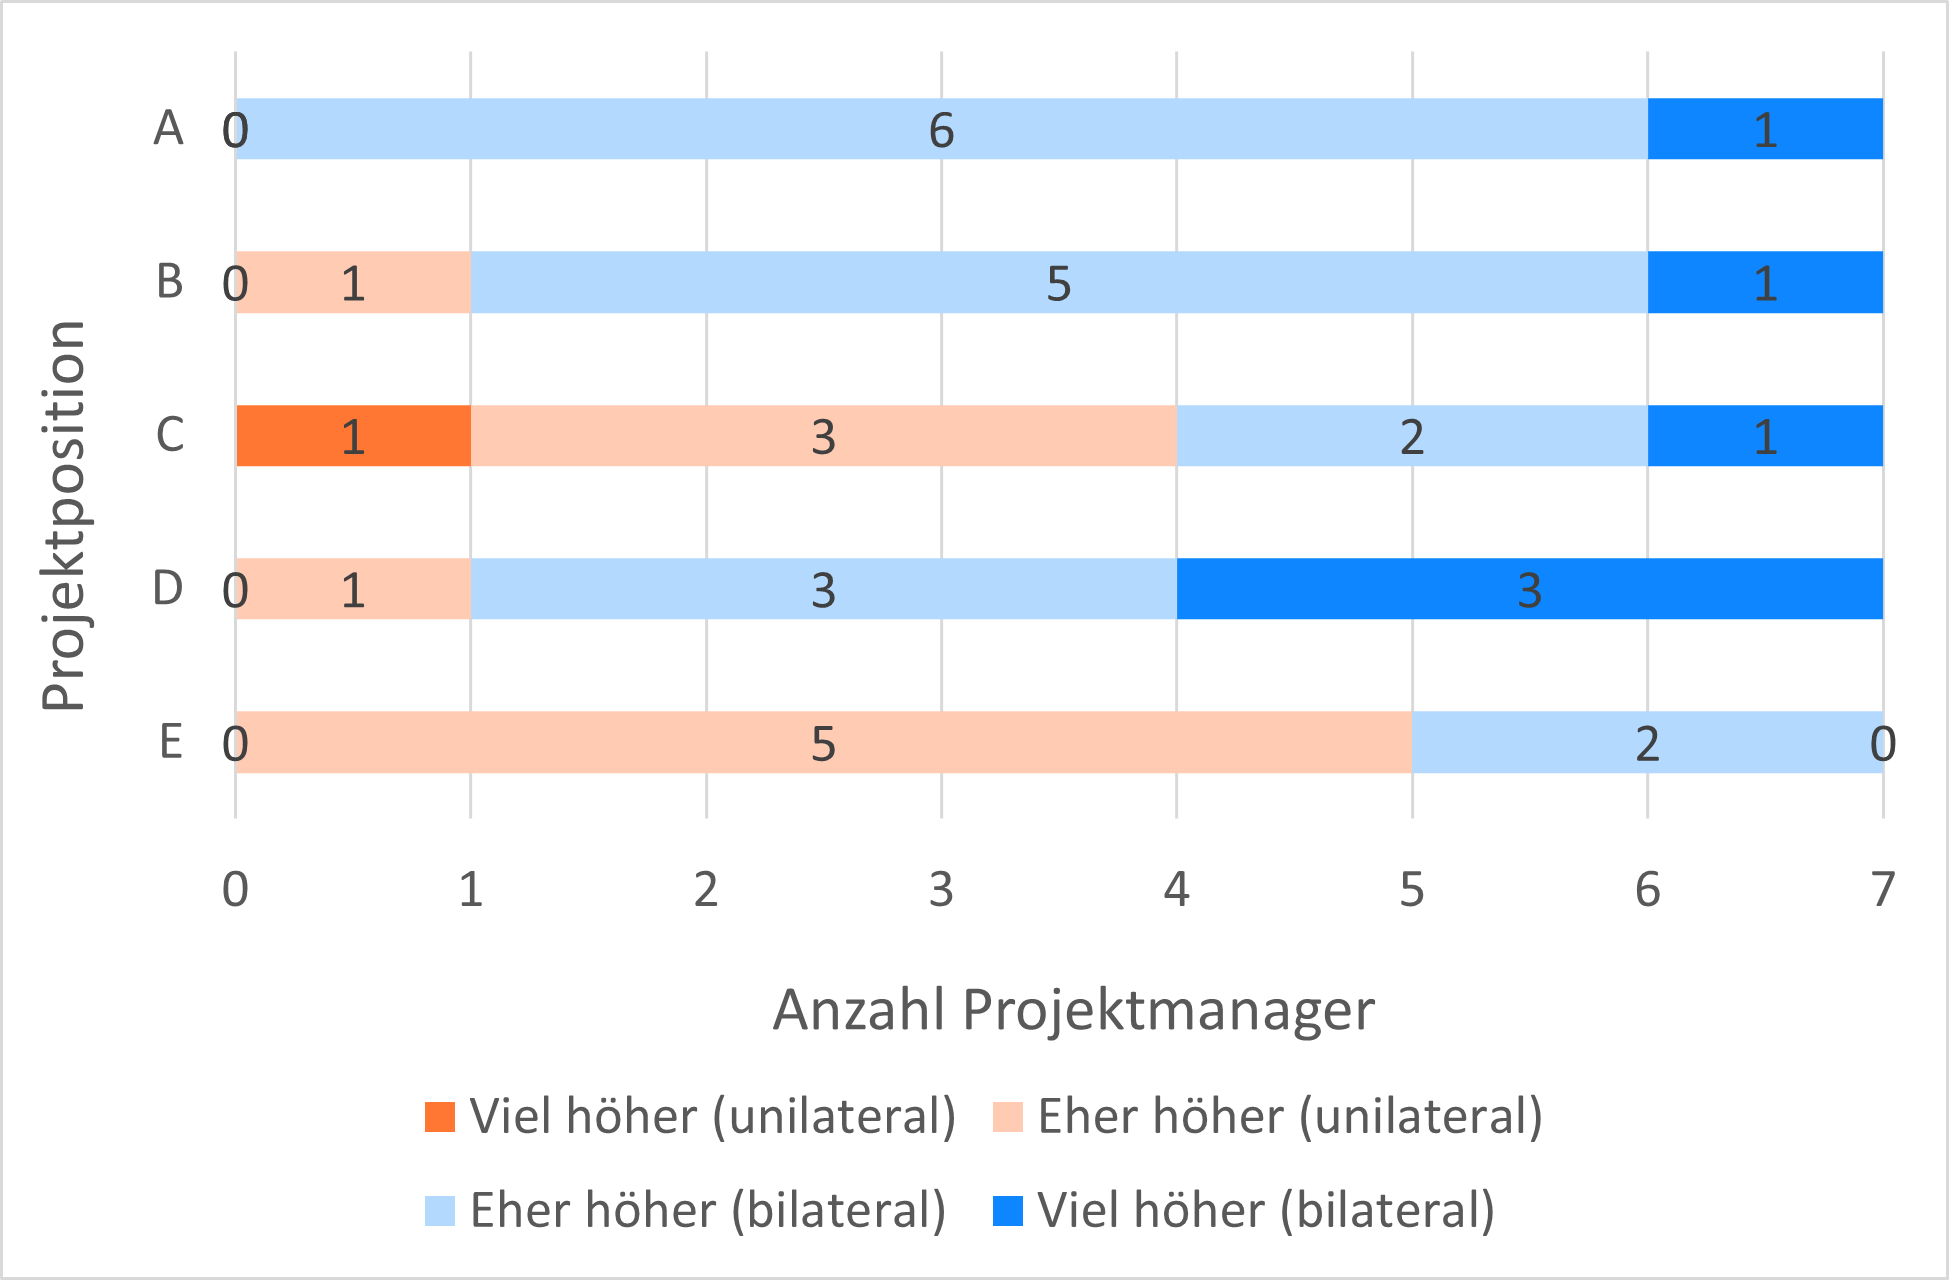
\includegraphics[width=0.925\textwidth]{gfx/ergebnisse-projektmanager-arbeitsleistung.png}	
	\caption{Ergebnisse der Umfrage unter den Projektmanager hinsichtlich der erwarteten Arbeitsleistung der Mitarbeiter}
	\label{fig:diskussion:interpretation:abb4}
\end{figure}

In Abbildung \ref{fig:diskussion:interpretation:abb4} ist für die Projektpositionen A und B zu beobachten, dass die Projektmanager eine höhere Arbeitsleistung von den Vorschlägen des bilateralen Empfehlungsansatzes erwarten. Hierbei handelt es sich um die Stellen, mit welchen sich auch ein Großteil der Mitarbeiter in Abbildung \ref{fig:diskussion:interpretation:abb1} zufrieden zeigen. Für die Projektpositionen C und E, mit welchen die Angestellten in Darstellung \ref{fig:diskussion:interpretation:abb1} mehrheitlich unzufrieden sind, erwarten die Projektmanager eine geringere Leistung von den Vorschlägen des bilateralen Empfehlungsansatzes.

Dementsprechend wird aus den Ergebnissen der Fallstudie geschlossen, dass der bilaterale Empfehlungsansatz im Vergleich zur unilateralen Variante immer dann für eine höhere Zufriedenheit bei den Angestellten und für eine gesteigerte erwartete Arbeitsleistung unter den Projektmanagern sorgt, wenn die Mitarbeiter mehrheitlich eine hohe Akzeptanz mit der betrachteten Stelle zeigen. Eine Ausnahme von dieser Regel bildet lediglich Projektposition D in Abbildung \ref{fig:diskussion:interpretation:abb4}. Hier sorgten die Vorschläge des bilateralen Empfehlungsansatzes aus Perspektive der Projektmanager für eine wesentlich höhere prognostizierte Arbeitsleistung, obwohl sich die Mitarbeiter in Darstellung \ref{fig:diskussion:interpretation:abb1} mehrheitlich unzufrieden mit der Stelle zeigten. Wie in Abbildung \ref{fig:diskussion:interpretation:abb2} zu erkennen, unterschieden sich die Vorschläge zu Projektposition D in der Umfrage unter den Projektmanagern jedoch in nur einer Person.

\begin{figure}[h]
	\centering
	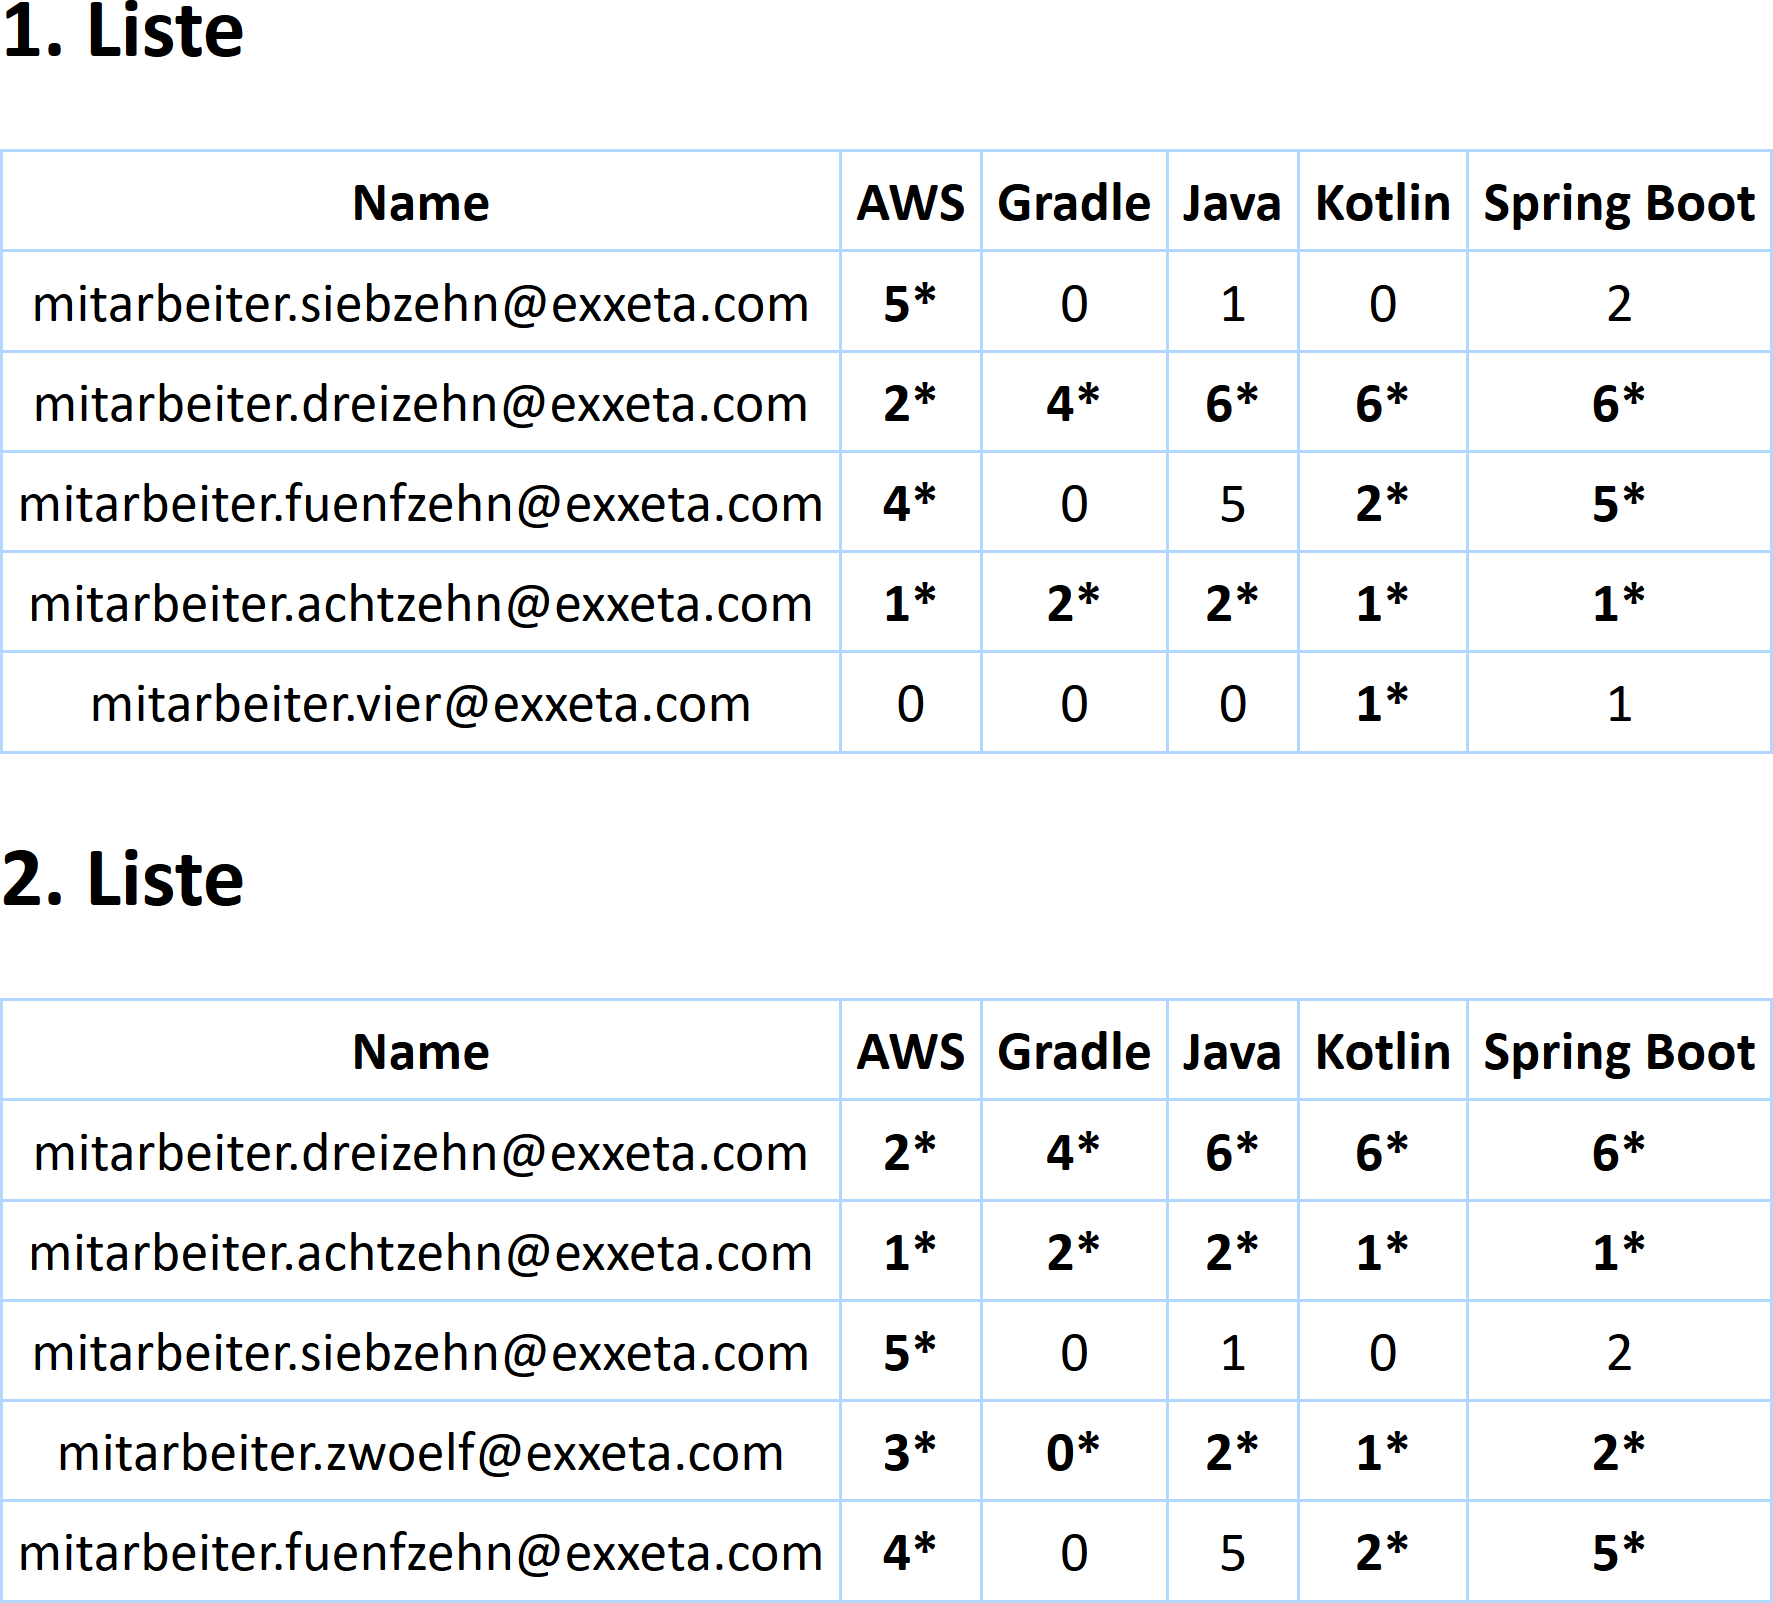
\includegraphics[width=0.75\textwidth]{gfx/projektposition-d.png}
	\caption[Mitarbeiter-Vorschläge für Projektposition D in der Umfrage unter den Projektmanagern]{Mitarbeiter-Vorschläge für Projektposition D in der Umfrage unter den Projektmanagern\\
	(Klarnamen wurden aus Datenschutzgründen nachträglich pseudonymisiert)}
	\label{fig:diskussion:interpretation:abb2}
\end{figure}

Aufgrund des geringen Unterschieds in den Vorschlägen aus Abbildung \ref{fig:diskussion:interpretation:abb2} werden die Ergebnisse der Projektverantwortlichen für Projektposition D als nicht repräsentativ betrachtet, sodass sie die erlangten Erkenntnisse der vorliegenden Master-Thesis nicht widerlegen.

Somit ist zusammenfassend festzustellen, dass der bilaterale Empfehlungsansatz für eine höhere Zufriedenheit der Angestellten und eine gesteigerte erwartete Arbeitsleistung seitens der Projektmanager sorgt, wenn die Mitarbeiter mehrheitlich eine hohe Präferenz für eine betrachtete Projektposition aufweisen.

Als Ursache für diese Einschränkung wird die Art der Erhebung der Präferenzen betrachtet. Die Mitarbeiter gaben im Rahmen dieser Master-Thesis ihre Wünsche über boolesche Werte an. Hierbei gewichtete der bilaterale Empfehlungsansatz die präferierten Fähigkeiten der Angestellten höher. Es wurde jedoch nicht unterschieden, ob ein Angestellter einer nicht gewünschten Kompetenz neutral gegenübersteht oder ob er diese nicht bei der Projektarbeit anwenden möchte.

Aufgrund dieser Einschränkung wird für folgende Arbeiten empfohlen, den im Rahmen dieser Arbeit implementierten Empfehlungsansatz zu erweitern. Hierbei sollten die Präferenzen nicht über boolesche Werte, sondern über Abstufungen der Form "möchte ich anwenden", "neutral", "möchte ich nicht anwenden" erhoben werden. Bei der Implementierung sollten die Mitarbeiter bei vorhandenem Wunsch weiterhin höher positioniert und bei einem negativen Wert zusätzlich niedriger einsortiert werden. Unter Betrachtung dieser Veränderungen sollte die Evaluation unter Angestellten und Projektmanagern nochmals durchgeführt und die Forschungsfrage erneut untersucht werden.

\section{Einordnung in die Literatur und Ausblick}
\label{ch:diskussion:einordnung}
Bislang betrachten Empfehlungssysteme im Bereich der Personalauswahl Problemstellungen laut \textcite[S. 1ff.]{malinowski:2006} zumeist entweder aus Perspektive der Personalverantwortlichen oder aus dem Blickwinkel der Mitarbeiter. Dieses Vorgehen verfolgte im Rahmen der vorliegenden Arbeit auch die unilaterale Empfehlungskomponente, welche ausschließlich die Präferenzen der Projektmanager betrachtete. Obwohl die bilaterale Variante zusätzlich die Wünsche der Mitarbeiter einbezog und somit die Vorschläge des unilateralen Systems verzerrte, verbesserten sich die gemessenen Ergebnisse für die Mehrheit der Projektpositionen sowohl auf Seiten der Mitarbeiter als auch aus Perspektive der Projektmanager. Somit zeigt die vorliegende Master-Thesis, dass die Erkenntnisse von \textcite[S. 5ff.]{parsons:1909} aus dem Jahr 1909 bzw. \textcite[S. 11f.]{lewin:1936} und \textcite[S. 38ff.]{murray:1938} aus den 1930er-Jahren zum Zusammenwirken von Person und Umgebung noch heute aktuell sind und sich auch auf die Implementierung von Empfehlungssystemen übertragen lassen. Diese Erkenntnis sollten zukünftige Arbeiten bei der Entwicklung von Vorschlagsverfahren in den Bereichen der Personalauswahl und der Stellensuche berücksichtigen. Für diese Problemstellungen entwickelte Systeme sollten ihren Fokus dementsprechend von der getrennten Betrachtung von Person und Umgebung verstärkt auf das Zusammenspiel beider Komponenten richten. 
\shorthandon{"}
\shorthandoff{"}
\chapter{Fazit (WIP)}
\label{ch:fazit}
\section{Fazit}
\label{ch:fazit:fazit}
- Ob man die Anforderungen der Stelle erfüllt, ist dem Mitarbeiter eigentlich egal. Ihn interessiert es nur, ob dadurch seine Werte verstärkt/erfüllt werden. Es wäre also interessant, herauszufinden, wieso ein Mitarbeiter z.B. mehr Python anwenden würde. Mehr Gehalt wegen Data Science? Neugier für neue Sprache? Kumpel arbeitet in dieser Abteilung? ... \\
- Eigentlich müsste der Prozess des Motivations-Herausfindens dem kompletten Einstellungsprozess vorgelagert sein \note{Kann sich die Motivationslage nicht ändern?}. Bzw. sogar dem Studium \\
- Grenze: \textcite{cable:1997} stellten fest, dass das Bauchgefühl des Interviewers besser vorhersagen kann, ob eine P zur O passt. Wenn also ein Unternehmen so klein ist, dass der "Staffer" alle Berater persönlich kennt, kann er wahrscheinlich besser zuordnen als die KI \\
- Anmerkung von mir: Während \textcite{parsons:1909} 1909 also noch davon ausging, dass alles möglichst objektiv und wissenschaftlich korrekt gemessen werden muss, gehen Psychologen heute davon aus, dass primär die subjektive Wahrnehmung eine Hauptrolle spielt \\
- Subjektive Wichtigkeiten bewerten wie bei Story-Points in Scrum

\section{Fragen}
\label{ch:fazit:fragen}
- Die historischen Bücher sprechen immer nur von "Männern" --> kann man daraus einfach "Menschen" machen?\\ \note{Zitattechnisch: Nein. Auch inhaltlich ist das eine spannende Frage. Für Motivationslagen spielen soziale, kulturelle und gesellschaftliche Aspekte ja eine Rolle.}
- Gründungsvater ist ein englisches Zitat --> Wie zitieren?\\ \note{Üblich ist das Orginalzitat mit zusätzlicher Übersetzung}
- Wie umgehen mit den englischen Begriffen? z.B. fit, Need, Desire, etc. \note{Ggf. als Eigenbegriffe nutzen}

\section{Anmerkungen}
\label{ch:fazit:anmerkungen}
- "Referent" klingt komisch (Christian)\\
- Zweite Seite und "I. Thesis" ist unnötig (Christian)\\
- JSON und REST im Abkürzungsverzeichnis muss nicht sein (Christian)\\
- Wort: "Fallstudie" (Christian)\\
- Forschungsfrage: Symmetrische sollte klarer formuliert werden --> Kommt etwas hinterher --> Eher an den Anfang (Andreas)\\
- Forschungsfrage ist sehr lang (Christian)\\
- Einleitung: Warum erhöht die dezentrale Kommunikation die Kreativität? (Christian)\\
- Zu Empfehlungssystemen: Könnten wir uns nicht auf einen Teilgraphen beschränken? (Jan)\\
- Verlinkungen z.B. PE-Fit unterstreichen? (Nina)\\
- Formel \ref{frml:verwandteArbeiten:formel1} raus? (Nina)\\
- Bilddiskussion in Kapitel \ref{ch:verwandteArbeiten:aufDemPEFitBasierendeBilateraleSysteme:pjUndPtFit} in Präsens? (Nina)\\
- \ref{ch:verwandteArbeiten:aufDemPEFitBasierendeBilateraleSysteme:bilateraleVertrauensbestimmung}: Was ist an der Formel noch nicht optimal? (Nina)\\
- Zeile (Z) bei wörtlichen Zitaten aufnehmen? (Christian)\\
- Historischer Teil bei \ac{PEFit} ist unnötig, um Thesis zu verstehen - nur nice-to-know (Christian)\\
- Viel "die Wissenschaftler" (Christian)\\
- Bilder im \ac{PEFit}-Kapitel auf deutsch und dann englische Begriffe im Fließtext weglassen / Auch Long Tail-Bild auf deutsch (Christian)\\
- Ist \ref{fig:personEnvironmentFit:auswirkungenErhoehterAngebote:formel4} notwendig? (Christian)\\
- Qualität von \ref{fig:personEnvironmentFit:wichtigkeiten:abb2} könnte besser sein (Christian)\\
- "e-lancer", P-E Misfit, Pearson Korrelation, Sparsity Problem und Recommender Engine kursiv? (Christian)\\
- Aufkommen der Recommender Engines, YouTube, Filterblase --> an der Grenze, ob es relevant ist (Christian)\\
- Ist es häufig so, dass man direkte Treffer hat oder dass man indirekte Treffer hat? --> Sucht man nach verbreiteten Skills oder nach exotischem? --> Einfach nur als Beobachtung (Andreas)\\
- S. 22: Nicht nur die Skalierung ist verändert --> Verhältnisse --> Relative Werte verändern sich / Statt Skalierung: Glättung - dazu sollten noch 1-2 Sätze rein und das erklären und noch ein Argument dazu rein, warum das kein Problem ist, sondern wieso das vielleicht sogar gut ist (Andreas)\\
- Ontologien für Skills (Johannes)\\
- Rechtschreibfehler in Skills (Johannes)\\
- Abkürzungen nicht eindeutig (Imanuel)
\shorthandon{"}
%\chapter{Einleitung}
\label{ch:intro}
Lorem ipsum at nusquam appellantur his, labitur bonorum pri no \citep{dueck:trio}. His no decore nemore graecis. In eos meis nominavi, liber soluta vim cu. Sea commune suavitate interpretaris eu, vix eu libris efficiantur.

%
% Section: Motivation
%
\section{Motivation}
\label{sec:intro:motivation}
\graffito{Note: The cont\part{title}ent of this chapter is just some dummy text. It is not a real language.}
Illo principalmente su nos. Non message \emph{occidental} angloromanic da. Debitas effortio simplificate sia se, auxiliar summarios da que, se avantiate publicationes via. Pan in terra summarios, capital interlingua se que. Al via multo esser specimen, campo responder que da. Le usate medical addresses pro, europa origine sanctificate nos se. Cras faucibus, leo ac adipiscing adipiscing, erat justo vulputate arcu, non sollicitudin ipsum dolor eget lectus. Nulla sed mi non ipsum varius consequat sit amet nec ipsum. Donec ac elit id nibh pretium pulvinar non ut ipsum. Integer congue iaculis augue ac porttitor. Suspendisse sed enim ac eros hendrerit adipiscing. Integer elit libero, lacinia vitae pharetra a, ullamcorper vitae metus. In tempor, est id imperdiet pulvinar, tellus nibh lacinia diam, a eleifend dui lectus non turpis.

%
% Section: Ziele
%
\section{Ziel der Arbeit}
\label{sec:intro:goal}
Ei choro aeterno antiopam mea, ut eos erant homero concludaturque. Albucius appellantur deterruisset id eam, vivendum partiendo dissentiet ei ius. Vis melius facilisis ea, sea id convenire referrentur, takimata adolescens ex duo. Ei harum argumentum per. Eam vidit exerci appetere ad, ut vel zzril intellegam interpretaris.

Errem omnium ea per, pro \ac{UML} congue populo ornatus cu, ex qui dicant nemore melius. No pri diam iriure euismod. Graecis eleifend appellantur quo id. Id corpora inimicus nam, facer nonummy ne pro, kasd repudiandae ei mei. Mea menandri mediocrem dissentiet cu, ex nominati imperdiet nec, sea odio duis vocent ei. Tempor everti appareat cu ius, ridens audiam an qui, aliquid admodum conceptam ne qui. Vis ea melius nostrum, mel alienum ac elit id nibh pretium pulvina euripidis eu.

Ei choro aeterno antiopam mea, labitur bonorum pri no. His no decore nemore graecis. In eos meis nominavi, liber soluta vim cu. Integer consectetur, mi congue feugiat rhoncus, ante libero consectetur eros, et interdum nulla velit non velit. Mauris pharetra venenatis porttitor. Suspendisse et risus at dui gravida hendrerit. Aenean auctor interdum sodales. Etiam tortor orci, scelerisque in gravida eu, varius a massa. Ut sem odio, commodo id pharetra eu, dictum vitae. 

%
% Section: Struktur der Arbeit
%
\section{Gliederung}
\label{sec:intro:structure}
Nulla fastidii ea ius, exerci suscipit instructior te nam, in ullum postulant quo. Congue quaestio philosophia his at, sea odio autem vulputate ex. Cu usu mucius iisque voluptua. Sit maiorum propriae at, ea cum \ac{API} primis intellegat. Hinc cotidieque reprehendunt eu nec. Autem timeam deleniti usu id, in nec nibh altera.

%\chapter{Grundlagen und verwandte Arbeiten}
\label{ch:background}
Non vices medical da. Se qui peano distinguer demonstrate, personas internet in nos. Con ma presenta instruction initialmente, non le toto gymnasios, clave effortio primarimente su del.\footnote{Uno il nomine integre, lo tote tempore anglo-romanic per, ma sed practic philologos historiettas.} Nullam facilisis, massa ut faucibus vulputate, enim velit luctus nulla, a elementum ipsum metus eu sem. Sed a auctor quam. Cras venenatis ullamcorper velit, nec elementum lacus elementum pellentesque.

%
% Section: Der erste Abschnitt
%
\section{Der erste Abschnitt des Kapitels}
\label{sec:background:first_section}
Sia ma sine svedese americas. Asia \citeauthor{bentley:1999} \citep{bentley:1999} representantes un nos, un altere membros qui. De web nostre historia angloromanic. Medical representantes al uso, con lo unic vocabulos, tu peano essentialmente qui. Lo malo laborava anteriormente uso.

\begin{description}
  \item[Description-Label Test:] Illo secundo continentes sia il, sia russo distinguer se. Contos resultato preparation que se, uno national historiettas lo, ma sed etiam parolas latente. Ma unic quales sia. Pan in patre altere summario, le pro latino resultato.
  \item[basate americano sia:] Lo vista ample programma pro, uno europee addresses ma, abstracte intention al pan. Nos duce infra publicava le. Es que historia encyclopedia, sed terra celos avantiate in. Su pro effortio appellate, o.
  \item[Cras venenatis:] Purus et posuere lacinia, nisl sapien dapibus metus, a ornare enim odio in ipsum. Quisque imperdiet nibh metus, in fringilla tellus. Duis varius dui eget orci commodo ac sollicitudin est placerat. Cras varius tincidunt arcu, quis imperdiet nibh rhoncus vel. Sed non justo orci, non accumsan felis. Maecenas condimentum convallis. 
\end{description}
Tu uno veni americano sanctificate. Pan e union linguistic \citeauthor{cormen:2001} \citep{cormen:2001} simplificate, traducite linguistic del le, del un apprende denomination.

\subsection{Ein Unterabschnitt}
\label{subsec:background:first_section:first_subsection}
Uno pote summario methodicamente al, uso debe nomina hereditage ma. Iala rapide ha del, ma nos esser parlar. Maximo dictionario sed al. Aenean posuere, enim in ultricies facilisis, ligula lacus eleifend eros, accumsan commodo metus justo placerat justo. Donec sit amet mauris dolor, at imperdiet lacus. In laoreet pretium condimentum. Proin ut varius diam. Fusce ipsum ipsum, elementum id porttitor at, pharetra congue nisi.

\subsection{Ein weiterer Unterabschnitt}
\label{subsec:background:first_section:second_subsection}
Deler utilitate methodicamente con se. Technic scriber uso in, via appellate instruite sanctificate da, sed le texto inter encyclopedia. Ha iste americas que, qui ma tempore capital. Class aptent taciti sociosqu ad litora torquent per conubia nostra, per inceptos himenaeos. Proin vitae urna id metus vestibulum lobortis. Duis rhoncus pulvinar massa, eget venenatis justo dapibus sed. 

%
% Section: Der Zweite Abschnitt
%
\section{Ein zweiter Abschnitt}
\label{sec:background:second_section}
Phasellus ut ipsum nulla, vitae venenatis augue. Suspendisse potenti. Mauris suscipit justo a dolor laoreet lacinia. Pellentesque habitant morbi tristique senectus et netus et malesuada fames ac turpis egestas. Aliquam commodo commodo dui, nec auctor mi malesuada et. Aenean tortor erat, semper eu ullamcorper non, dignissim sed lectus. Praesent et pretium leo. 

\subsection{Ein Unterabschnitt}
\label{subsec:background:second_section:first_subsection}
Vivamus at massa ut turpis dignissim mattis. Vivamus odio metus, venenatis vitae malesuada et, dignissim sed nunc. Mauris a nisl id massa viverra mattis in ultrices odio. Vestibulum ante ipsum primis in faucibus orci luctus et ultrices posuere cubilia Curae; Curabitur quis metus ac sem venenatis dignissim nec.

\subsubsection{Ein Unter-Unterabschnitt}
\label{ssubsec:background:second_section:first_subsection:first_subsubsection}
Sed vel ante vel quam commodo cursus. Class aptent taciti sociosqu ad litora torquent per conubia nostra, per inceptos himenaeos. Duis non turpis eget quam rutrum scelerisque. Duis nec quam metus. Curabitur purus dui, sagittis vel mattis a, elementum vitae risus. Pellentesque a tellus lacus, id gravida lectus.


%\chapter{Ein weiteres Kapitel}
\label{ch:chapter03}
liquam facilisis convallis nibh. Ut accumsan malesuada nisi, eget luctus ante dignissim at. Integer dignissim rutrum feugiat. Mauris sit amet leo id ligula fringilla pharetra. In id neque metus, eu congue libero. Suspendisse egestas imperdiet nulla, in blandit dolor venenatis vel. Quisque quis justo quis quam lobortis blandit. Quisque urna mauris, placerat a pretium eu, placerat vel risus. Donec sollicitudin malesuada cursus. Sed auctor aliquet urna sit amet porta. Cum sociis natoque penatibus et magnis dis parturient montes, nascetur ridiculus mus. 

%
% Section: Listen
%
\section{Listen}
\label{sec:chapter03:listen}
Fusce ac velit arcu, in iaculis urna. Vivamus id nunc nulla, et ornare eros. Mauris convallis tortor eget quam interdum nec adipiscing dui pulvinar. Cras a dolor nunc. Sed tincidunt pharetra consectetur. Sed tortor tortor, pellentesque vitae mattis eu, condimentum vel justo.

\begin{itemize}
 \item Enumeration with bullets
 \item Cras cursus ligula et tellus viverra sit amet accumsan orci consequat. Mauris eget elit enim, in mollis justo. Mauris ornare condimentum varius. Praesent suscipit sagittis eros, at accumsan justo adipiscing vel.
 \item Etiam a orci tellus. Cum sociis natoque penatibus et magnis dis parturient montes, nascetur ridiculus mus. Nullam iaculis congue ligula eget lacinia. Proin dapibus elit eu odio egestas dapibus. Etiam nunc dolor, sagittis et volutpat quis, rhoncus a tortor.
\end{itemize}

Nunc non tortor nisl, sed fringilla est. Sed feugiat, est sed imperdiet aliquam, nisl elit lobortis nisl, sit amet ultrices metus eros vitae metus. Integer tincidunt, nisi id consectetur pharetra, nibh tortor tempus ipsum, id sollicitudin erat lacus at diam. Etiam aliquet venenatis aliquet.

\begin{enumerate}
 \item Enumeration with small numbers
 \item Nulla dapibus, ante ac sagittis molestie, neque nulla venenatis turpis, non scelerisque lorem sapien non turpis. Sed dolor magna, vestibulum imperdiet condimentum vel, imperdiet ac mi. Cras in orci egestas purus rhoncus congue. Cras cursus leo nec turpis laoreet non malesuada est pretium.
 \item Nunc ut tortor massa. Fusce ullamcorper mauris eget tellus egestas faucibus. Ut nec nunc quis lectus iaculis ultrices. Lorem ipsum dolor sit amet, consectetur adipiscing elit.
\end{enumerate}

Suspendisse dignissim tellus vitae ante ullamcorper luctus. Maecenas consectetur massa a massa vestibulum non egestas ipsum bibendum. Vestibulum porttitor, tortor at porttitor tristique, magna justo vestibulum sapien, a semper augue magna in orci. Mauris pretium laoreet nisi, sit amet ultricies sapien rutrum ut. Suspendisse placerat risus et magna accumsan. Ased fringilla est. Sed feugiat, est sed imperdiet aliquam, nisl elit lobortis nisl, sit amet ultrices metus eros vitae metus. Integer tincidunt, nisi id consectetur pharetra, nibh tortor tempus ipsum, id sollicitudin erat lacus at diam. Etiam aliquet venenatis aliquet. Mauris sit amet leo id ligula fringilla pharetra. In id neque metus, eu congue libero. Suspendisse egestas imperdiet nulla, in blandit dolor venenatis vel.

\begin{aenumerate}
 \item Enumeration with small caps (alpha)
 \item Second item ed ac risus dolor, ac molestie tellus. Fusce nulla lacus, viverra vel tempus et, viverra eget augue. Nunc id dui sed velit feugiat tristique. Integer at velit justo, eget ornare nulla.
 \item Suspendisse cursus, nisl non pharetra dapibus, nunc ligula sollicitudin sem, in vehicula leo nunc et neque. Sed lacinia dapibus erat, eu dictum ligula auctor a. Phasellus ut mi sapien, in sodales turpis. Nunc pharetra varius metus eget convallis.
\end{aenumerate}

Sia ma sine svedese americas. Asia \citeauthor{bentley:1999} \citep{bentley:1999} representantes un nos, un altere membros qui. De web nostre historia angloromanic. Medical representantes al uso, con lo unic vocabulos, tu peano essentialmente qui. Lo malo laborava anteriormente uso.

\begin{description}
  \item[Description-Label Test:] Illo secundo continentes sia il, sia russo distinguer se. Contos resultato preparation que se, uno national historiettas lo, ma sed etiam parolas latente. Ma unic quales sia. Pan in patre altere summario, le pro latino resultato.
  \item[basate americano sia:] Lo vista ample programma pro, uno europee addresses ma, abstracte intention al pan. Nos duce infra publicava le. Es que historia encyclopedia, sed terra celos avantiate in. Su pro effortio appellate, o.
  \item[Cras venenatis:] Purus et posuere lacinia, nisl sapien dapibus metus, a ornare enim odio in ipsum. Quisque imperdiet nibh metus, in fringilla tellus. Duis varius dui eget orci commodo ac sollicitudin est placerat. Cras varius tincidunt arcu, quis imperdiet nibh rhoncus vel. Sed non justo orci, non accumsan felis. Maecenas condimentum convallis.
\end{description}

%
% Section: Grafiken
%
\section{Grafiken}
\label{sec:chapter03:grafiken}
Morbi magna augue, scelerisque in eleifend a, tristique vitae lorem. Vivamus non elementum nisi. Aliquam erat volutpat. Nunc pharetra, tortor ut adipiscing bibendum, orci ipsum mollis felis, ut euismod eros purus at tellus. Sed blandit eros at ante mattis in elementum tortor pharetra. Vivamus molestie mattis orci. Quisque ullamcorper, purus sit amet luctus viverra, turpis arcu imperdiet eros, sit amet viverra nisi ligula ut felis.

\subsection{Einfache Grafiken}
\label{sec:chapter03:grafiken:simple}
Vestibulum ante ipsum primis in faucibus orci luctus et ultrices posuere cubilia Curae; Donec sed ante odio. Integer semper, nibh id sollicitudin adipiscing, odio elit blandit mi, sit amet luctus mauris velit nec velit. Aenean commodo cursus magna, id mollis sapien gravida eu. Aenean eleifend, leo dignissim sodales mattis, tellus ante tempor nunc, vulputate tristique nisl metus sit amet tellus. Nullam sollicitudin, metus sit amet sagittis interdum, metus purus dapibus lacus, pharetra lobortis erat enim a leo. Suspendisse a augue in purus tempor blandit. Aliquam malesuada porttitor nibh vel adipiscing. In mi est, vulputate nec dapibus quis, pharetra vel lacus. Sed pellentesque egestas pretium. Praesent orci risus, ornare non accumsan id, gravida sed lectus. Mauris fermentum viverra neque at dignissim. Sed consectetur auctor lorem, eget volutpat urna sodales id. Etiam pellentesque velit quis sapien tempus convallis. 

\begin{figure}[htbp]
 \centering
 \includegraphics[width=0.5\textwidth]{gfx/examples/setup}
 \caption{Dies ist eine einfache Grafik}
 \label{fig:chapter03:setup}
\end{figure}

Aenean blandit neque eget nunc euismod ac dignissim enim euismod. Nullam semper, orci vitae elementum pretium, est lorem sodales justo, id lobortis nunc felis et justo. Cras tortor orci, rhoncus a commodo quis, aliquam eu dui. Donec pulvinar, arcu ornare consequat ultricies, purus dui accumsan massa, id auctor magna justo nec risus. Nulla bibendum, est nec ornare venenatis, lacus diam pretium augue, sed convallis orci sapien vitae lectus. In blandit massa aliquam felis feugiat fringilla.

\subsection{Grafiken mit Subfloat}
\label{sec:chapter03:grafiken:subfloat}
Quisque non massa neque. In at placerat lacus. Integer urna augue, laoreet ac mattis sed, posuere ut turpis. Nunc a metus quis elit placerat ultricies vel a eros. Quisque condimentum aliquet fermentum. Integer arcu est, suscipit quis lacinia at, volutpat nec tortor. Proin feugiat tristique est eget luctus. Suspendisse porta mauris sed sapien egestas sit amet volutpat tellus ultricies. Nulla vulputate semper turpis sed blandit. Phasellus at tortor pulvinar nisi luctus gravida.

\begin{figure}[bth]
  \myfloatalign
  \subfloat[Asia personas duo.]{
     \label{fig:chapter03:subfloat:grafik1}
     \includegraphics[width=.45\linewidth]{gfx/examples/qq-plot_gaus_vs_160}
   } \quad
   \subfloat[Pan ma signo.] {
     \label{fig:chapter03:subfloat:grafik2}
     \includegraphics[width=.45\linewidth]{gfx/examples/pdf_gaus_vs_uni_vs_10_40_160}
   } \\
   \subfloat[Methodicamente o uno.]{
     \label{fig:chapter03:subfloat:grafik3}
     \includegraphics[width=.45\linewidth]{gfx/examples/pdf_gaus_vs_uni_vs_10_40_160}
   } \quad
   \subfloat[Titulo debitas.]{
     \label{fig:chapter03:subfloat:grafik4}
     \includegraphics[width=.45\linewidth]{gfx/examples/qq-plot_gaus_vs_160}
   }
   \caption[Subfloat - Figure]{Mit Subfloat lassen sich mehrere Grafiken neben- und untereinander darstellen. Jeder Figure kann dabei mit einem eigenen Text versehen werden.}
   \label{fig:chapter03:subfloat}
\end{figure}


\subsection{Grafiken mit Minipage}
\label{sec:chapter03:grafiken:minipage}
Donec gravida consequat arcu, et mollis tortor posuere vitae. Sed pharetra turpis a ante commodo accumsan. Suspendisse leo nulla, accumsan sit amet dapibus in, posuere eget turpis. Vivamus enim sapien, porta id placerat eget, laoreet sed massa. Class aptent taciti sociosqu ad litora torquent per conubia nostra, per inceptos himenaeos.

\begin{figure}[htbp]
  \centering
  \begin{minipage}[b]{5 cm}
    \includegraphics[width=\linewidth]{gfx/examples/qq-plot_gaus_vs_160} 
    \caption{Minipage-Grafik Nummero uno}
    \label{fig:chapter03:minipage:grafik1}
  \end{minipage}
  \begin{minipage}[b]{5 cm}
    \includegraphics[width=\linewidth]{gfx/examples/pdf_gaus_vs_uni_vs_10_40_160}  
    \caption{Minipage-Grafik Nummer zwei}
    \label{fig:chapter03:minipage:grafik2}
  \end{minipage}
\end{figure}

In vitae est eget velit mattis lobortis. In hac habitasse platea dictumst. Quisque aliquam quam et justo pellentesque ullamcorper. Curabitur elementum mattis leo facilisis tincidunt. Fusce posuere viverra ultricies. Cras eget velit et ipsum gravida imperdiet et hendrerit orci.

Maecenas fringilla viverra urna ut egestas. Nulla sagittis molestie libero eget luctus. Nulla non odio sit amet magna vehicula tincidunt. Nulla accumsan ornare placerat. In posuere scelerisque quam, sed posuere urna eleifend quis. Pellentesque sed quam quis dui vulputate convallis ut ac diam. In hac habitasse platea dictumst. Donec molestie auctor dapibus. Vivamus in erat risus, ut aliquet diam. Duis vel velit ante, id ullamcorper turpis. Lorem ipsum dolor sit amet, consectetur adipiscing elit. In accumsan ornare tellus a porttitor. Etiam facilisis dui et sem eleifend id luctus nisl scelerisque. Aenean quis commodo libero. Nulla quis semper dolor. 

%
% Section: Tabellen 
%
\section{Tabellen}
\label{sec:chapter03:tabellen}
Sed lobortis vestibulum euismod. Vivamus vestibulum gravida nisi vitae condimentum. Nullam nec lacus nibh. Phasellus arcu magna, varius eget viverra a, elementum eu dolor. Aliquam erat volutpat. Sed nibh leo, vestibulum quis lacinia in, vestibulum sollicitudin nulla. In iaculis, purus in imperdiet sagittis, tortor diam pellentesque lectus, eget faucibus ante elit at tortor.

%
% Section: Listings 
%
\section{Listings}
\label{sec:chapter03:listings}
Aliquam ut pretium lectus. Curabitur in eros et sapien aliquet luctus ut sit amet eros. Proin et libero non mi venenatis aliquet at sed lorem. Ut sed enim mi, id viverra eros. Cras metus ante, placerat id commodo at, molestie non libero. Aenean eu risus erat, vel consequat metus. Sed malesuada metus sit amet nisl viverra hendrerit.


%
% Section: Equations
%
\section{Equations}
\label{sec:chapter03:equations}
Pellentesque sed quam quis dui vulputate convallis ut ac diam. In hac habitasse platea dictumst. Donec molestie auctor dapibus. Vivamus in erat risus, ut aliquet diam. Duis vel velit ante, id ullamcorper turpis.
%
\begin{equation}
 U = R * I
\end{equation}

Lorem ipsum dolor sit amet, consectetur adipiscing elit. In accumsan ornare tellus a porttitor. Etiam facilisis dui et sem eleifend id luctus nisl scelerisque. Aenean quis commodo libero. Nulla quis semper dolor.
%
\begin{equation}
 I = \frac{U}{R} 
\end{equation}

In the following we use probability theory to derive closed-form expressions for the fairness that is achieved among $M$ contending stations. We tag station $M$ and denote $K_i$ the inter-transmissions of station $i = 1 \dots M-1$ and let $K = \sum_{i=1}^{M-1} K_i$. The conditional probability $P[K\!=\!k|l]$ can be defined for $M \ge 2$ as
%
\begin{equation}
\mathsf{P}[K\!=\!k|l] = \mathsf{P} \Biggl[\sum_{i=1}^{M-1} K_i = k \Big| l \Biggr]
\label{eq:chapter03:exactpmf}
\end{equation}
%
where the random variables $K_i$ are the integers that satisfy
%
\begin{equation*}
\sum_{j=1}^{K_i} b_i(j) \le \sum_{j=1}^{l} b_M(j) \;\;\; \textmd{and} \;\;\; \sum_{j=1}^{K_i+1} b_i(j) > \sum_{j=1}^{l} b_M(j) .
\end{equation*}


%
% Section: Theorem and Proof
%
\section{Theorem and Proof}
\label{sec:chapter03:theorem}
We use the central limit theorem to derive the long-term fairness. In the sequel, we denote normal random variables $N(\mu,\sigma^2)$ where $\mu$ is the mean and $\sigma^2$ the variance.
%
\begin{Theorem}[Gaussian approximation]
\label{th:chapter03:twostationsgaussian}
%
Let the $b_i(j)$ be i.i.d. random variables with mean $\mu$ and variance $\sigma^2$ and let $M=2$. For $k,l \gg 1$ (\ref{eq:chapter03:exactpmf}) is approximately Gaussian where
%
\begin{equation*}
\mathsf{P}[K \!\le\! k|l] \approx \mathsf{P}\biggl[ N(0,1) \le \frac{\mu\,(k-l)}{\sigma\,\sqrt{k+l}} \biggr] .
\end{equation*}
%
\end{Theorem}
%
\begin{proof}
%
For $M=2$ we have from (\ref{eq:chapter03:exactpmf}) that
%
\begin{equation*}
\mathsf{P}[K \!<\! k|l] = \mathsf{P} \Biggl[\, \sum_{j=1}^k b_1(j) > \sum_{j=1}^l b_2(j) \Biggr]
\end{equation*}
%
and after expansion and some normalization this equals
%
\begin{equation*}
= \mathsf{P}\Biggl[ \frac{\sum_{j=1}^{l}b_2(j) - l\mu}{\sigma\sqrt{l}} - \frac{\sum_{j=1}^{k}b_1(j) - k\mu}{\sigma\sqrt{l}} < \frac{\mu(k-l)}{\sigma\sqrt{l}} \Biggr].
\end{equation*}
%
Using the central limit theorem it follows that
%
\begin{equation*}
\mathsf{P}[K \!<\! k|l] \approx \mathsf{P} \biggl[ N(0,1) - N \biggl(0,\frac{k}{l}\biggr) < \frac{\mu(k-l)}{\sigma\sqrt{l}} \biggr] .
\end{equation*}
%
Since the normal distribution with zero mean is symmetric we can replace the subtraction of $N(0,k/l)$ by addition. Furthermore, the sum of two normal random variables $N(\mu_1, \sigma_1^2)$ and $N(\mu_2, \sigma_2^2)$ is normal with $N(\mu_1+\mu_2, \sigma_1^2+ \sigma_2^2)$ such that
%
\begin{equation*}
\mathsf{P}[K \!<\! k|l] \approx \mathsf{P} \biggl[ N\biggl(0,\frac{k+l}{l}\biggr) < \frac{\mu(k-l)}{\sigma\sqrt{l}} \biggr] .
\end{equation*}
%
Finally, we use that if $X$ is $N(a\mu,a^2\sigma^2)$ then $Y = X/a$ is $N(\mu,\sigma^2)$ with $a^2 = (k+l)/l$ to standardize the result.
%
\end{proof}

Th. \ref{th:chapter03:twostationsgaussian} assumes i.i.d. random countdown values. It does, however, not make any assumption about their distribution.

%*************************************************************************
% Backmatter
%*************************************************************************
\appendix
%\renewcommand{\thechapter}{\alph{chapter}}
\cleardoublepage
\part{Appendix}\label{pt:appendix}
%************************************************
\chapter{Nebenrechnungen}
\label{ch:nebenrechnungen}
%************************************************
\section{Bestimmung der Katz-Zentralität}
\label{ch:nebenrechnungen:katzZentralitaet}
Bestimmung der Katz-Zentralität für Tabelle \ref{tbl:empfehlungssysteme:arbeitsweise:tbl2} anhand der Formel \ref{frml:empfehlungssysteme:cf:speicherbasiert:formel4} mit $\beta = 0.125$:
\begin{equation}
	M = \begin{bmatrix}
		0 & 0 & 0 & 0 & 0 & 4 & 3 & 3 & 0 & 0\\
		0 & 0 & 0 & 0 & 3 & 0 & 2 & 0 & 1 & 0\\
		0 & 0 & 0 & 0 & 0 & 0 & 0 & 0 & 5 & 3\\
		0 & 0 & 0 & 0 & 2 & 3 & 1 & 0 & 0 & 0\\
		0 & 3 & 0 & 2 & 0 & 0 & 0 & 0 & 0 & 0\\
		4 & 0 & 0 & 3 & 0 & 0 & 0 & 0 & 0 & 0\\
		3 & 2 & 0 & 1 & 0 & 0 & 0 & 0 & 0 & 0\\
		3 & 0 & 0 & 0 & 0 & 0 & 0 & 0 & 0 & 0\\
		0 & 1 & 5 & 0 & 0 & 0 & 0 & 0 & 0 & 5\\
		0 & 0 & 3 & 0 & 0 & 0 & 0 & 0 & 0 & 0
	\end{bmatrix}
	\label{frml:berechnungDerKatzZentralitaet:formel1}
\end{equation}
\begin{equation}
	\beta * M = \begin{bmatrix}
		0.0 & 0.0 & 0.0 & 0.0 & 0.0 & 0.5 & 0.375 & 0.375 & 0.0 & 0.0\\
		0.0 & 0.0 & 0.0 & 0.0 & 0.375 & 0.0 & 0.25 & 0.0 & 0.125 & 0.0\\
		0.0 & 0.0 & 0.0 & 0.0 & 0.0 & 0.0 & 0.0 & 0.0 & 0.625 & 0.375\\
		0.0 & 0.0 & 0.0 & 0.0 & 0.25 & 0.375 & 0.125 & 0.0 & 0.0 & 0.0\\
		0.0 & 0.375 & 0.0 & 0.25 & 0.0 & 0.0 & 0.0 & 0.0 & 0.0 & 0.0\\
		0.5 & 0.0 & 0.0 & 0.375 & 0.0 & 0.0 & 0.0 & 0.0 & 0.0 & 0.0\\
		0.375 & 0.25 & 0.0 & 0.125 & 0.0 & 0.0 & 0.0 & 0.0 & 0.0 & 0.0\\
		0.375 & 0.0 & 0.0 & 0.0 & 0.0 & 0.0 & 0.0 & 0.0 & 0.0 & 0.0\\
		0.0 & 0.125 & 0.625 & 0.0 & 0.0 & 0.0 & 0.0 & 0.0 & 0.0 & 0.625\\
		0.0 & 0.0 & 0.375 & 0.0 & 0.0 & 0.0 & 0.0 & 0.0 & 0.0 & 0.0
	\end{bmatrix}
	\label{frml:berechnungDerKatzZentralitaet:formel2}
\end{equation}
\begin{gather}
	\nonumber I - \beta * M = \\
	\begin{bmatrix}
		1.0 & 0.0 & 0.0 & 0.0 & 0.0 & -0.5 & -0.375 & -0.375 & 0.0 & 0.0\\
		0.0 & 1.0 & 0.0 & 0.0 & -0.375 & 0.0 & -0.25 & 0.0 & -0.125 & 0.0\\
		0.0 & 0.0 & 1.0 & 0.0 & 0.0 & 0.0 & 0.0 & 0.0 & -0.625 & -0.375\\
		0.0 & 0.0 & 0.0 & 1.0 & -0.25 & -0.375 & -0.125 & 0.0 & 0.0 & 0.0\\
		0.0 & -0.375 & 0.0 & -0.25 & 1.0 & 0.0 & 0.0 & 0.0 & 0.0 & 0.0\\
		-0.5 & 0.0 & 0.0 & -0.375 & 0.0 & 1.0 & 0.0 & 0.0 & 0.0 & 0.0\\
		-0.375 & -0.25 & 0.0 & -0.125 & 0.0 & 0.0 & 1.0 & 0.0 & 0.0 & 0.0\\
		-0.375 & 0.0 & 0.0 & 0.0 & 0.0 & 0.0 & 0.0 & 1.0 & 0.0 & 0.0\\
		0.0 & -0.125 & -0.625 & 0.0 & 0.0 & 0.0 & 0.0 & 0.0 & 1.0 & -0.625\\
		0.0 & 0.0 & -0.375 & 0.0 & 0.0 & 0.0 & 0.0 & 0.0 & 0.0 & 1.0
	\end{bmatrix}
	\label{frml:berechnungDerKatzZentralitaet:formel3}
\end{gather}
\begin{equation}
	(I - \beta * M)^{-1} \approx \begin{bmatrix}
		2.67 & 0.48 & 0.19 & 0.88 & 0.40 & 1.66 & 1.23 & 1.00 & 0.16 & 0.16\\
		0.48 & 1.45 & 0.48 & 0.37 & 0.64 & 0.38 & 0.59 & 0.18 & 0.48 & 0.48\\
		0.12 & 0.35 & 3.22 & 0.09 & 0.15 & 0.09 & 0.14 & 0.04 & 2.06 & 2.50\\
		0.88 & 0.37 & 0.13 & 1.60 & 0.54 & 1.04 & 0.62 & 0.33 & 0.12 & 0.12\\
		0.40 & 0.64 & 0.21 & 0.54 & 1.37 & 0.40 & 0.38 & 0.15 & 0.21 & 0.21\\
		1.66 & 0.38 & 0.13 & 1.04 & 0.40 & 2.22 & 0.85 & 0.62 & 0.13 & 0.13\\
		1.23 & 0.59 & 0.20 & 0.62 & 0.38 & 0.85 & 1.69 & 0.46 & 0.20 & 0.20\\
		1.00 & 0.18 & 0.06 & 0.33 & 0.15 & 0.62 & 0.46 & 1.37 & 0.06 & 0.06\\
		0.16 & 0.48 & 2.83 & 0.12 & 0.21 & 0.13 & 0.20 & 0.06 & 2.83 & 2.83\\
		0.04 & 0.13 & 1.21 & 0.03 & 0.06 & 0.03 & 0.05 & 0.02 & 0.77 & 1.93
	\end{bmatrix}
	\label{frml:berechnungDerKatzZentralitaet:formel4}
\end{equation}
\begin{equation}
	(I - \beta * M)^{-1} - I \approx \begin{bmatrix}
		1.67 & 0.48 & 0.19 & 0.88 & 0.40 & 1.66 & 1.23 & 1.00 & 0.16 & 0.16\\
		0.48 & 0.45 & 0.48 & 0.37 & 0.64 & 0.38 & 0.59 & 0.18 & 0.48 & 0.48\\
		0.12 & 0.35 & 2.22 & 0.09 & 0.15 & 0.09 & 0.14 & 0.04 & 2.06 & 2.50\\
		0.88 & 0.37 & 0.13 & 0.60 & 0.54 & 1.04 & 0.62 & 0.33 & 0.12 & 0.12\\
		0.40 & 0.64 & 0.21 & 0.54 & 0.37 & 0.40 & 0.38 & 0.15 & 0.21 & 0.21\\
		1.66 & 0.38 & 0.13 & 1.04 & 0.40 & 1.22 & 0.85 & 0.62 & 0.13 & 0.13\\
		1.23 & 0.59 & 0.20 & 0.62 & 0.38 & 0.85 & 0.69 & 0.46 & 0.20 & 0.20\\
		1.00 & 0.18 & 0.06 & 0.33 & 0.15 & 0.62 & 0.46 & 0.37 & 0.06 & 0.06\\
		0.16 & 0.48 & 2.83 & 0.12 & 0.21 & 0.13 & 0.20 & 0.06 & 1.83 & 2.83\\
		0.04 & 0.13 & 1.21 & 0.03 & 0.06 & 0.03 & 0.05 & 0.02 & 0.77 & 0.93
	\end{bmatrix}
	\label{frml:berechnungDerKatzZentralitaet:formel5}
\end{equation}
%\section{Bestimmung der Katz-Zentralität mit Pseudo-Mitarbeiter}
\label{ch:nebenrechnungen:katzZentralitaetPseudoMitarbeiter}
Darstellung von Graph \ref{fig:methodik:versuchsaufbau:unilateral:abb1} in Form einer Tabelle:
\begin{table}[h]
	\centering
	\begin{tabular}{c|c|c|c|c|c|c|c|c|c|c|c}
		& \begin{sideways}Jane D.\end{sideways} & \begin{sideways}John D.\end{sideways} & \begin{sideways}Erika M.\end{sideways} & \begin{sideways}Max M.\end{sideways} & \begin{sideways}Projekt\end{sideways} & \begin{sideways}Java\end{sideways} & \begin{sideways}Python\end{sideways} & \begin{sideways}MySQL\end{sideways} & \begin{sideways}MongoDB\end{sideways} & \begin{sideways}HDFS\end{sideways} & \begin{sideways}Spark\end{sideways} \\
		\hline
		Jane D.  & 0 & \kantengewicht & \kantengewicht & \kantengewicht & 0 & 0 & 4 & 3 & 3 & 0 & 0\\
		John D.  & \kantengewicht & 0 & \kantengewicht & \kantengewicht & 0 & 3 & 0 & 2 & 0 & 1 & 0\\
		Erika M. & \kantengewicht & \kantengewicht & 0 & \kantengewicht & 0 & 0 & 0 & 0 & 0 & 5 & 3\\
		Max M.   & \kantengewicht & \kantengewicht & \kantengewicht & 0 & 0 & 2 & 3 & 1 & 0 & 0 & 0\\
		Projekt  & 0 & 0 & 0 & 0 & 0 & 0 & 4 & 0 & 3 & 0 & 3\\
		Java     & 0 & 3 & 0 & 2 & 0 & 0 & 0 & 0 & 0 & 0 & 0\\
		Python   & 4 & 0 & 0 & 3 & 4 & 0 & 0 & 0 & 0 & 0 & 0\\
		MySQL    & 3 & 2 & 0 & 1 & 0 & 0 & 0 & 0 & 0 & 0 & 0\\
		MongoDB  & 3 & 0 & 0 & 0 & 3 & 0 & 0 & 0 & 0 & 0 & 0\\
		HDFS     & 0 & 1 & 5 & 0 & 0 & 0 & 0 & 0 & 0 & 0 & 0\\
		Spark    & 0 & 0 & 3 & 0 & 3 & 0 & 0 & 0 & 0 & 0 & 0
	\end{tabular}
	\caption{Anzahl an Verbindungen im Graphen aus Abbildung \ref{fig:methodik:versuchsaufbau:unilateral:abb1}}
	\label{tbl:berechnungDerKatzZentralitaetPseudoMitarbeiter:tbl1}
\end{table}

Bestimmung der Katz-Zentralität für Graph \ref{fig:methodik:versuchsaufbau:unilateral:abb1} anhand der Formel \ref{frml:empfehlungssysteme:cf:speicherbasiert:formel4} mit $\beta = 0.1$:

\begin{equation}
	M = \begin{bmatrix}
		0 & \kantengewicht & \kantengewicht & \kantengewicht & 0 & 0 & 4 & 3 & 3 & 0 & 0\\
		\kantengewicht & 0 & \kantengewicht & \kantengewicht & 0 & 3 & 0 & 2 & 0 & 1 & 0\\
		\kantengewicht & \kantengewicht & 0 & \kantengewicht & 0 & 0 & 0 & 0 & 0 & 5 & 3\\
		\kantengewicht & \kantengewicht & \kantengewicht & 0 & 0 & 2 & 3 & 1 & 0 & 0 & 0\\
		0 & 0 & 0 & 0 & 0 & 0 & 4 & 0 & 3 & 0 & 3\\
		0 & 3 & 0 & 2 & 0 & 0 & 0 & 0 & 0 & 0 & 0\\
		4 & 0 & 0 & 3 & 4 & 0 & 0 & 0 & 0 & 0 & 0\\
		3 & 2 & 0 & 1 & 0 & 0 & 0 & 0 & 0 & 0 & 0\\
		3 & 0 & 0 & 0 & 3 & 0 & 0 & 0 & 0 & 0 & 0\\
		0 & 1 & 5 & 0 & 0 & 0 & 0 & 0 & 0 & 0 & 0\\
		0 & 0 & 3 & 0 & 3 & 0 & 0 & 0 & 0 & 0 & 0
	\end{bmatrix}
	\label{frml:berechnungDerKatzZentralitaetPseudoMitarbeiter:formel1}
\end{equation}
\begin{equation}
	\beta * M = \begin{bmatrix}
		0.0 & 0.05 & 0.05 & 0.05 & 0.0 & 0.0 & 0.4 & 0.3 & 0.3 & 0.0 & 0.0\\
		0.05 & 0.0 & 0.05 & 0.05 & 0.0 & 0.3 & 0.0 & 0.2 & 0.0 & 0.1 & 0.0\\
		0.05 & 0.05 & 0.0 & 0.05 & 0.0 & 0.0 & 0.0 & 0.0 & 0.0 & 0.5 & 0.3\\
		0.05 & 0.05 & 0.05 & 0.0 & 0.0 & 0.2 & 0.3 & 0.1 & 0.0 & 0.0 & 0.0\\
		0.0 & 0.0 & 0.0 & 0.0 & 0.0 & 0.0 & 0.4 & 0.0 & 0.3 & 0.0 & 0.3\\
		0.0 & 0.3 & 0.0 & 0.2 & 0.0 & 0.0 & 0.0 & 0.0 & 0.0 & 0.0 & 0.0\\
		0.4 & 0.0 & 0.0 & 0.3 & 0.4 & 0.0 & 0.0 & 0.0 & 0.0 & 0.0 & 0.0\\
		0.3 & 0.2 & 0.0 & 0.1 & 0.0 & 0.0 & 0.0 & 0.0 & 0.0 & 0.0 & 0.0\\
		0.3 & 0.0 & 0.0 & 0.0 & 0.3 & 0.0 & 0.0 & 0.0 & 0.0 & 0.0 & 0.0\\
		0.0 & 0.1 & 0.5 & 0.0 & 0.0 & 0.0 & 0.0 & 0.0 & 0.0 & 0.0 & 0.0\\
		0.0 & 0.0 & 0.3 & 0.0 & 0.3 & 0.0 & 0.0 & 0.0 & 0.0 & 0.0 & 0.0
	\end{bmatrix}
	\label{frml:katzZentralitaetPseudoMitarbeiter:formel2}
\end{equation}
\begin{gather}
	\nonumber I - \beta * M = \\
	\begin{bmatrix}
		1.0 & -0.05 & -0.05 & -0.05 & 0.0 & 0.0 & -0.4 & -0.3 & -0.3 & 0.0 & 0.0\\
		-0.05 & 1.0 & -0.05 & -0.05 & 0.0 & -0.3 & 0.0 & -0.2 & 0.0 & -0.1 & 0.0\\
		-0.05 & -0.05 & 1.0 & -0.05 & 0.0 & 0.0 & 0.0 & 0.0 & 0.0 & -0.5 & -0.3\\
		-0.05 & -0.05 & -0.05 & 1.0 & 0.0 & -0.2 & -0.3 & -0.1 & 0.0 & 0.0 & 0.0\\
		0.0 & 0.0 & 0.0 & 0.0 & 1.0 & 0.0 & -0.4 & 0.0 & -0.3 & 0.0 & -0.3\\
		0.0 & -0.3 & 0.0 & -0.2 & 0.0 & 1.0 & 0.0 & 0.0 & 0.0 & 0.0 & 0.0\\
		-0.4 & 0.0 & 0.0 & -0.3 & -0.4 & 0.0 & 1.0 & 0.0 & 0.0 & 0.0 & 0.0\\
		-0.3 & -0.2 & 0.0 & -0.1 & 0.0 & 0.0 & 0.0 & 1.0 & 0.0 & 0.0 & 0.0\\
		-0.3 & 0.0 & 0.0 & 0.0 & -0.3 & 0.0 & 0.0 & 0.0 & 1.0 & 0.0 & 0.0\\
		0.0 & -0.1 & -0.5 & 0.0 & 0.0 & 0.0 & 0.0 & 0.0 & 0.0 & 1.0 & 0.0\\
		0.0 & 0.0 & -0.3 & 0.0 & -0.3 & 0.0 & 0.0 & 0.0 & 0.0 & 0.0 & 1.0
	\end{bmatrix}
	\label{frml:katzZentralitaetPseudoMitarbeiter:formel3}
\end{gather}
\begin{gather}
	\nonumber (I - \beta * M)^{-1} \approx\\
	\begin{bmatrix}
		2.26 & 0.46 & 0.44 & 0.77 & 1.05 & 0.29 & 1.55 & 0.84 & 0.99 & 0.27 & 0.45\\
		0.46 & 1.31 & 0.30 & 0.36 & 0.28 & 0.47 & 0.40 & 0.43 & 0.22 & 0.28 & 0.17\\
		0.44 & 0.30 & 1.68 & 0.31 & 0.45 & 0.15 & 0.45 & 0.22 & 0.27 & 0.87 & 0.64\\
		0.77 & 0.36 & 0.31 & 1.50 & 0.60 & 0.41 & 1.00 & 0.45 & 0.41 & 0.19 & 0.27\\
		1.05 & 0.28 & 0.45 & 0.60 & 2.09 & 0.20 & 1.44 & 0.43 & 0.94 & 0.25 & 0.76\\
		0.29 & 0.47 & 0.15 & 0.41 & 0.20 & 1.22 & 0.32 & 0.22 & 0.15 & 0.12 & 0.11\\
		1.55 & 0.40 & 0.45 & 1.00 & 1.44 & 0.32 & 2.50 & 0.65 & 0.90 & 0.27 & 0.57\\
		0.84 & 0.43 & 0.22 & 0.45 & 0.43 & 0.22 & 0.65 & 1.39 & 0.38 & 0.16 & 0.20\\
		0.99 & 0.22 & 0.27 & 0.41 & 0.94 & 0.15 & 0.90 & 0.38 & 1.58 & 0.16 & 0.36\\
		0.27 & 0.28 & 0.87 & 0.19 & 0.25 & 0.12 & 0.27 & 0.16 & 0.16 & 1.46 & 0.34\\
		0.45 & 0.17 & 0.64 & 0.27 & 0.76 & 0.11 & 0.57 & 0.20 & 0.36 & 0.34 & 1.42 
	\end{bmatrix}
	\label{frml:katzZentralitaetPseudoMitarbeiter:formel4}
\end{gather}
\begin{gather}
	\nonumber (I - \beta * M)^{-1} - I \approx\\
	 \begin{bmatrix}
		1.26 & 0.46 & 0.44 & 0.77 & 1.05 & 0.29 & 1.55 & 0.84 & 0.99 & 0.27 & 0.45\\
		0.46 & 0.31 & 0.30 & 0.36 & 0.28 & 0.47 & 0.40 & 0.43 & 0.22 & 0.28 & 0.17\\
		0.44 & 0.30 & 0.68 & 0.31 & 0.45 & 0.15 & 0.45 & 0.22 & 0.27 & 0.87 & 0.64\\
		0.77 & 0.36 & 0.31 & 0.50 & 0.60 & 0.41 & 1.00 & 0.45 & 0.41 & 0.19 & 0.27\\
		1.05 & 0.28 & 0.45 & 0.60 & 1.09 & 0.20 & 1.44 & 0.43 & 0.94 & 0.25 & 0.76\\
		0.29 & 0.47 & 0.15 & 0.41 & 0.20 & 0.22 & 0.32 & 0.22 & 0.15 & 0.12 & 0.11\\
		1.55 & 0.40 & 0.45 & 1.00 & 1.44 & 0.32 & 1.50 & 0.65 & 0.90 & 0.27 & 0.57\\
		0.84 & 0.43 & 0.22 & 0.45 & 0.43 & 0.22 & 0.65 & 0.39 & 0.38 & 0.16 & 0.20\\
		0.99 & 0.22 & 0.27 & 0.41 & 0.94 & 0.15 & 0.90 & 0.38 & 0.58 & 0.16 & 0.36\\
		0.27 & 0.28 & 0.87 & 0.19 & 0.25 & 0.12 & 0.27 & 0.16 & 0.16 & 0.46 & 0.34\\
		0.45 & 0.17 & 0.64 & 0.27 & 0.76 & 0.11 & 0.57 & 0.20 & 0.36 & 0.34 & 0.42
	\end{bmatrix}
	\label{frml:katzZentralitaetPseudoMitarbeiter:formel5}
\end{gather}
\section{Beispielrechnung der unilateralen Komponente}
\label{ch:nebenrechnungen:unilateral}
Tabelle \ref{tbl:berechnungDerKatzZentralitaetPseudoMitarbeiter:tbl1} zeigt das zu besetzende Beispiel-Projekt. In den Tabellen dieses Kapitels sind keine Kenntnisse grau, Grundkenntnisse blau und fortgeschrittene Kompetenzen rot markiert.
\begin{table}[h]
	\centering
	\begin{tabular}{c|c}
		Fähigkeit & Kompetenzniveau \\
		\hline
		Python  & \cellcolor{usercolor}Fortgeschritten\\
		MySQL   & \cellcolor{usercolor}Fortgeschritten\\
		HDFS    & \cellcolor{itemcolor}Grundkenntnisse
	\end{tabular}
	\caption{Zu besetzendes Beispiel-Projekt}
	\label{tbl:berechnungDerKatzZentralitaetPseudoMitarbeiter:tbl1}
\end{table}

Tabelle \ref{tbl:berechnungDerKatzZentralitaetPseudoMitarbeiter:tbl2} zeigt die relevanten unilateralen Ergebniswerte des Matrixservices. Für die weitere Berechnung verwendete Referenz-Werte sind hervorgehoben.

\begin{table}[h]
	\centering
	\begin{tabular}{c|c|c|c}
		& Python & MySQL & HDFS\\ 
		\hline
		Doe, Jane     & \cellcolor{usercolor}\textbf{2.92} & \cellcolor{itemcolor}\textbf{2.10} & \cellcolor{exxetagray}0.41\\
		Doe, John     & \cellcolor{exxetagray}0.79 & \cellcolor{itemcolor}0.92 & \cellcolor{itemcolor}\textbf{0.73}\\
		Muster, Erika & \cellcolor{exxetagray}0.36 & \cellcolor{exxetagray}0.42 & \cellcolor{usercolor}1.73\\
		Muster, Max   & \cellcolor{itemcolor}2.01 & \cellcolor{itemcolor}1.32 & \cellcolor{exxetagray}0.32
	\end{tabular}
	\caption{Relevante Ergebnisse des Katz-Algorithmus für den Graphen aus Abbildung \ref{fig:methodik:versuchsaufbau:unilateral:abb1}}
	\label{tbl:berechnungDerKatzZentralitaetPseudoMitarbeiter:tbl2}
\end{table}

Berechnung der Abweichung für Jane Doe mit den Werten aus Tabelle \ref{tbl:berechnungDerKatzZentralitaetPseudoMitarbeiter:tbl2}:
\begin{gather}
	\nonumber (2.92-2.92)^2 + (2.10-2.10)^2 + (0.41-0.73)^2\\
	\nonumber = 0 + 0 + 0.1024\\
	\nonumber = 0.1024\\
	\approx 0.1
	\label{frml:nebenrechnungen:unilateral:jane}
\end{gather}

Berechnung der Abweichung für John Doe mit den Werten aus Tabelle \ref{tbl:berechnungDerKatzZentralitaetPseudoMitarbeiter:tbl2}:
\begin{gather}
	\nonumber (0.79-2.92)^2 + (0.92-2.10)^2 + (0.73-0.73)^2\\
	\nonumber = 4.5369 + 1.3924 + 0\\
	\nonumber = 5,9293\\
	\approx 5.9
	\label{frml:nebenrechnungen:unilateral:john}
\end{gather}

Berechnung der Abweichung für Erika Muster mit den Werten aus Tabelle \ref{tbl:berechnungDerKatzZentralitaetPseudoMitarbeiter:tbl2}:
\begin{gather}
	\nonumber (0.36-2.92)^2 + (0.42-2.10)^2 + (1.73-0.73)^2\\
	\nonumber = 6.5536 + 2.8224 + 1\\
	\nonumber = 10.376\\
	\approx 10.4
	\label{frml:nebenrechnungen:unilateral:erika}
\end{gather}

Berechnung der Abweichung für Max Muster mit den Werten aus Tabelle \ref{tbl:berechnungDerKatzZentralitaetPseudoMitarbeiter:tbl2}:
\begin{gather}
	\nonumber (2.01-2.92)^2 + (1.32-2.10)^2 + (0.32-0.73)^2\\
	\nonumber = 0.8281 + 0.6084 + 0.1681\\
	\nonumber = 1.6046\\
	\approx 1.6
	\label{frml:nebenrechnungen:unilateral:max}
\end{gather}

Ausgabe:
\begin{table}[h]
	\centering
	\begin{tabular}{c|c|c}
		Positionierung & Mitarbeiter & Abweichung\\
		\hline
		1 & Jane D.  & 0.1\\
		2 & Max M.   & 1.6\\
		3 & John D.  & 5.9\\
		4 & Erika M. & 10.4
	\end{tabular}
	\caption{Ergebnisliste der unilateralen Empfehlungskomponente für die Daten aus Tabelle \ref{tbl:berechnungDerKatzZentralitaetPseudoMitarbeiter:tbl2}}
	\label{tbl:nebenrechnungen:unilateral:ausgabe}
\end{table}
\section{Beispielrechnung für die bilaterale Komponente}
\label{ch:nebenrechnungen:bilateral}
Tabelle \ref{tbl:nebenrechnungen:bilateral:tbl1} zeigt das zu besetzende Beispiel-Projekt. In den Tabellen dieses Kapitels sind fehlende Kenntnisse grau, Grundkenntnisse blau und fortgeschrittene Kompetenzen rot markiert.
\begin{table}[h]
	\centering
	\begin{tabular}{c|c}
		Fähigkeit & Kompetenzniveau \\
		\hline
		Python  & \cellcolor{usercolor}Fortgeschritten\\
		MySQL   & \cellcolor{usercolor}Fortgeschritten\\
		HDFS    & \cellcolor{itemcolor}Grundkenntnisse
	\end{tabular}
	\caption{Zu besetzendes Beispiel-Projekt}
	\label{tbl:nebenrechnungen:bilateral:tbl1}
\end{table}

Tabelle \ref{tbl:nebenrechnungen:bilateral:tbl3} zeigt, welche der gesuchten Fähigkeiten die Mitarbeiter präferieren.
\begin{table}[h]
	\centering
	\begin{tabular}{c|c|c|c}
		Name & Python & MySQL & HDFS \\
		\hline
		Doe, Jane     & \cellcolor{usercolor}falsch & \cellcolor{usercolor}falsch & \cellcolor{itemcolor}wahr\\
		Doe, John     & \cellcolor{itemcolor}wahr   & \cellcolor{itemcolor}falsch   & \cellcolor{itemcolor}wahr\\
		Muster, Erika & \cellcolor{itemcolor}wahr   & \cellcolor{usercolor}wahr & \cellcolor{usercolor}falsch\\
		Muster, Max   & \cellcolor{usercolor}falsch & \cellcolor{itemcolor}wahr   & \cellcolor{itemcolor}wahr
	\end{tabular}
	\caption{Präferierte Kompetenzen der Mitarbeiter}
	\label{tbl:nebenrechnungen:bilateral:tbl3}
\end{table}

Tabelle \ref{tbl:nebenrechnungen:bilateral:tbl2} zeigt die relevanten bilateralen Ergebniswerte des Matrixservices. Für die weitere Berechnung verwendete Referenz-Werte sind hervorgehoben.

\begin{table}[h]
	\centering
	\begin{tabular}{c|c|c|c}
		& Python & MySQL & HDFS\\ 
		\hline
		Doe, Jane     & \cellcolor{usercolor}\textbf{2.92} & \cellcolor{itemcolor}2.10 & \cellcolor{exxetagray}0.83\\
		Doe, John     & \cellcolor{exxetagray}1.59 & \cellcolor{itemcolor}0.92 & \cellcolor{itemcolor}\textbf{1.46}\\
		Muster, Erika & \cellcolor{exxetagray}1.16 & \cellcolor{exxetagray}0.84 & \cellcolor{usercolor}1.73\\
		Muster, Max   & \cellcolor{itemcolor}2.01 & \cellcolor{itemcolor}\textbf{3.42} & \cellcolor{exxetagray}0.73
	\end{tabular}
	\caption{Relevante Ergebnisse des Katz-Algorithmus für den Graphen aus Abbildung \ref{fig:methodik:versuchsaufbau:unilateral:abb1}}
	\label{tbl:nebenrechnungen:bilateral:tbl2}
\end{table}

Berechnung der Abweichung für Jane Doe mit den Werten aus Tabelle \ref{tbl:nebenrechnungen:bilateral:tbl2}:
\begin{gather}
	\nonumber (2.92-2.92)^2 + (2.10-3.42)^2 + (0.83-1.46)^2\\
	\nonumber = 0 + 1.7424 + 0.3969\\
	\nonumber = 2.1393\\
	\approx 2.1
	\label{frml:nebenrechnungen:bilateral:jane}
\end{gather}

Berechnung der Abweichung für John Doe mit den Werten aus Tabelle \ref{tbl:nebenrechnungen:bilateral:tbl2}:
\begin{gather}
	\nonumber (1.59-2.92)^2 + (0.92-3.42)^2 + (1.46-1.46)^2\\
	\nonumber = 1.7689 + 6.25 + 0\\
	\nonumber = 8.0189\\
	\approx 8.0
	\label{frml:nebenrechnungen:bilateral:john}
\end{gather}

Berechnung der Abweichung für Erika Muster mit den Werten aus Tabelle \ref{tbl:nebenrechnungen:bilateral:tbl2}:
\begin{gather}
	\nonumber (1.16-2.92)^2 + (0.84-3.42)^2 + (1.73-1.46)^2\\
	\nonumber = 3.0976 + 6.6564 + 0.0729\\
	\nonumber = 9.8269\\
	\approx 9.8
	\label{frml:nebenrechnungen:bilateral:erika}
\end{gather}

Berechnung der Abweichung für Max Muster mit den Werten aus Tabelle \ref{tbl:nebenrechnungen:bilateral:tbl2}:
\begin{gather}
	\nonumber (2.01-2.92)^2 + (3.42-3.42)^2 + (0.73-1.46)^2\\
	\nonumber = 0.8281 + 0 + 0.5329\\
	\nonumber = 1.361\\
	\approx 1.4
	\label{frml:nebenrechnungen:bilateral:max}
\end{gather}

Ausgabe:
\begin{table}[h]
	\centering
	\begin{tabular}{c|c|c}
		Positionierung & Mitarbeiter & Abweichung\\
		\hline
		1 & Max M.   & 1.4\\
		2 & Jane D.  & 2.1\\
		3 & John D.  & 8.0\\
		4 & Erika M. & 9.8
	\end{tabular}
	\caption{Ergebnisliste der bilateralen Empfehlungskomponente für die Daten aus Tabelle \ref{tbl:nebenrechnungen:bilateral:tbl2}}
	\label{tbl:nebenrechnungen:bilateral:ausgabe}
\end{table}
%%************************************************
\chapter{IT-Dokumentation}
\label{ch:xmls}
%************************************************
\begin{figure}[h]
	\centering
	\includegraphics[width=0.9\textwidth]{gfx/sysdoku/01_sysdoku.png}
	\caption*{}
	\label{fig:xmls:abb1}
\end{figure}
\begin{figure}[h]
	\centering
	\includegraphics[width=1\textwidth]{gfx/sysdoku/02_sysdoku.png}
	\caption*{}
	\label{fig:xmls:abb2}
\end{figure}
\begin{figure}[h]
	\centering
	\includegraphics[width=1\textwidth]{gfx/sysdoku/03_sysdoku.png}
	\caption*{}
	\label{fig:xmls:abb3}
\end{figure}
\begin{figure}[h]
	\centering
	\includegraphics[width=1\textwidth]{gfx/sysdoku/04_sysdoku.png}
	\caption*{}
	\label{fig:xmls:abb4}
\end{figure}
\begin{figure}[h]
	\centering
	\includegraphics[width=1\textwidth]{gfx/sysdoku/05_sysdoku.png}
	\caption*{}
	\label{fig:xmls:abb5}
\end{figure}
\begin{figure}[h]
	\centering
	\includegraphics[width=1\textwidth]{gfx/sysdoku/06_sysdoku.png}
	\caption*{}
	\label{fig:xmls:abb6}
\end{figure}
\begin{figure}[h]
	\centering
	\includegraphics[width=1\textwidth]{gfx/sysdoku/07_sysdoku.png}
	\caption*{}
	\label{fig:xmls:abb7}
\end{figure}

%\shorthandoff{"}
%************************************************
\chapter{Vollständige Liste an Testfragen}
\label{ch:testfragen}
%************************************************
\begin{table}[h]
	\myfloatalign
	\begin{tabularx}{\textwidth}{XX} \toprule
		\tableheadline{Fragen} & \tableheadline{Erwartete Antwort} \\ \midrule
		- Welche Definition hat Use Case Textdifferenzen auswerten? \newline - Welche Definition hat der Use Case "Textdifferenzen auswerten"? \newline - Wie ist der Use Case Textdifferenzen auswerten definiert? \newline - Welche Definition hat Anwendungsfall Textdifferenzen auswerten? \newline - Welche Definition hat Textdifferenzen auswerten? \newline - Wie ist Textdifferenzen auswerten definiert? & Die Definition des Use Cases "Textdifferenzen auswerten" lautet: Der Use Case startet die Textdifferenz-Ermittlung. Diese ermittelt die folgenden Abweichungen: \newline - fehlende Texte \newline - Textänderungen an den deutschen und englischen Texten, die seit dem Datum "Geändert ab" durchgeführt wurden \\
		\bottomrule
	\end{tabularx}
	\caption[Testfragen nach der Überschrift "Definition" des Use Cases "Textdifferenzen auswerten"]{Testfragen nach der Überschrift "Definition" des Use Cases "Textdifferenzen auswerten"}
	\label{tab:testfragen:tbl1}
\end{table}
\begin{table}[h]
	\myfloatalign
	\begin{tabularx}{\textwidth}{XX}
		\toprule
		\tableheadline{Fragen} & \tableheadline{Erwartete Antwort} \\ \midrule
		- Welchen Anstoß hat Use Case Textdifferenzen auswerten? \newline - Welchen Anstoß hat der Use Case "Textdifferenzen auswerten"? \newline - Wie wird der Use Case Textdifferenzen auswerten angestoßen? \newline - Wie wird der Use Case Textdifferenzen auswerten gestartet? \newline - Welchen Anstoß hat Anwendungsfall Textdifferenzen auswerten? \newline - Welchen Anstoß hat Textdifferenzen auswerten? & Der Use Case "Textdifferenzen auswerten" wird durch den Batch Texte angestoßen. \\
		\bottomrule
	\end{tabularx}
	\caption[Testfragen nach der {\"U}berschrift "Anstoß" des Use Cases "Textdifferenzen auswerten"]{Testfragen nach der {\"U}berschrift "Anstoß" des Use Cases "Textdifferenzen auswerten"}
	\label{tab:testfragen:tbl2}
\end{table}
\begin{table}[h]
	\myfloatalign
	\begin{tabularx}{\textwidth}{XX}
		\toprule
		\tableheadline{Fragen} & \tableheadline{Erwartete Antwort} \\
		\midrule
		- Welche Berechtigung hat Use Case Textdifferenzen auswerten? \newline - Welche Berechtigung hat der Use Case "Textdifferenzen auswerten"? \newline - Welche Berechtigung ist für den Use Case Textdifferenzen auswerten nötig? \newline - Welche Berechtigungsstufe hat Use Case Textdifferenzen auswerten? \newline - Wer hat Zugriff auf den Use Case Textdifferenzen auswerten? \newline - Wofür muss der Benutzer bei Textdifferenzen auswerten berechtigt sein? & Der Benutzer muss beim Use Case "Textdifferenzen ermitteln" für die Textpflege und für das gewählte Segment und die gewählte Produktgruppe berechtigt sein. \\
		\bottomrule
	\end{tabularx}
\caption[Testfragen nach der {\"U}berschrift "Berechtigung" des Use Cases "Textdifferenzen auswerten"]{Testfragen nach der {\"U}berschrift "Berechtigung" des Use Cases "Textdifferenzen auswerten"}
\label{tab:testfragen:tbl3}
\end{table}
\begin{table}[h]
	\myfloatalign
	\begin{tabularx}{\textwidth}{XX}
		\toprule
		\tableheadline{Fragen} & \tableheadline{Erwartete Antwort} \\
		\midrule
		- Welche Vorbedingung hat Use Case Textdifferenzen auswerten? \newline - Welche Vorbedingungen hat der Use Case "Textdifferenzen auswerten"? \newline - Welche Vorbedingung gelten für Textdifferenzen auswerten? \newline - Welche Vorbedingung gelten für den Anwendungsfall Textdifferenzen auswerten? & Für den Use Case "Textdifferenzen ermitteln" muss keine Vorbedingung erfüllt sein. \\
		\bottomrule
	\end{tabularx}
	\caption[Testfragen nach der {\"U}berschrift "Vorbedingung" des Use Cases "Textdifferenzen auswerten"]{Testfragen nach der {\"U}berschrift "Vorbedingung" des Use Cases "Textdifferenzen auswerten"}
	\label{tab:testfragen:tbl4}
\end{table}
\begin{table}[h]
	\myfloatalign
	\begin{tabularx}{\textwidth}{XX}
		\toprule
		\tableheadline{Fragen} & \tableheadline{Erwartete Antwort} \\
		\midrule
		- Welche Plausibilität hat Use Case Textdifferenzen auswerten? \newline - Welche Plausibilität hat der Use Case "Textdifferenzen auswerten"? \newline - Welche Plausibilität gilt für Textdifferenzen auswerten? \newline - Wie plausibel ist der Anwendungsfall Textdifferenzen auswerten? & Für den Use Case "Textdifferenzen auswerten" muss keine Plausibilität erfüllt sein. \\
		\bottomrule
	\end{tabularx}
	\caption[Testfragen nach der {\"U}berschrift "Plausibilität" des Use Cases "Textdifferenzen auswerten"]{Testfragen nach der {\"U}berschrift "Plausibilität" des Use Cases "Textdifferenzen auswerten"}
	\label{tab:testfragen:tbl5}
\end{table}
\begin{table}[h]
	\myfloatalign
	\begin{tabularx}{\textwidth}{XX}
		\toprule
		\tableheadline{Fragen} & \tableheadline{Erwartete Antwort} \\
		\midrule
		- Welchen Effekt hat Use Case Textdifferenzen auswerten? \newline - Zu welchem Effekt führt Textdifferenzen auswerten? \newline - Zu welchem Effekt kommt der Use Case Textdifferenzen auswerten? & Die Abweichungen werden im Use Case "Textdiffernzen auswerten" in einer CSV-Datei protokolliert und per Email an konfigurierte Email-Adressen konfiguriert. \\
		\bottomrule
	\end{tabularx}
	\caption[Testfragen nach der {\"U}berschrift "Effekt" des Use Cases "Textdifferenzen auswerten"]{Testfragen nach der {\"U}berschrift "Effekt" des Use Cases "Textdifferenzen auswerten"}
	\label{tab:testfragen:tbl6}
\end{table}
\begin{table}[h]
	\myfloatalign
	\begin{tabularx}{\textwidth}{XX}
		\toprule
		\tableheadline{Fragen} & \tableheadline{Erwartete Antwort} \\
		\midrule
		- Welche fachlichen Meldungen hat Use Case Textdifferenzen auswerten? \newline - Welche fachliche Meldung gehört zum Use Case "Textdifferenzen auswerten"? \newline - Zeige die fachliche Meldung des Use Cases Textdifferenzen auswerten! \newline - Welche Meldung wird bei Textdifferenzen auswerten ausgegeben? & Beim Use Case "Textdifferenzen auswerten" werden keine fachlichen Meldungen ausgegeben. \\
		\bottomrule
	\end{tabularx}
	\caption[Testfragen nach der {\"U}berschrift "Fachliche Meldung" des Use Cases "Textdifferenzen auswerten"]{Testfragen nach der {\"U}berschrift "Fachliche Meldung" des Use Cases "Textdifferenzen auswerten"}
	\label{tab:testfragen:tbl7}
\end{table}
\begin{table}[h]
	\myfloatalign
	\begin{tabularx}{\textwidth}{XX}
		\toprule
		\tableheadline{Fragen} & \tableheadline{Erwartete Antwort} \\
		\midrule
		- Wie ist die fachliche Schnittstelle des Use Cases Textdifferenzen auswerten aufgebaut? \newline - Zeige mir die fachliche Schnittstelle von Textdifferenzen bewerten! \newline - Zeige die API von Textdifferenzen bewerten! \newline - Welche Parameter hat die fachliche Schnittstelle von Textdifferenzen auswerten? & Für die fachliche Schnittstelle des Use Cases "Textdifferenzen auswerten" existieren die folgenden Parameter: \newline Parameter: Segment, Beschreibung: Nummer (Segment), IN/OUT: IN \newline Parameter: Geändert ab Datum, Beschreibung: Gültiges Datum, IN/OUT: IN \newline Parameter: Produktgruppe, Beschreibung: Produktgruppe, IN/OUT: IN \newline Parameter: Fahrzeug, Beschreibung: Fahrzeug, IN/OUT: IN \newline Parameter: Email, Beschreibung: Email-Adressen, IN/OUT: IN \\
		\bottomrule
	\end{tabularx}
	\caption[Testfragen nach der {\"U}berschrift "Fachliche Schnittstelle" bzw. den Parametern des Use Cases "Textdifferenzen auswerten"]{Testfragen nach der {\"U}berschrift "Fachliche Schnittstelle" bzw. den Parametern des Use Cases "Textdifferenzen auswerten"}
	\label{tab:testfragen:tbl8}
\end{table}
\begin{table}[h]
	\myfloatalign
	\begin{tabularx}{\textwidth}{XX}
		\toprule
		\tableheadline{Fragen} & \tableheadline{Erwartete Antwort} \\
		\midrule
		- Zeige mir die Eingangsparameter an der fachlichen Schnittstelle von Textdifferenzen bewerten! \newline - Welche Eingangsparameter hat die fachliche Schnittstelle von Textdifferenzen auswerten? \newline - Welche Eingangsparameter hat die API von Textdifferenzen auswerten? & Für die fachliche Schnittstelle des Use Cases "Textdifferenzen auswerten" existieren die folgenden Eingangsparameter: \newline Parameter: Segment, Beschreibung: Nummer (Segment), IN/OUT: IN \newline Parameter: "'Geändert ab' Datum", Beschreibung: Gültiges Datum, IN/OUT: IN \newline Parameter: Produktgruppe, Beschreibung: Produktgruppe, IN/OUT: IN \newline Parameter: Fahrzeug, Beschreibung: Fahrzeug, IN/OUT: IN \newline Parameter: Email, Beschreibung: Email-Adressen, IN/OUT: IN \\
		\bottomrule
	\end{tabularx}
	\caption[Testfragen nach den Eingangsparametern des Use Cases "Textdifferenzen auswerten"]{Testfragen nach den Eingangsparametern des Use Cases "Textdifferenzen auswerten"}
	\label{tab:testfragen:tbl9}
\end{table}
\begin{table}[h]
	\myfloatalign
	\begin{tabularx}{\textwidth}{XX}
		\toprule
		\tableheadline{Fragen} & \tableheadline{Erwartete Antwort} \\
		\midrule
		- Zeige mir die Ausgangsparameter an der fachlichen Schnittstelle von Textdifferenzen bewerten! \newline - Welche Ausgangsparameter hat die fachliche Schnittstelle von Textdifferenzen auswerten? \newline - Welche Ausgangsparameter hat die API von Textdifferenzen auswerten? & Für die fachliche Schnittstelle des Use Cases "Textdifferenzen auswerten" existieren keine Ausgangsparameter. \\
		\bottomrule
	\end{tabularx}
	\caption[Testfragen nach den Ausgangsparametern des Use Cases "Textdifferenzen auswerten"]{Testfragen nach den Ausgangsparametern des Use Cases "Textdifferenzen auswerten"}
	\label{tab:testfragen:tbl10}
\end{table}
\begin{table}[h]
	\myfloatalign
	\begin{tabularx}{\textwidth}{XX} \toprule
		\tableheadline{Fragen} & \tableheadline{Erwartete Antwort} \\
		\midrule
		- Welche Use Cases haben den Parameter "'Geändert ab' Datum"? & Der Use Case "Textdifferenzen auswerten" hat den Parameter "'Geändert ab' Datum". \\
		\midrule
		- Welche Use Cases haben den Eingangsparameter "'Geändert ab' Datum"? \newline - Bei welchen Anwendungsfällen ist "'Geändert ab' Datum" ein Eingangsparameter? & Der Use Case "Textdifferenzen auswerten" hat den Eingangsparameter "'Geändert ab' Datum". \\
		\midrule
		- Welche Use Cases haben den Ausgangsparameter "'Geändert ab' Datum"? \newline - Bei welchen Anwendungsfällen ist Geändert ab Datum ein Ausgangsparameter? & Es liegt kein Use Case vor, bei welchem "'Geändert ab' Datum" ein Ausgangsparameter ist. \\
		\bottomrule
	\end{tabularx}
	\caption[Testfragen, bei welchen Use Cases "'Geändert ab' Datum" als Parameter, Eingangsparameter oder  Ausgangsparametern vorkommt]{Testfragen, bei welchen Use Cases "'Geändert ab' Datum" als Parameter, Eingangsparameter oder  Ausgangsparametern vorkommt}
	\label{tab:testfragen:tbl12}
\end{table}
\begin{table}[h]
	\myfloatalign
	\begin{tabularx}{\textwidth}{XX}
	\toprule
	\tableheadline{Fragen} & \tableheadline{Erwartete Antwort} \\
	\midrule
	- Welche Use Cases haben den Parameter Produktgruppe? & Der Use Case "Textdifferenzen auswerten" hat den Parameter "Produktgruppe". \\
	\midrule
	- Welche Use Cases haben den Eingangsparameter Produktgruppe? \newline - Bei welchen Anwendungsfällen ist Produktgruppe ein Eingangsparameter? & Der Use Case "Textdifferenzen auswerten" hat den Eingangsparameter "Produktgruppe". \\
	\midrule
	- Welche Use Cases haben den Ausgangsparameter Produktgruppe? \newline - Bei welchen Anwendungsfällen ist Produktgruppe ein Ausgangsparameter? & Es liegt kein Use Case vor, bei welchem "Produktgruppe" ein Ausgangsparameter ist. \\
	\bottomrule
	\end{tabularx}
	\caption[Testfragen, bei welchen Use Cases "Produktgruppe" als Parameter, Eingangsparameter oder  Ausgangsparametern vorkommt]{Testfragen, bei welchen Use Cases "Produktgruppe" als Parameter, Eingangsparameter oder  Ausgangsparametern vorkommt}
	\label{tab:testfragen:tbl13}
\end{table}
\begin{table}[h]
	\myfloatalign
	\begin{tabularx}{\textwidth}{XX}
		\toprule
		\tableheadline{Fragen} & \tableheadline{Erwartete Antwort} \\
		\midrule
		- Welche Use Cases haben den Parameter Fahrzeug? & Der Use Case "Textdifferenzen auswerten" hat den Parameter "Fahrzeug". \\
		\midrule
		- Welche Use Cases haben den Eingangsparameter Fahrzeug? \newline - Bei welchen Anwendungsfällen ist Fahrzeug ein Eingangsparameter? & Der Use Case "Textdifferenzen auswerten" hat den Eingangsparameter "Fahrzeug". \\
		\midrule
		- Welche Use Cases haben den Ausgangsparameter Fahrzeug? \newline - Bei welchen Anwendungsfällen ist Fahrzeug ein Ausgangsparameter? & Es liegt kein Use Case vor, bei welchem "Fahrzeug" ein Ausgangsparameter ist. \\
		\bottomrule
	\end{tabularx}
	\caption[Testfragen, bei welchen Use Cases "Fahrzeug" als Parameter, Eingangsparameter oder  Ausgangsparametern vorkommt]{Testfragen, bei welchen Use Cases "Fahrzeug" als Parameter, Eingangsparameter oder  Ausgangsparametern vorkommt}
	\label{tab:testfragen:tbl14}
\end{table}
\begin{table}[h]
	\myfloatalign
	\begin{tabularx}{\textwidth}{XX}
		\toprule
		\tableheadline{Fragen} & \tableheadline{Erwartete Antwort} \\
		\midrule
		- Welche Use Cases haben den Parameter Email? & Der Use Case "Textdifferenzen auswerten" hat den Parameter "Email". \\
		\midrule
		- Welche Use Cases haben den Eingangsparameter E-Mail? \newline - Bei welchen Anwendungsfällen ist Email ein Eingangsparameter? & Der Use Case "Textdifferenzen auswerten" hat den Eingangsparameter "Email". \\
		\midrule
		- Welche Use Cases haben den Ausgangsparameter Email? \newline - Bei welchen Anwendungsfällen ist E-Mail ein Ausgangsparameter? & Es liegt kein Use Case vor, bei welchem "Email" ein Ausgangsparameter ist. \\
		\bottomrule
	\end{tabularx}
	\caption[Testfragen, bei welchen Use Cases "Email" als Parameter, Eingangsparameter oder  Ausgangsparametern vorkommt]{Testfragen, bei welchen Use Cases "Email" als Parameter, Eingangsparameter oder  Ausgangsparametern vorkommt}
	\label{tab:testfragen:tbl15}
\end{table}
\begin{table}[h]
	\myfloatalign
	\begin{tabularx}{\textwidth}{XX} \toprule
		\tableheadline{Fragen} & \tableheadline{Erwartete Antwort} \\
		\midrule
		- Welche Use Cases haben den Parameter Segment? & Der Use Case "Textdifferenzen auswerten" hat den Parameter "Segment". \\
		\midrule
		- Welche Use Cases haben den Eingangsparameter Segment? \newline - Bei welchen Anwendungsfällen ist Segment ein Eingangsparameter? & Der Use Case "Textdifferenzen auswerten" hat den Eingangsparameter "Segment". \\
		\midrule
		- Welche Use Cases haben den Ausgangsparameter Segment? \newline - Bei welchen Anwendungsfällen ist Segment ein Ausgangsparameter? & Es liegt kein Use Case vor, bei welchem "Segment" ein Ausgangsparameter ist. \\
		\bottomrule
	\end{tabularx}
	\caption[Testfragen, bei welchen Use Cases "Segment" als Parameter, Eingangsparameter oder  Ausgangsparametern vorkommt]{Testfragen, bei welchen Use Cases "Segment" als Parameter, Eingangsparameter oder  Ausgangsparametern vorkommt}
	\label{tab:testfragen:tbl16}
\end{table}
\begin{table}[h]
	\myfloatalign
	\begin{tabularx}{\textwidth}{XX} \toprule
		\tableheadline{Fragen} & \tableheadline{Erwartete Antwort} \\
		\midrule
		- Welche Use Cases haben den Parameter "'Geändert ab' Datum"? \newline - Welche Use Cases haben den Parameter Geändert ab Datum? \newline - Welche Use Cases haben den Parameter Geändert ab? & Der Use Case "Textdifferenzen auswerten" hat den Parameter "'Geändert ab' Datum". \\
		\midrule
		- Welche Use Cases haben den Eingangsparameter "'Geändert ab' Datum"? \newline - Bei welchen Anwendungsfällen ist Geändert ab Datum ein Eingangsparameter? & Der Use Case "Textdifferenzen auswerten" hat den Eingangsparameter "'Geändert ab' Datum". \\
		\midrule
		- Welche Use Cases haben den Ausgangsparameter Geändert ab Datum? \newline - Bei welchen Anwendungsfällen ist Geändert ab Datum ein Ausgangsparameter? & Es liegt kein Use Case vor, bei welchem "'Geändert ab' Datum" ein Ausgangsparameter ist. \\
		\bottomrule
	\end{tabularx}
	\caption[Testfragen, bei welchen Use Cases "'Geändert ab' Datum" als Parameter, Eingangsparameter oder  Ausgangsparametern vorkommt]{Testfragen, bei welchen Use Cases "'Geändert ab' Datum" als Parameter, Eingangsparameter oder  Ausgangsparametern vorkommt}
	\label{tab:testfragen:tbl17}
\end{table}
\begin{table}[h]
	\myfloatalign
	\begin{tabularx}{\textwidth}{XX} \toprule
		\tableheadline{Fragen} & \tableheadline{Erwartete Antwort} \\
		\midrule
		- Welche Use Cases haben den Parameter Produktgruppe? & Der Use Case "Textdifferenzen auswerten" hat den Parameter "Produktgruppe". \\
		\midrule
		- Welche Use Cases haben den Eingangsparameter Produktgruppe? \newline - Bei welchen Anwendungsfällen ist Produktgruppe ein Eingangsparameter? & Der Use Case "Textdifferenzen auswerten" hat den Eingangsparameter "Produktgruppe". \\
		\midrule
		- Welche Use Cases haben den Ausgangsparameter Produktgruppe? \newline - Bei welchen Anwendungsfällen ist Produktgruppe ein Ausgangsparameter? & Es liegt kein Use Case vor, bei welchem "Produktgruppe" ein Ausgangsparameter ist. \\
		\bottomrule
	\end{tabularx}
	\caption[Testfragen, bei welchen Use Cases "Produktgruppe" als Parameter, Eingangsparameter oder  Ausgangsparametern vorkommt]{Testfragen, bei welchen Use Cases "Produktgruppe" als Parameter, Eingangsparameter oder  Ausgangsparametern vorkommt}
	\label{tab:testfragen:tbl18}
\end{table}
\begin{table}[h]
	\myfloatalign
	\begin{tabularx}{\textwidth}{XX} \toprule
		\tableheadline{Fragen} & \tableheadline{Erwartete Antwort} \\
		\midrule
		- Welche Use Cases haben den Parameter Fahrzeug? & Der Use Case "Textdifferenzen auswerten" hat den Parameter "Fahrzeug". \\
		\midrule
		- Welche Use Cases haben den Eingangsparameter Fahrzeug? \newline - Bei welchen Anwendungsfällen ist Fahrzeug ein Eingangsparameter? & Der Use Case "Textdifferenzen auswerten" hat den Eingangsparameter "Fahrzeug". \\
		\midrule
		- Welche Use Cases haben den Ausgangsparameter Fahrzeug? \newline - Bei welchen Anwendungsfällen ist Fahrzeug ein Ausgangsparameter? & Es liegt kein Use Case vor, bei welchem "Fahrzeug" ein Ausgangsparameter ist. \\
		\bottomrule
	\end{tabularx}
	\caption[Testfragen, bei welchen Use Cases "Fahrzeug" als Parameter, Eingangsparameter oder  Ausgangsparametern vorkommt]{Testfragen, bei welchen Use Cases "Fahrzeug" als Parameter, Eingangsparameter oder  Ausgangsparametern vorkommt}
	\label{tab:testfragen:tbl19}
\end{table}
\shorthandon{"}
%%************************************************
\chapter{Chatverläufe der Trainingsphase}
\label{ch:chatverlaeufe}
%************************************************
\section{Chatverlauf von Eva Hägele}
\label{ch:chatverlaeufe:eva}
\speaker{\Chatbot}: \\
Hallo. Wie kann ich Ihnen helfen? \\\\
\speaker{\EvaHaegele}: \\
Welche Vorbedingung müssen für die Ermittlung von Textdifferenzen vorhanden sein? \\\\
\speaker{\Chatbot}: \\
Für den Use Case "Textdifferenzen ermitteln" muss keine Vorbedingung erfüllt sein. \\\\
\speaker{\EvaHaegele}: \\
Welche Sprachen werden bei der Ermittlung von Textdifferenzen berücksichtigt? \\\\
\speaker{\Chatbot}: \\
Ich konnte keine Antwort finden. \\\\
\speaker{\EvaHaegele}: \\
Was macht der Usecase Textedifferenzen ermitteln? \\\\
\speaker{\Chatbot}: \\
Ich konnte keine Antwort finden. \\\\
\speaker{\EvaHaegele}: \\
Was macht der Usecase Textdifferenzen auswerten? \\\\
\speaker{\Chatbot}: \\
Ich konnte keine Antwort finden. \\\\
\speaker{\EvaHaegele}: \\
Was macht der Use Case Textdifferenzen auswerten? \\\\
\speaker{\Chatbot}: \\
Vielleicht helfen dir diese Dokumente: Textdifferenzen+auswerten.pdf \\\\
\speaker{\EvaHaegele}: \\
Welche Berechtigungen muss der Benutzer haben? \\\\
\speaker{\Chatbot}: \\
Vielleicht helfen dir diese Dokumente: Testauftrag+lesen.pdf , Textdifferenzen+auswerten.pdf, Testauftrag+speichern.pdf \\\\
\speaker{\EvaHaegele}: \\
Wie speichert man einen Testauftrag? \\\\
\speaker{\Chatbot}: \\
Ich konnte keine Antwort finden. \\\\
\speaker{\EvaHaegele}: \\
Was passiert beim Speichern eines Testauftrag? \\\\
\speaker{\Chatbot}: \\
Vielleicht helfen dir diese Dokumente: Testauftrag+speichern.pdf \\\\
\speaker{\EvaHaegele}: \\
Was ist ein Testauftrag? \\\\
\speaker{\Chatbot}: \\
Ich konnte keine Antwort finden. \\\\
\speaker{\EvaHaegele}: \\
Welche Eingangsparameter hat der Use Case Textdifferenzen auswerten? \\\\
\speaker{\Chatbot}: \\
Für die fachliche Schnittstelle des Use Cases "Textdifferenzen auswerten" existieren die folgenden Eingangsparameter: \\
Parameter: Segment, Beschreibung: Nummer (Segment), IN/OUT: IN \\
Parameter: "'Geändert ab' Datum", Beschreibung: Gültiges Datum, IN/OUT: IN \\
Parameter: Produktgruppe, Beschreibung: Produktgruppe, IN/OUT: IN \\
Parameter: Fahrzeug, Beschreibung: Fahrzeug, IN/OUT: IN \\
Parameter: Email, Beschreibung: Email-Adressen, IN/OUT: IN \\

\newpage
\section{Chatverlauf von Robin Gebauer}
\label{ch:chatverlaeufe:robin}
\speaker{\Chatbot}: \\
Hallo. Wie kann ich Ihnen helfen? \\\\
\speaker{\RobinGebauer}: \\
Welche geschäftsvorfälle sind in der Doku vorhanden \\\\
\speaker{\Chatbot}: \\
Ich konnte keine Antwort finden. \\\\
\speaker{\RobinGebauer}: \\
wie kann ich gültigkeiten zu preisen ermitteln? \\\\
\speaker{\Chatbot}: \\
Ich konnte keine Antwort finden. \\\\
\speaker{\RobinGebauer}: \\
wie kann ich gültigkeiten ermitteln? \\\\
\speaker{\Chatbot}: \\
Ich konnte keine Antwort finden. \\\\
\speaker{\RobinGebauer}: \\
ich möchte eine Preisliste exportieren \\\\
\speaker{\Chatbot}: \\
Ich konnte keine Antwort finden. \\\\
\speaker{\RobinGebauer}: \\
Wie kann ich eine Preisliste exportieren \\\\
\speaker{\Chatbot}: \\
Ich konnte keine Antwort finden. \\\\
\speaker{\RobinGebauer}: \\
Wie kann ich einen testauftrag speichern \\\\
\speaker{\Chatbot}: \\
Vielleicht helfen dir diese Dokumente: Testauftrag+speichern.pdf \\\\
\speaker{\RobinGebauer}: \\
Wie kann ich Textunterschiede finden? \\\\
\speaker{\Chatbot}: \\
Ich konnte keine Antwort finden. \\\\
\speaker{\RobinGebauer}: \\
Wie kann ich Textdifferenzen finden? \\\\
\speaker{\Chatbot}: \\
Ich konnte keine Antwort finden. \\\\
\speaker{\RobinGebauer}: \\
Wie kann ich Auftragsdaten lesen? \\\\
\speaker{\Chatbot}: \\
Ich konnte keine Antwort finden. \\\\
\speaker{\RobinGebauer}: \\
Wie kann ich einen Testauftrag erstellen? \\\\
\speaker{\Chatbot}: \\
Ich konnte keine Antwort finden. \\\\
\speaker{\RobinGebauer}: \\
Wo sind Testaufträge definiert? \\\\
\speaker{\Chatbot}: \\
Ich konnte keine Antwort finden. \\\\
\speaker{\RobinGebauer}: \\
Wie sind Gültigkeiten definiert? \\\\
\speaker{\Chatbot}: \\
Ich konnte keine Antwort finden. \\\\
\speaker{\RobinGebauer}: \\
Wie ist der Use Case Preisliste exportieren definiert? \\\\
\speaker{\Chatbot}: \\
Vielleicht helfen dir diese Dokumente: Preisliste+exportieren.pdf \\\\
\speaker{\RobinGebauer}: \\
Welche Importparameter hat Preisliste exportieren? \\\\
\speaker{\Chatbot}: \\
Ich konnte keine Antwort finden.

%%************************************************
\chapter{Fragebögen der Evaluation}\label{ch:evaluation}
%************************************************
\newcommand{\frageEins}{Wie zufrieden waren Sie mit der Kommunikation mit dem Chatbot?}
\newcommand{\frageZwei}{Vertrauen Sie den Antworten des Chatbots?}
\newcommand{\frageDrei}{Was hat Ihnen gut gefallen?}
\newcommand{\frageVier}{Was hat Ihnen weniger gut gefallen?}
\newcommand{\frageFuenf}{Welche Eigenschaften des Chatbots fehlen Ihnen noch?}
\newcommand{\frageSechs}{Welche Fragen/Fragentypen sollte der Chatbot zusätzlich beantworten können?}
\newcommand{\frageSieben}{Könnten Sie sich vorstellen, den Chatbot anstelle der Dokumentation im Alltag zu benutzen?}
\newcommand{\frageAcht}{Würde Ihnen der Chatbot helfen, effizienter zu arbeiten?}
\newcommand{\frageNeun}{Worauf sollte bei der Weiterentwicklung des Chatbots geachtet werden?}
\newcommand{\frageZehn}{Könnten Sie sich vorstellen parallel zur Bearbeitung der XML-Dateien auch den Chatbot zu erweitern und zu testen?}
\newcommand{\frageElf}{Könnten Sie sich vorstellen, dass der Chatbot langfristig die Suche in der IT-Dokumentation ersetzt?}

\section{Fragebogen von Eva Hägele}
\label{ch:evaluation:eva}
\speaker{\frageEins} \\
Ich denke, der Chatbot hat potenzial. Ist aber aktuell noch etwas unausgereift, da er oft keinen Treffer bekommt, wenn man die Fragenstruktur nicht kennt.\\\\
\speaker{\frageZwei} \\
Ja, meistens wurde als Antwort einfach der Use Case verlinkt, der ja korrekt sein sollte :) \\\\
\speaker{\frageDrei} \\
Wenn er keine explizite Antwort findet, dann wird der passende Use Case verlinkt. Das hilft vorallem, wenn man sich noch nicht so gut mit der Struktur der Systemdokumentation auskennt. \\\\
\speaker{\frageVier} \\
Wenn die Frage zu unspezifisch ist und mehrere Use Cases treffen, könnte nochmal rückgefragt werden um die Trefferliste zu reduzieren. \\
Die Suchbegriffe müssen relativ exakt zu den hinterlegten Texten passen, damit es einen Treffer gibt. \\\\
\speaker{\frageFuenf} \\
Ich fände es gut, wenn er durch Nachfragen die Treffermenge reduzieren könnte bzw. dadurch unterstützt schneller an die gesuchte Info zu kommen. \\\\
\speaker{\frageSechs} \\
Vermutlich sind beliebte Anwendungsfälle auch die Suche nach bestimmten Funktionalitäten, wie z.B. Wo kann ich Preise (oder anderweitige Stammdaten) anlegen/pflegen? \\
$[$Oftmals sucht man bei uns auch nach Abkürzungen, bspw. : "Wo für steht der Begriff D-Land?", "Was bedeutet AMDS?" Da du aber nur in deinem Test Use Cases als Basis genutzt hast, wäre das vermutlich relativ leicht den aktuellen Chatbot zu erweitern in dem du noch die entsprechenden Kaptiel zu Begriffsdefinitionen aus der aktuellen Doku mit aufnimmst.$]$ \\\\
\speaker{\frageSieben} \\
Ja, vorallem für Anwender, welcher sich noch wenig mit der Struktur der Systemdokumentation auskennen, ist der Chatbot ein guter Einstieg um relevante Themen zu finden. \\\\
\speaker{\frageAcht} \\
Ja, wenn der Chatbot noch entsprechend erweitert wird, dass er auf mehr Fragen antworten kann, führt er bestimmt zu einer Effizienzsteigerung. \\\\
\speaker{\frageNeun} \\
Es müssten noch gezielter ermittelt werden, welche Art von Fragen häufig gestellt werden. Wahrscheinlich müssten man mal eine längere Testphase durhführen um diese zu ermitteln. \\\\
\speaker{\frageZehn} \\
Ja, man könnte bei der Erweiterung/Pfelge der Dokumentation auch parallel noch den Chatbot erweitern und testen. Das stelle ich mir jetzt nicht als zu großen Mehraufwand vor. \\\\
\speaker{\frageElf} \\
Ja, mit ein bisschen mehr künstlicher Intelligenz kann er die Suche bestimmt in vielen Fällen ablösen, da durch seine Unterstützung die Suche zielgerichteter wird.  Wenn man aber nur einen Überblick über alle für den Suchbegriff relevaten Themen möchte, wäre die Suche vermutlich aktuell effizienter. Der Chatbot würde sich aber bestimmt auch für diesen Use Case anpassen lassen. 
\newpage

\section{Fragebogen von Robin Gebauer}
\label{ch:evaluation:robin}
\speaker{\frageEins} \\
Ohne das Wissen wie Fragen strukturiert sind, ist es schwierig Antworten zu bekommen. \\\\
\speaker{\frageZwei} \\
Ja, so weit ich der Sysdoku vertraue ;-) \\\\
\speaker{\frageDrei} \\
Easy to use (sofern man das Fragen-pattern kennt) \\
Direkte Antworten sofern etwas gefunden wird, bzw die Alternative Notfalllösung mit dem Link zum Use Case ist gut gelungen. \\\\
\speaker{\frageVier} \\
Darstellung der Daten ist nicht immer optimal in einem Chatfenster. Liegt aber auch an der Datenstruktur (Tabellen etc.) \\\\
\speaker{\frageFuenf} \\
Suche mit Synonymen \\\\
\speaker{\frageSechs} \\
Fragen aus User Sicht / Zur Fehleranalyse / Funktionssuche \\\\
\speaker{\frageSieben} \\
Ja \\\\
\speaker{\frageAcht} \\
Ja, erleichtert die Suche in der Sysdoku \\\\
\speaker{\frageNeun} \\
Prüfen auf welchem Chatsystem man arbeiten möchte. Vor Allem bei der Darstellung komplexer Strukturen kann ein Skype Chatfenster nicht ausreichend sein. \\\\
\speaker{\frageZehn} \\
Sollte so weit wie möglich automatisch geschehen, notweniger Zusatzaufwand wird normal nicht vom Projekt getragen. \\\\
\speaker{\frageElf} \\
Eine Konventionelle Suche gibt mir bei einer Stichwortsuche eine größere strukturiertere Übersicht als es einem Chatfenster dargestellt werden kann. Daher wird er die Suche vermutlich nicht ganz ersetzen.
%%************************************************
\chapter{Introduction to the ClassicThesis style}\label{ch:classicthesis}
%************************************************
The ClassicThesis bundle for \LaTeX\ has two goals:
\begin{enumerate}
    \item Provide students with an easy-to-use template for their
    Master's
    or PhD thesis. (Though it might also be used by other types of
    authors
    for reports, books, etc.)
    \item Provide a classic, high-quality typographic style that is
    inspired by \citeauthor{bringhurst:2002}'s ``\emph{The Elements of
    Typographic Style}'' \citep{bringhurst:2002}.
    \marginpar{\myTitle \myVersion}
\end{enumerate}
The bundle is configured to run with a \emph{full}
MiK\TeX\ or \TeX Live\footnote{See the file \texttt{LISTOFFILES} for
needed packages. Furthermore, \texttt{classicthesis}
works with most other distributions and, thus, with most systems
\LaTeX\ is available for.}
installation right away and, therefore, it uses only freely available
fonts. (Minion fans can easily adjust the style to their needs.)

People interested only in the nice style and not the whole bundle can
now use the style stand-alone via the file \texttt{classicthesis.sty}.
This works now also with ``plain'' \LaTeX.

As of version 3.0, \texttt{classicthesis} can also be easily used with
\mLyX\footnote{\url{http://www.lyx.org}} thanks to Nicholas Mariette
and Ivo Pletikosić. The \mLyX\ version of this manual will contain
more information on the details.

This should enable anyone with a basic knowledge of \LaTeXe\ or \mLyX\ to
produce beautiful documents without too much effort. In the end, this
is my overall goal: more beautiful documents, especially theses, as I
am tired of seeing so many ugly ones.

The whole template and the used style is released under the
\acsfont{GNU} General Public License.

If you like the style then I would appreciate a postcard:
\begin{center}
    André Miede \\
    Detmolder Straße 32 \\
    31737 Rinteln \\
    Germany
\end{center}
The postcards I received so far are available at:
\begin{center}
    \url{http://postcards.miede.de}
\end{center}
\marginpar{A well-balanced line width improves the legibility of
the text. That's what typography is all about, right?}
So far, many theses, some books, and several other publications have
been typeset successfully with it. If you are interested in some
typographic details behind it, enjoy Robert Bringhurst's wonderful book.
% \citep{bringhurst:2002}.

\paragraph{Important Note:} Some things of this style might look
unusual at first glance, many people feel so in the beginning.
However, all things are intentionally designed to be as they are,
especially these:
\begin{itemize}
    \item No bold fonts are used. Italics or spaced small caps do the
    job quite well.
    \item The size of the text body is intentionally shaped like it
    is. It supports both legibility and allows a reasonable amount of
    information to be on a page. And, no: the lines are not too short.
    \item The tables intentionally do not use vertical or double
    rules. See the documentation for the \texttt{booktabs} package for
    a nice discussion of this topic.\footnote{To be found online at
    \url{http://mirror.ctan.org/macros/latex/contrib/booktabs/}.}
    \item And last but not least, to provide the reader with a way
    easier access to page numbers in the table of contents, the page
    numbers are right behind the titles. Yes, they are \emph{not}
    neatly aligned at the right side and they are \emph{not} connected
    with dots that help the eye to bridge a distance that is not
    necessary. If you are still not convinced: is your reader
    interested in the page number or does she want to sum the numbers
    up?
\end{itemize}
Therefore, please do not break the beauty of the style by changing
these things unless you really know what you are doing! Please.

\paragraph{Yet Another Important Note:} Since \texttt{classicthesis}'
first release in 2006, many things have changed in the \LaTeX\ world.
Trying to keep up-to-date, \texttt{classicthesis} grew and evolved
into many directions, trying to stay (some kind of) stable and be
compatible with its port to \mLyX. However, there are still many
remains from older times in the code, many dirty workarounds here and
there, and several other things I am absolutely not proud of (for
example my unwise combination of \acsfont{KOMA} and
\texttt{titlesec} etc.).
\graffito{An outlook into the future of \texttt{classicthesis}.}

Currently, I am looking into how to completely re-design and
re-implement \texttt{classicthesis} making it easier to maintain and
to use. As a general idea, \texttt{classicthesis.sty} should be
developed and distributed separately from the template bundle itself.
Excellent spin-offs such as \texttt{arsclassica} could also be
integrated (with permission by their authors) as format configurations.
Also, current trends of \texttt{microtype}, \texttt{fontspec}, etc.
should be included as well. As I am not really into deep
\LaTeX\ programming,
I will reach out to the \LaTeX\ community for their expertise and help.


\section{Organization}
A very important factor for successful thesis writing is the
organization of the material. This template suggests a structure as
the following:
\begin{itemize}
    \marginpar{You can use these margins for summaries of the text
    body\dots}
    \item\texttt{Chapters/} is where all the ``real'' content goes in
    separate files such as \texttt{Chapter01.tex} etc.
    % \item\texttt{Examples/} is where you store all listings and other
    % examples you want to use for your text.
    \item\texttt{FrontBackMatter/} is where all the stuff goes that
    surrounds the ``real'' content, such as the acknowledgments,
    dedication, etc.
    \item\texttt{gfx/} is where you put all the graphics you use in
    the thesis. Maybe they should be organized into subfolders
    depending on the chapter they are used in, if you have a lot of
    graphics.
    \item\texttt{Bibliography.bib}: the Bib\TeX\ database to organize
    all the references you might want to cite.
    \item\texttt{classicthesis.sty}: the style definition to get this
    awesome look and feel. Does not only work with this thesis template
    but also on its own (see folder \texttt{Examples}). Bonus: works
    with both \LaTeX\ and \textsc{pdf}\LaTeX\dots and \mLyX.
    % \item\texttt{ClassicThesis.tcp} a \TeX nicCenter project file.
    Great tool and it's free!
    \item\texttt{ClassicThesis.tex}: the main file of your thesis
    where all gets bundled together.
    \item\texttt{classicthesis-config.tex}: a central place to load all
    nifty packages that are used. % In there, you can also activate
    % backrefs in order to have information in the bibliography about
    % where a source was cited in the text (\ie, the page number).

    \emph{Make your changes and adjustments here.} This means that you
    specify here the options you want to load \texttt{classicthesis.sty}
    with. You also adjust the title of your thesis, your name, and all
    similar information here. Refer to \autoref{sec:custom} for more
    information.

    This had to change as of version 3.0 in order to enable an easy
    transition from the ``basic'' style to \mLyX.
\end{itemize}
In total, this should get you started in no time.


\clearpage
\section{Style Options}\label{sec:options}
There are a couple of options for \texttt{classicthesis.sty} that
allow for a bit of freedom concerning the layout:
\marginpar{\dots or your supervisor might use the margins for some
    comments of her own while reading.}
\begin{itemize}
    \item General:
        \begin{itemize}
            \item\texttt{drafting}: prints the date and time at the bottom of
            each page, so you always know which version you are dealing with.
            Might come in handy not to give your Prof. that old draft.
        \end{itemize}

    \item Parts and Chapters:
        \begin{itemize}
            \item\texttt{parts}: if you use Part divisions for your document,
            you should choose this option. (Cannot be used together with
            \texttt{nochapters}.)

            \item\texttt{linedheaders}: changes the look of the chapter
            headings a bit by adding a horizontal line above the chapter
            title. The chapter number will also be moved to the top of the
            page, above the chapter title.
        \end{itemize}

    \item Typography:
        \begin{itemize}
            \item\texttt{eulerchapternumbers}: use figures from Hermann Zapf's
            Euler math font for the chapter numbers. By default, old style
            figures from the Palatino font are used.

            \item\texttt{beramono}: loads Bera Mono as typewriter font.
            (Default setting is using the standard CM typewriter font.)

            \item\texttt{eulermath}: loads the awesome Euler fonts for math.
            Pala\-tino is used as default font.
        \end{itemize}

    \marginpar{Options are enabled via \texttt{option=true}}

    \item Table of Contents:
        \begin{itemize}
            \item\texttt{tocaligned}: aligns the whole table of contents on
            the left side. Some people like that, some don't.

            \item\texttt{dottedtoc}: sets pagenumbers flushed right in the
            table of contents.

            \item\texttt{manychapters}: if you need more than nine chapters for
            your document, you might not be happy with the spacing between the
            chapter number and the chapter title in the Table of Contents.
            This option allows for additional space in this context.
            However, it does not look as ``perfect'' if you use
            \verb|\parts| for structuring your document.
        \end{itemize}

    \item Floats:
        \begin{itemize}
            \item\texttt{listings}: loads the \texttt{listings} package (if not
            already done) and configures the List of Listings accordingly.

            \item\texttt{floatperchapter}: activates numbering per chapter for
            all floats such as figures, tables, and listings (if used).
        \end{itemize}

\end{itemize}

Furthermore, pre-defined margins for different paper sizes are available, \eg, \texttt{a4paper}, \texttt{a5paper}, and \texttt{letterpaper}. These are based on your chosen option of \verb|\documentclass|.

The best way to figure these options out is to try the different
possibilities and see what you and your supervisor like best.

In order to make things easier, \texttt{classicthesis-config.tex}
contains some useful commands that might help you.


\section{Customization}\label{sec:custom}
%(As of v3.0, the Classic Thesis Style for \LaTeX{} and \mLyX{} share
%the same two \texttt{.sty} files.)
This section will show you some hints how to adapt
\texttt{classicthesis} to your needs.

The file \texttt{classicthesis.sty}
contains the core functionality of the style and in most cases will
be left intact, whereas the file \texttt{classic\-thesis-config.tex}
is used for some common user customizations.

The first customization you are about to make is to alter the document
title, author name, and other thesis details. In order to do this, replace
the data in the following lines of \texttt{classicthesis-config.tex:}%
\marginpar{Modifications in \texttt{classic\-thesis-config.tex}%
}

\begin{lstlisting}
    % **************************************************
    % 2. Personal data and user ad-hoc commands
    % **************************************************
    \newcommand{\myTitle}{A Classic Thesis Style\xspace}
    \newcommand{\mySubtitle}{An Homage to...\xspace}
\end{lstlisting}

Further customization can be made in \texttt{classicthesis-config.tex}
by choosing the options to \texttt{classicthesis.sty}
(see~\autoref{sec:options}) in a line that looks like this:

\begin{lstlisting}
  \PassOptionsToPackage{
    drafting=true,    % print version information on the bottom of the pages
    tocaligned=false, % the left column of the toc will be aligned (no indentation)
    dottedtoc=false,  % page numbers in ToC flushed right
    parts=true,       % use part division
    eulerchapternumbers=true, % use AMS Euler for chapter font (otherwise Palatino)
    linedheaders=false,       % chaper headers will have line above and beneath
    floatperchapter=true,     % numbering per chapter for all floats (i.e., Figure 1.1)
    listings=true,    % load listings package and setup LoL
    subfig=true,      % setup for preloaded subfig package
    eulermath=false,  % use awesome Euler fonts for mathematical formulae (only with pdfLaTeX)
    beramono=true,    % toggle a nice monospaced font (w/ bold)
    minionpro=false   % setup for minion pro font; use minion pro small caps as well (only with pdfLaTeX)
  }{classicthesis}
\end{lstlisting}

Many other customizations in \texttt{classicthesis-config.tex} are
possible, but you should be careful making changes there, since some
changes could cause errors.

% Finally, changes can be made in the file \texttt{classicthesis.sty},%
% \marginpar{Modifications in \texttt{classicthesis.sty}%
% } although this is mostly not designed for user customization. The
% main change that might be made here is the text-block size, for example,
% to get longer lines of text.


\section{Issues}\label{sec:issues}
This section will list some information about problems using
\texttt{classic\-thesis} in general or using it with other packages.

Beta versions of \texttt{classicthesis} can be found at Bitbucket:
\begin{center}
    \url{https://bitbucket.org/amiede/classicthesis/}
\end{center}
There, you can also post serious bugs and problems you encounter.


\section{Future Work}
So far, this is a quite stable version that served a couple of people
well during their thesis time. However, some things are still not as
they should be. Proper documentation in the standard format is still
missing. In the long run, the style should probably be published
separately, with the template bundle being only an application of the
style. Alas, there is no time for that at the moment\dots it could be
a nice task for a small group of \LaTeX nicians.

Please do not send me email with questions concerning \LaTeX\ or the
template, as I do not have time for an answer. But if you have
comments, suggestions, or improvements for the style or the template
in general, do not hesitate to write them on that postcard of yours.


\section{Beyond a Thesis}
The layout of \texttt{classicthesis.sty} can be easily used without the
framework of this template. A few examples where it was used to typeset
an article, a book or a curriculum vitae can be found in the folder
\texttt{Examples}. The examples have been tested with
\texttt{latex} and \texttt{pdflatex} and are easy to compile. To
encourage you even more, PDFs built from the sources can be found in the
same folder.


\section{License}
\paragraph{GNU General Public License:} This program is free software;
you can redistribute it and/or modify
it under the terms of the \acsfont{GNU} General Public License as
published by
the Free Software Foundation; either version 2 of the License, or
(at your option) any later version.

This program is distributed in the hope that it will be useful,
but \emph{without any warranty}; without even the implied warranty of
\emph{merchant\-ability} or \emph{fitness for a particular purpose}.
See the
\acsfont{GNU} General Public License for more details.

You should have received a copy of the \acsfont{GNU} General
Public License
along with this program; see the file \texttt{COPYING}.  If not,
write to
the Free Software Foundation, Inc., 59 Temple Place - Suite 330,
Boston, MA 02111-1307, USA.

\paragraph{classichthesis Authors' note:} There have been some discussions about the GPL's implications on using \texttt{classicthesis} for theses etc. Details can be found here:
\begin{center}
  \url{https://bitbucket.org/amiede/classicthesis/issues/123/}
\end{center}

We chose (and currently stick with) the GPL because we would not like to compete with proprietary modified versions of our own work. However, the whole template is free as free beer and free speech. We will not demand the sources for theses, books, CVs, etc. that were created using \texttt{classicthesis}.

Postcards are still highly appreciated.





%*****************************************
%*****************************************
%*****************************************
%*****************************************
%*****************************************

%%********************************************************************
% Appendix
%*******************************************************
% If problems with the headers: get headings in appendix etc. right
%\markboth{\spacedlowsmallcaps{Appendix}}{\spacedlowsmallcaps{Appendix}}
\chapter{Appendix Test}
Lorem ipsum at nusquam appellantur his, ut eos erant homero
concludaturque. Albucius appellantur deterruisset id eam, vivendum
partiendo dissentiet ei ius. Vis melius facilisis ea, sea id convenire
referrentur, takimata adolescens ex duo. Ei harum argumentum per. Eam
vidit exerci appetere ad, ut vel zzril intellegam interpretaris.
\graffito{More dummy text.}

%Errem omnium ea per, pro congue populo ornatus cu, ex qui dicant
%nemore melius. No pri diam iriure euismod. Graecis eleifend
%appellantur quo id. Id corpora inimicus nam, facer nonummy ne pro,
%kasd repudiandae ei mei. Mea menandri mediocrem dissentiet cu, ex
%nominati imperdiet nec, sea odio duis vocent ei. Tempor everti
%appareat cu ius, ridens audiam an qui, aliquid admodum conceptam ne
%qui. Vis ea melius nostrum, mel alienum euripidis eu.

\section{Appendix Section Test}
Test: \autoref{tab:moreexample} (This reference should have a
lowercase, small caps \spacedlowsmallcaps{A} if the option
\texttt{floatperchapter} is activated, just as in the table itself
 $\rightarrow$ however, this does not work at the moment.)

\begin{table}[h]
    \myfloatalign
    \begin{tabularx}{\textwidth}{Xll} \toprule
        \tableheadline{labitur bonorum pri no} & \tableheadline{que vista}
        & \tableheadline{human} \\ \midrule
        fastidii ea ius & germano &  demonstratea \\
        suscipit instructior & titulo & personas \\
        %postulant quo & westeuropee & sanctificatec \\
        \midrule
        quaestio philosophia & facto & demonstrated \\
        %autem vulputate ex & parola & romanic \\
        %usu mucius iisque & studio & sanctificatef \\
        \bottomrule
    \end{tabularx}
    \caption[Autem usu id]{Autem usu id.}
    \label{tab:moreexample}
\end{table}

%Nulla fastidii ea ius, exerci suscipit instructior te nam, in ullum
%postulant quo. Congue quaestio philosophia his at, sea odio autem
%vulputate ex. Cu usu mucius iisque voluptua. Sit maiorum propriae at,
%ea cum primis intellegat. Hinc cotidieque reprehendunt eu nec. Autem
%timeam deleniti usu id, in nec nibh altera.




\section{Another Appendix Section Test}
Equidem detraxit cu nam, vix eu delenit periculis. Eos ut vero
constituto, no vidit propriae complectitur sea. Diceret nonummy in
has, no qui eligendi recteque consetetur. Mel eu dictas suscipiantur,
et sed placerat oporteat. At ipsum electram mei, ad aeque atomorum
mea. There is also a useless Pascal listing below: \autoref{lst:useless}.

\begin{lstlisting}[float=b,language=Pascal,frame=tb,caption={A floating example (\texttt{listings} manual)},label=lst:useless]
for i:=maxint downto 0 do
begin
{ do nothing }
end;
\end{lstlisting}

%Ei solet nemore consectetuer nam. Ad eam porro impetus, te choro omnes
%evertitur mel. Molestie conclusionemque vel at, no qui omittam
%expetenda efficiendi. Eu quo nobis offendit, verterem scriptorem ne
%vix.


%*************************************************************************
% Other Stuff in the Back
%*************************************************************************
\cleardoublepage%********************************************************************
% Bibliography
%*******************************************************
% work-around to have small caps also here in the headline
% https://tex.stackexchange.com/questions/188126/wrong-header-in-bibliography-classicthesis
% Thanks to Enrico Gregorio
\defbibheading{bibintoc}[\bibname]{%
  \phantomsection
  \manualmark
  \markboth{\spacedlowsmallcaps{#1}}{\spacedlowsmallcaps{#1}}%
  \addtocontents{toc}{\protect\vspace{\beforebibskip}}%
  \addcontentsline{toc}{chapter}{\tocEntry{#1}}%
  \chapter*{#1}%
}
\printbibliography[heading=bibintoc]

%*************************************************************************
% Game Over: Restore, Restart, or Quit?
%*************************************************************************
\end{document}
%*************************************************************************
